%%%%\let\ifdeutsch\iffalse
\let\ifenglisch\iftrue
%\RequirePackage[ngerman=ngerman-x-latest]{hyphsubst}
\RequirePackage[ngerman=english]{hyphsubst}

\RequirePackage[l2tabu, orthodox]{nag}
\documentclass[paper=a5,twoside,fontsize=10pt, DIV=calc, headings=small, bibliography=totoc, listof=totoc]{scrbook}
%\documentclass[
%  ngerman, a4paper, twoside,  bibliography=totoc,headsepline,cleardoublepage=empty,parskip=half,
%draft=false]{scrbook}
\usepackage[utf8]{inputenc}
\usepackage{textcomp}
\input{shared/template}
\usepackage{shared/titlepage}
\usepackage{float}
\usepackage{subcaption}
\usepackage{caption}
\usepackage{tabu}


%%%arabic
%\usepackage{fontspec}
%\usepackage{xunicode}
%\usepackage{xltxtra}
%\usepackage{arabxetex}
%
%\newfontfamily\arabicfont[Script=Arabic, Scale=1]{Traditional Arabic}
%\newfontfamily\farsifont[Script=Arabic, Scale=1]{Farsi Simple Bold}
%\defaultfontfeatures{Mapping=tex-text}
%
%\usepackage[T1]{fontenc}
%
%\setsansfont[Mapping=text-text]{Latin Modern Sans}


%%


\newcommand*{\Leadsto}{\ensuremath{\leadsto}\xspace}
%\makeatletter
%\algnewcommand{\LineComment}[1]{\Statex \hskip\ALG@thistlm \(\triangleright\) #1}
%\makeatother




\def\UrlFont{\rmfamily}
\newcommand{\currentExpoStep}{\exploreStep}
\newcommand{\prototype}{EVLIN}
\newcommand{\framework}{ProvVDE}
\newcommand{\prototypeOne}{EVLIN-CB}
\newcommand{\prototypeTwo}{EVLIN++}
\newcommand{\query}{Q}
%\newcommand{\exploreStep}{X^D=\{Q,V\}}
\newcommand{\exploreStep}{X=\{Q,V\}}
\newcommand{\usersGraph}{G_{MU}}

\newcommand{\sessionGraph}{G_{XS}}
\newcommand{\sessionV}{N}
\newcommand{\sessionE}{E}
\newcommand{\sessionL}{L}
\newcommand{\labelOp}{op}

\newcommand{\usersV}{\sessionV_{MU}}
\newcommand{\usersE}{\sessionE_{MU}}
\newcommand{\usersL}{\sessionL_{MU}}

\newcommand{\matching}{{\mathcal M}}

\newcommand{\rlmLong}{root-layer-merge}
\newcommand{\rlm}{RLM}

\newcommand{\mlmLong}{match-layer-merge}
\newcommand{\mlm}{MLM}

\newcommand{\ca}{CA}
\newcommand{\cres}{CR}

\newcommand{\thetaRec}{\theta_{dist}}
\newcommand{\thetaFuse}{\theta_{sim}}

\newcommand*\circled[1]{\tikz[baseline=(char.base)]{
            \node[shape=circle,draw,inner sep=1pt] (char) {#1};}}

\newcommand{\hou}[1]{\textcolor{red}{[Houssem: \textbf{$\Leftarrow$}#1]}}
\newcommand{\mel}[1]{\textcolor{blue}{Melanie SAYS: \textbf{$\Leftarrow$}#1]}}

\newtheorem{example}{Example}
\newtheorem{lemma}{Lemma}
\newtheorem{problem}{Problem}
\newtheorem{proof}{Proof}
%\input{commands}


\definecolor {processblue}{cmyk}{0.96,0,0,0}
\definecolor{antiquebrass}{rgb}{0.8, 0.58, 0.46}
\definecolor{antiquefuchsia}{rgb}{0.57, 0.36, 0.51}

%%OVERVIEW chapter
\usetikzlibrary{automata, positioning, arrows}

%%TaPP2019
%\usepackage{amssymb}
\usepackage{adjustbox}
\usetikzlibrary{shapes,backgrounds,arrows}
\usetikzlibrary{shapes.geometric,angles,quotes}
\newcommand{\mf}{\ensuremath{\mathfrak}}
\newcommand{\rv}{\ensuremath{\mathcal}}
\newcommand{\rb}{\ensuremath{\mathbf}}
\newcommand{\fullouterjoin}{\mathbin{\ojoin\mkern-5.8mu\bowtie\mkern-5.8mu\ojoin}}
\newcommand\scalemath[2]{\scalebox{#1}{\mbox{\ensuremath{\displaystyle #2}}}}
\newcommand{\exploreStepLARGE}{S=\{G_s,V_s\}}
\newcommand{\exploreStepDest}{S'=\{G'_s,V'_s\}}
\input{chapterStructureSummary/jsonListingDef.tex}
\input{chapterStructureSummary/macros.tex}
\newcommand{\mycircle}[1]{\raisebox{.5pt}{\textcircled{\raisebox{-.2pt} {#1}}}}

%%%change font
\usepackage{tgbonum}


%%%change enumerate style
\renewcommand\labelenumi{\textcircled{\raisebox{-0.02ex}{\scriptsize\kern-0.2pt\Alph{enumi}}}}



\def\ojoin{\setbox0=\hbox{$\bowtie$}%
  \rule[-.02ex]{.25em}{.4pt}\llap{\rule[\ht0]{.25em}{.4pt}}}
\def\fullouterjoin{\mathbin{\ojoin\mkern-5.8mu\bowtie\mkern-5.8mu\ojoin}}



% binding correction
\setlength{\evensidemargin}{-24pt}
\setlength{\oddsidemargin}{-24pt}

%\input{commands}

\bibliography{bibliography}

\hyphenation{
Spe-zi-fi-ka-tion
In-te-gra-tion
An-for-de-rung An-for-de-run-gen
Be-nut-zer-ober-flä-che
Mes-sung-en
aus-zu-tau-schen
Lauf-zeit-in-for-ma-tionen
% Dürfen nicht getrennt werden
AROMA TOSCA BPMN OASIS OMG DMTF IT DevOps
}

\begin{document}
\iftex4ht
\Configure{graphics*}  % After begin document. Package tex4ht
  {pdf}
  {\Link[\csname Gin@base\endcsname .png]{}{}% link the png
  \Picture[pict]{\csname Gin@base\endcsname .png width:80\% align=center border=0}%  Show the png
  \EndLink
  }

\Css{body {text-align:justify;}}

%all LaTeX formulas as pictures
\Configure{$}{\PicMath}{\EndPicMath}{}
%$ % <- syntax highlighting fix for emacs
\fi

%Tipp von http://goemonx.blogspot.de/2012/01/pdflatex-ligaturen-und-copynpaste.html
%siehe auch http://tex.stackexchange.com/questions/4397/make-ligatures-in-linux-libertine-copyable-and-searchable
%
%ONLY WORKS ON MiKTeX
%On other systems, download glyphtounicode.tex from http://pdftex.sarovar.org/misc/
%
\input glyphtounicode.tex
\pdfgentounicode=1

% Die Seitennummerierung erfolgt durchlaufend ab der Titelseite. Also keine
% Spielereien mit römischen Ziffern usw. - Die ISO 7144 schreibt das sogar für
% wissenschaftliche Werke vor.
% Von Promitionsordnung verlangt!
% Deshalb ist \frontmatter DEAKTIVIERT
%\frontmatter
\title{Provenance-based visual data exploration}
%\author{\texorpdfstring{\href{http://www.example.org/}{Author Name}}{Author Name}}
\author{Houssem Ben Lahmar}
\date{\today}
\keywords{TODO}
\firstexaminer{Prof.~Dr.~Melanie Herschel}
\secondexaminer{Prof.~Dr.~Carsten Binnig}
%\secondexaminer{}
\dateofexamination{22.01.2021}
\placeofbirth{Oman}
\faculty{Fakult\"at f\"ur Informatik, Elektrotechnik und Informationstechnik}
%\faculty{Faculty of computer science}
%\department{Institute for Parallel and Distributed Systems}
\department{Institut f\"ur Parallele und Verteilte Systeme}

\maketitle

% This is necessary if you have more than 9 sections/subsections/subsubsections
% \makeatletter
% \renewcommand\l@section{\@dottedtocline{1}{1.5em}{3em}}
% \renewcommand\l@subsection{\@dottedtocline{2}{1.5em}{4.3em}}
% \renewcommand\l@subsubsection{\@dottedtocline{3}{1.5em}{5.6em}}
% \makeatother

\tableofcontents
\clearpage

\pagestyle{justpagenums}
% Visual data exploration helps users in finding interesting information in data sets when they do not know beforehand what useful information hides in their data. It thus supports humans in understanding and interpreting data in an investigative way.
Typically, visual data exploration systems assume that users have the prerequisite knowledge to issue exploration queries and to construct suitable visualizations to render their results. Nevertheless, these tasks are usually time-consuming, making manual visual data exploration a tedious and time-consuming process.
 %However, this assumption usually breaks down as users may lack querying, visualizations or both knowledges.
%Furthermore, users meeting this perquisite (having sufficient querying and visualizations knowledge) need to spend considerable time specifying manually exploration queries and designing visualizations in convenient way.
%Furthermore, such users need to spend considerable time to manually specify exploration queries and to design suited visualizations.
%Overall, manual visual data exploration is a tedious and time-consuming process.
Clearly, this is not convenient in real life scenarios where users often have limited time for visual data exploration. 


To improve the efficiency of the visual data exploration process, this dissertation presents a visual data exploration framework that supports users based on recommendations throughout the whole exploration process.
%
The framework leverages provenance, a term generally used to designate metadata that describes the process that leads to some data. 
%This particular type of data was shown in~\cite{Herschel2017survey} as an interesting information that serve in various applications.
%Accordingly, 
In our setting, we capture provenance in order to document and annotate different stages of the visual data exploration process.  
The collected provenance is then leveraged to assist users during the visual data exploration.

%%%%%%%%%\mel{Instead of describing the structure, I suggest focusing the summary on main contributions (structure follows these more or less) and results.}
%We provide initially an overview of different concepts and paradigms necessary to grasp our contributions. 
%Thereafter, we introduce our novel provenance-based visual data exploration framework that offers a holistic approach to assist users in the whole process of exploration.
%
%To clarify the general idea of our framework, we introduce a running example that targets the visual exploration of a data warehouse. 
%This running example serves to further illustrate our scientific contributions proposed in this thesis.
%
%Later, we propose a new \emph{evolution provenance} model that captures all important aspects related to the visual data exploration process such as users' exploration queries, users' interactions and visual encoding parameters of corresponding visualizations.
%
%Based on this model and on another type of provenance, we propose  various novel recommendation approaches that help users efficiently exploring data.
%{\color{Fuchsia}These novel approaches produce various types of recommendations that cover the whole data space of the explored dataset and that enable users to inspect readily rendered results.
%
%
%
%All these novel approaches are integrated through our provenance-based framework that provides a holistic approach to support users in all stages of the visual data exploration process.
%
%
%Finally, inspired by the crucial role played by the analysis of provenance information in supporting the visual exploration process, we propose a provenance aggregation approach that summarizes provenance traces that follows the W3C PROV standard.
%Accordingly, we discuss our summary provenance solution as well as possible visual analytics tasks that may be applied on this type of summary.} 

%{\color{Fuchsia}
The contributions of this thesis are summarized as follows. We first propose a new \emph{evolution provenance} model that captures all important aspects related to the visual data exploration process such as users' exploration queries, users' interactions and visual encoding parameters of corresponding visualizations.

Based on this model and on another type of established provenance, we propose various novel \emph{recommendation approaches} that assist users in querying and visualizing data.
These approaches produce various types of recommendations that cover the whole data space of the explored dataset and that enable users to inspect readily rendered results.

Using our provenance-based recommendation approaches, users continuously receive sets of recommendations at the different stages of the visual data exploration process. Accordingly, we contribute a \emph{quantification approach} that assesses the interestingness of each recommendation. The rationale behind that is to guide the user to select most interesting recommendations worth inspecting next. 

All these approaches are integrated in our provenance-based framework that provides a holistic approach to support users in all stages of the visual data exploration process. We evaluate these approaches both quantitatively and qualitatively, demonstrating that our solutions improve the visual data exploration process compared to the state-of-the art and are effective in supporting users to make interesting findings during exploration. 


While the previous contributions focus on using provenance for visual data exploration, we noticed during our research that there is a more general research question of analyzing sets of provenance traces. 
To pave the way for follow-up research, we therefore propose a \emph{provenance aggregation approach} that summarizes provenance traces and discuss possible visual analytics tasks that may be applied on this type of summary.
%} 


~~\\
\textbf{Keywords: }Visual data exploration, provenance, query recommendation, visualization recommendation, provenance aggregation





%\mainmatter
\pagestyle{scrheadings}





%% --- Abstract Page---------------------------------------------
\chapter*{Abstract}
%\begin{otherlanguage}{american}
%The Thesis Abstract is written here (and usually kept to just this page). The page is kept centered vertically so it can expand into the blank space above the title too\ldots
%Some people think monkeys are weird, but I disagree.
%\end{otherlanguage}
Visual data exploration helps users in finding interesting information in data sets when they do not know beforehand what useful information hides in their data. It thus supports humans in understanding and interpreting data in an investigative way.
Typically, visual data exploration systems assume that users have the prerequisite knowledge to issue exploration queries and to construct suitable visualizations to render their results. Nevertheless, these tasks are usually time-consuming, making manual visual data exploration a tedious and time-consuming process.
 %However, this assumption usually breaks down as users may lack querying, visualizations or both knowledges.
%Furthermore, users meeting this perquisite (having sufficient querying and visualizations knowledge) need to spend considerable time specifying manually exploration queries and designing visualizations in convenient way.
%Furthermore, such users need to spend considerable time to manually specify exploration queries and to design suited visualizations.
%Overall, manual visual data exploration is a tedious and time-consuming process.
Clearly, this is not convenient in real life scenarios where users often have limited time for visual data exploration. 


To improve the efficiency of the visual data exploration process, this dissertation presents a visual data exploration framework that supports users based on recommendations throughout the whole exploration process.
%
The framework leverages provenance, a term generally used to designate metadata that describes the process that leads to some data. 
%This particular type of data was shown in~\cite{Herschel2017survey} as an interesting information that serve in various applications.
%Accordingly, 
In our setting, we capture provenance in order to document and annotate different stages of the visual data exploration process.  
The collected provenance is then leveraged to assist users during the visual data exploration.

%%%%%%%%%\mel{Instead of describing the structure, I suggest focusing the summary on main contributions (structure follows these more or less) and results.}
%We provide initially an overview of different concepts and paradigms necessary to grasp our contributions. 
%Thereafter, we introduce our novel provenance-based visual data exploration framework that offers a holistic approach to assist users in the whole process of exploration.
%
%To clarify the general idea of our framework, we introduce a running example that targets the visual exploration of a data warehouse. 
%This running example serves to further illustrate our scientific contributions proposed in this thesis.
%
%Later, we propose a new \emph{evolution provenance} model that captures all important aspects related to the visual data exploration process such as users' exploration queries, users' interactions and visual encoding parameters of corresponding visualizations.
%
%Based on this model and on another type of provenance, we propose  various novel recommendation approaches that help users efficiently exploring data.
%{\color{Fuchsia}These novel approaches produce various types of recommendations that cover the whole data space of the explored dataset and that enable users to inspect readily rendered results.
%
%
%
%All these novel approaches are integrated through our provenance-based framework that provides a holistic approach to support users in all stages of the visual data exploration process.
%
%
%Finally, inspired by the crucial role played by the analysis of provenance information in supporting the visual exploration process, we propose a provenance aggregation approach that summarizes provenance traces that follows the W3C PROV standard.
%Accordingly, we discuss our summary provenance solution as well as possible visual analytics tasks that may be applied on this type of summary.} 

%{\color{Fuchsia}
The contributions of this thesis are summarized as follows. We first propose a new \emph{evolution provenance} model that captures all important aspects related to the visual data exploration process such as users' exploration queries, users' interactions and visual encoding parameters of corresponding visualizations.

Based on this model and on another type of established provenance, we propose various novel \emph{recommendation approaches} that assist users in querying and visualizing data.
These approaches produce various types of recommendations that cover the whole data space of the explored dataset and that enable users to inspect readily rendered results.

Using our provenance-based recommendation approaches, users continuously receive sets of recommendations at the different stages of the visual data exploration process. Accordingly, we contribute a \emph{quantification approach} that assesses the interestingness of each recommendation. The rationale behind that is to guide the user to select most interesting recommendations worth inspecting next. 

All these approaches are integrated in our provenance-based framework that provides a holistic approach to support users in all stages of the visual data exploration process. We evaluate these approaches both quantitatively and qualitatively, demonstrating that our solutions improve the visual data exploration process compared to the state-of-the art and are effective in supporting users to make interesting findings during exploration. 


While the previous contributions focus on using provenance for visual data exploration, we noticed during our research that there is a more general research question of analyzing sets of provenance traces. 
To pave the way for follow-up research, we therefore propose a \emph{provenance aggregation approach} that summarizes provenance traces and discuss possible visual analytics tasks that may be applied on this type of summary.
%} 


~~\\
\textbf{Keywords: }Visual data exploration, provenance, query recommendation, visualization recommendation, provenance aggregation




\clearpage


%% --- Zusammenfassung ---------------------------------------------
\chapter*{Zusammenfassung}
%Silbentrennung Deutsch
%\begin{otherlanguage}{ngerman}
%Kurzfassung der Arbeit.
%\end{otherlanguage}
Visuelle Datenexploration hilft Nutzern, interessante Informationen in Datens\"atzen zu identifizieren, die ihnen weitgehend unbekannt sind. Damit werden Nutzer beim Verst\"andnis und bei der Interpretation von Daten auf investigative Weise unterst\"utzt. Typischerweise gehen Systeme zur visuellen Datenexploration davon aus, dass deren Nutzer ausreichend qualifiziert sind, um explorative Anfragen zu formulieren und geeignete Visualisierungen f\"ur die Anfrageergebnisse zu konstruieren. Dieser manuelle Prozess ist oftmals zeitaufw\"andig. In realen Szenarien, in denen Nutzer oft nur wenig Zeit f\"ur die visuelle Erforschung gro\ss{}er Datens\"atze haben, ist dies nicht zweckm\"a\ss{}ig.

%Um die Benutzer bei der effizienten Durchf\"uhrung der visuellen Datenexploration zu unterst\"utzen, stellt diese Di\ss{}ertation das Design von Systemen zur visuellen Datenexploration vor, die den Benutzer im gesamten Explorationsproze\ss{} unterst\"utzen.
Um die Effizienz visueller Datenexploration zu verbessern, stellt diese Dissertation ein Rahmenwerk für interaktive visuelle Datenexploration vor. Es verfolgt einen ganzheitlichen Ansatz zur Unterst\"utzung der Nutzer im gesamten Explorationsprozess, indem diesen Empfehlungen für Anfragen und deren Ergebnisvisualisierung unterbreitet werden.
Hierbei setzen wir auf die Verwertung sogenannter Provenance. Im Allgemeinen versteht man unter Provenance Metadaten, die den Prozess zur Erlangung von Daten beschreiben. In unserem Kontext wird Provenance erfasst, die die verschiedenen Phasen des visuellen Datenexplorationsprozesses dokumentiert. Diese Provenance wird verwendet, um Empfehlungen f\"ur Nutzer zu generieren. %im gesamten Prozess der visuellen Datenexploration durch Empfehlungen zu unterst\"utzen.


%Die gesammelte Provenanceinformationen sowie andere Provenancetypen werden in dieser Arbeit genutzt, um die Benutzer im gesamten Prozess der visuellen Datenexploration zu unterst\"utzen.

Die wissenschaftlichen Beitr\"age dieser Dissertation lassen sich wie folgt zusammenfassen. Zun\"achst schlagen wir 
ein neues \emph{Evolution-Provenance} Modell vor, das alle wichtigen Aspekte im Zusammenhang mit dem visuellen Datenexplorationsprozess erfasst, wie z.B. die Anfragen, die ein Nutzer im laufenden Prozess bereits analysiert hat, Interaktionen der Nutzer und visuelle Kodierungsparameter der entsprechenden Visualisierungen.

Auf der Grundlage dieses Modells und einer anderen Art von Provenance schlagen wir verschiedene neuartige \emph{Empfehlungsans\"atze} vor, die den Anwendern bei der Abfrage und Visualisierung von Daten helfen. Diese Ans\"atze erzeugen verschiedene Arten von Empfehlungen, die den gesamten Datenraum des untersuchten Datensatzes abdecken und die es den Nutzern erm\"oglichen, leicht gerenderte Ergebnisse einzusehen.

Unter Verwendung unserer Empfehlungsans\"atze erhalten Nutzer in den verschiedenen Phasen des visuellen Datenexplorationsprozesses mehrere Alternativen empfohlen. Dementsprechend steuern wir einen \emph{Ansatz zur Quantifizierung der Interessantheit} einer Empfehlung bei. Der Grundgedanke dahinter ist, den Nutzer dazu anzuleiten, die Empfehlungen auszuw\"ahlen, die es wert sind, als n\"achstes untersucht zu werden.

All diese neuartigen Ans\"atze werden durch unser auf Provenance basierendes Framework integriert, das einen ganzheitlichen Ansatz zur Unterst\"utzung der Nutzer in allen Phasen des visuellen Datenexplorationsprozesses bietet. Eine quantitative und qualitative Evaluation belegt, dass unsere Beitr\"age den Stand der Forschung verbessern und Nutzer effektiv bei der visuellen Datenexploration unterst\"utzen.

W\"ahrend die bisher genannten Beitr\"age auf die Verwendung von Provenance f\"ur visuelle Datenexploration fokusieren, stellten wir w\"ahrend unserer Forschung fest, dass die Analyse einer Menge von Provenance Datens\"atzen eine allgemeinere Forschungsfrage darstellt. Aus diesem Grund schlagen wir einen Ansatz der \emph{Provenance-Aggregation} vor, der mehrere Provenance Datens\"atze zusammenfasst und er\"ortern m\"ogliche visuelle Analyseaufgaben, die auf diese Art von Zusammenfassung angewendet werden k\"onnen.

\smallskip 
\noindent \textbf{Schlagw\"orter: }Visuelle Datenexploration, Provenance, Empfehlungsalgorithmen, Provenance-Aggregation

%
%Um den Anwendern zu helfen, die visuelle Datenexploration effizient durchzuf\"uhren, stellt diese Di\ss{}ertation das Design von visuellen Datenexploration\ss{}ystemen vor, die den Anwender bei seiner Analyse unterst\"utzen, indem sie neben der Analyse Empfehlungen vorschlagen.
%Unsere Forschung nutzt Herkunftsdaten, die aus der Erfa\ss{}ung von Informationen bestehen, die den verfolgten Proze\ss{} oder die Herkunft der Daten beschreiben. Diese besondere Art von Daten wurde in~\cite{Herschel2017survey} als eine intere\ss{}ante Information dargestellt, die in verschiedenen Anwendungen n\"utzlich sein kann.  Dementsprechend zielen wir in dieser Arbeit darauf ab, die Herkunftsinformationen zu sammeln, um verschiedene Phasen des visuellen Datenexplorationsproze\ss{}es zu dokumentieren und zu kommentieren. 
%Die gesammelten Datenherkunft sowie andere Herkunftsorten werden in dieser Arbeit genutzt, um verschiedene Formen der Empfehlung anzubieten. 
%Wir geben zun\"achst einen \"uberblick \"uber verschiedene Konzepte und Paradigmen, die notwendig sind, um unsere Beitr\"age zu erfa\ss{}en.  
%
%Danach stellen wir ein neues \emph{Evolutionsherkunft} Modell vor, das wir vorschlagen, alle wichtigen Aspekte im Zusammenhang mit dem Proze\ss{} der visuellen Datenexploration zu erfa\ss{}en, wie z.B. die Explorationsabfragen der Benutzer, die Interaktionen der Benutzer und die visuellen Kodierungsparameter der entsprechenden Visualisierungen.
%
%Basierend auf diesem Modell und einer anderen Art von Herkunft schlagen wir zwei Empfehlungsans\"atze vor, die Anwendern helfen, Daten effizient zu erforschen. Der erste vorgeschlagene Ansatz empfiehlt Explorationsabfragen, die f\"ur die Nutzer potenziell intere\ss{}ant sind, w\"ahrend der zweite vorgeschlagene Ansatz geeignete Visualisierungen empfiehlt, die die Daten klar darstellen und damit die Interpretation der Ergebni\ss{}e erleichtern.
%Angesichts der gro\ss{}en Anzahl von Empfehlungen, die von unserem Query-Recommendation-Ansatz ausgegeben werden, tragen wir zu einem Quantifizierungsansatz bei, der jeder Empfehlung einen Zinscore zuordnet. Diese Ergebni\ss{}e werden den Benutzern zur Verf\"ugung gestellt, um hochintere\ss{}ante Empfehlungen hervorzuheben.
%Um die Benutzer bei der Pr\"ufung des Empfehlung\ss{}atzes be\ss{}er zu unterst\"utzen, schlagen wir einen zweiten Ansatz f\"ur die Abfrageempfehlung vor, der der Richtlinie f\"ur kollaboratives Filtern folgt. 
%Letzteres nutzt eine zusammengef\"uhrte Version der Evolutionsherkunft Daten (repr\"asentativ f\"ur die Erkundungen fr\"herer Benutzer), um Erkundungen zu f\"ordern, die h\"aufig zuvor von den Benutzern gew\"ahlt wurden. Genauer gesagt, wird der kollaborativ-filternde Empfehlungsansatz in unserer Arbeit verwendet, um den Quantifizierungsproze\ss{} der Empfehlung zu verst\"arken , indem global intere\ss{}ante Trends zus\"atzlich zu den (begrenzten) lokalen, die mit dem inhaltsbasierten Empfehlungsansatz gewonnen wurden, ber\"ucksichtigt werden. Alle unsere vorgeschlagenen Ans\"atze werden in unserem Framework f\"ur die visuelle Datenexploration implementiert und gesammelt, das f\"ur die Untersuchung von Daten gedacht ist.
%
%
%Schlie\\ss{}{}lich, inspiriert von der entscheidenden Rolle, die die Aggregation der Datenherkunft (Merge der Evolution Provenance) bei der Unterst\"utzung der kollaborativen Filterung der Query-Empfehlung spielt, haben wir einen generischeren Datenherkunft-Aggregationsansatz vorgeschlagen, der Herkunftspuren zusammenfa\ss{}t, die dem W3C-PROV Standard folgen. Dementsprechend diskutieren wir unsere L\"osung f\"ur die summarische Datenherkunft sowie m\"ogliche visuelle Analyseaufgaben, die auf diese Art von Zusammenfa\ss{}ung angewendet werden k\"onnen.
%
%Schl\"u\ss{}elw\"orter: Visuelle Datenexploration, Evolutionsherkunft, Datenherkunft, Empfehlung, Datenherkunft aggregation
\clearpage

%\input{arabic}

%% --- Acknowledgements page------------------------------------
\chapter*{Acknowledgements}
%I would like to thank the little green men from Mars. Without their anal probing equipment, the medical experiments on the monkeys described in this thesis would have been considerably more unpleasant for all parties involved.


This thesis has been an enriching and tough journey during it I was surrounded by many supportive people, to whom I would like to express my gratitude. 
First and foremost, I am indebted to Prof.~Dr.~Melanie Herschel who advised, supported me during those four years. 
Her constant support and guidance have been prominent throughout this journey, and I am extremely grateful for that.


%I would like also to express my sincere gratitude to Prof.~Dr.~Carsten Binnig for accepting to evaluate my research work. 
%%Professor xxx and Professor xxx for being my thesis reviewers and for their thoughtful and encouraging comments. Professor xxxx and Professor xxxx for being my thesis examiners and for their relevant remarks.


I am thankful to my former colleagues from the Data Engineering group at the University of Stuttgart for their valuable support, technical discussions, and making the time here pleasant.
I owe my warmest affection to all the members of the computer science department of University of Stuttgart. Especially to Eva for her kind help and assistance. 

%{\color{Fuchsia}
%I want also to to thank the German Research Foundation (DFG) for funding my research within the project ?Quantitative methods for visual computing? (SFB-TRR 161). I express my gratitude to all the project members for their collaboration, feedback, and discussions within interdisciplinary projects that allowed us to apply and evaluate our research.
I want also to thank the German Research Foundation (DFG) for funding my research within the project ``Quantitative methods for visual computing'' (SFB-TRR 161). I express my gratitude to all the project members for their feedback and discussions made during our collaboration.
%}

Finally, I would like to acknowledge my family for their support. I thank my mother Halima and my father Ali, who were always there to provide unconditional support.  I also thank my sister Imen and my brother Karim for their support and encouragement.
\clearpage

\pagestyle{scrheadings}


\chapter{Introduction}
\label{chap:intro}
        \section{Research context and motivation}
        \label{sec:context}
With the increasing number and complexity of data processing applications, it is crucial to provide techniques to analyze and to extract value from the large amount of data produced by these applications. 

One of the key activities in data science to handle this challenge is visual data exploration (known also as exploratory data analysis (EDA)~\cite{tukey77}), a practice that uses mainly data visualization and analysis techniques to understand data and gain new insights. Systems fitting in this class provide facilities to write queries and visualize the results quickly.
In visual data exploration systems, users are typically engaged in a loop as depicted in Figure~\ref{fig:hil} where they explore the data iteratively to gain new knowledge. At each iteration of this loop, users issue queries to retrieve the data they want to study further. They next need to construct visualizations suitable to render the issued query's result.  
Investigating these results may spark further interest, in turn leading to a new iteration of exploration. 
 \begin{figure}[t]
\centering
\includegraphics[scale=0.4]{figures/introduction/humanInTheLoop}
\caption{Human-in-the-Loop Visual data exploration process}
\label{fig:hil}
\end{figure}


However, in practice this cyclic visual data exploration process (cf.~Figure~\ref{fig:hil}) suffers from two major problems that are (i) identifying and specifying the queries that narrow down the data of interest, and (ii) finding visualizations for the query results that support the human analysis process.
These two problems are commonly encountered when exploring data visually. They mitigate the efficiency of the visual data exploration process and they impede users, thereby leading to the possible oversight of important information available in the explored dataset.

To cope with the two aforementioned problems, several existing work (e.g.,~\cite{Mackinlay:2007,Drosou2013,Vartak,Sellam:16,Tang:2017,Milo:2016,Mutlu:2016,Milo:2018,Wongsuphasawat2016,Wongsuphasawat:2017}) have been proposed. In general, these existing visual data exploration work provide recommendations to assist users in their exploration jobs.
More specifically, we distinguish two classes of existing visual data exploration systems based on the type of recommendation: (i)~visual data exploration solutions that provide \emph{query recommendations} to guide users to interesting portions of the studied data sets and (ii)~visual data exploration approaches that offer \emph{visualization recommendations} to construct visualizations that appropriately render investigated data.



While recent research succeeds to improve the efficiency of the visual data exploration process, there is still a significant gap between query recommendation systems and visualization recommendation systems.
Indeed, existing work supporting users in the data querying step (cf.~Figure~\ref{fig:hil}), do not offer any support in the course of the data visualization step (cf.~Figure~\ref{fig:hil}). Opposed to that, existing work supporting users in the data visualization step of the visual data exploration process typically offer no or very limited support for the data querying step. 
Overall, no work so far has considered the process of exploration in its entirety and therefore misses the opportunity of leveraging knowledge gained from (previous) exploration cycles in a holistic way.




%%%%Goals of thesis
Accordingly, in this thesis, we aim at supporting users alongside the \emph{full} process of exploration. This requires to bridge the gap between visualization and query recommendation for visual data exploration that were always considered in existing work separately in order to offer users a more efficient visual data exploration experience. 

%%%%How it is done
Towards achieving this goal, we consider \emph{provenance} to support various types of recommendations  proposed to users alongside the visual data exploration process.
In general, the provenance describes the production process of an end product, which can be anything from a piece of data to a physical object. 
In our context, provenance describes the different stages (cf.~Figure~\ref{fig:hil}) performed by users throughout the visual data exploration. The overarching goal of this thesis is to study how provenance can effectively be used to offer users guidance throughout the whole visual exploration process, thereby improving the overall efficiency and quality  of the exploration process. This requires to address the following problems:

\begin{itemize}
\item We need to identify a provenance model that tracks the visual data exploration process and devise solutions to efficiently capture this provenance. 
\item We need algorithms that process and analyze the provenance for the purpose of computing recommendations that guide users in their exploration. 
\item We need to integrate the solutions we devise into a holistic visual data exploration framework to assist users throughout the whole exploration process.
%To do that, we propose necessary methods for the provenance computation throughout the visual data exploration processes. Later, we suggest necessary approaches to analyze collected provenance traces.
%\item Second, we aim at leveraging provenance to provide a more efficient visual data exploration process and to offer thereby users more pleasant exploration experiences.
\end{itemize}

%%The overarching goal of this thesis is to improve on the state-of-the-art visual data exploration process by leveraging provenance. %Towards reaching this goal, we study the following research questions.
%To achieve our overarching goal of provenance-based visual data exploration, we answer the following questions in this thesis: 
%(i)~can we offer users a holistic visual data exploration framework that assists them in the whole process of the visual data exploration?
%%(ii)~which data model should we adopt to capture provenance through the visual data exploration process?, 
%(ii)~what data model is useful to capture provenance through the visual data exploration process?, 
%(iii)~how to process the collected provenance for recommendations?  
%

%The contributions summarized in the next section address the three problems listed above. 



	\section{Thesis contributions}
	   %To achieve our overarching goal of provenance-based visual data exploration, we answer the following questions in this thesis: 
%(i) can we offer users a holistic visual data exploration framework that assists them in the whole process of the visual data exploration?
%(ii) which data model should we adopt to capture provenance through the visual data exploration process?, (iii) which methods should we adopt to analyze provenance? (iv) how can we leverage provenance to support users in the whole process of visual data exploration with various recommendations? 

To address the problems mentioned above, this thesis makes the following contributions.

\bigskip 
\noindent \textbf{Proposal of an evolution provenance model.} 
Any recommendation algorithm requires data to determine what users may be interested in. To recommend next queries and visualizations to users in the course of visual data exploration process, we collect provenance of (previous) user explorations made by same or other users. 
This meta-data about user exploration sessions comprises users' queries, users' interactions and visual encoding parameters of rendered visualizations. We call it \emph{evolution provenance}.
We describe later the evolution provenance model, which has been published in the following paper.
\begin{itemize}
\item \cite{Houssem:17:tapp}: H. Ben Lahmar, M. Herschel, \emph{Provenance-based recommendations for visual data exploration}, in the USENIX Workshop on the Theory and Practice of Provenance, TaPP, 2017.

\end{itemize}
We point out that our evolution provenance model is general enough to capture different visual exploration use cases, as demonstrated by its adoption in the following paper.

\begin{itemize}
\item \cite{Bruder2019}: V. Bruder, H. Ben Lahmar, M. Hlawatsch, S. Frey, M. Burch, D. Weiskopf, M. Herschel , T. Ertl, \emph{Volume-Based Large Dynamic Graph Analysis Supporting Evolution Provenance}, in the Multimedia Tools and Applications Journal, MTAP, 2019.
\end{itemize}
 

 \bigskip 
 \noindent \textbf{Provenance-based recommendation approaches.} We aim in this thesis at bridging the gap between visual and query recommendation for visual data exploration to provide a more efficient visual data exploration experience.
To this end, we propose several recommendation approaches that assist users in the whole process of visual data exploration. More specifically, we propose three recommendation approaches that are: (i)~content-based query recommendation, (ii)~collaborative-filtering query recommendation, and (iii)~visualization recommendation. The content-based query recommendation approach leverages data provenance of users' interactions to identify information strongly related to users' current focus. Beside taking into account users' proper interests (via content-based query recommendation approach), we propose a novel query recommendation approach to take also into account global trends commonly opted previously by several users. This corresponds to our collaborative-filtering query recommendation approach.
 To support collaborative-filtering recommendations, we propose several techniques to incrementally merge evolution provenance records, which describe individual user exploration sessions, into a global graph. 
Finally, we propose a visualization recommendation approach that recommends suitable visualizations to render query results. To do that, our visual recommendation approach leverages evolution provenance that tracks all manipulations performed by the current user.



  We have evaluated the performance of our three provenance-based recommendation approaches. 
Results show the effectiveness of our approaches in terms of runtime, and the interestingness of recommendations output by these methods.
We have also investigated the performance of our proposed merge approaches in terms of merge quality, runtime, and conciseness of merged graphs. Results of experiments were beneficial to identify the suitable merge method to adopt among our proposed methods. 


The discussion of algorithms and evaluation results of our proposed recommendation approaches relies mainly on the following papers.
\begin{itemize}
\item \cite{Houssem:17:tapp}: H. Ben Lahmar, M. Herschel, \emph{Provenance-based recommendations for visual data exploration}, in the USENIX Workshop on the Theory and Practice of Provenance, TaPP, 2017.
\item \cite{Houssem:19:adbis}: H. Ben Lahmar and M. Herschel, \emph{Towards integrating collaborative filtering in visual data exploration systems}, in the European Conference on Advances in Databases and Information Systems, ADBIS, 2019.
\item \cite{Houssem:19:IS}: H. Ben Lahmar and M. Herschel, \emph{Collaborative filtering over evolution provenance data for interactive visual data exploration} (under submission).
\end{itemize}



\sloppy 
 \bigskip 
 \noindent \textbf{Quantification of recommendation interestingness.}
 Using our provenance-based recommendation approaches, users receive at each iteration of the visual data exploration process a possibly large set of recommendations.
Accordingly, the user could be left with a large number of recommendations to choose from to explore next. Intuitively, the choice of the recommendation to study next is difficult.
Therefore, we contribute a quantification approach that assesses the interestingness of each recommendation. The rationale behind that is to guide users to select the most interesting recommendations worth inspecting next.
% We have evaluated our approach proposed to quantify the interestingness of recommendations. 
We have evaluated our quantification approach in terms of runtime and accuracy of quantification.
Results show that the computation of recommendations' interestingness scores is fast enough for an interactive visual data exploration process. Furthermore, experiment results give an insight into the accuracy performances of the diverse implementations of our quantification approach.
%We describe later thoroughly our approach to quantify recommendations the interestingness. 
Overall, the description of this contribution relies mainly on the following paper.
\begin{itemize}
%\item \cite{BHBK18:Demo}: H. Ben Lahmar, M. Herschel, M. Blumenschein, D.A  Keim, \emph{Provenance-based visual data exploration with EVLIN}, in the International Conference on Extending Database Technology, EDBT, pp. 686--689, 2018. 
\item \cite{Houssem:19:IS}: H. Ben Lahmar and M. Herschel, \emph{Collaborative filtering over evolution provenance data for interactive visual data exploration} (under submission).
\end{itemize}


%\item Provenance-based framework for visual data exploration
 \bigskip
  \noindent \textbf{Provenance-based framework for visual data exploration.}
We integrate and generalize our work through a provenance-based framework for visual data exploration that provides a holistic approach to support users in the whole process. Accordingly, our provenance-based framework for visual data exploration assembles our aforementioned contributions including evolution provenance capture, provenance-based recommendation approaches, and methods quantifying recommendation interestingness. 


We provide in this thesis evidences about the feasibility of our proposed framework. 
We discuss an instance of our framework that targets the visual exploration of data warehouses. 
The discussion of our proposed framework and its instance extends the following paper:
\begin{itemize}
\item \cite{BHBK18:Demo}: H. Ben Lahmar, M. Herschel, M. Blumenschein, D.A  Keim, \emph{Provenance-based visual data exploration with EVLIN}, in the International Conference on Extending Database Technology, EDBT, pp. 686--689, 2018. 
\end{itemize}
%\end{itemize}



 \bigskip
    \noindent \textbf {Structure-based provenance summary.} 
  While the previous contributions focus on using provenance for visual data exploration, we noticed during our research, in particular for our collaborative-filtering recommendation approach, that there is a more general research question of analyzing a set of provenance traces. 
    This motivated us to conduct seminal research on summarizing multiple provenance traces.

More specifically, we propose an end to end solution that infers a structure-based summary from a set of provenance traces that respect the PROV-JSON format. Furthermore, we discuss our proposed solution as well as possible visual analytics tasks that may be applied to this type of summary. Finally, we perform a preliminary experimental evaluation that studies both the runtime and conciseness of our proposed provenance summarization algorithm. 
 The explanation of our proposed approach relies on discussions and evaluation results made in the following paper.
\begin{itemize}
\item ~\cite{Houssem:19:TaPP}: H. Ben Lahmar and M. Herschel, \emph{Structural summaries for visual provenance analysis}, in the workshop on Theory and Practice of Provenance, TaPP, 2019.
\end{itemize}









	\section{Thesis outline}
	  The remainder of this thesis is organized as follows:


\bigskip Chapter~\ref{chap:background} presents an overview of the concepts and paradigms necessary to grasp the contributions of this thesis. 
More precisely, we give an overview of the visual data exploration process that we tackle in this work. Furthermore, we discuss the most prominent work related to this research area. 
%Accordingly, we review the most important concepts related to our contributions proposed in the subsequent chapters.
%This includes namely the data warehouse as well as provenance (its definition and its types). 
Note that work more specially relating to our individual contributions are discussed in subsequent chapters.

\bigskip 
Chapter~\ref{chap:overview} introduces our framework \framework{} meant to visually explore data.
This framework integrates all the scientific contributions discussed later in this manuscript. 
For that, we describe the components present in our visual data exploration framework. 
Furthermore, we introduce a running example that uses \prototype{}, an instance of our framework meant to explore data warehouses.
The description of our visual data exploration framework in this chapter relies on scenarios discussed in our paper~\cite{BHBK18:Demo}.

\bigskip Chapter~\ref{chap:evoDM} introduces all formalizations and definitions necessary to describe the evolution provenance model that we have proposed to track visual data exploration processes performed by users using our framework. 
Note that the content of this chapter is based on~\cite{Houssem:17:tapp}.




%{\color{Fuchsia}
\bigskip 
Chapter~\ref{chap:EVLIN} discusses our provenance-based methods  proposed and implemented in \prototype{}, the instance of our visual data exploration framework \framework{}.
Our proposed provenance-based methods include a content-based query recommendation approach, a collaborative-filtering query recommendation approach, a method proposed to quantify the interestingness of recommendations, and a visualization recommendation approach.
All methods and algorithms discussed in this chapter are based on our papers~\cite{Houssem:17:tapp,BHBK18:Demo,Houssem:19:adbis,Houssem:19:IS}.


\bigskip Chapter~\ref{chap:eval} presents the evaluation and validation of the proposed methods
and algorithms discussed in Chapter~\ref{chap:EVLIN} and implemented in \prototype{}. %, the instance of our visual data exploration framework \framework{}. 
For that, we introduce first the implementation aspects and then the experiments setups that we used to validate our contributions. After that, we discuss the set of quantitive and qualitative experiments performed to study the efficiency and the effectiveness of our contributions.
Quantitative experiment results show the efficiency and the effectiveness of our provenance-based methods proposed for interactive visual data exploration while qualitative experiments results show that \prototype{} facilitates users' exploration tasks and contributes to an effective visual data exploration experience.
Note that the content of this chapter is based mainly on~\cite{Houssem:17:tapp,Houssem:19:adbis,Houssem:19:IS}.


%{\color{Fuchsia}
%\bigskip Chapter~\ref{chap:TaPP19} introduces other instances (a part from \prototype{}) of our visual data exploration framework \framework{} that permit the visual exploration of other sorts of data.
%More precisely, we discuss first a solution for visual exploration of large dynamic graphs. Subsequently, we discuss a second instance of our visual data exploration framework that offers visual exploration of provenance data.
%Note that these two instances implement so far partially our visual data exploration framework \framework{}. Hence, we limit our discussion to the novel approaches proposed so far for the two instances of our visual data exploration framework.
%To do that, we rely on discussions made in our papers~\cite{Bruder2019,Houssem:19:TaPP}.
%\mel{Are your new phrasing is quite repetitive. Try to be more concise.} \hou{rem not clear}
%}

\bigskip Chapter~\ref{chap:TaPP19} presents our approach that summarizes a set of provenance traces available in PROV-JSON format. 
Furthermore, we provide in this chapter some illustrative use cases that showcase possible visual analytics tasks that may be applied to this type of summary. We perform a preliminary experimental evaluation that studies both the runtime and conciseness of summaries output by our approach. 
The description of our proposed approach relies on discussions made in our paper~\cite{Houssem:19:TaPP}.

\bigskip Chapter~\ref{chap:conc} concludes this thesis by summarizing the contributions. We further discuss possible follow-up research as well as new research challenges.










\chapter{Background and related work}
\label{chap:background}	
        \section{Introduction}
           This chapter provides an overview of the different concepts and paradigms that are necessary to define and put into perspective our contributions. 
We start by reviewing the visual data exploration process, its main steps, and pertinent existing work in Section~\ref{sec:visexplorprocess}.
%As we present in this thesis a sample of the visual exploration of data warehouses,  
As the recommendation methods we contribute in this thesis are specialized for visual data exploration in data warehouses, we discuss basic concepts of data warehouses in Section~\ref{sec:olap}.
Finally, given that our contributions leverage provenance data, we dedicate the rest of this chapter to defining the provenance and its types. %, its applications and its requirements (\mel{Again I think these are not necessary}) in Section~\ref{prov:def}. 
Note that Section~\ref{prov:def} is mainly based on classifications, definitions, and descriptions published in our survey~\cite{Herschel2017survey}.

		               
     \section{Visual data exploration}
        \label{sec:visexplorprocess}
		The visual data exploration (a.k.a.~exploratory data analysis~\cite{Idreos2015,CuiBYE19,Wongsuphasawat2016}) was defined in~\cite{Idreos2015,CuiBYE19} as the process of browsing  data to efficiently extract knowledge and to obtain an overall understanding from data.
Typically, it is meant for analysts who are initially unfamiliar with the studied data set. %or those having initially little prior knowledge.
The aim in this case as stated in~\cite{Sellam:16}, is to use the visual data exploration to get acquainted with the explored data set.
As the main steps of the visual data exploration were described in Chapter~\ref{chap:intro} (cf.~Figure~\ref{fig:hil})), we dedicate the rest of this section to explain types of visual data exploration processes and to discuss relevant related work.

\subsection{Types of visual data exploration}
Inspired by previous classifications of visual data exploration (e.g.,~\cite{augmentingwongsuphasawat2018}), we distinguish two classes of visual data exploration: (i)~\emph{Question Answering}, and (ii)~\emph{Open-ended}. 
%\begin{enumerate}[label=\arabic*.]
\begin{itemize}
\item \emph{Question Answering.}
It is a focused exploration where the user has initially a set of predetermined questions. 
In this case, the goal of the visual data exploration is to provide answers to the set of questions.
For this type of visual data exploration, users often produce analysis reports in the form of written documents and presentation slides. They also sometimes built interactive dashboards.
Example of systems providing question answering exploration include CLUE~\cite{2016_eurovis_clue}, seeDB~\cite{Vartak}, Tableau Show Me~\cite{Mackinlay:2007}, and POLARIS~\cite{polaris2002}.

\item \emph{Open-ended.} 
It is a more generic form of visual data exploration. Indeed, users have full freedom when performing their exploration jobs. Usually, analysts start with a broad overview in order to get generic information about the shape and the structure of the data. This generic investigation may spark exploration of relevant insights, in turn leading to more focused exploration. In the course of open-ended exploration, analysts' focus can vary. Accordingly,  existing work propose several recommendation approaches to assist users continuously in exploring their changing interests. 
This holds for instance for Voyager~\cite{Wongsuphasawat2016,Wongsuphasawat:2017}.
Note that, our work falls also in the open-ended category. 
%\end{enumerate}
\end{itemize}
%{\color{Fuchsia}Note that, our work discussed in what follows falls in the open-ended category. Therefore, we describe later our proposed approaches that support users along an open-ended exploration process.}





\subsection{Related work} 
\label{sec:EDA}
Recently, several systems for visual data exploration have been proposed (e.g.,%~\cite{Drosou2013,
~\cite{Vartak,Sellam:16,Tang:2017,Milo:2016,Milo:2018,Mackinlay:2007,Mutlu:2016,Wongsuphasawat2016,Wongsuphasawat:2017}). Overall, these existing work tackle the problem of the tedious process of the manual visual data exploration (discussed in Chapter~\ref{chap:intro}) where users may spend considerable time writing queries and constructing suitable visualizations to understand results.
Accordingly, state-of-the-art visual data exploration systems propose several recommendation approaches to support users in a particular step of the visual data exploration process such as assisting users in querying or visualizing data.  

Based on this observation, we distinguish two classes of existing visual data exploration work based on the type of recommendation supported: (i) those providing query recommendation and (ii) those offering visualization recommendation.




\begin{table}[t]
 \centering 
 \scriptsize
 \scalebox{0.9}{
 \begin{tabular}{|p{2.8cm}|p{1cm}|p{2.4cm}|p{1.3cm}|p{1.5cm}|} \hline
\textbf{System}  & \textbf{input query} & \textbf{recom. query} & \textbf{recom. vis.} & \textbf{exp. type} \\ \hline
%YmalDB~\cite{Drosou2013} & SPJ & SPJ & -&Question \newline Answering \\ \hline
SeeDB~\cite{Vartak} & cube & sub-cube &  -&Question \newline Answering   \\ \hline
Muve~\cite{Ehsan:18} & cube & sub-cube &  -&Question \newline Answering   \\ \hline
Dive~\cite{MafrurSK18} & cube & sub-cube &  -&Question \newline Answering   \\ \hline
Ziggy~\cite{Sellam:16} & SJ & SPJ & - &Question \newline Answering  \\ \hline
~\cite{Tang:2017} & cube & sub-cube & - &Question \newline Answering \\ \hline
REACT~\cite{Milo:2016,Milo:2018} & cube & OLAP queries  & -&Question \newline Answering \\ \hline
Show Me~\cite{Mackinlay:2007}& SPA & -  & diverse &Question \newline Answering \\ \hline
VisRec~\cite{Mutlu:2016}& SPA & -  & diverse&Question \newline Answering  \\ \hline
Voyager~\cite{Wongsuphasawat2016,Wongsuphasawat:2017}& SPA & Changed SELECT-clause  &  diverse&Open-ended  \\ \hline
\prototype{} & cube & OLAP queries  &  diverse&Open-ended  \\ \hline
\end{tabular}}
\caption{Summary of data exploration systems leveraging query recommendation or visualization recommendation}
 \label{tab:state-of-the-art}
 \end{table}



Table~\ref{tab:state-of-the-art} summarizes existing visual data exploration work (forget so far the last line that refers to an instance of our framework, discussed thoroughly later). 
For each approach, it describes (i)~the expressiveness of input queries (e.g., select-project-join (SPJ) queries, select-project-aggregate (SPA) queries, or cube queries corresponding to SPJA queries), (ii)~the type of recommended output queries, (iii)~the type of recommended visualization, and (iv)~type of supported visual data exploration process. This summary clearly shows that there is a gap between query recommendation systems such as %YmalDB~\cite{Drosou2013}, 
 SeeDB~\cite{Vartak}, Muve~\cite{Ehsan:18}, Dive~\cite{MafrurSK18}, Ziggy~\cite{Sellam:16},~\cite{Tang:2017} or REACT~\cite{Milo:2016} for expressive data exploration on the one hand, and visualization recommendation systems such as VisRec~\cite{Mutlu:2016}, Voyager~\cite{Wongsuphasawat2016,Wongsuphasawat:2017} and Tableau's Show Me~\cite{Mackinlay:2007} on the other hand. 
Indeed, whereas the former may support the various types of queries, they do not offer any visualization recommendation.
Typically, there is a one to one mapping between the result relation and a displayed table
%~\cite{Drosou2013,Milo:2016}
~\cite{Milo:2016} or bar chart~\cite{Vartak}. Opposed to that, visualization recommendation solutions typically offer no or very limited support for query recommendation. 

\sloppy
Note that, Table~\ref{tab:state-of-the-art} shows also that most existing solutions (except of Voyager~\cite{Wongsuphasawat2016,Wongsuphasawat:2017}) support a visual exploration process of  type \emph{Question Answering}. This means that these work do not support an iterative process where users navigate from an exploration to another. In what follows, we discuss our visual data exploration framework that supports \emph{Open-ended} exploration giving thereby users more freedom to get acquainted with the data. 







      \section{Data warehouses}
	\label{sec:olap}
		In addition to our general framework for open-ended visual data exploration, we propose recommendation techniques tailored to the exploration of data stored in a data warehouse as part of our main framework instantiation named \prototype{}. Therefore, this section covers the necessary background and related work on data warehouses and visual exploration for data warehouses. 


\subsection{Main data warehouse concepts}


A data warehouse is a database, which is kept separate from the organization's operational database.
It encompasses consolidated historical data, resulting from the integration of data coming from different sources. 
These historical data are used subsequently for analysis and evaluations susceptible to improve the decision making process.

%These historical data are commonly represented using a multidimensional model.
%This model is organized around major subjects that are called \emph{facts}.
%These facts occur frequently. Accordingly, the multidimensional model stores further quantitative information (known as \emph{measures}) that describe the occurrence of each fact.  
%These events corresponding to the fact occurrence are obviously too many. Thus, to facilitate the exploration of these events, the multidimensional model arranges them within an n-dimensional space whose axes, called \emph{dimensions} of analysis. This is suitable to perform various exploration operations e.g., aggregation and grouping operations. The concept of dimension gave birth to the concept of \emph{cube} used for representing multidimensional data. This latter contains a set of edges that correspond to dimensions. It contains also a set of cells where each cell corresponds to an event of a fact occurrence.
These historical data are commonly represented using a multidimensional model.
This model is organized around major subjects that are called \emph{facts}.
The multidimensional model stores further quantitative information (known as \emph{measures}) that describe the occurrence of each fact.  
Typically, the fact occurrences are obviously too many in the data warehouse systems. Thus, to facilitate the exploration of these facts, the multidimensional model arranges them within an n-dimensional space whose axes, called \emph{dimensions}. This is suitable to perform various exploration operations, e.g., aggregation and grouping operations. The concept of dimension gave birth to the concept of \emph{cube} used for representing multidimensional data. This latter contains a set of edges that correspond to dimensions. It contains also a set of cells where each cell corresponds to a fact occurrence.




%Overall, we distinguish three approaches used to implement the multidimensional model adopted in data warehousing systems that are: (1) ROLAP, which stands for relational OLAP, (2) MOLAP, which stands for multidimensional OLAP, and (3) HOLAP that is hybrid OLAP.
%In what follows, we pay a particular attention on ROLAP as we discuss subsequently the visual exploration of data warehouses stored in relational way.

Note that the literature~\cite{Vassiliadis:99} provides several possible implementations of the multidimensional model adopted in data warehousing systems. In our work,  we pay a particular attention to a specific implementation that is ROLAP which stands for relational On-Line Analytical Processing.
This is explained by the fact that we will discuss subsequently the visual exploration of data warehouses stored in relational way.

\begin{figure}[t]
\centering
\includegraphics[scale=0.4]{figures/EVLIN-overview/flightsDW}
\caption{US domestic flights data warehouse schema}
\label{fig:flights-DW}
\end{figure}

\sloppy
On a ROLAP implementation, the relational technology is employed to store data in multidimensional form. 
One popular implementation of relational OLAP is the \emph{star schema}~\cite{Kimball96}. This latter contains  a set of relations called dimension tables and one relation called a fact table. Each dimension table models a hierarchy of a set of columns where each column maps to a granularity of the underlying hierarchy. 
Example~\ref{ex:DW} presents a sample star schema for a data warehouse of domestic flights done in USA.


\begin{example}[Sample data warehouse]
\label{ex:DW}
Figure~\ref{fig:flights-DW} depicts a schema of a data warehouse about US domestic flights~\footnote{\url{https://stat-computing.org/dataexpo/2009/}}. 
It contains a fact table ``Flights'' recording information about one million flights done between 1987 and 2008. The facts recorded for each flight include various numerical attributes such as delays, cancellation, arrival and departure time etc. This data warehouse contains also four dimension tables 
containing information about departure airports, destination airports, airlines and plane types. These dimensions contain information about 3300 airports and almost 4500 plane types used by more than 1500 airline companies for the covered flights. 
\end{example}


In general, users who target exploring data warehouses, need to issue OLAP (On-Line Analytical Processing)  queries.
In this context, we find several OLAP operations that have been widely used in the literature~\cite{Vassiliadis:99}. In our thesis, we rely on these widely accepted operations %to permit users exploring visually data warehouses. 
to intuitively navigate the data warehouse data during exploration.
Examples of relevant OLAP operations discussed subsequently in our thesis include the following types:
\begin{itemize}
\item \emph{Roll-up.} It aggregates data by climbing up a hierarchy or by reducing dimensions. %by dimension reduction.
\item \emph{Drill-down.}  It is the reverse operation of \emph{Roll-up}. It adds detail to data by stepping down to lower-level data or by introducing new dimensions
\item \emph{Slice.} It selects data by fixing values or intervals for one dimension.
\item \emph{Dice.} It selects data by fixing values or intervals for many dimensions.
%\item \emph{Pivot.} It changes the way of inspecting the results by rotating the cube.
\end{itemize}

{\color{Fuchsia}}





\subsection{Existing work for visual exploration of data warehouses} 
Several popular products, e.g., QlikView~\cite{url:QlikView} and Tableau~\cite{url:tableau} incorporate modern graphical methods suitable to query and explore data warehouses.  
More specifically, these tools provide high-quality visualizations of the subsets of data queried by the user.
However, the specification of queries or data regions to explore remains a user-driven manual task. 


Recent works in visual data exploration have tackled the problem of recommending interesting queries when visually exploring data warehouses. 
 Actually, most prominent work in the context of data warehouse visual exploration, were already discussed in Section~\ref{sec:EDA}. Yet, we evoke again these work with highlighting the data warehouse aspect. 

In fact, our review of existing work for visual exploration of data warehouses (e.g.,~\cite{Vartak,Ehsan:18,MafrurSK18,Tang:2017,Milo:2016,Milo:2018,Sellam:16,Wongsuphasawat2016,Wongsuphasawat:2017}), shows that these work provide only facilities to explore visually data cubes or precomputed summaries. 
In other words, these work make a precomputed data cube available to all users. In this context, the user cannot navigate to other dimensions not considered in the predefined cube. Accordingly, users never explore the whole data warehouse.

In contrast to existing visual exploration solutions that are limited to the exploration of a specific data cube, we  discuss later an instance of our visual data exploration framework that offers users the possibility to analyze the whole data warehouse.

%\mel{I suggest adding a column to the table that says DW support and lists the supported operations that were described above. Then, this discussion can be much shorter and less repetitive. Partly in the table with the cube queries, but then, no-one knows what these are. Maybe you need to introduce this in the paragraph where you introduce the operations.}
Note also that the same problem stated in Section~\ref{sec:EDA} holds for approaches that enable the visual exploration of data warehouses. Hence, we observe a gap between systems supporting query recommendation such as~\cite{Vartak,Ehsan:18,MafrurSK18,Sellam:16,Tang:2017,Milo:2016,Milo:2018}, and existing systems supporting visualization recommendation such as Voyager~\cite{Wongsuphasawat2016,Wongsuphasawat:2017,url:tableau,url:QlikView} on the other hand.



To cope with this problem, we present later our framework for exploring data visually. 
This framework provides several facilities including the visualization recommendation and query recommendation. Furthermore, we provide an instance of our framework that validates the feasibility of our methods when exploring data warehouses visually. 

Results of experiments in Chapter~\ref{chap:eval} validate the efficiency and the effectiveness of exploring visually data warehouses as a whole using the instance of our visual data exploration framework that we will describe it later.











\section{Provenance}
	       \label{prov:def}
	       %{\color{Fuchsia}This thesis discusses our scientific contributions proposed to improve users' experiences when visually exploring data.
%Note that, our contributions leverage as we will discuss later several types of provenance to provide a more efficient visual data exploration.
%To this end, we dedicate this section to introducing provenance, its types, its applications and its requirements.
%}

%%%2eme ESSAIE`
%{\color{Fuchsia} 
%We have seen in introduction that we study how to collect and leverage provenance for visual data exploration process. More specifically, among the large body of work on provenance (see our survey~\cite{Herschel2017survey}), we focus in what follows on research on provenance types, its applications and its requirements.
%}

%%%3eme ESSAIE`
As introduced in Chapter~\ref{chap:intro}, we aim at studying methods required to collect and leverage provenance to improve the visual data exploration process. More specifically, among the large body of work on provenance (see our survey~\cite{Herschel2017survey}), we focus in what follows on research on two specific provenance types, namely \emph{workflow provenance}, and \emph{data provenance}.

% \subsection{Provenance definition}
%%As stated in~\cite{Herschel2017survey}, provenance generally refers to any information that describes the production process of an end product, which can be anything from a piece of data to a physical object. 
%As stated in~\cite{Herschel2017survey}, the collection and processing of provenance is important in various settings, e.g., to examine the sequence of steps that led to a result, to debug a tracked process and in some cases to reproduce a result. 
%
%
%We have extensively surveyed provenance literature. This results in our survey~\cite{Herschel2017survey}, that %gives a clear picture of 
%describes which provenance types may be employed for what purpose and what system requirements should be considered by provenance collection techniques. 
%In what follows, we rely mainly on results of our survey to present provenance types in Section~\ref{prov:types}, provenance applications in Section~\ref{sec:prov-purposes} and provenance requirements in Section~\ref{sec:prov-requirements}.


%More precisely, we rely mainly In what follows on results of our survey~\cite{Herschel2017survey} to present provenance types in Section~\ref{prov:types}, provenance applications in Section~\ref{sec:prov-purposes} and provenance requirements in Section~\ref{sec:prov-requirements}.
%	           \subsection{Provenance types}
%	            \label{prov:types}
		    \label{sec:prov-type}

%Based on our survey~\cite{Herschel2017survey}, we consider four main provenance types, 
%namely~\emph{provenance meta-data}, \emph{information systems provenance}, \emph{workflow provenance} and \emph{data provenance}. 
In what follows, we pay particular attention to the two particular types, namely data provenance and workflow provenance as they are related to our contribution.




\smallskip

\noindent \textbf{Workflow provenance.} 
This type of provenance is tailored to processes that form workflows.
%we focus on a specific type of processes that is called workflow.
A workflow is considered as a graph, where vertices represent arbitrary functions or modules and edges capture interactions e.g., the flow of data between these vertices. 
%\mel{say here how your work can be interpreted as an unstructred workflow.}
The wealth of workflow provenance content allows for different forms and granularities of provenance. 
This results in the classification proposed in our survey~\cite{Herschel2017survey} and depicted in Figure~\ref{fig:workflow_provenance}.
All three forms depicted in Figure~\ref{fig:workflow_provenance}, are independent from one another. Hence, a provenance solution may support only one, two, or all three of them.
\begin{figure}[t]
\centering
\includegraphics[scale=0.3]{figures/survey/workflow_provenance.pdf}
\caption{Workflow provenance classification~\cite{Herschel2017survey}}
\label{fig:workflow_provenance}
\end{figure}
First, we have the \emph{prospective provenance} (e.g.,~\cite{Alper2013, Dey2015}) that captures the structure and static context of a workflow. It is independent of any workflow execution or input data. Hence, it is statically derived from the workflow definition.

The second type is \emph{retrospective provenance} (e.g.,~\cite{Altintas2006,Tan2010,Murta14}). 
It stores information about a workflow execution, i.e., with information becoming available when actually running the workflow. 
This information includes facts about the execution of each workflow step as well as the runtime environment. Retrospective provenance also preserves information on the resources that are accessed or generated during execution. 

Finally, we have \emph{evolution provenance} (e.g.,~\cite{Callahan06, Altintas2006}). This form of provenance is also called provenance of the (development) process in the domain of scientific workflows \cite{Missier2013}. 
It reflects the changes made during the design of a workflow. In this case, the provenance solution tracks all modifications made to alter a workflow. 
We design in this thesis (see Chapter~\ref{chap:evoDM}) a new provenance model for visual data exploration.
This provenance data model falls in the category of \emph{evolution provenance} as well as in the category of \emph{retrospective provenance}.
Indeed, our new provenance data model describes an actual run of a visual data exploration process including namely user's interactions, exploration queries, and inspected visualizations.




As \emph{evolution provenance} and \emph{retrospective provenance} categories are related to our contributions discussed later, we provide in Example~\ref{ex:evo-prov} a sample of provenance that illustrates these two categories.


\begin{example}[Evolution and retrospective provenance samples]
\label{ex:evo-prov}
%Source: On Answering Why-Not ?eries Against Scientific Workflow Provenance, Khalid
Assume that a scientist was using a scientific workflow $W_f$ to perform genomic analysis.
Suppose that the scientist did not obtain insightful results when using $W_f$.
Accordingly, the scientist performed several modifications to $W_f$. After each modification, the scientist executed $W_f$ to check obtained results.
In this case the evolution provenance is a directed acyclic graph that summarizes the set of modifications made by the scientist. Each node in the evolution provenance graph represents a particular version of the workflow $W_f$. Edges of the evolution provenance graph represent the modifications applied to $W_f$ in order to derive several new versions of this workflow. 

Imagine that after several modifications, the scientist decides to inspect again a previous version $W_{f_v}$ (made after several modifications on the input workflow $W_f$) in order to remember its results.
In this case, the retrospective provenance is useful. It shows a graph containing the set of steps that constitutes this particular version $W_{f_v}$.
The retrospective provenance shows results obtained using $W_{f_v}$. It includes also facts about the execution of each step in $W_{f_v}$ as well as the runtime environment.
\end{example}


\smallskip
\noindent \textbf{Data provenance.} 
Data provenance tracks the processing of individual data items manipulated throughout a data derivation process.
Typically, this kind of provenance is applied on structured data models and declarative query languages with clearly defined semantics of individual operators.
This is important to record the provenance of individual data items after running a data transformation or to extend the data or operators to pass on their provenance annotation as the data is processed. 

Data provenance research focuses on explaining data present in a query result and may be categorized in three forms as surveyed in~\cite{Herschel2017survey}.
In our work, we focus on one specific category  that is  is \emph{why provenance}~\cite{buneman:icdt01,cui:vldb01}. 
This type of provenance describes the origins of data in the result of a query (i.e., based on what source data). More specifically, it returns the set of source tuples that witness the existence of the tracked query result. 
Typically, this particular set of tuples is known in the literature as \emph{lineage}. 

In this thesis, we leverage why provenance to provide recommendations strongly related to the users' interests when exploring data visually. We postpone the discussion of our provenance-based recommendation approach to Chapter~\ref{chap:EVLIN}.

To further clarify the why provenance definition, consider the following Example~\ref{ex:whyPROV}.
\begin{figure}[t]
\centering \scriptsize

\begin{tabular}{c}
\scalebox{0.85}{
\begin{tabular}{cc}

\begin{tabular}{|c|c|c|c}\cline{1-3}
\rowcolor{black!80}\color{white}flightID & \color{white}origin & \color{white}dest & \cellcolor{white} \\ \cline{1-3}
\rowcolor{white}F1 & SEA& ORD & $t_1$ \\ \cline{1-3}
\rowcolor{white}F2 & SFO& JFK &$t_2$ \\ \cline{1-3}
\rowcolor{white}F3 & ORD& SFO & $t_3$ \\ \cline{1-3}
\end{tabular}
 
& 
%\begin{tabular}{|c|c|c}  \cline{1-2}
%\rowcolor{black!80}\color{white}iata &  \color{white}city & \cellcolor{white}\\ \cline{1-2}
%\rowcolor{white}SEA &   Seattle & $t_4$ \\ \cline{1-2}
%\rowcolor{white}SFO &   San Francisco & $t_5$ \\ \cline{1-2}
%\rowcolor{white}RBD &   Dallas & $t_6$\\ \cline{1-2}
%\end{tabular}

\begin{tabular}{|c|c|c}  \cline{1-2}
\rowcolor{black!80}\color{white}iata &  \color{white}city & \cellcolor{white}\\ \cline{1-2}
\rowcolor{white}SEA &   Seattle & $t_4$ \\ \cline{1-2}
\rowcolor{white}ORD&   Chicago & $t_5$ \\ \cline{1-2}
\rowcolor{white}RBD &   Dallas & $t_6$\\ \cline{1-2}
\end{tabular}
 \\ \\ 
 (a) Flights & (b) Airports  \\ 
% 

 \end{tabular}}
 \\   \\   
 \scalebox{0.85}{
 \begin{tabular}{c}  
  \textsf{SELECT }F.city\texttt{ as city\_dep }\textsf{ , }A.dest\textsf{ FROM }Flights\texttt{ as F },Airports\texttt{ as A }\textsf{ WHERE  }A.iata=F.origin\\
\end{tabular} }
 \\   
 \\
 \\
% \begin{tabular}{c}  
%\begin{tabular}{|c|c|c|c|c|c|c|c}\cline{1-7}
%\multicolumn{2}{| c |}{Query result} &\multicolumn{3}{| c |}{Flights}  & \multicolumn{2}{| c |}{Airport}&     \\ 
%\cline{1-7}
%\rowcolor{black!80} \color{white}city\_dep& \color{white}dest & \color{white}prov\_flightnum & \color{white}prov\_origin & \color{white}prov\_dest&\color{white}prov\_iata &  \color{white}prov\_city& \cellcolor{white} \\ \cline{1-7}
%\rowcolor{white} Seattle &ORD& F1 & SEA& ORD& SEA &   Seattle&$t_7$ \\ \cline{1-7}
%\rowcolor{white} San Francisco& JFK& F2 & SFO& JFK& SFO &   San Francisco&$t_8$\\ \cline{1-7}
%\end{tabular}
%\end{tabular} \\

\scalebox{0.9}{
 \begin{tabular}{c}  
\begin{tabular}{|c|c|c|c|c|c|c|c|c}\cline{1-8}
\multicolumn{2}{| c |}{Query result} &\multicolumn{3}{| c |}{Flights}  & \multicolumn{2}{| c |}{Airport}& \multicolumn{1}{| c |}{Why\_provenance}&     \\ 
\cline{1-8}
\rowcolor{black!80} \color{white}city\_dep& \color{white}dest & \color{white}prov\_flightID & \color{white}prov\_origin & \color{white}prov\_dest&\color{white}prov\_iata &  \color{white}prov\_city&\color{white} Lineage&  \cellcolor{white} \\ \cline{1-8}
\rowcolor{white} Seattle &ORD& F1 & SEA& ORD& SEA &   Seattle&$\{t_1,t_4\}$&$t_7$ \\ \cline{1-8}
\rowcolor{white} Chicago& SFO& F3 & ORD& SFO& ORD&  Chicago&$\{t_3,t_5\}$&$t_8$\\ \cline{1-8}
\end{tabular}
\end{tabular}} \\


\end{tabular}
\caption{Sample why provenance}
\label{fig:tables-why}
\end{figure}

\begin{example}[Why provenance example]
\label{ex:whyPROV}
This example leverages the data warehouse of US domestic flights described in Example~\ref{ex:DW}.
For that, we consider the query and the relations $Flights$ and $Airport$ depicted in Figure~\ref{fig:tables-why}. For convenience, we show a simplified version of relations $Flights$ and $Airport$ in Figure~\ref{fig:tables-why}. Additionally, we provide in each table an identifier for each tuple at the right of the tuple.
We propose a query that joins a \emph{Flight} with an \emph{Airport} relation to return the city of departure and the id of the airport of destination. This results in two tuples produced by joining a tuple from relation  \emph{Flight} with a tuple from relation \emph{Airport}. For instance, the tuple $t_7$ is derived from tuples $t_1$ and $t_4$. In this case, tuples $t_1$ and $t_4$ present the why provenance information associated to $t_7$.
%Each tuple in the result of this query is produced by joining a tuple from relation  \emph{Flight} with a tuple from relation \emph{Airport}. For instance, the tuple $t_7$ is derived from tuples $t_1$ and $t_4$.
Overall, the why provenance of each result of this query is described in the last column of the relation depicted at the bottom of Figure~\ref{fig:tables-why}.
\end{example}






%                    \subsection{Provenance applications}
%	                \label{sec:prov-purposes}
%	                Provenance has many possible applications. Therefore, we propose in our survey~\cite{Herschel2017survey} a classification of possible applications of provenance. 
Figure~\ref{fig:purposes} depicts our proposed classes of provenance applications.
A first layer of the classification encompasses three generic provenance applications that are \emph{understandability}, \emph{reproducibility}, and \emph{quality}. 
Those applications are further divided (see the second layer).
Overall, our proposed applications of provenance are thoroughly detailed in our survey~\cite{Herschel2017survey}. Hence, we confine our discussion of provenance applications to a brief overview of each class. Additionally, we discuss those that are taken into account by our proposed approaches discussed subsequently in this thesis.


 \begin{figure}[t]
\centering
\includegraphics[scale=0.4]{figures/survey/purposes_overview.pdf}
\caption{Classification of provenance's applications~\cite{Herschel2017survey}}
\label{fig:purposes}
\end{figure}



 \subsubsection{Quality}
This application of provenance focuses on improving the quality of the end product or the production process. 


  
{\color{Fuchsia}It is worth stressing that our contributions falls mainly under the scope of the \emph{Quality} application.
Indeed, as stated in the introduction chapter, improving the process of visual data exploration is a main goal to achieve in this thesis. Therefore, we propose several recommendations approaches that leverage various types of provenance to assist users in their exploration jobs.
These recommendations are meant to facilitate users' tasks by suggesting most interesting queries as well as their convenient visualizations.}







\subsubsection{Understandability}
\emph{Understandability} is another provenance application. It emphasizes on explaining results or processes to make them transparent to some audience. Research on understandability includes to identify what information to convey and how. 
%Accordingly, provenance conveys information on how an end product was obtained to expert users or a general audience (the provenance consumers). 
%The \emph{Understandability}  application contains three important sub-applications that are: (i)~ \emph{Collaboration} where several existing work (e.g.,~\cite{Ellkvist:spri08,Cheung2006,Chirigati2013,zhang:icde13}) use the provenance to convey relevant information beneficial to allow each group member to better understand the actions of others, (ii)~\emph{Presentation} where existing work (e.g.,~\cite{Anand2010,Bavoil2005,Callahan06, Chebotko2008,Karsai:2016,stitz:16,Bork13,Seltz11,Lerner2014,herschel:cikm12}) propose methods to easily display, navigate, and explore provenance, and (iii)~ \emph{Attribution} where existing work (eg.,~\cite{reddy:USENIX06,Macko2011,Souilah09}) use provenance to establish copyright and ownership of data, or determine liability for erroneous data.

It is worth stressing that a part of our contributions are related to the \emph{Understandability} application. 
Indeed, as we will discuss later, we will propose methods to summarize provenance traces in Chapters~\ref{chap:EVLIN}, and~\ref{chap:TaPP19}. 
%Furthermore, we show that the visualization of summaries generated using our methods is beneficial and contributes to the acquirement of important observations. This is related to the sub-application~\emph{Presentation}.
{\color{Fuchsia}Furthermore, we provide examples showing that the visualization of summaries generated using our methods is beneficial and contributes to the acquirement of important observations. 


}








\subsubsection{Reproducibility}

Following~\cite{Moreau2011}, the reproducibility of a result consists of starting with the same materials and methods and checking if a prior result can be confirmed. As provenance is, in its generality, capable of recording anything happening during processing, it has naturally been used for reproducibility. 

%We divide reproducibility into two sub-classes.  
%{The first sub-class is \emph{Recall} where provenance is used over extended or intermittent periods of analysis to remember important information such as  intermediate steps invoked during the execution of the tracked process, changes made previously on the tracked process, etc. 
%
% The second sub-application is~\emph{Replication} where the provenance is used (for instance in~\cite{Chirigati2013,McPhillips2009,Callahan06}) to improve and to facilitate the reproducibility of a final result or a tracked process.
% 
 
%We point out that a part of our contributions are related to the two sub-classes of the \emph{Reproducibility} application. 
%Indeed, as we will discuss later, we will propose methods to track visual data exploration processes in Chapters~\ref{chap:evoDM}. An excerpt of this provenance information is rendered to the user in the course of the exploration process. This corresponds to the  \emph{Recall} sub-application. Indeed, rendering excerpt of provenance collected within the visual data exploration process helps user to remember the process that leads to an important observation.  
%
%Our contributions consider also the \emph{Replication} sub-application as we offer the user collaborative-filtering recommendations. Using this type of recommendations, we offer users the possibility to reproduce successful previous visual explorations experiences.

{\color{Fuchsia}
We point out that a part of our contributions are related to the \emph{Reproducibility} application.
Indeed, we are proposing methods to track and visualize provenance that records the visual data exploration process. Thereby, we provide users with means to remember the visual data exploration process that leads to an important observation. Furthermore, we offer users the possibility to reproduce successful previous visual explorations experiences.
 }
 \hou{to verify again this text}



%%%%OLD version %%%%%
%Provenance has many possible applications. Therefore, we propose in our survey~\cite{Herschel2017survey} a classification of possible applications of provenance. 
%Figure~\ref{fig:purposes} depicts our proposed classes of provenance applications.
%A first layer of the classification encompasses three generic provenance applications that are \emph{understandability}, \emph{reproducibility}, and \emph{quality}. 
%Those applications are further divided (see the second layer).
%{\color{Fuchsia}Overall, our proposed applications of provenance are thoroughly detailed in our survey~\cite{Herschel2017survey}. Hence, we confine our discussion of provenance applications to a brief overview of each class. Additionally, we discuss those that are taken into account by our proposed approaches discussed subsequently in this thesis.}
%
%
% \begin{figure}[t]
%\centering
%\includegraphics[scale=0.4]{figures/survey/purposes_overview.pdf}
%\caption{Classification of provenance's applications~\cite{Herschel2017survey}}
%\label{fig:purposes}
%\end{figure}
%
%
%
% \subsubsection{Quality}
%This application of provenance focuses on improving the quality of the end product or the production process. 
%
%
%  
%{\color{Fuchsia}It is worth stressing that our contributions falls mainly under the scope of the \emph{Quality} application.
%Indeed, as stated in the introduction chapter, improving the process of visual data exploration is a main goal to achieve in this thesis. Therefore, we propose several recommendations approaches that leverage various types of provenance to assist users in their exploration jobs.
%These recommendations are meant to facilitate users' tasks by suggesting most interesting queries as well as their convenient visualizations.}
%
%
%
%
%
%
%
%\subsubsection{Understandability}
%\emph{Understandability} is another provenance application. It emphasizes on explaining results or processes to make them transparent to some audience. Research on understandability includes to identify what information to convey and how. 
%%Accordingly, provenance conveys information on how an end product was obtained to expert users or a general audience (the provenance consumers). 
%The \emph{Understandability}  application contains three important sub-applications that are: (i)~ \emph{Collaboration} where several existing work (e.g.,~\cite{Ellkvist:spri08,Cheung2006,Chirigati2013,zhang:icde13}) use the provenance to convey relevant information beneficial to allow each group member to better understand the actions of others, (ii)~\emph{Presentation} where existing work (e.g.,~\cite{Anand2010,Bavoil2005,Callahan06, Chebotko2008,Karsai:2016,stitz:16,Bork13,Seltz11,Lerner2014,herschel:cikm12}) propose methods to easily display, navigate, and explore provenance, and (iii)~ \emph{Attribution} where existing work (eg.,~\cite{reddy:USENIX06,Macko2011,Souilah09}) use provenance to establish copyright and ownership of data, or determine liability for erroneous data.
%
%It is worth stressing that a part of our contributions are related to the \emph{Understandability} application. 
%Indeed, as we will discuss later, we will propose methods to summarize provenance traces in Chapters~\ref{chap:EVLIN}, and~\ref{chap:TaPP19}. 
%%Furthermore, we show that the visualization of summaries generated using our methods is beneficial and contributes to the acquirement of important observations. This is related to the sub-application~\emph{Presentation}.
%{\color{Fuchsia}Furthermore, we provide examples showing that the visualization of summaries generated using our methods is beneficial and contributes to the acquirement of important observations. This is related to the sub-application~\emph{Presentation}.
%
%
%
%}
%
%
%
%
%
%
%
%
%\subsubsection{Reproducibility}
%
%Following~\cite{Moreau2011}, the reproducibility of a result consists of starting with the same materials and methods and checking if a prior result can be confirmed. As provenance is, in its generality, capable of recording anything happening during processing, it has naturally been used for reproducibility. 
%
%We divide reproducibility into two sub-classes.  
%{{\color{Fuchsia}The first sub-class is \emph{Recall} where provenance is used over extended or intermittent periods of analysis to remember important information such as  intermediate steps invoked during the execution of the tracked process, changes made previously on the tracked process, etc. 
%
% The second sub-application is~\emph{Replication} where the provenance is used (for instance in~\cite{Chirigati2013,McPhillips2009,Callahan06}) to improve and to facilitate the reproducibility of a final result or a tracked process.
% 
% 
%We point out that a part of our contributions are related to the two sub-classes of the \emph{Reproducibility} application. 
%Indeed, as we will discuss later, we will propose methods to track visual data exploration processes in Chapters~\ref{chap:evoDM}. An excerpt of this provenance information is rendered to the user in the course of the exploration process. This corresponds to the  \emph{Recall} sub-application. Indeed, rendering excerpt of provenance collected within the visual data exploration process helps user to remember the process that leads to an important observation.  
%
%Our contributions consider also the \emph{Replication} sub-application as we offer the user collaborative-filtering recommendations. Using this type of recommendations, we offer users the possibility to reproduce successful previous visual explorations experiences.
%
%
% }
% 
%


%	          \subsection{Provenance requirements}
%	                \label{sec:prov-requirements}
%   	               Collecting, querying, or analyzing provenance to achieve the intended application generally adds additional load on any data processing system. 

Intuitively, we proposed in our survey~\cite{Herschel2017survey} the set of requirements proposed, to be taken into account to mitigate the impacts of additional load.
%Figure~\ref{fig:requirements_classification} depicts 
The list of identified requirements that includes runtime, scalability, security, interoperability, system decoupling, and fault tolerance.
In what follows, we confine our discussion of provenance requirements to a brief introduction of classes related to our contributions. Remaining requirements are fully detailed in our survey~\cite{Herschel2017survey}.



%\begin{figure}[t]
%\centering
%\includegraphics[scale =  0.5]{figures/survey/requirements.pdf}
%\caption{Classification of provenance requirements~\cite{Herschel2017survey}}
%\label{fig:requirements_classification}
%\end{figure}

\subsubsection{Runtime}
The runtime requirement focuses on the time ``lost'' for leveraging provenance, and divides into cost of processing provenance queries  and the cost for capturing provenance. 
We distinguish approaches optimizing runtime during provenance query processing~\cite{Karvounarakis2010, Szablocs2011,Anand2010} or during provenance capture e.g.~\cite{Amsterdamer2011,Akoush2013, bidoit:edbt14, bidoit:cikm15}.

In our work, we propose a set of provenance-based recommendation approaches that assist users in querying and visualizaing data in the course of the visual data exploration process. 
These approaches consider the \emph{runtime} requirement as it is a critical issue for interactive visual exploration. Consequently, evaluation results made in Chapter~\ref{chap:eval} prove the effectiveness of our methods that are performed in acceptable times.



%\subsubsection{Memory footprint}
%Leveraging provenance typically also requires access and usage to both main memory and storage, leaving a \emph{memory footprint}. 
%Hence, many provenance-enabled solutions have proposed techniques to optimize the storage (e.g.,~\cite{Barga2008,anand:edbt09,zhang:edbt10}). Other solutions use the main memory to perform caching of intermediate results e.g.,~\cite{Interlandi2015,bidoit:cikm15}.  
%
%{\color{Fuchsia}In our work, we consider the \emph{memory footprint} requirement.
%More specifically, we propose a collaborative-filtering query recommendation approach that searches in provenance traces collected from previous visual exploration process, the set of explorations that are interesting to the current user. 
%For that, we propose several techniques to fuse periodically these provenance traces capturing previous explorations made by users. Ultimately, our proposed merge techniques optimize the storage of fused evolution provenance. 
%}
%\vspace{-2em}
\subsubsection{Scalability}
This requirement may apply, in particular on the data volume (of processed data and provenance). Indeed, provenance systems must be capable to handle large amounts of provenance data that applications produce.
Examples of work where the scalability requirement was taken into account include for instance~\cite{Interlandi2015,Muniswamy-Reddy2010,Akoush2013}.

In our work, we consider the \emph{scalability} requirement.
For instance, 
%we propose a collaborative-filtering query recommendation approach that searches among provenance traces collected from previous visual exploration process, the set of explorations that are interesting to the current user. 
%Therefore, we propose several methods that optimize the search of previous explorations highly interesting to the current user.
%Evaluations results (cf. Chapter~\ref{chap:EVLIN-ext}) prove the efficiency of our collaborative-filtering recommendation approach that can mine large set of provenance traces in acceptable time.
%Furthermore, 
we propose in Chapter~\ref{chap:TaPP19} an approach to summarize several provenance traces that are under analysis. We show in this chapter that our proposed summary approach is capable to summarize large amounts of provenance traces.
\subsubsection{Interoperability}
Interoperability describes the ability of a provenance-enabled system to exchange provenance with other systems. %and to combine provenance produced by multiple systems. 

To facilitate the exchange between provenance systems, standardization efforts have led to the definition of a W3C-PROV standard~\cite{missier:prov13}. 
%A first standardization effort was the Open Provenance Model (OPM) \cite{Moreau11}. This latter was adopted in several provenance systems such as~\cite{miss08,Missier2011,Cao2009}. 
%The W3C-PROV~\cite{missier:prov13} standard presents the second standarization effort. It is deeply inspired by OPM. Several approaches further extend the standard \cite{Nies2013, Missier2013}. 


Despite the above standardization efforts, we observe that many provenance-enabled systems rely on proprietary formats for exchanging provenance using a variety of data models, including semantic, relational, and semi-structured ones.


%{\color{Fuchsia}Note that our contributions consider also the \emph{interoperability} requirement. Indeed, we use  in this thesis provenance records that follow standard format as well as proprietary format.
%
%First, we take into account proprietary format when merging provenance. More specifically, our merge techniques are meant to fuse evolution provenance that respects the format that we propose in Chapter~\ref{chap:evoDM}. We broaden later the process of provenance aggregation.
%Accordingly, we propose in this thesis a new approach that summarizes provenance information respecting the W3C-PROV standard.}

Note that our contributions consider also the \emph{interoperability} requirement. Indeed, we use in this thesis provenance records that follow standard format as well as proprietary format.
First, we adopt an evolution provenance whose data model is described in Chapter~\ref{chap:evoDM}, to track visual data exploration processes performed using our framework. 
Later in Chapter~\ref{chap:TaPP19}, we propose a new approach that summarizes provenance information respecting the W3C-PROV standard.

%\subsubsection{Query expressiveness}
%\label{subsec:expressiveness}
%
%Concerning the expressiveness of provenance queries, we distinguish between (selective) search queries, navigation queries, and structured queries.
%Several systems~\cite{Anand2010, Braun2009, Glavic:09, Bork13, freire:cse08} support the search queries in order to facilitate the analysis process of provenance graphs.
%The navigation queries are also considered in many provenance-enabled systems. Example of navigations include for instance changing granularity (ZOOM IN/OUT) that is supported in ~\cite{Seltz11,Huq2013,Bork13,Anand2010}.
%Finally, many provenance-enabled systems (e.g.,~\cite{Glavic:09,Braun2009,Anand2010,michlmayr:ISWC09,Karvounarakis2010}) propose various structured query languages to query the provenance information.
%
%{\color{Fuchsia}Our contributions consider also the \emph{query expressiveness} requirement. Hence, we provide for instance facilities to navigate and to browse excerpts of evolution provenance in the course of the visual data exploration (See Section~\ref{sec:expo-path}).}

 
% \subsubsection{Application integration}
% There are different means in extending an existing system with provenance capabilities. Provenance management can either be done at a layer decoupled from the main processing engine (e.g.,~\cite{Interlandi2015, Lerner2014, Alkhaldi2015, Akoush2013, karvounarakis:tods13}) or a tight integration is implemented by extending the processing engine with provenance capabilities (e.g.,~\cite{Craw11,Fehrenbach:2016:LP}). 
% 
% 
%
%
%
% \subsubsection{Security and privacy}
%Making complete provenance available to all users may raise both security and privacy concerns~\cite{bertino:iis14}.
%Generally, this problem is addressed either by implementing configurable access control mechanism (e.g.,~\cite{Cheung2006,Chebotko2008,michlmayr:ISWC09,Ni2009,Cadenhead:2011:LPA}) or by implementing sanitization (abstraction) techniques (e.g.,~\cite{cheney:csf11,Biton:2008,Dey2011,Missier2015}).
%
%
%
% \subsubsection{Fault tolerance}
%{\color{Fuchsia}The fault tolerance requirement is the ability of the system to re-compute provenance when failure is detected. }
% One solution is to use frameworks like Apache Hadoop or Apache Spark, as tasks for collecting provenance are distributed and replicated between nodes of the cluster. 
% Consequently, when a node fails to execute a sub-task of the provenance process, another one will take over the execution of this function. Current provenance systems taking advantage of these functionalities and thus implementing fault tolerance for provenance capture include~\cite{Interlandi2015,Alkhaldi2015,Akoush2013}.
 
%~~\\
%We have described in this section the set of possible requirements considered when processing or computing the provenance. 
%We point out that our contributions rely on provenance to provide an efficient visual data exploration.
%Accordingly, our proposed approaches and solutions take into account several requirements depicted in Figure~\ref{fig:requirements_classification}.
%For instance, we consider the \emph{runtime} requirement as it is a critical issue for interactive visual exploration. Indeed, we propose a content-based query recommendation approach that analyzes the why provenance of user's interaction to provide recommendations.
%{\color{Fuchsia}Accordingly, the rapidity of processing the why provenance of user's interaction is taken into account in our contributions as we will show later.
%}
%
%Our contributions consider also the \emph{memory footprint} and \emph{scalability} requirements. More specifically, we propose a collaborative-filtering query recommendation approach that searches in captured evolution provenance traces, the set of explorations that are interesting to the current user. 
%For that, we propose several techniques to fuse periodically evolution provenance capturing previous explorations made by users. Our merge techniques optimize the storage of fused evolution provenance. They enable also an efficient collaborative-filtering recommendation computation when processing large set of evolution provenance as we will show in Section~\ref{eva:rec}.
%
%Note that our contributions consider also the \emph{interoperability} requirement. First, we take into account proprietary format when merging provenance. More specifically, our merge techniques are meant to fuse evolution provenance that respects the format that we propose in Chapter~\ref{chap:evoDM}. We broaden later the process of provenance aggregation.
%Accordingly, we propose in this thesis a new approach that summarizes provenance information respecting the W3C-PROV standard.
%
%Our work considers also the \emph{query expressiveness} requirement. Hence, we provide for instance facilities to navigate and to browse excerpts of evolution provenance in the course of the visual data exploration (See Section~\ref{sec:expo-path}).
%

       \section{Conclusion}
         In this chapter, we presented relevant background to put our research in the context of the visual data exploration and to introduce main concepts we rely on.
%In the next chapter, we give an overview about our visual data exploration framework that gathers all our proposed approaches discussed subsequently in this thesis. 
In the next chapter, we give an overview about our framework for \emph{open-ended} visual data exploration.







 % \chapter{System overview for visual data exploration}
   \chapter{Framework for provenance-based recommendation in visual computing}
 \label{chap:overview}
 \section{Introduction}
%As motivated in the previous chapters, we propose in this thesis a novel framework for
This chapter formalizes our framework for holistic recommendation-based visual data exploration. Furthermore, we present the set of features and functionality that our framework makes available to the users to facilitate their exploration tasks. 



We introduce our framework in Section~\ref{sec:frame-overview}. 
In Section~\ref{sec:frame-comp}, we describe the main modules and components present in this framework.
Subsequently, we describe in Section~\ref{sec:frame-navi} the set of possible navigations that can be made using our framework when exploring data visually.
Furthermore, we discuss in Section~\ref{sec:frame-process} the process of visual data exploration that users can perform using an instance of our framework. 
%Finally, we conclude this chapter before introducing for the next chapter.
Note that this chapter relies partially on descriptions and exploration scenarios presented in our paper~\cite{BHBK18:Demo}.


%\section{Provenance-based visual data exploration framework}
\section{Framework overview}
\label{sec:frame-overview}
\begin{figure}[b]
\centering
\includegraphics[scale=0.4]{figures/EVLIN-overview/archi_FW}
\caption{\framework{}'s architecture}
\label{fig:archi-FW}
\end{figure}

We propose in this chapter \framework{} (\underline{P}rovenance-based \underline{V}isual \underline{D}ata \underline{E}xploration), our novel framework meant to explore data visually.
In contrast to existing work that assist users in one particular stage of the exploration (e.g., in querying or visualizing data), our framework \framework{} adopts a holistic approach that supports users in all phases of the visual data exploration process. To do so, \framework{} provides several features to help users in performing the visual data exploration process efficiently. 
Figure~\ref{fig:archi-FW} depicts the general framework, which comprises several components and requires a user to interact with the system. 

%In the next section, we describe in detail each module present in the architecture of our visual data exploration framework \framework{}.

%\vspace{-3em}
\section{Framework components}
\label{sec:frame-comp}
This section describes the modules and components present in the architecture of our visual data exploration framework as depicted in Figure~\ref{fig:archi-FW}.

~~\\
\noindent \textbf{Data.}
The \emph{Data} presents the input of our framework \framework{}.
It is structured data that may reside in a relational database, flat files, etc$\ldots$. This input requires proper access methods to retrieve subsets of the data.
 %Several examples can be used as a data input to our framework. This includes for instance, relational databases, data cubes, graphs, $\ldots$

~~\\
\noindent \textbf{Visual user interface.}
The \emph{Visual user interface component} allows users to interact with data of interest (e.g.,  through queries, interactions, faceted navigation, $\ldots$).
It consists of two main interfaces where the first one renders data regions under investigation. The second interface encompasses recommendations suggested to the user to explore next.

To provide these two interfaces, the \emph{Visual user interface module} consists of two sub-components. The first one is the \emph{Data display} sub-component. 
It takes as input a query $Q$ specified by the user. In this case, the \emph{Data display} sends the query
to the \emph{Data retrieval module} in order to process it and to get results.
Later, the \emph{Data display} sub-component receives the users' query result (a dataset $D_{explo}$ and a visualization specification $V_{explo}$) from the \emph{Data retrieval module}.
Ultimately, it renders $D_{explo}$ according to the visual encodings properties specified in the visualization $V_{explo}$.
The second sub-component is the \emph{Recommendation display} sub-component. It takes as input a set of triples (a recommended query $Q_{rec}$, a recommended visualization $V_{rec}$ and a score of interestingness $sc$).
Ultimately, it renders an interactive visualization $VIS$ that shows the set of recommendations that the user can study next.
Note that the \emph{Visual user interface} component is interactive. Hence, the user can issue queries whose results will be rendered by the \emph{Data display} sub-component. Furthermore, a user can inspect interactively results rendered by the \emph{Recommendation display} sub-component to gain more knowledge (e.g., via hovering or clicking on sub-results of interest). Overall, possible user interactions and navigations are described in the following Section~\ref{sec:frame-navi}.




~~\\
\noindent \textbf{Data retrieval.}
%The \emph{Data retrieval module} is responsible for processing users' requests to fetch a specific region of data. 
%It takes as input a dataset $D$ and a query $Q$. 
%Then, it returns $Q(D)$, the subset of data $D$ that meets the user's request specified in $Q$.
{\color{Fuchsia}
The \emph{Data retrieval module} is responsible for processing users' requests to fetch a specific region of data. 
It takes as input a dataset $D$ and a query $Q$ (specified via the \emph{Data display} sub-component
).
Then, it returns a pair of information: (i) $D_{explo}$, a region of data $ \subset D$ that meets the user's request $Q$, and (ii)  $V_{explo}$ (sent from the \emph{Recommendation display} sub-component) that contains the visual encodings properties required to render $D_{explo}$.
}

~~\\
\noindent \textbf{Provenance engine module.}
The \emph{Provenance engine module} is responsible for collecting/processing provenance information that tracks an actual run of a visual data exploration process.
It takes as input information about explored data region $D_{explo}$ from the \emph{Data retrieval module}. 
%Collected provenance encompasses meta data about the visual data exploration process such as user's interactions, user's exploration queries, and inspected visualizations. 
{\color{Fuchsia}The \emph{Provenance engine module} takes also as input visual properties information $V_{explo}$ used to render data region $D_{explo}$.
Pairs of explored data region $D_{explo}$ and visual properties information $V_{explo}$ present the provenance traces collected by the \emph{Provenance engine module}.} Captured provenance traces are then processed and analyzed also by this module to extract information interesting for users in the course of the visual data exploration process. 
The processed provenance information is sent ultimately to the \emph{Recommendation engine module} that is described below.



~~\\
\noindent \textbf{Recommendation engine module.} 
As its name indicates, the \emph{Recommendation engine module} generates recommendations to assist users in exploring datasets efficiently. Essentially, it leverages provenance information captured and analyzed by the \emph{Provenance engine module} to produce recommendations.
More specifically, the \emph{Recommendation engine module} computes two types of recommendations:  (i)~recommended queries deemed interesting to the current user, and (ii)~recommended visualizations that are suitable 
%to render sub-sets of manually specified by the user or 
to render the result of a recommended query proposed to the user.


Furthermore, the \emph{Recommendation engine module} assigns an interestingness score $sc$ to each recommended query $Q_{rec}$ to help users in choosing suitable recommendations to study next. 
This incurs ultimately the generation of a set of triples $(Q_{rec},V_{rec},sc)$ that will be rendered through the \emph{Visual user interface module}.












\section{Framework navigations}
\label{sec:frame-navi}



We have described in Section~\ref{sec:frame-comp} the set of components and modules that compose our framework \framework{}.
A specific attention is given in this section to explain the set of possible navigations and interactions that permit the user to use and invoke components and modules depicted in Figure~\ref{fig:archi-FW}. 
Essentially, we distinguish the following three navigation types supported by our visual data exploration framework.

\begin{itemize}
 \item Interact $(ER_i,r_i)$: get a set of recommendations $L_{T_i}$. This corresponds to the interaction of a user with a sub-result $r_i$ during the investigation of an exploration result $ER_i$ displayed through the \emph{Data display} sub-component. This triggers the computation of recommendations via the \emph{Recommendation engine}.  This latter as discussed in Section~\ref{sec:frame-comp}, outputs a set of triples $L_{T_i}$ (recommended query, recommended visualization, and an interestingness score). These triples are rendered to the user via the \emph{Recommendation display} sub-component.
 
  \item getNextRec$(L_{T_i},T_j)$: move to a new exploration $ER_{i}$. This corresponds to the situation where a user investigates the set of recommendation triples $L_{T_i}$ displayed via the \emph{Recommendation display} sub-component. At this stage, the user can select a triple $T_j$ (corresponding to a new exploration $ER_{i}$) to inspect next.   
  
 \item Recover $(ER_i)$: jump back to an already investigated exploration result $ER_i$. 
  The recover action consists of going back one step to recover the last exploration result. It includes also jumping back many previous exploration results to resume an exploration result $ER_i$. The recover action is invoked either when inspecting the set of recommendation triples $L_{T_i}$ or when inspecting an exploration result $ER_{curr}$.
\end{itemize}   


\begin{figure}[t]
 \begin{center}
 \resizebox {0.6\textwidth} {!} 
	{
               \begin{tikzpicture}[->,>=stealth',shorten >=1pt,auto,node distance=3cm,  semithick]


\node[state, initial, accepting] (1) at (0,0) {$ER_i$};
\node[state] (2) at (5,0) {$L_{T_i}$};


         \path[every node/.style={swap,auto}]       
         (1) edge[loop below] node[below,sloped] {$recover$} ()
          (2)     edge                           node[above,sloped]  {getNextRec}(1)                    ;                 
            
                      
                      \draw[->] (1) to [bend right] node [above,sloped] {interact} (2);
                         \draw[->] (2) to [bend right] node [above,sloped] {recover} (1);
                    
           \end{tikzpicture}    }    
%\caption{Automata associated to \prototype{} system's possible navigations}
\caption{Automaton associated to the set of possible navigations supported in \framework{} framework}
\label{fig:automata}
\end{center}
\end{figure} 
  			
  These navigations supported in our framework \framework{} form an automaton, that is depicted in Figure~\ref{fig:automata}. 
  %More precisely, states in this automaton present either explorations queried manually by the user or the set of recommendations proposed by our framework in the course of the visual data exploration process.
  More precisely, states in this automaton present explorations queries and recommendations inspected by users in the course of the visual data exploration process.
Directed edges depicted in this automaton present the set of aforementioned navigations supported by our framework \framework{}. Overall, this automaton shows that users can perform open-ended visual data exploration processes using our framework.


\section{Framework implementation}
\label{sec:frame-process}
%%%OLD VERSION
%{\color{Fuchsia}We present in this section \prototype{} (short for \underline{e}xploring \underline{v}isually with \underline{lin}eage) that is an instance of our framework \framework{} meant to explore \emph{data warehouses}. }


%{\color{Fuchsia} To do that, we discuss again our framework's architecture (cf.~Figure~\ref{fig:archi-FW}). For each module present in our framework's architecture, we explain how its is implemented in~\prototype{}.  Alongside this description, we provide several examples that illustrate each implemented module. Furthermore, we define important concepts strongly related to our contributions discussed subsequently. }



%you clarify the general idea of the framework by introducing a running example that is targeted towards the exploration of a data warehouse. It will later on serve to further illustrate your scientific contributions in that are.


We present in this section \prototype{} (short for \underline{e}xploring \underline{v}isually with \underline{lin}eage) that is an instance of our framework \framework{} meant to explore \emph{data warehouses}. The rationale behind that is to clarify the general idea of our framework \framework{} by introducing a running example that is targeted towards the visual exploration of a data warehouse.
This running example will later serve to further illustrate our scientific contributions proposed in this thesis.


%{\color{Fuchsia} To do that, we resort to our framework's architecture (cf.~Figure~\ref{fig:archi-FW}) to explain how each module/component present in our framework's architecture is implemented in~\prototype{}.  Alongside this description, we provide several examples that illustrate each implemented module. Furthermore, we define important concepts strongly related to our contributions discussed subsequently. }

%~~\\
%\subsection{\prototype{}'s functionality}
%\label{sec:frame-func}


\prototype\ supports interactive visual data exploration over a multidimensional relational dataset $D$, typically stored in a data warehouse with star-schema. 
In this case, the data warehouse corresponds to the \emph{data} input discussed in Section~\ref{sec:frame-comp}.
We benefit also from the DBMS used to store the data warehouse in relational way. Accordingly, the DBMS corresponds to the \emph{data retrieval component} present in the architecture of our framework \framework{}. Hence, it is responsible for processing exploration queries investigated by the user.  We point out that a sample of data warehouses that we can explore using~\prototype{} is already discussed in Example~\ref{ex:DW}.



An initial user-specified query $Q$ is input via a graphical user interface implemented in our system \prototype{}.
The seed exploration query issued by the user is defined as follows.

\begin{definition}[Exploration query] Given a data warehouse~$D$ with a fact table~$T$, a set of measures~$M$ in~$T$, a set of dimension tables~$A$, and a set of aggregate functions~$F$, an exploration query~$Q$ is an SQL query of the form\\
\vspace{-1em}
\[\texttt{SELECT }a_1,..., a_n, f(m) \texttt{ FROM } rel(D)\texttt{ WHERE }cond \texttt{ GROUP BY }a_1, .., a_n \]
%\vspace{-1em}
\noindent where $m \in M$, $a_i \in schema(A)$, $f \in F$, $rel(D)$ refers to one or more relations in $D$, and $cond$ is a (conjunction of) predicates.
\label{def:exp-query}
\end{definition}

\begin{example}[Sample exploration query]
\label{ex:query}
In this example we consider the data warehouse of US domestic flights depicted in Figure~\ref{fig:flights-DW} and the following seed exploration query $Q$ that determines the number of delayed flights per state of departure.\\
 \textsf{SELECT} count(*), A.state \textsf{ FROM } Flights \texttt{ as F}, Airports \texttt{ as A} \textsf{ WHERE }A.iata=F.origin \texttt{ AND } $F.depdelay>0$\textsf{ GROUP BY }A.state
\end{example}



The exploration query $Q$ over the data warehouse $D$ is executed and its result $Q(D)$ is input to the \emph{Recommendation engine module} present in the architecture of our framework \framework{} (cf.~Figure~\ref{fig:archi-FW}) and implemented in \prototype{}.
It is worth stressing that the \emph{Recommendation engine module}, implemented in \prototype{} leverages provenance information collected by the \emph{Provenance engine module} implemented also in~\prototype{}. 
This latter produces two types of provenance that are why provenance and evolution provenance.
While we postpone the discussion of the \emph{Provenance engine module} to Chapter~\ref{chap:evoDM}, we describe in what follows the recommendations output by the \emph{Recommendation engine module}.

First, the user's initial query result $Q(D)$ is input to \emph{Recommendation engine module}. This latter determines an adequate visualization for $Q(D)$ to be displayed to the user. 
Note that \prototype{} targets 2D visualizations (bar, scatter, line, and bubble charts), so we limit the number of grouped attributes in exploration query Definition~\ref{def:exp-query} to two, i.e., $n \leq 2$ in practice. 

\begin{figure}[t]
\centering
\includegraphics[scale=0.45]{figures/EVLIN-overview/queryVis.pdf}
\caption{Example of recommended visualization for $Q(D)$}
\label{fig:Q}
\end{figure}


\begin{example}[Sample recommended visualization]
\label{ex:VIS}
As example,  Figure~\ref{fig:Q} displays the recommended bar-chart visualization for our sample query $Q$ discussed in Example~\ref{ex:query} . 
The x-axis of this visualization enumerates the set of states of departure where delayed flights occur.  The y-axis reflects the number of delayed flights.  Bars rendered in green color (ignore so far the orange color that will be discussed later) depict flights per states of departure.
\end{example}



\prototype{} generates interactive visualizations. Thereby, the users can inspect (by mouse hovering) the data and select a sub-result $r_i \in Q(D)$ that has attracted their attention, to pursue the exploration.


\begin{example}[User's interaction]
\label{ex:interaction}
\sloppy
Going back to our running example, the highest bar that designates the state ``CA'' drew the analyst's attention when investigating results depicted in Figure~\ref{fig:Q}. Then, this latter double clicked this sub-result. 
This is reflected in Figure~\ref{fig:Q} where the bar associated with the state ``CA''  is highlighted in orange color. 
\end{example}

%In Step (5),
%{\color{Fuchsia}
The selected sub-result $r_i$ is processed by the \emph{Recommendation engine module} that identifies which information may be of interest to the user at the next step of exploration. 
%More precisely, 
Ultimately, the \emph{Recommendation engine module} thoroughly discussed in Chapter~\ref{chap:EVLIN}
returns a set of triples (recommended query, recommended visualization, and an interestingness score).
This output is rendered to the user in the form of an \emph{impact matrix} (e.g., Figure~\ref{fig:matrixSample}).  

The rows represent the set of attribute-value pairs identified by the \emph{Recommendation engine module} component  as information strongly related to the user's interaction.
 %Columns of the impact matrix reflect possible formulation types supported by the \emph{Recommendation engine module} when constructing recommended queries.
Columns of the impact matrix reflect various OLAP operations types suitable to navigate in the data warehouse (cf.~Section~\ref{sec:olap}).
Thereby, each cell maps to a recommendation.
The cell color encodes the interestingness score of each recommendation. The score of each recommendation, thoroughly discussed in Chapter~\ref{chap:EVLIN}, reflects the potential utility of the recommendation as well as its popularity among previous explorations made on the same data warehouse by multiple users.


\begin{figure}[b]
\centering
  %\scalebox{.4}{\includegraphics{figures/EVLIN-overview/query/matrix-sample.pdf}}
  \scalebox{.4}{\includegraphics{figures/EVLIN-core/MatrixOnlyDeviation}}
\caption{Example of an impact matrix}
\label{fig:matrixSample}
\end{figure}

%\mel{You are quite general in the example, more or less repeating what you said before. Be closer to the example
%% say: For instance, the second row indicates that flight numbers in CA ... stand out for airports in San Diego, Los Angeles, and San Francisco, whereas the first line suggests to further investigate with respect to three major airlines. 
%Then pick 1 or 2 cells and say precisely what they mean.}
\begin{example}[Impact matrix] 
\label{ex:sampleMatrix}
Referring back to our running example exploration discussed in Example~\ref{ex:query}, Figure~\ref{fig:matrixSample} shows the impact matrix associated with the user's interaction discussed in Example~\ref{ex:interaction}.
This matrix encompasses two rows corresponding to the two attribute-values pairs deemed strongly related to the user interaction described in Example~\ref{ex:interaction}. 
%For each interesting pair information, the \emph{Recommendation engine module} component generates recommended queries having different types suitable to navigate in data warehouses such as ZoomIn, Drill and other types that will be explained in Chapter~\ref{chap:EVLIN}. Ultimately, different query formulation types supported  in \prototype{} are presented in Figure~\ref{fig:matrixSample} as columns.
For instance, the second row indicates that delayed flights stand out when departing from airports in San Diego, Los Angeles, and San Francisco, whereas the first line suggests to further investigate with respect to three major airlines. 
For each interesting pair information, the \emph{Recommendation engine module} component generates several recommended queries having different types suitable to navigate in data warehouses such as ZoomIn, Drill and other types that will be explained in Chapter~\ref{chap:EVLIN}. 
For instance the \emph{Zoom/In\_Slice} recommended query associated with the pair $(airport, \{San Diego, Los Angeles, San Francisco\})$ shows the distribution of delayed flights when departing from these three airports.
Another example of recommendation is the \emph{Zoom/In} recommended query associated with the pair $(airlineID, \{WN,UA,OO\})$. This latter groups delayed flights by airlines and by states of departure. The rationale behind that is to study the performance of these three airlines in California compared with other states.
\end{example}



As shown above, scored recommended queries are visualized in form of an impact matrix, allowing the user to choose which of the suggested queries $Q'$ to execute next. At this point, the next exploration step of the exploration session starts, by setting $Q$ to $Q'$. 
\begin{example}[User's navigation] After inspecting interestingness scores of recommendations shown in the impact matrix depicted in Figure~\ref{fig:matrixSample}, the user selects the cell corresponding to the ``ExtensionSlice\_Airports'' type and associated with the attribute-values pair $(airlineID, \{WN,UA,OO\})$ as it has a dark red color.
In this case, a new exploration step starts where $Q$ is equal to the query present in the selected cell.
\end{example}










\section{Conclusion}
This chapter introduced our holistic recommendation-based visual data exploration framework \framework{}. Besides that, we presented \prototype{}, an instance of our framework meant to explore data warehouses visually. 
In the next chapters, we continue describing our framework. Hence, we describe thoroughly two main modules present in our framework that are the \emph{provenance engine module} and the \emph{Recommendation engine module}. 
%\mel{Worth saying that while provenance module is general, recommendations are tailored to particular framework instance (and in our case EVLIN for DW). Briefly justify this, if possible.}
While the description of the \emph{provenance engine module} is general, the description of the \emph{Recommendation engine module} is tailored to a particular framework instance (in our case \prototype{} for visual exploration of data warehouse). The rationale behind that is to provide evidences about the feasibility of our proposed recommendations methods.








%\section{Provenance-IBM preprocessing}
			
			
 \chapter{Evolution provenance data model}
  \label{chap:evoDM}
		 \section{Introduction}
\sloppy


We have seen in Chapter~\ref{chap:overview} that our framework \framework{} relies on provenance, i.e.,~meta-data about a user's exploration process to determine and quantify recommended queries and visualizations. This chapter now introduces the novel provenance model that allows us to provide such interrelated recommendations.   
This relies mainly on formalizations and definitions elaborated in our work~\cite{Houssem:17:tapp,Houssem:19:adbis}.

For that, we discuss first in Section~\ref{sec:evo-DM-related} existing evolution provenance data models. Then, we introduce in Section~\ref{sec:evo-core} the evolution provenance data model adopted in our framework \framework{}.  
%Finally, we conclude this chapter before introducing for the next chapter.

\section{State of the art of evolution provenance}
%OLD VERSION
\label{sec:evo-DM-related}
Historically, evolution provenance was mainly linked to scientific workflows where it was used to document the (development) process. 
Thereby, it automatically tracks the changes made between two versions that can be inputs, parameters, or functions invoked. 
Callahan et al proposed the first approach~\cite{Callahan06} that captures this kind of evolution provenance.
The rationale behind that was to accelerate the decision process about the correct module semantics since multiple workflow executions can be compared visually using the proposed tool called VisTrails.
In the same context, Ellkvist et~al.~\cite{Ellkvist:spri08} propose a solution that facilitates collaboration between developers. 
It tracks changes made by all users in realtime during a collaborative design of the workflow and renders them in the form of branches. 
This particular type of provenance obtained in the two aforementioned approaches~\cite{Callahan06,Ellkvist:spri08} is known as ``workflow provenance'' or ``provenance of the development process". 

We use the term ``evolution provenance'' proposed  in~\cite{Herschel2017survey} as it was shown that this particular type of provenance also encompasses other applications besides scientific workflows.
Indeed, unlike aforementioned work~\cite{Callahan06} and~\cite{Ellkvist:spri08} where tracking the evolution provenance in scientific workflow engines is only limited to changes of the workflow specification, we capture in this thesis the evolution provenance for visual data exploration to describe an actual run of a visual exploration session, divided into individual exploration steps. 




In the same context, we find several existing work (e.g.,~\cite{Milo:2016,2016_eurovis_clue}) that collect evolution provenance for visual data exploration processes.
For instance, REACT~\cite{Milo:2016} computes evolution provenance and uses it to compute collaborative-filtering query recommendations.
CLUE~\cite{2016_eurovis_clue}, a history based visual exploration system captures the evolution provenance of a visual data exploration process and offers users the capability to assemble states of interest (i.e., interesting explorations tasks) into a story that can be used to explain or to remember exploration tasks made to reach important observations.



Our review of evolution provenance data models adopted in existing visual data exploration work, (e.g.,~\cite{Milo:2016,2016_eurovis_clue}) shows that these work focus either on collecting visualization-related properties or on collecting query-related properties.
More specifically, REACT~\cite{Milo:2016} proposes an evolution provenance data model that stores information about inspected queries and navigations types (e.g., data retrieval, cube operations, and data mining) whereas it neglects completely the storage of visualizations information rendered in the course of the exploration.
Opposed to that, CLUE~\cite{2016_eurovis_clue} offers an evolution provenance data model that focuses mainly on the collection of visualization-related properties. Accordingly, the evolution provenance model proposed in CLUE~\cite{2016_eurovis_clue} stores users' interactions and  visual encodings of rendered visualizations. %properties including visualization techniques and visualization resources.
Note that CLUE~\cite{2016_eurovis_clue}'s evolution provenance data model has a very limited support to query-related properties. Hence, this model stores inspected data sets. This is not convenient when inspecting large datasets and may incur a costly process of evolution provenance collection and storage.


In what follows, we propose a novel evolution provenance model that ensures the collection of 
visualization-related properties as well as query-related properties.



%%OLD VERSION
%\label{sec:evo-DM-related}
%Historically, evolution provenance was mainly linked to scientific workflows where it was used to document the (development) process. 
%Thereby, it automatically tracks the changes made between two versions that can be inputs, parameters, or functions invoked. 
%Callahan et al proposed the first approach~\cite{Callahan06} that captures this kind of evolution provenance.
%The rational behind that was to accelerate the decision process about the correct module semantics since multiple workflow executions can be compared visually using the proposed tool called VisTrails.
%In the same context, Ellkvist et~al.~\cite{Ellkvist:spri08} propose a solution that facilitates collaboration between developers. 
%It tracks changes made by all users in realtime during a collaborative design of the workflow and renders them in the form of branches. 
%{\color{Fuchsia}This particular type of provenance obtained in the two aforementioned approaches~\cite{Callahan06,Ellkvist:spri08} is known as ``workflow provenance'' or ``provenance of the development process". }
%
%We use the term ``evolution provenance'' proposed  in~\cite{Herschel2017survey} as it was shown that this particular type of provenance also encompasses other applications besides scientific workflows.
%Indeed, unlike aforementioned work~\cite{Callahan06} and~\cite{Ellkvist:spri08} where tracking the evolution provenance in scientific workflow engines is only limited to changes of the workflow specification, we capture in this thesis the evolution provenance for visual data exploration to describe an actual run of a visual exploration session, divided into individual exploration steps. 
%
%
%
%{\color{Fuchsia}
%In the same context, we find several existing work (e.g.,~\cite{Milo:2016,2016_eurovis_clue}) that collect evolution provenance for visual data exploration processes.
%For instance, REACT~\cite{Milo:2016} computes evolution provenance and uses it to compute collaborative-filtering query recommendations.
%CLUE~\cite{2016_eurovis_clue}, a history based visual exploration system captures the evolution provenance of a visual data exploration process and offers users the capability to assemble states of interest (i.e., interesting explorations tasks) into a story that can be used for presentation and recall applications already discussed in Section~\ref{sec:prov-purposes}.
%CLUE~\cite{2016_eurovis_clue} fosters also reproducibility of an analysis process by letting the user resume exploration from a specific state stored in the evolution provenance.
%
%In the present manuscript, we adopt a similar approach that leverages the evolution provenance to foster reproducibility of results, to provide stories about successful explorations, as well as to assist users with collaborative-filtering query recommendations.
%
%
%
%Our review of evolution provenance data models adopted in existing visual data exploration work, (e.g.,~\cite{Milo:2016,2016_eurovis_clue}) shows that these work focus either on collecting visualization-related properties or on collecting query-related properties.
%More specifically, REACT~\cite{Milo:2016} proposes an evolution provenance data model that stores information about inspected queries and navigations types (e.g., data retrieval, cube operations and data mining) whereas it neglects completely the storage of visualizations information rendered in the course of the exploration.
%Opposed to that, CLUE~\cite{2016_eurovis_clue} offers an evolution provenance data model that focuses mainly on the collection of visualization-related properties. Accordingly, the evolution provenance model proposed in CLUE~\cite{2016_eurovis_clue} stores users' interactions and  visual properties including visualization techniques and visualization resources.
%Note that CLUE~\cite{2016_eurovis_clue}'s evolution provenance data model has a very limited support to query-related properties. Hence, this model stores inspected data sets. This is not convenient when inspecting large datasets and may incur a costly process of evolution provenance collection and storage.
%
%
%In what follows, we propose our proper evolution provenance model that ensures the collection of 
%visualization-related properties as well as query-related properties.



	

\section{Evolution provenance data model representation}
\label{sec:evo-core}

We have introduced in Chapter~\ref{chap:overview} \framework{}, our visual data exploration framework. Overall, it is clear from this description that our framework \framework{} offers users the possibility to perform a set of consecutive exploration steps where they explore visually at each step a different region of the data. More precisely, we define an exploration step as follows. 

  \subsection{Exploration step}     
  \label{subsec:explorStep}
\begin{definition}[Exploration step] 
\label{def:expo-step}An exploration step over data in $D$ is defined as $X^D=\{Q,V\}$ where $Q$ is the exploration query whose result $Q(D)$ over dataset $D$ is rendered with an interactive visualization described by $V$. 
\end{definition}


 
 Inspired by~\cite{WuPMZR17}, we record meta-data about \emph{visual exploration resources} used to render visualizations in a relational database. The design of this schema draws on a set of visualization specifications such as Vega~\cite{vega17} and D3~\cite{2011-d3}, which define a visualization using four fundamental components. (1)~The \emph{scale} component maps data values to visual values, e.g., specification of position, color or shape encodings for such data value. (2)~The \emph{axis} component provides a reference for reading the visual/data mapping defined by the \emph{scale} component. (3)~Graphical \emph{marks} describe the graphical forms adopted to visually represent data, e.g., circles, rectangles, or points. (4)~Finally, a given graphical form is further specified using a set of encoding \emph{channels} that describe the visual mapping of each attribute.  In addition to these main components, we further store information about data to render, or the width and the height of a visualization. 
 

\sloppy

 This gives rise to the following relational schema depicted in Figure~\ref{fig:VisSchema}.
 \begin{figure}[b]
    {\fontfamily{cmt}\selectfont
    $Visualization(\underline{idVisualization}, width, length,idQuery), \newline
     Mark(\underline{idMark}, markType, idVis \rightarrow Visualization), \newline
     AxisUsage(\underline{idAxisUsage}, typeUsage, idAxis \rightarrow Axis, \newline$ \hspace*{1.6cm} $idVis \rightarrow Visualization) \newline
     Axis(\underline{idAxis}, tiltle, tick, type, idScale \rightarrow Scale) \newline
     Scale(\underline{idScale}, typeScale, nameScale, fieldDom, fieldRange,  \newline$ \hspace*{0.9cm} $Literal, idDataset \rightarrow Dataset) \newline
       Dataset(\underline{idDataset}, value, name, transformation, Literal, source) \newline
      Channel(\underline{idChannel}, typeChannel, typeChannel, idScale \rightarrow Scale) \newline
      ChannelUsage(\underline{idChannelUsage}, typeUsage, idChannel \rightarrow Channel, \newline$ \hspace*{2.2cm} $ idMark \rightarrow Mark) %\newline
     $
}
\caption{$Sch_{VIS}$ : the relational schema modelling visualizations}
\label{fig:VisSchema}
\end{figure}    
   

In this relational schema, we present first the name of each relation. Furthermore, we list the set of attributes present in each relation.
Note that underlined attributes refer to the primary keys of each proposed relation while arrows refer  to the foreign keys.

In what follows, we use $Sch_{VIS}$ to refer to this relational schema (depicted in Figure~\ref{fig:VisSchema}).
This relational schema $Sch_{VIS}$ stores separately information about \emph{Visualization}, \emph{Axis}, \emph{Scale}, \emph{Mark}, and \emph{Channel}. Given that an axis may be used by more than one visualization in the course of the visual data exploration process, $Sch_{VIS}$ encompasses a table \emph{AxisUsage} that stores information about relationships between visualization and used axis. Similarly, $Sch_{VIS}$ contains a table \emph{ChannelUsage} that stores relationships information between encoding channels and graphical marks given that an encoding channel may be used by many graphical marks.

Based on this design of visualization resources, a visualization $V$ generated in an exploration step is defined as a query over $Sch_{VIS}$.
%, the schema modelling visual exploration resources. 
The query that specifies a visualization $V$ is defined as follows.

\begin{definition}[Visual exploration resource] 
\label{def:vis-resource}
A visualization $V$ for an exploration step $X^D=\{Q,V\}$  is defined as the following query over %the schema depicted in Figure~\ref{fig:VisSchema}.
the relational schema $Sch_{VIS}$.
\begin{eqnarray*}
V &= &  \Pi_{Vis.*, Scale.*, Dataset.*, Mark.*, Channel.*, Axis.*}(\\
& & \sigma_{query = Q}(Visualization) \Join Mark \Join ChannelUsage\\
& & Channel \Join Scale \Join Dataset  \Join AxisUsage \Join Axis)
\end{eqnarray*}
\end{definition} 



\subsection{Exploration path} 
\label{sec:expo-path}
As described in Section~\ref{sec:frame-navi}, the user can navigate using our framework \framework{}  from an exploration step to another to acquire more knowledge.
These navigations result in exploration paths defined as follows.



 \begin{definition}[Exploration path] \label{explo:path} 
We denote the exploration path that leads to the currently investigated exploration step $X_{curr}^D=\{Q_{curr},V_{curr}\}$ as $P_X = [X_0^D, X_1^D, \ldots, X_k^D, X_{curr}^D]$ where $P_X$ encompasses all $X_i^D$  $\forall i \in [0,n]$ explored by the user, and $P_X$ is the path from the seed exploration step 
  $X_0^D$ until reaching $X_{curr}^D$.
\end{definition}


	\subsection{Evolution provenance graph}
	\label{subsec:evo}

The automata depicted in Figure~\ref{fig:automata} shows that the user can enjoy using our framework \framework{} a flexible navigation model to explore the data. This results in many exploration paths (see Definition~\ref{explo:path}). These paths can be gathered  to get the full story about the user's manipulations over an exploration session.
% To do that, we propose a new structure to store the flow of information generated within the automata in understandable way.
%As it describes the evolution of the visual data exploration process,  we refer to this new structure as \emph{the evolution provenance} in what follows.
The result is an \emph{evolution provenance} graph. As its name indicates, the evolution provenance graph tracks  the evolution of the visual data exploration process in the course of a user's exploration session.
%The evolution provenance is a graph that tracks 
Hence, it records a user's exploration session including, for each exploration step, meta-data about the explored data, the query issued to reach this particular region of data, and the visualization resources used to render the explored data. Overall, we define the evolution provenance as follows.\\

%\begin{definition}[Evolution provenance graph]
%\label{def:session}
%An evolution provenance graph describes an exploration session over a {\color{Fuchsia}dataset } $D$.
%It  is a labeled directed acyclic graph (DAG) $\sessionGraph{}_{,D}(\sessionV{}, \sessionE{})$ where $\sessionV{}$ is a set of nodes and $\sessionE{}$ a set of labeled edges. 
%Each node $n \in \sessionV$ corresponds to an exploration step $X$.
%An edge $e = (n, n', \sessionL{})$ represents the transition from one exploration step $X_D = \{Q, V\}$ to the next exploration step $X'_D = \{Q', V'\}$ whose query $Q'$ is a recommendation directly derived from $Q$ over the same $D$. $\sessionL{}$ is a 3-tuple $\langle \labelOp{}, a, s \rangle$ where $\labelOp{}$ is an identifier of the query type of $Q'$ wrt $Q$, $a$ is the relevant attribute used to construct $Q'$ based on $Q$, and $s$ an impact score computed as $s(e) = 1+\sum_{e_c = (n', n_i, \sessionL') \in E} s(e_c)$.
%\end{definition}	 
\begin{definition}[Evolution provenance graph]
\label{def:session}
An evolution provenance graph describes an exploration session over a dataset  $D$.
It is a labeled directed acyclic graph (DAG) $\sessionGraph{}_{,D}(\sessionV{}, \sessionE{})$ where $\sessionV{}$ is a set of nodes and $\sessionE{}$ a set of labeled edges. 
Each node $n \in \sessionV$ corresponds to an exploration step $X$.
An edge $e = (n, n', \sessionL{})$ represents the transition (see navigations in Section~\ref{sec:frame-navi}) from one exploration step $X_D = \{Q, V\}$ to the next exploration step $X'_D = \{Q', V'\}$ whose query $Q'$ is a recommendation directly derived from $Q$ over the same $D$. $\sessionL{}$ is a 2-tuple $\langle const, s \rangle$ where $const$ is metadata that describes the derivation process of $Q'$ from $Q$, and $s$ is an impact score computed as $s(e) = 1+\sum_{e_c = (n', n_i, \sessionL') \in E} s(e_c)$.
\end{definition}	 


%Note that when $D$ is clear from the context, we omit in what follows the subscript $D$ from $X_D$ and $\sessionGraph{}_{,D}$.
Note that when $D$ is clear from the context, we omit the subscript $D$ from $X_D$ and $\sessionGraph{}_{,D}$.

Based on this definition, the evolution provenance graph represents the full exploration session made by a user. 
The utility of each edge (navigation) is measured using a score $s(e)$.
This score reflects the impact of the transition from an exploration step to another on the rest of the exploration session. 
Accordingly, the score $s(e)$ is computed as the number of subsequent exploration steps stemming from this navigation $e$ augmented with one.


%{\color{Fuchsia}
Note that the DAG property is an important aspect of the evolution provenance graph. Indeed, using the direction of edges, we can understand the impact of each performed exploration step on the acquirement of knowledge in the rest of the exploration session. Accordingly, we leverage this information as we will show later to recommend exploration steps having high impacts, to users exploring later the same dataset.
%}
 The direction property of the DAG is also useful for the storytelling process~\cite{2016_eurovis_clue} where an analyst needs to explain to an audience how such insight was discovered.
Finally, we point out that the acyclicity property ensured by the DAG, is also an important property in the context of visual data exploration as it maintains the rationale of recommendation by prohibiting suggesting exploration steps already investigated by the user.

		
	

		
\begin{example}[Sample evolution provenance graph]
\label{ex:expo-session}
Figure~\ref{fig:session} shows an example of evolution provenance graph. It describes a user's exploration session made using \prototype{}.%, the instance of our framework meant to explore data warehouses.
Nodes in this graph represent exploration steps. Edges in this graph contain two labels: (i)~the first refers to the type of recommended query and the attribute-value pair used do construct the recommendation (cf.~Example~\ref{ex:sampleMatrix}), and (ii)~the second label is the score referring to the number of subsequent explorations reached when traversing this edge.
The user initially queries the set of delayed flights as described in Examples~\ref{ex:query} and~\ref{ex:VIS}. Later, the user double clicks on state California (see Example~\ref{ex:interaction}) as it has the highest number of delayed flights. This triggers the computation of recommendation visualized in Example~\ref{ex:sampleMatrix}. 

At this stage, the user selects first the \emph{Extension} recommendation with airport of destination query associated to the  $\{(airline\_Id, \{WN,UA,OO,AS\})$ pair. This leads to the generation of node $X_1$ and an edge $e$ from $X_0$ to $X_1$. These information are stored in the evolution provenance graph.   
Now let us assume that the user goes one step back to explore other recommendations visualized in Example~\ref{ex:sampleMatrix}.  In this case, the edge $e$ from $X_0$ to $X_1$ has an impact score equal to 1 as the exploration step $X_1$ has no subsequent steps. 
Now, the user inspects two recommendations related to the exploration step $X_0$. This leads to the generation of two new navigations (edge from $X_0$ to $X_2$ and edge from $X_0$ to $X_3$) in the evolution provenance graph. 
Subsequently, the user continues exploring information related to the result inspected in the step $X_3$. Accordingly, the user navigates to the exploration step $X_4$. 
Based on user's interactions, the score labeling the edge from $X_0$ to $X_3$  is set to 2, to reflect the number of exploration steps, pursued upon reaching $X_3$, indicating thereby how many potentially interesting steps can be reached from this exploration step.
\end{example}

\begin{figure}[t]
\centering
\includegraphics[scale=0.52]{figures/evoDM/session.pdf}
\caption{Sample evolution provenance graph}
\label{fig:session}
\end{figure}


Now, we discuss the mapping process performed to model the flow of information incurred from the automata depicted in Figure~\ref{fig:automata} following our evolution provenance data model.
This relies mainly on inference rules depicted in Figure~\ref{fig:Evoinf}.




Essentially, our evolution provenance graph maintains a pointer that we call \emph{context}. This latter presents the current entry to expand the provenance graph. Accordingly, any subsequent exploration step performed later, will be considered as a direct descendant of the \emph{context}.
Our evolution provenance graph is initialized by a first exploration step as specified in the \emph{Initialization} inference rule (shown in Figure~\ref{fig:Evoinf}). This first exploration step is introduced in the evolution provenance graph as a node. It is then designated as a \emph{context}. 
This latter is updated in the course of the exploration session via inference rules \emph{context update1} and \emph{context update2} when the user performs a navigation of type \emph{interact} or of type \emph{recover} (cf.~Figure~\ref{fig:automata}).
Finally, the \emph{getNextRec} navigation (cf.~Figure~\ref{fig:automata}) is responsible for the generation of new edges and nodes that will be added to the evolution provenance graph.
Hence for this particular type of navigation, the user inspects the set of recommendations triples ($L_{T_i}$) output by our framework and selects a particular triple $T_i$ (corresponding to a new recommended exploration step $ES_{new}$) to study next. This leads to the inference of a new node added to the evolution provenance graph (see inference rule \emph{node inference}).
%{\color{Fuchsia}
Similarly, a new edge $(context \rightarrow ES_{new})$ between the \emph{context} and the new node corresponding to $ES_{new}$ is added to the evolution provenance graph.
This is done using the inference rule \emph{edge inference} described in Figure~\ref{fig:Evoinf}.
%}



\begin{figure}[t]
 \centering
\scalemath{0.8}{
 \begin{tabular}{lll}

%$E' = \left(E' \setminus \{(p, n, l)\} \right) \cup \{ (p, N_{merged}, updateLabel()) \} $
 \multicolumn{1}{c}{
 \staterule{(\textsc{Initialization})}
  {evolution graph = \emptyset}
 %{  node (ES_{i}), context= ES_{i}   }
{  V \leftarrow V \cup \{ES_{i}\}, context  \leftarrow  ES_{i} }
}
   &
      \multicolumn{1}{c}{\staterule{(\textsc{context inference})}
 {Interact(ES_i)=L_{T_i} }
%{  context= ES_{i}   }
{ context  \leftarrow  ES_{i} }
 }
  \\ \\
   \multicolumn{1}{c}{\staterule{(\textsc{context update1 })}
 {recover(ES_i)=ES_{i-k} }
%{  context= ES_{i-k}   }
{ context  \leftarrow  ES_{i-k}  }
 }

&
   \multicolumn{1}{c}{\staterule{(\textsc{context update2})}
% {recover(M_i)=ES_{i-k} }
  {recover(L_{T_i})=ES_{i-k} }
%{  context= ES_{i-k}   }
{ context  \leftarrow  ES_{i-k}  }
 }
  \\ \\
      \multicolumn{1}{c}{\staterule{(\textsc{Node inference})}
% {getNextRec(M_i)=ES_{new} }
  {getNextRec(L_{T_i},T_j)=ES_{new} }
% {node (ES_{new})} 
{  V \leftarrow V \cup \{ES_{new}\}}
 }
&
      \multicolumn{1}{c}{\staterule{(\textsc{Edge inference})}
        {getNextRec(L_{T_i},T_j)=ES_{new} }
% {getNextRec(M_i)=ES_{new} }
 %{edge(context,ES_{new})} 
 {  E \leftarrow E' \cup \{(context \rightarrow ES_{new})\}}
 }
 \end{tabular}
}

 \caption{\label{fig:Evoinf}Evolution provenance graph inference rules.}
 \end{figure}



Finally, we point out that the evolution provenance graph is stored in a relation database alongside, the visualization resources discussed previously in Section~\ref{subsec:explorStep}.


 



	\subsection{Multi-user graph}  
%{\color{Fuchsia}
The evolution provenance graph above describes the visual data exploration process of a single user. As we shall see when discussing our recommendation algorithms, a graph summarizing multiple exploration sessions made by multiple users can %provide further valuable information. 
support recommendations based on collaborative-filtering.
We therefore define such summarized graph, called multi-user exploration graph next as follows.
%}

%\hou{check that we are using $\usersV{}$ everywhere}
\begin{definition}[Multi-user exploration graph]
\label{def:MUg}
%A multi-user exploration graph $\usersGraph{}(\usersV{}, \usersE{})$ is the result of merging many evolution provenance graphs $\{\sessionGraph{}_1, \ldots, \sessionGraph{}_n\}$. 
%Formally, a multi-user exploration graph $\usersGraph{}(\usersV{}, \usersE{}) =  \bigcup_{i=1}^n  \sessionGraph{}_i$ where each $\sessionGraph{}_i=(R_{XSi} ,E_{XSi} )$ is an evolution provenance graph.
%$G_{MU}$ has a surjective map $M$: $ \bigcup_{i=1}^n R_{XSi} \longrightarrow \usersV{}$ such that:\begin{itemize}
%\item  $\forall e=(n_1,n_2,L) \in E_{XSi},  \exists$ $e^*=(n^*_1,n^*_2,L^*) \in E_{MU}$ such that the metadata of the two edges are similar, i.e. $e.L[const]=e^*.L^*[const]$ and we have two matchings: $M(n_1)=n^*_1$ and $M(n_2)=n^*_2$.
%\item  $\forall e^*=(n^*_1,n^*_2,L^*) \in E_{MU}$, there exists at least one evolution provenance session graph $\sessionGraph{}_i$ with $n_1,n_2 \in N_{XSi}$ such that $M(n_1)=n^*_1$, $M(n_2)=n^*_2$, $e.L[const]=e^*.L^*[const]$ and $(n_1,n_2,L) \in E_{XSi}$.
%\item  $\forall n_1 \in R_{XSi}$ and $n_2 \in N_{XSj}$, $M(n_1)=M(n_2)$ implies $i \neq j$.
A multi-user exploration graph $\usersGraph{}(\usersV{}, \usersE{})$ is the result of merging many evolution provenance graphs $\{\sessionGraph{}_1, \ldots, \sessionGraph{}_n\}$. 
Formally, a multi-user exploration graph $\usersGraph{}(\usersV{}, \usersE{}) =  \bigcup_{i=1}^n  \sessionGraph{}_i$ where each $\sessionGraph{}_i=(N_{XSi} ,E_{XSi} )$ is an evolution provenance graph.
$G_{MU}$ has a surjective map $M$: $\bigcup_{i=1}^n \sessionGraph{}_i \longrightarrow \usersGraph{}$ such that:
\begin{itemize}
\item  $\forall n \in N_{XSi},  \exists$ $n^* \in \usersV{}$ such that $M(n)=n^*$.
\item  $\forall e=(n_1,n_2,L) \in E_{XSi},  \exists$ $e^*=(n^*_1,n^*_2,L^*) \in E_{MU}$ such that the metadata of the two edges are similar, i.e. $e.L[const]=e^*.L^*[const]$ and we have two matchings: $M(n_1)=n^*_1$ and $M(n_2)=n^*_2$. 
\item  $\forall n_1 \in N_{XSi}$ and $n_2 \in N_{XSj}$, $M(n_1)=M(n_2)$ implies $i \neq j$.
\end{itemize}

\end{definition}  
The first two properties of the surjective map $M$ ensures that each edge (similarly for node) in an input evolution provenance graphs $\sessionGraph{}_i$ has necessary a corresponding edge (similarly for node) in the multi-user exploration graph $\usersGraph{}$. 
Finally, the third property of the surjective map $M$ ensures that no two nodes belonging to the same input evolution provenance graph map to the same target node in $\usersGraph{}$.


In other words, the multi-user exploration graph of a collection of evolution provenance graphs is a single labeled directed acyclic graph 
where each node (edge) represents many nodes (edges), each belonging to a different input evolution provenance graph $\sessionGraph{}_i$. $|M^{-1}(n)|$ denotes the set of nodes in $\bigcup_{i=1}^n \sessionGraph{}_i$ that are mapped to a node $n \in \usersV{}$.
The connectivities and the directions defined in each input $\sessionGraph{}_i$ are maintained in the $\usersGraph{}$.
 The multi-user exploration graph follows the definition of evolution provenance graphs (see Definition~\ref{def:session}). We merely adjust the definition of edge scores. 
For an edge $e = (n', n, \sessionL{})$, we compute its score as $ s(e) = 1+|M^{-1}(n)|+\sum_{e_c = (n, n_i, \sessionL) \in E} s(e_c)$. Intuitively, $s(e)$ reflects the frequency of $n$ (the number of exploration steps in the individual graphs that are mapped to $n$) as well as the number of exploration steps reached by this navigation $e$.




\begin{example}[Example of multi-user graph]
\label{ex:multi-userG}
Consider another user exploring the same region of data studied in Example~\ref{ex:expo-session} using \prototype{} the instance of our framework \framework{}. The evolution provenance tracking the exploration session of this second user is depicted in Figure~\ref{fig:session2}.

%Towards constructing a multi-user graph, we merge the evolution provenance graph shown in Figure~\ref{fig:session2} with the evolution provenance graph discussed in Example~\ref{ex:expo-session}. Assume in this scenario that our merge approach fuses the following exploration step pairs \{($X_0,X_0'$), ($X_{1},X'_{1}$), ($X_{4},X'_{2}$), and ($X_{3},X'_{4}$)\} into nodes $X_{00}$, $X_{11}$, $X_{42}$, and $X_{34}$ respectively.
%The resulting multi-user graph is depicted in Figure~\ref{fig:gmu}.
%Merged exploration steps $ES_{merged}$ are highlighted in red.
%{\color{Fuchsia}Accordingly, edges $e_{merged}$ pointing to $ES_{merged}$ are also updated (e.g., edge pointing to the node $X_1$). More precisely, we augment impact scores of $e_{merged}$ to reflect the frequency of each item present in $ES_{merged}$}. Consequently, scores of edges pointing to merged exploration steps  $X_{11}$ , $X_{42}$ and $X_{34}$ are increased. 
Towards constructing a multi-user graph, we merge the evolution provenance graph shown in Figure~\ref{fig:session2} with the evolution provenance graph discussed in Example~\ref{ex:expo-session}. Assume in this scenario that our merge approach fuses the following exploration step pairs \{($X_0,X_0'$), ($X_{1},X'_{1}$), and ($X_{2},X'_{2}$)\} into nodes $X_{00}$, $X_{11}$, and $X_{22}$ respectively.
The resulting multi-user graph is depicted in Figure~\ref{fig:gmu}.
Merged exploration steps $ES_{merged}$ are highlighted in red.
Accordingly, edges $e_{merged}$ pointing to $ES_{merged}$ are also updated (e.g., edge pointing to the node $X_1$). More precisely, we augment impact scores of $e_{merged}$ to reflect the frequency of each item present in $ES_{merged}$. Consequently, scores of edges pointing to merged exploration steps   $X_{11}$ and $X_{22}$ are increased. 
\end{example}
\begin{figure}[t]
\centering
\includegraphics[scale=0.45]{figures/evoDM/session2.pdf}
\caption{Another example of an exploration session graph}
\label{fig:session2}
\end{figure}


\begin{figure}[t]
\centering
\resizebox {0.8\textwidth} {!} 
	{
  \begin{tikzpicture}[-latex, auto, node distance = 4 cm and 5cm, on grid, semithick, state/.style ={circle, top color = white, bottom color = processblue!20, draw, processblue, text = blue, minimum width = 0.7 cm}, fused_state/.style = {circle, top color = white, bottom color = antiquebrass!40, draw, antiquebrass, text = black, minimum width = 0.7 cm}, edge_style/.style = {draw = processblue!60, dashed}, alt_state/.style = {circle,  top color = white, bottom color = processblue!60, draw, Emerald, text = black, minimum width = 0.7 cm},alt_state2/.style = {circle,  top color = white, bottom color = Emerald!60, draw, Emerald, text = black, minimum width = 0.7 cm}]


						\node[fused_state] (X0) at (-2, 9.2) {$X_{00}$};
						\node[fused_state] (X1) at (-2, 2.5) {$X_{11}$};
						\node[fused_state] (X2) at (3.8, 4.2) {$X_{22}$};
						\node[alt_state2] (X4) at (9.5, 8) {$X_{4}$};	
						\node[alt_state2] (X3) at (4.2, 8.2) {$X_{3}$};
						\node[alt_state] (X'3) at (10, 5)  {$X'_{3}$};
						
						\node[alt_state] (a) at (12, 5)  {$$};
						\node[alt_state2] (a) at (12, 6)  {$$};
						\node[fused_state] (a) at (12, 7)  {$$};
						\node[text width=2.5cm] at (14, 5) {   nodes from $G_1$};
						\node[text width=2.5cm ] at (14, 6) {  nodes from $G_2$};
						\node[text width=2.5cm] at (14, 7) {  merged nodes};

					\path [every node/.style={sloped,anchor=south,auto=false}] (X0) edge node[above,sloped] {$Extension-airport(airlineId),2>$} (X1);
						\path [every node/.style={sloped,anchor=south,auto=false}] (X0) edge node[above,sloped] {$<Extension-airport(airlineId),3>$} (X2);
						\path [every node/.style={sloped,anchor=south,auto=false}] (X0) edge node[above,sloped] {$<Zoom-In Slice(airlineId),2>$} (X3);
			
						\path [every node/.style={sloped,anchor=south,auto=false}] (X3) edge node[above,sloped] {$<Zoom-In Slice(year),1>$} (X4);

					\path [every node/.style={sloped,anchor=south,auto=false}] (X2) edge node[above,sloped] {$<Zoom-In Slice(distance),1>$} (X'3);

						
			
					\end{tikzpicture}	
					}
%\caption{Example of multi-user graph (with nodes in green color belong to graph $G_1$ depicted in Figure~\ref{fig:session}, nodes in blue belong to graph $G_2$ depicted in Figure~\ref{fig:session2}, and nodes in red color are result of the merge process)}
\caption{Example of multi-user graph}
\label{fig:gmu}
\end{figure}



%\section{Evolution provenance dissemination in visual computing}
%\label{sec:evo-instances}
Our evolution provenance data model is adopted in the two instances of our framework {\color{Fuchsia}\framework{}}. 
The first instance of our framework is \prototype{}~\cite{BHBK18:Demo} that offers a visual exploration of data warehouses.
The second instance of our framework is the volume-based large dynamic graph analysis solution~\cite{Bruder2019} that offers an interactive visual exploration of large dynamic graphs.


Note that, alongside the description of the evolution data model in Section~\ref{sec:evo-core}, we provided several examples (e.g., Examples~\ref{ex:query-path},~\ref{ex:expo-session}, and~\ref{ex:multi-userG}) showing the feasibility of evolution provenance computation in \prototype{}.


Therefore, we dedicate the rest of this section to discuss the incorporation of our evolution provenance data model into the second instance of our framework that allows for interactive analysis of dynamic graphs. 



\subsection{Overview of large dynamic graph exploration}\label{A02:overview}
%Bruder et al.~\cite{bruder:18} propose recently a visual analytics approach that allows for interactive analysis of dynamic graphs containing several thousand time steps and hundreds of nodes.
%	
%
%Inspired by space-time cube approaches e.g.,~\cite{bach:2017} and~\cite{Bach_CHI:14}, the proposed approach adopts a volumetric representation of the dynamic graph based on its adjacency matrices.
%These concepts have in common that they stack representations of individual time steps to gain a three dimensional data structure.
%As illustrated in Figure~\ref{fig:illu}, adjacency matrices are 2D structures that are stacked to incorporate the temporal evolution of the graph.
%In the resulting three dimensional cuboid structure, the $x$- and $y$-axes represent nodes, while entries in the plane defined by those two axes represent edges (including their weights). 
%The $z$-axis represents time.
%
%\begin{figure}
%	\centering
%	\includegraphics[width=1.0\linewidth]{figures/evoDM/stacking-crop}
%	\caption{Sample of explored adjacency matrices~\cite{Bruder2019}}
%	\label{fig:illu}
%\end{figure}
%
%
%
%This cuboid is a concise and static representation of the whole dynamic graph that preserves the mental map~\cite{Misue:95,Archambault:11}. 
%To allow for fluent user interactions (e.g., rotating and zooming into the cuboid or filtering values), GPU-accelerated volume rendering methods are employed to generate the graph data visualizations. 
%Using those techniques, the proposed approach~\cite{bruder:18} is capable to render several thousand time steps and hundreds of nodes at the same time without loosing interactivity.
%
%
%This approach offers a set of analytic methods, used to perform typical analysis tasks such as detecting temporal patterns, e.g., clusters forming or repeating occurrences of similar node-link structures.
%Essentially, we distinguish three classes of analytic methods.
%
%\begin{description}
%	\item[Data Views.] 
%	Large dynamic graphs typically exhibit a lot of information covering different aspects of interest. 
%	A single visualization is often not capable to convey them all.
%	Therefore, it is important to offer distinct perspectives on the data using multiple views with suitable visualizations. 
%	The volume view is the primary visualization adopted by this approach.  Indeed, it provides a direct visualization of the full graph volume. This latter could be split into sub-volumes along the time axis. This is possible using the volume partitioning perspective.
%	Other views include for instance the timeline plot used to show different graph metrics on a 2D plot over time. 
%	This approach offers also detailed visualization such as Slice view that provides information of individual, selected time steps with 2D slice  views. 
%	\item[Aggregation and Filtering.] 
%	Showing all edges of a large dynamic graph, especially a dense one, quickly leads to visual clutter, overload, and occlusion using our volumetric approach. 
%	This makes filtering and aggregation of adjacent edges an essential part of the analysis process to reduce the visualization to relevant information.
%	Examples of aggregation functions include for instance minimum, maximum, average weight and density of edges. These methods could be applied either on in the spacial domain i.e. aggregating neighboring edges or in the time domain.
%	Filtering methods consists of omitting edges not satisfying such predicate e.g. filter out edges with low density.
%	\item[Comparison.] 
%	Comparing different sections within a temporal graph or even several distinct dynamic graphs becomes challenging using the methods discussed above. 
%	The support of a dedicated visualization for this specific task is therefore important for the analysis process.
%	This is possible using this approach. Indeed, an analyst can select starting points and a range of time steps to compare them against one another.
%	In this case, a matrix view is generated to render commonality and irregularities resulting from comparing the different time sequences.
%\end{description}

The volume-based large dynamic graph analysis solution is an instance of our visual data exploration framework {\color{Fuchsia}\framework{}}.
It is based on a volume-based approach proposed in~\cite{Bruder2019} where we propose methods to allow for interactive analysis of dynamic graphs containing several thousand time steps and hundreds of nodes.
	

%Inspired by space-time cube approaches e.g.,~\cite{bach:2017} and~\cite{Bach_CHI:14}, authors in~\cite{Bruder2019} adopt a volumetric representation of the dynamic graph based on its adjacency matrices.
%These concepts have in common that they stack representations of individual time steps to gain a three dimensional data structure.
%As illustrated in Figure~\ref{fig:illu}, adjacency matrices are 2D structures that are stacked to incorporate the temporal evolution of the graph.
%In the resulting three dimensional cuboid structure, the $x$- and $y$-axes represent nodes, while entries in the plane defined by those two axes represent edges (including their weights). 
%The $z$-axis represents time.
Inspired by space-time cube approaches (e.g.,~\cite{bach:2017} and~\cite{Bach_CHI:14}), the instance of our framework adopts a volumetric representation of the dynamic graph.
As illustrated in Figure~\ref{fig:illu}, individual time steps of the dynamic graph are initially represented as adjacency matrices.
Those latter are stacked into space-time cubes.
This results in three dimensional volume structure where the $x$- and $y$-axes represent nodes, while entries in the plane defined by those two axes represent edges (including their weights). 
The $z$-axis represents time.

\begin{figure}
	\centering
	\includegraphics[scale=0.3]{figures/evoDM/stacking-crop}
	\caption{Sample of explored adjacency matrices~\cite{Bruder2019}}
	\label{fig:illu}
\end{figure}


To allow for fluent user interactions, the instance of our framework~\cite{Bruder2019} offers a set of analytic methods, used to explore large dynamic graphs.
Essentially, we distinguish three classes of analytic methods {\color{Fuchsia}(equivalent to exploration queries in our framework)}.

\begin{description}
	\item[Data Views.] 
A single visualization is often not capable to convey all information of the exhibited large dynamic graphs.
Therefore, several data views are proposed to visualize large dynamic graphs.
This includes for instance the volume view, the timeline plot and slice views that are detailed in~\cite{Bruder2019}.
	\item[Aggregation and Filtering.] 
Filtering and aggregation of adjacent edges an essential part of the analysis process to reduce the visualization of large dynamic graphs to relevant information.
Examples of aggregation functions include for instance minimum, maximum, average weight and density of edges. These methods could be applied either on in the spacial domain i.e. aggregating neighboring edges or in the time domain.
Filtering methods consists of omitting edges not satisfying such predicate, e.g., filter out edges with low density.
\item[Comparison.] 
Comparing different sections within a temporal graph or even several distinct dynamic graphs is supported via the comparison function. 
In this case, a matrix view is generated to render commonality and irregularities resulting from comparing the different time sequences or distinct dynamic graphs.
\end{description}

		
\subsection{Evolution provenance model}\label{A02:evoDM}
Using our volume-based large dynamic graph analysis solution~\cite{Bruder2019},
users are engaged in a \emph{visual analysis session} where they perform various \emph{visual analysis steps} iteratively. 
In this case, evolution provenance keeps track of the set of visual analysis steps performed and thereby construct the ``full story'' of a visual analysis session.
For that, we have implemented our evolution provenance model presented in Section~\ref{subsec:evo} to track the visual analytics process of large dynamic graphs. 
%Using the volume-based large dynamic graph analysis solution~\cite{Bruder2019},
%users are engaged in a \emph{exploration session} where they perform various \emph{exploration steps} iteratively. 
%In this case, evolution provenance keeps track of the set of exploration steps performed and thereby construct the ``full story'' of a exploration session.
%For that, we have adjusted slightly our evolution provenance model presented in Section~\ref{subsec:evo} to track the visual analytics process of large dynamic graphs. 



{\color{Fuchsia}In what follows, we detail how the volume-based large dynamic graph analysis solution~\cite{Bruder2019} incorporates the evolution provenance data model presented in Section~\ref{sec:evo-core}. To do that, we define necessary analogous concepts necessary to define the evolution provenance.}


\begin{definition}[Visual analysis step] 
Given an initial dynamic graph $G_i$ that contains a set of timesteps $\{t_1..t_i\}$, we define a visual analysis step as $\exploreStep$ where a dynamic graph $G_s$  that contains $\{t_i..t_j\}$ timesteps  (where $1 \leq i \leq j \leq k $) is visualized using a set of views $V_s=\{v_1..v_p\}$.
\end{definition}


Notice that view is a generic term that covers visualization structures possibly obtained using \emph{data views} analytic method.
In our current implementation, the evolution provenance collector tracks visual analysis steps encompassing the volumetric representation as our main view.
For future work, we also plan to integrate tracking of slice views and the timeline plot.

%\begin{table}[t]
%\taburowcolors[2]{white .. black!10}
%\sffamily\footnotesize
%\tabulinesep=4pt
%\begin{tabu}{|X[cm]|X[cm]|X[cm]|}
%\hline
%\rowcolor{black!80} \color{white}Operation type &   \color{white}Parameters& \color{white}Output\\
%Selection&  $\{t_{i'}..t_{j'}\}$; selected range of timesteps & $G'_{s}=\{t_{i'}..t_{j'}\}$,  $V'_{s}=\{v'_{1}..v'_{p}\}$\\
%Partition&$\{m_1..m_y\}$; the set of split marks & $G'_{s}=[\{t_1..t_m\},\{t_{m+1}..t_l\},..]$ ,  $V'_{s}=\{v'_{1}..v'_{p}\}$ \\
%Aggregation&    $l$, where $l$ is a level & $G_{s}$,  $V'_{s}=\{v'_{1}..v'_{p}\}$ \\
%Filtering&    $cond$, where $cond$ is a predicate& $G_{s}$,  $V'_{s}=\{v'_{1}..v'_{p}\}$ \\
%Color mapping&  $d \times rgb $, where $rgb$ is color and $d$ a graph property &$G_{s}$,  $V'_{s}=\{v'_{1}..v'_{p}\}$ \\
%Camera configuration&  $configuration$   & $G_{s}$, $V'_{s}=\{v'_{1}..v'_{p}\}$ \\
%\hline
%\end{tabu}
%\caption{Permitted analytics operations~\cite{Bruder2019}}
%\label{table:ops}
%\end{table}



\begin{table}[t]
 \centering \scriptsize
 \begin{tabular}{|p{2.5cm}|p{4cm}|p{3cm}|} \hline
\textbf{Operation type}  & \textbf{Parameters} & \textbf{Output}  \\ \hline
Selection&  $\{t_{i'}..t_{j'}\}$; selected range of timesteps & $G'_{s}=\{t_{i'}..t_{j'}\}$,  $V'_{s}=\{v'_{1}..v'_{p}\}$ \\ \hline
Partition&$\{m_1..m_y\}$; the set of split marks & $G'_{s}=[\{t_1..t_m\},\{t_{m+1}..t_l\},..]$ ,  $V'_{s}=\{v'_{1}..v'_{p}\}$  \\ \hline
Aggregation&    $l$, where $l$ is a level & $G_{s}$,  $V'_{s}=\{v'_{1}..v'_{p}\}$ \\ \hline
Filtering&    $cond$, where $cond$ is a predicate& $G_{s}$,  $V'_{s}=\{v'_{1}..v'_{p}\}$  \\ \hline
Color mapping&  $d \times rgb $, where $rgb$ is color and $d$ a graph property &$G_{s}$,  $V'_{s}=\{v'_{1}..v'_{p}\}$  \\ \hline
Camera configuration&  $configuration$   & $G_{s}$, $V'_{s}=\{v'_{1}..v'_{p}\}$  \\ \hline
\end{tabular}
\caption{Permitted analytics operations~\cite{Bruder2019}}
\label{table:ops}
 \end{table}

Table~\ref{table:ops} summarizes supported analytical operations enabling the navigation from a visual analysis step $\exploreStep$ to another step $\exploreStepDest$.
It presents also the set of parameters needed for each operation as well as the structure of the output analysis step $S'$.
Essentially, we distinguish six operation types that handle various views seen over several analysis steps.
All proposed operations to track in evolution provenance are derived from the three fundamental analytic methods thoroughly discussed in Section~\ref{A02:overview} that are data views, filtering/aggregation and comparison.


The \emph{selection function} is associated to the timeline plot feature where the user gets a 2D-visualization whose x-axis depicts a set of timesteps $\{t_i..t_j\}$.
Using this function, the user can select a single or a range of timesteps $\{t_{i'}..t_{j'}\}$  with $t_i \leq t_{i'} \leq t_{j'} \leq t_{j}$ to analyze them visually in the next step.

The \emph{partition operation} corresponds to the volume partitioning analysis feature 
where the user specifies interactively some split marks $\{m_1..m_y\}$ to split the timesteps $\{t_1..t_i\}$ associated to a visual analysis step $S$ into sub-ranges $[\{t_1..t_m\},\{t_{m+1}..t_l\},\ldots]$. 


The evolution provenance model implemented for the volume-based large dynamic graph analysis solution encompasses also the \emph{aggregation operation} and the \emph{filtering operation} (via opacity). 
The former aggregates to a specific level $l$ to alleviate the complexity of a view $V$, while the latter operation omits information available in the current view that do not satisfy a predicate $cond$. As shown in Table~\ref{table:ops}, the two aforementioned operations introduce changes only on the set of views to analyze in the step $S'$ in comparison to step $S$ while keeping the same dynamic graph $G_s$.

The list of analytics operations recorded by our provenance model also contains the \emph{color mapping operation} where a user maps a graph property $d$ (e.g., weights of edges) to a specific range of colors $rgb$ to produce new views $V'_{s}=\{v_{i'}..v_{j'}\}$ for the same dynamic graph $G_s$, seen in the analysis step $S$. 
Finally, we record selected \emph{camera configurations}, where the user selects a certain zoom level, rotation and panning of the camera to get new views $V'_s$ in the next analysis step $S'$.

%Overall, the evolution provenance is modelled by an analysis session graph that gathers all visual analysis steps made by the analyst. 
%Figure~\ref{fig:expo-session} shows an example of such an analysis session graph (augmented with exemplary screenshots of the analytics step), defined as follows.
%
%\begin{figure}[t]
%	\begin{center}
%	\includegraphics[scale=0.35]{figures/evoDM/sessionGraph-crop}
%			\end{center}
%			\caption{Example of an analysis session graph, augmented with images of the respective analytics steps~\cite{Bruder2019}}
%			\label{fig:expo-session}
%\end{figure}
%
%\begin{definition}[Analysis session graph]
%An analysis session graph summarizes user's manipulations over a large Dynamic Graph $D_i$ where $i$ refers to the set of timesteps.
%The analysis session graph is a labeled directed acyclic graph (DAG) $\sessionGraph{}_{D_i}(\sessionV{}, \sessionE{})$ where $\sessionV{}$ is a set of nodes and $\sessionE{}$ a set of labeled edges. 
%Each node $n \in \sessionV$ corresponds to a visual analytics step $S$.
%An edge $e = (n, n', \sessionL{})$ represents the transition from one visual analytics step $S = \{{G_s}, V_s\}$ to the next visual analytics step $S' = \{{G'_s}, V'_s\}$. $\sessionL{}$ is a pair $\langle \labelOp{}, param \rangle$ where $\labelOp{}$ is an identifier of the analytical operation type (see Table~\ref{table:ops}) and $param$ is the set of parameters used to navigate from $S$ to $S'$.
%\label{def:sessionA02}
%\end{definition}

\begin{figure}[t]
	\center
	\includegraphics[scale=0.35]{figures/evoDM/sessionGraph-crop}
			\caption{Example of an analysis session graph, augmented with images of the respective analytics steps~\cite{Bruder2019}}
			\label{fig:expo-session}
\end{figure}
{\color{Fuchsia}Overall, the evolution provenance is implemented in the volume-based large dynamic graph analysis solution~\cite{Bruder2019} following our proposed data model specified in Definition~\ref{def:session}.
Accordingly, the evolution provenance of the volume-based large dynamic graph analysis solution~\cite{Bruder2019} is a graph that gathers all visual analysis steps (analogous to exploration steps) made by the analyst. 
Figure~\ref{fig:expo-session} shows an example of such an analysis session graph (augmented with exemplary screenshots of the analytics step). }%, defined as follows.

Essentially, nodes of the evolution provenance graph correspond to the set of visual analytics steps and edges represents the transition from one visual analytics step to another. %visual analytics step. 
Note that, the labels of edges contain so far only type of navigation and set of parameters used to navigate. In the future, we intend to implement the score $s(e)$ (specified in Definition~\ref{def:session}) that reflects the importance of each edge present in the evolution provenance graph.



\section{Conclusion}
In this chapter, we formalized the evolution provenance model adopted in our visual data exploration framework \framework{}. 
Our novel evolution provenance model ensures the collection of visualization-related properties as well as query-related properties inferred through visual data exploration processes.
It is worth stressing that the evolution provenance is the basis on which recommendations shall be computed in our framework. Accordingly, we show in the next chapter how such provenance can indeed be used for recommendations.
This is done by devising algorithms specialized to the exploration of data stored in data warehouses.


Finally, we point out that our evolution provenance model was also adopted in the context of interactive analysis of dynamic graphs. 
 Further details about the incorporation of our evolution provenance model in the context of dynamic graphs are available in~\cite{Bruder2019}.






   %\chapter{Recommendations-based visual exploration of data warehouses}
   \chapter{Provenance-based visual exploration of data warehouses}
     \label{chap:EVLIN}
      \section{Introduction}
\label{sec:intro}

So far, we have described the evolution provenance model supported in our framework. In this chapter, we discuss the \emph{recommendation engine} module present in the architecture of our framework (cf.~Figure~\ref{fig:archi-FW}).
To do that, we specialize to a specific scenario, i.e., data warehouse exploration to leverage clear semantics of typical recommendations that can be suggested when exploring data warehouses. 
More specifically, we discuss the following novel provenance-based contributions implemented in \prototype{} (the instance of our framework \framework{} that specializes to the visual exploration of data warehouses).

\begin{itemize}

\item We propose a \emph{content-based query recommendation algorithm} that leverages data provenance to guide users to different portions of the studied data sets. 



\item  We propose a method to quantify recommendation quality.  Given the high diversity and possibly large number of recommended queries 
produced by our content-based query recommendation approach, we propose to support users to navigate through the exploration space by quantifying the ``interestingness'' of recommended queries. The computed scores are then visualized in an interactive impact matrix, pointing users to potentially interesting recommendations to study next.


\item We discuss several techniques to incrementally merge evolution provenance graphs, which
 describe individual user exploration sessions, into a global graph. The different approaches trade off merge efficiency and effectiveness. The proposed approaches are meant to analyze global trends adopted by users when exploring visually the same data.
 

\item We propose a \emph{collaborative-filtering method} for query recommendation that leverages the merged graph (discussed in the previous point) to promote recommendations widely inspected previously by users. 
Our collaborative-filtering query recommendation approach is blended with our content-based query recommendation approach to improve the quantification process of recommended queries by taking into account globally interesting trends in addition to (limited) local information.

\item 
We outline a method that recommends visualizations for a query result, once a user has selected a (recommended) query. The goal of these recommendations is to provide visualizations that render the data appropriately and facilitate thereby the interpretation of results.  This increases potentially the understandability and thereby the efficiency of visual data exploration.


\end{itemize}



In what follows, we discuss in Section~\ref{sec:content-query-rec}, our content-based query recommendation approach. Section~\ref{quantification-rec} covers our approach proposed to quantify the interestingness of recommended queries. 
Then, we discuss in Section~\ref{collaborative-query-rec} our collaborative-filtering query recommendation approach that aggregates evolution provenance and uses it to promote users' global trends.
%We describe also in the same Section~\ref{collaborative-query-rec} how information output by our collaborative-filtering recommendation approach is harnessed to improve the recommendation quantification process discussed in Section~\ref{quantification-rec}.
%{\color{Fuchsia}
Furthermore, we describe also in the same Section~\ref{collaborative-query-rec} how we leverage the collaborative-filtering recommendation approach to improve the recommendation quantification process discussed in Section~\ref{quantification-rec} by providing.
Subsequently, we discuss in Section~\ref{sec:vis-rec} our visualization recommendation approach. %proposed to render appropriately recommended queries' results. 
Alongside the description available in each aforementioned section, we review important existing work related to each contribution.

Note that the content of this chapter is based on methods and approaches described in~\cite{Houssem:17:tapp,BHBK18:Demo,Houssem:19:adbis,Houssem:19:IS}.



			\section{Content-based query recommendation}
\label{sec:content-query-rec}
\sloppy
In this section, we discuss our content-based query recommendation approach for visual exploration of data warehouses.
%implemented in \prototype{}, the instance of our framework \framework{}.
Essentially, our proposed \emph{content-based query recommendation} approach guides users in their investigation of a data warehouse $D$ by suggesting queries as next exploration steps, given an initial query $Q$.




Our proposed content-based query recommendation solution follows the pipeline shown in Figure~\ref{fig:query-rec-process} to identify the set of recommended queries that may interest the user. 
It takes as input an exploration query $Q$, a data warehouse $D$, and an interaction referring to a user's selection of a sub-result $r \in Q(D)$ (see Example~\ref{ex:interaction}, Page~\pageref{ex:interaction}) to return ultimately a set of recommended queries.

In what follows, we give a glimpse of the main steps present in the pipeline depicted in Figure~\ref{fig:query-rec-process} before digging into details of each step.
\begin{figure}[t]
\centering
\includegraphics[scale=0.35]{figures/EVLIN-core/query-rec-process.pdf}
\caption{Steps of the content-based query recommendation process}
\label{fig:query-rec-process}
\end{figure}



In the first step, our content-based query recommendation process computes the data provenance of the sub-result $r$. 
This results in a data set that we call in what follows \emph{Lineage}. This latter contains all tuples involved to get the sub-result $r$ (see Section~\ref{sec:prov-type}).
After that, our content-based query recommendation process analyzes the \emph{Lineage} to extract attribute-values pairs $(a, L_v)$  (with $a$ an attribute and $L_v$ a set of values of the active domain of attribute $a$) that are strongly related to $Q$ and the user's interaction $r$. 
Lastly, during the query reformulation phase, our content-based query recommendation approach leverages each returned $(a, L_v)$ pair to derive recommended queries based on $Q$. 
All steps described so far are online. Hence, they are handled dynamically following user's interactions. We also incorporate an offline phase to our approach where we precompute or preconfigure information that is later accessed during the online computations. These information include the frequency for each attribute present in the explored dataset. Furthermore, we identify the set of functional dependencies present in the underlying dataset.



\subsection{Data provenance computation }
In the first step, we compute the data provenance of result $r$, denoted as $Lin(r)$.
Based on a data region determined by a user interaction $r \in Q(D)$,
we compute the data provenance using the Perm provenance management system~\cite{Glavic:09}. This provenance $Lin(r)$ corresponds to all tuples in $D$ that have contributed to producing $r$ (i.e., why-provenance~\cite{cheney:book09}).  

This lineage is input to the second phase of our content-based query recommendation approach.

 \subsection{Data recommendation }
 \label{subsec:data-rec}
Data recommendation is based on a novel provenance-based recommendation algorithm. 
It exploits data provenance to recommend attributes and values of these attributes that may raise user interest. Algorithm~\ref{fig:alg} shows its pseudocode.


 


%\begin{algorithm}
%    \caption{Data recommendation algorithm}
%    \label{fig:alg}
%    \begin{algorithmic}[1] % The number tells where the line numbering should start
%        \Procedure{DataRecommender}{$Q, D, Lin(r), \theta_L, \theta_{supp}$} 
%           % \State $Lineage(r) \gets \text{get data provenance of } r \text{ wrt } D$
%         \ForAll{$a \in schema(Lin(r))$ }
%         	 \ForAll{$v \in adom(a)$ } \Comment{$adom(a)$ is  the active domaine of $a$}
%	 	 \State $f_{Lin} \gets \text{compute } f_{a,v}(Lin(r)) \text{ using Equation~\ref{eq:f-lin} }$
%                			\If{ $f_{Lin} \geq \theta_L$ }
%					
%					
%					 \State $f_D \gets \text{compute } f_{a,v}(D) \text{ using Equation~\ref{eq:f-lin} }$
%					  \State $support \gets supp_{a,v}(r) \text{ as defined by Equation~\ref{eq:support}}$
%						\If{ $support \geq \theta_{supp}$ } 
%							  \State $RMap  \gets mapInsert(RMap, (a,v))$
%							\EndIf
%				\EndIf
%                \EndFor
%        \EndFor
%        
%        \ForAll{ $a_i, a_j  \in keys(RMap) \times keys(RMap), i \neq j$}
% 	\If{Functional dependency $a_i \rightarrow a_j$ holds}
%		  \State $mapRemove(RMap, a_j)$
%            \EndIf
% \EndFor
%        
%            \State \textbf{return} $RMap$
%        \EndProcedure
%    \end{algorithmic}
%\end{algorithm}


  \begin{algorithm}[t]
 % \scriptsize
   \caption{Data recommendation algorithm}
    \label{fig:alg}
  \KwIn{$Q$, $D$, $Lin(r)$, $\theta_L$, $\theta_{supp}$} 
  \KwOut{$RMap$: data recommendations in form of a mapping associating attribute $a$ to value lists $L_V$}  
% $Lin(R) \leftarrow$ get data provenance of $r$ wrt $D$ \;
 \ForEach{$a \in schema(Lin(r))$}{        \label{dra:lineSchemaLoop}
 	\ForEach{ $v \in adom(a)$ }{
		$f_{Lin} \leftarrow$ compute $f_{a,v}(Lin(r))$ using Equation~\ref{eq:f-lin}\;
		\If{ $f_{Lin} \geq \theta_L$ }{   \label{dra:linefLIN}
			$f_D  \leftarrow $ compute $f_{a,v}(D)$ using Equation~\ref{eq:f-lin}\;    \label{dra:compute}
			$support \leftarrow supp_{a,v}(r)$ as defined by Equation~\ref{eq:support} \;
			\If{ $support \geq \theta_{supp}$ } {   \label{dra:support}
				$RMap \leftarrow mapInsert(RMap, (a,v))$ \;    \label{dra:lineRMap} \label{dra:insertMap} \label{dra:insert}
			}
		} 
	}
 }
 \ForAll{ $a_i, a_j  \in keys(RMap) \times keys(RMap), i \neq j$}{
 	\If{Functional dependency $a_i \rightarrow a_j$ holds}{
		$mapRemove(RMap, a_j)$\;
	}
 }
 \textbf{Return} $RMap$\;
    \end{algorithm}

The algorithm takes as input query $Q$, a data warehouse $D$, the lineage $Lin(r)$ of a sub-result  $r$, and two threshold values $\theta_{L}$ and $\theta_{supp}$.
It outputs ultimately a set of pairs $(a, L_v)$ where $a$ is an attribute in the schema of the provenance $Lin(r)$ and $L_v = \{v_1, \ldots, v_n\}$ is a list of values available in the active domain of $a$ denoted $adom(a)$.




Lines~\ref{dra:lineSchemaLoop}--~\ref{dra:lineRMap} perform the provenance-based identification of relevant data by iterating over all attribute-value pairs $(a, v)$ available in the lineage $Lin(r)$.
Relevant attribute-value $(a, v)$ are pairs that appear frequently enough in the provenance while this frequency significantly differs from the appearance frequency of $(a,v)$ in the whole data warehouse $D$.

More formally, we compute the appearance frequency for each value $v$ of each attribute $a$ in $Lin(r)$ as
\begin{equation}
f_{a,v}(Lin(r)) =  \frac{ | \{t_i | t_i \in Lin(r) \wedge t_i.a = v \} | }{| Lin(r) |}
\label{eq:f-lin}
\end{equation}
 
 
Subsequently, we consider only attributes that are frequent enough to have any significance w.r.t.~user's initial selection, i.e., their appearance frequency $f_{a,v}$ should be greater or equal to a predefined threshold $\theta_L$(see line~\ref{dra:linefLIN}). 
At this stage, we obtain already a list of interesting attribute-value pairs that we can use to compute recommended queries. Yet, this list of interesting candidates may contain attribute-value pairs that are mainly present in the explored dataset.
These dominant attribute-value pairs will be always highly present in the lineage, regardless of the user's interaction. In turn, they will always be recommended regardless of the user's query. This breaches the rationale of recommendation that consists of recommending information strongly related to the user's focus. 
To cope with this problem, Equation~\ref{eq:f-lin} is further used in line~\ref{dra:compute} to compute the appearance frequency of the remaining candidates in the complete dataset (by replacing $Lin(r)$ by $D$). Using the two previous frequencies, we compute the support of each candidate in the provenance w.r.t. the whole explored data warehouse $D$ as

\begin{equation}
supp_{a,v}(r) = \left| log_e \left(\frac{ f_{a,v}(Lin(r) )} {f_{a,v}(D)} \right) \right|
\label{eq:support}
\end{equation}
Intuitively, if the two considered frequencies significantly differ, the corresponding attribute-value pair is considered as potentially interesting. Thus, interesting attribute-value pairs are associated with a high support value and we only keep candidates with $supp_{a,v}  \geq  \theta_{supp}$ (line~\ref{dra:support}).



Overall, an attribute-value pair $(a,v)$ is deemed interesting if (i)~it is widely present in lineage $Lin(r)$ and more massively present in the explored data warehouse $D$, or
(ii)~it is widely present in lineage $Lin(r)$ but rarely present in the data warehouse $D$.


Accordingly, we define recommended attribute-value pairs as follows.
\begin{definition}[Recommended attribute-value pairs]
\label{def:att-val}
Given a query $Q$ on a data warehouse $D$, and a sub-result $r \in Q(D)$ of interest, an attribute-value pair $(a,v)$ is recommended if $f_{a,v}(Lin(r)) \geq \theta_L$ and $supp_{a,v}(r) \geq
\theta_{supp}$, where $\theta_{L}$ and $\theta_{supp}$ are predefined threshold values. 
\label{def:av-pairs}
\end{definition}

Based on Definition~\ref{def:att-val}, our proposed process of interesting attribute-value pair identification focuses mainly on the measure of candidates' frequencies discrepancy. Yet, it is easy to adapt Algorithm~\ref{fig:alg} to further distribution patterns or other models of interestingness.


 The selected attribute-value pairs are added in line~\ref{dra:insertMap} to $RMap$ by calling $mapInsert(RMap, (a,v))$. Essentially, if $a$ does not exist as a key in $RMap$, this function creates a new key-value pair that maps $a$ to a set of values $L_V = \{v\}$. Otherwise, it adds $v$ to the set of values readily existing for key $a$. 





The attribute-value pairs grouped together by attribute in $RMap$ result in what we call data recommendations.

\begin{definition}[Data recommendation]
Data recommendations are pairs $(a, L_v)$ where $a$ is an attribute, $L_v = \{v_1, \ldots, v_n\}$ is a list of values and it holds for all $v_i$ that $(a, v_i)$ is a recommended attribute-value pair.
\end{definition}

 \begin{example}[Data recommendation outcome example]
 \label{ex:data-rec}
 \sloppy
%Referring back to our running exploration example (see Example~\ref{ex:query}, Page~\pageref{ex:query}) where a user explores the set of delayed flights using \prototype{}.
In our example (see Example~\ref{ex:query}, Page~\pageref{ex:query}) that explores the set of delayed flights, assume the user has selected the highest bar that designates the delayed flights departing from the state California (see Example~\ref{ex:interaction}, Page~\pageref{ex:interaction}). This triggers the computation of the why provenance of California. 
This lineage is in turn processed by the data recommendation step that outputs the following set of data recommendation pairs: 
$\{(airlineID, \{WN,UA,OO,AS\})$,
$(airport,\{$San\text{ }Diego\text{ }International-Lindbergh\text{, }Metropolitan\text{ }Oakland\text{ }International\text{, }Los\text{ }Angeles\text{ }International\text{, }San \newline \text{ }Francisco\text{ }International$\},  $(city,\{$San\text{ }Francisco\text{, }San\text{ }Diego\text{, }Oakland\text{, } \newline Los\text{ }Angeles$\}$ )
\}$.
 \end{example}



Using our data recommendation step described above, it is possible that two distinct entries in recommended pairs $RMap$, i.e., $(a, v)$ and $(a', v')$ yield redundant query reformulations later.


This occurs when functional dependencies exist between attributes present in $RMap$. 
Indeed, as we will show in the next section, our query reformulation relies mainly on recommended pairs to reformulate user's initial query $Q$.
Accordingly, if a user inspects currently $Q(D)$, several data regions will be subsequently recommended  such as $Q_1: \sigma_{a=v}(Q(D))$ and $Q_2: \sigma_{a'=v'}(Q(D))$ given  recommended pairs $\{(a, v),(a', v')\} \subseteq RMap$.
Assume in this case that there is a functional dependency between $a$ and $a'$ such that $a \rightarrow a'$.
Then, we know that whenever $a$ has value $v$, $a'$ has a value $v'$. So there does not exist any tuple in the relation $R(a, a')$ such that $a = v$ and $a' \neq v'$. The recommended query using $a$, $Q_1: \sigma_{a=v}(Q(D))$  returns then all tuples with values $(v, v')$ in $R$. Conversely, it is possible for two distinct tuples in $R$ with $a' = v'$ to have different values than $v$ on attribute $a$. So tuples in the result of the recommended query using $a'$, $Q_2: \sigma_{a'=v'}(Q(D))$  includes both all $(v, v')$ from before as well as additional tuples (if present). So $\sigma_{a=v}(Q(D)) \subseteq \sigma_{a'=v'}(Q(D))$. 
Consequently, we are recommending redundant data regions.




To avoid redundant recommendations, we employ data profiling algorithms to determine functional dependencies~\cite{abedjan:vldbj15} of the form $a \rightarrow a'$ and prune $a'$. 
 More specifically, in lines 10 -- 12 of Algorithm~\ref{fig:alg}, we determine whether a functional dependency  $a_i \rightarrow a_j$ between two attributes from the computed data recommendations holds. If so, we only retain the data recommendation involving $a_i$.
 
  \sloppy

\begin{example}[Functional dependency-based filtering]
\label{ex:data-rec-FD}
 Continuing Example~\ref{ex:data-rec}, the data recommendation process reveals three interesting attribute-values pairs. 
The computation of functional dependencies reveals a dependency between attributes ``city" and ``airport'' such that $airport \rightarrow city$. To this end, we filter out the attribute-values pair $(city,\{$San Francisco, San Diego, Oakland, Los Angeles$\})$. This leads to the following set of data recommendations $ \{(airlineID, \{WN,UA,OO,AS\})$, $(airport,\{$San Diego International-Lindbergh, Metropolitan Oakland International, Los Angeles International,San Francisco International$\} )$ that will subsequently be used to generate recommended queries.
 \end{example}




Overall, the complexity of Algorithm~\ref{fig:alg} that performs the data recommendation step is dominated by the search of interesting attribute-values. Accordingly, Algorithm~\ref{fig:alg} is performed in O($|schema(Lin(r))| \times \eth$)  with $|schema(Lin(r))|$ is the size of the lineage schema (number of columns present in the lineage) and $\eth=\max_{i=1}^{|schema(Lin(r))|} |adom(i)|$ is the maximum active domain size of attributes present in the lineage.

Later, we study in Section~\ref{eval-sec:content}, the impact of the lineage size and domain size of columns on the performance of our data exploration process.
Overall, experiments (presented later in Section~\ref{eval-sec:content}) show that domain size and lineage size impact the runtime and the final number of interesting attribute-values output by the data recommendation step. Yet, our evaluation results show that the content-based query recommendation is still fast enough for an interactive visual data exploration process. 





 \subsection{Query reformulation}
 \label{sec:query-reformule}
 %%%%OLD CONTENT
%The data recommendations produced by the previous step are input to the query reformulation step where we compute, for each $(a, L_v)$, a set of queries corresponding to variations of the initial user's query $Q$. 
%Each variation reflects a particular operation typical when querying data. 
%The variations that we propose are targeted towards covering the whole data space of the explored data warehouse $D$, allowing to reach and explore ``unknown territory'', i.e., data initially not related to $Q(D)$. 
%At the same time, they follow well known data warehouse query patterns to facilitate users' tasks when exploring data.
%
%
% \begin{table}[t]
% \centering 
% %\scriptsize
%\resizebox{1\linewidth}{!}{ \begin{tabular}{|p{2.5cm}|p{12cm}|} \hline
%\textbf{Query type} & \textbf{Recommendation template}  \\ \hline
%
%
%Zoom-In & \textsf{SELECT} $a$, {\color{blue} $a_{i}$} ,$f(m)$ \textsf{ FROM }$rel(D)$ \textsf{ WHERE }$cond$ \textsf{ GROUP BY }$a$, {\color{blue}$a_{i}$} \\ \hline
%
%Zoom-In Slice & \textsf{SELECT} {\color{blue} $a_{i}$}, $f(m)$ \textsf{ FROM }$rel(D)$ \textsf{ WHERE }$cond$ \textsf{ AND }  {\color{blue} $a=v_{a}$} \textsf{ GROUP BY }{\color{blue}$a_{i}$} \\ \hline
%Extension & \textsf{SELECT} $a$, {\color{blue} $a_{new}$}, $f(m)$\textsf{ FROM }{\color{blue}$rel'(D)$ }\textsf{ WHERE }$cond$ \textsf{ AND }  {\color{blue} $a_{i}$\textsf{ IN }$L_{v_{i}}$} \newline \textsf{ GROUP BY }$a$, {\color{blue} $a_{new}$}  \\ \hline
%
%Extension Slice & \textsf{SELECT}  {\color{blue} $a_{new}$}, $f(m)$ \textsf{ FROM }{\color{blue}$rel'(D)$ } \textsf{ WHERE }$cond$ \textsf{ AND }  {\color{blue}$a_{i}$\textsf{ IN }$L_{v_{i}}$} \textsf{ AND }  {\color{blue} $a=v_{a}$} \textsf{ GROUP BY }  {\color{blue} $a_{new}$} \\ \hline
%
%Drill-down & \textsf{SELECT}  {\color{blue}$a_{new}$}, {\color{blue} $a_{i}$}, f(m) \textsf{ FROM }$rel(D$) \textsf{ WHERE }$cond$ \textsf{ GROUP BY }{\color{blue}$a_{new}$}, {\color{blue}$a_{i}$}\\ \hline
%
%Drill-down Slice & \textsf{SELECT}  {\color{blue}$a_{new}$}, {\color{blue} $a_{i}$}, f(m) \textsf{ FROM }$rel(D)$ \textsf{ WHERE }$cond$ \textsf{ AND }  {\color{blue} a=$v_{a}$}  \newline \textsf{ GROUP BY }{\color{blue}$a_{new}$}, {\color{blue} $a_{i}$}\\ \hline
%\end{tabular}}
% \caption{Templates of query reformulations used for query recommendation in \prototype{}}
% \label{tab:Recqueries}
% \end{table}
% 
%
%Accordingly, the query reformulation process outputs several types of recommended queries suitable to navigate in data warehouses. This includes several types such as zoomIn, slice, drill-down (move to a lower granularity), and extensions that navigate to dimensions not considered by previous queries. 
%  
%  More specifically, Table~\ref{tab:Recqueries} summarizes the templates used in \prototype{} for query reformulations.
%Given an initial query $Q$ (that respects the format given in Definition~\ref{def:exp-query}), its associated visualization $V$, and a user's interaction via $V$ of a sub-result $r_i = (a, v_a) \subseteq Q(D)$, our query reformulation process uses  an interesting attribute-values pair $\left(a_{i},L_{v_{i}}\right)$ output by the data recommendation process, to derive and recommend queries following the templates of Table~\ref{tab:Recqueries}. In some cases, these templates introduce a new attribute $a_{new}$, e.g., from another dimension table in $rel'(D)$ (for extension) or an attribute of different granularity (for drill-down).
  
   
%%%%%%%%NEW CONTENT
  The data recommendations produced by the previous step are input to the query reformulation step where we compute, for each $(a, L_v)$, a set of queries corresponding to variations of the initial user's query $Q$. 
Each variation reflects a particular operation typical when querying data. 
The variations that we propose are targeted towards covering the whole data space of the explored data warehouse $D$, allowing to reach and explore ``unknown territory'', i.e., data initially not related to $Q(D)$. 
At the same time, they follow well known data warehouse query patterns to facilitate users' tasks when exploring data.


  
More specifically, we consider the query types described below. 
%For each query type, we summarize the derivation process in Figure~\ref{fig:QueryDER}.
%{\color{Fuchsia}
Given an initial query $Q$ (that respects the format given in Definition~\ref{def:exp-query}), its associated visualization $V$, and a user's interaction via $V$ of a sub-result $r_i = (a, v_a) \subseteq Q(D)$, our query reformulation process uses  an interesting attribute-values pair $\left(a_{i},L_{v_{i}}\right)$ output by the data recommendation process, to derive and recommend queries whose templates are depicted in Figure~\ref{fig:QueryDER}.
%}
 For ease of presentation but without loss of generality, we assume here that $Q$ involves only two tables, i.e., joins the fact table $F$ with one dimension table $R_1$, and aggregates results by groups defined by one attribute $a$. As we see on the left of Figure~\ref{fig:QueryDER}, this results in a one-dimensional ``array'' of aggregated values.  This also means that any tuple in $Q(D)$ has exactly two attributes, in particular including user's interaction $r_i$ (attribute $a$ with a value $v_a$). %{\color{Fuchsia}Thus, we consider $r_i$} as a set of $(a, v_a)$ tuples.
In Figure~\ref{fig:QueryDER}, we distinguish these by color from tuples where the value of attribute $a$ is different from $v_a$. 


\begin{figure}[t]
\centering
\includegraphics[scale=1.3]{figures/EVLIN-overview/summary}
\caption{Templates of query derivations used for content-based query recommendation}
\label{fig:QueryDER}
\end{figure}



\noindent \textbf{Zoom-in / zoom-in slice.} This type of query retains the query schema of the original query $Q$, i.e., the FROM clause remains unchanged. However, zoom-in adds the attribute $a_i$, that by definition is among the attributes in the schema of $Q$,  as a second dimension to the aggregated values (by adding $a_i$ to the SELECT and the GROUP BY clauses). This query type may be interesting for further exploration when an analyst wants to compare the contribution of specific $a_i$ values to the the selected sub-region $r_i$ to the values' contribution in the remaining dataset $Q(D) \setminus r_i$. 

When zoom-in is combined with a slice, the focus is set to the selected region $r_i$, by adding the condition $a = v_a$ to the WHERE clause of $Q$. 



\smallskip

\noindent \textbf{Extension / extension slice.} This query type extends the data presented to the analyst to another dimension of the data warehouse. That is, another dimension table $R_2 \in A$  currently not in the schema of $Q$ is added to the FROM clause, and the corresponding join condition is added to the WHERE clause. Let $a_{new}$ be the attribute of $R_2$ with coarsest granularity.  This attribute defines the second dimension we consider for our aggregated values, i.e., $a_{new}$ is added to the SELECT and GROUP BY CLAUSE. To reflect the focus on a recommended $(a_i,L_i)$-pair, we further add the condition $a_i\text{ }IN\text{ }L_i$ to the WHERE clause. An extension query is created for each dimension not included in the schema of $Q$.  The rationale behind this query type is to support the analytical task of investigating how interesting attribute values of the current view on the data relate to yet unexplored data of another dimension. 


As before, when combining extension with slice, we add the user's interaction $a = v_a$ to the WHERE clause of the extension query, allowing analysts to focus in detail on the extension wrt to the data region $r_i$ they previously selected.



\smallskip

\noindent \textbf{drill-down (roll-up) / drill-down (roll-up) slice. } This query type navigates along the dimension of attribute $a$ to either move to a more detailed granularity in the dimension hierarchy of $a$ in the case of drill down, or to a coarser granularity in case of a roll up. Let $a_{new}$ be the attribute in the dimension hierarchy of $a$ with more detailed (coarser) granularity. To perform the drill-down (roll-up), $a$ is replaced by $a_{new}$ in $Q$. As the recommendation algorithm has identified potentially interesting values in the schema of $R$, we further group the data by $a_i$. This type of recommendation allows analysts to relate how attribute values of potential interest at the currently explored granularity impact higher (lower) levels of granularity.

When combining drill-down with slice, we further add the user's interaction $a = v_a$ to the WHERE clause. This allows to focus on the different values arising at higher granularities of the user-selected data region. 



%%%EXAMPLE
\begin{figure}[t]
\centering
 \includegraphics[scale=0.5]{figures/EVLIN-overview/query/zoom1.pdf}
  \caption{Sample recommended query result }
  \label{vis:Zoom}
\end{figure}

\begin{example}[Sample recommended query]
\label{ex:query-ZoomIn}
%{\color{Fuchsia}
For our running example (discussed in Examples~\ref{ex:query},~\ref{ex:interaction}, and~\ref{ex:data-rec-FD}), the \emph{content-based query recommender} generates a recommended query of type ``Zoom-In'' associated to the pair $\{(airlineID, \{WN,UA,OO\})$.
This recommended query studies the distribution of delayed flights performed by different airline companies when departing from several states.
This recommended query is defined as follows.\\
 \textsf{SELECT }count(*)\textsf{ , }A.state\textsf{ , }{\color{blue}F.airlineID}\textsf{ FROM }Flights\texttt{ as F },Airports\texttt{ as A } \textsf{ WHERE  }A.iata=F.origin\texttt{ AND }$F.depdelay>0$\textsf{ GROUP BY }A.state\textsf{ , }{\color{blue}F.airlineID}\\
 The visualization of this recommendation result, generated by the \emph{visual recommender}, is depicted in Figure~\ref{vis:Zoom}. This visualization shows that airlines $\{WN,UA,OO\}$ have more delayed flights when departing from California than when departing from any other state.
 \end{example}
 


Based on the content-based query recommendation approach, we return several recommendations related to the user's current focus. Later, we explain how these recommended queries are ranked to offer users some help in exploring the data warehouses more efficiently.


 \subsection{Related work}
 \label{sec:content-based-related}
We have already highlighted the set of existing visual data exploration systems providing query or visualization recommendations in Section~\ref{sec:EDA}.
In this section, we pay particular attention to state-of-the-art visual data exploration solutions that provide content-based query recommendations.
This concerns several existing work including for instance~\cite{Vartak,Sellam:16,Tang:2017,Wongsuphasawat2016,Wongsuphasawat:2017,MafrurSK18,Ehsan:18}.
Overall, these existing visual data exploration approaches analyze initial user's query results, i.e., $Q(D)$, to find data items or sub-regions of data highly interesting to the context of the user. For instance,~\cite{Vartak,Sellam:16,MafrurSK18,Ehsan:18} adopt deviation to recommend data regions present in the user's initial query's result $Q(D)$. 
Similarly, authors in~\cite{Tang:2017} analyze data cubes specified by users and search subspaces that encompass outliers and trends. Voyager~\cite{Wongsuphasawat2016,Wongsuphasawat:2017} relies on the set of attributes initially selected by the user to recommend the set of exploration queries strongly related to the user's initial selection. 


 
 
 \begin{table}[t]
 \centering \scriptsize
 \begin{tabular}{|p{3.5cm}|p{0.9cm}|p{2.9cm}|} \hline
\textbf{System} & \textbf{Input query} & \textbf{Recommended query}  \\ \hline
 % YmalDB~\cite{Drosou2013} & SPJ & SPJ   \\ \hline
    Ziggy~\cite{Sellam:16} & SJ & SPJ  \\ \hline
 SeeDB~\cite{Vartak} & cube & sub-cube  \\ \hline
Muve~\cite{Ehsan:18} & cube & sub-cube  \\ \hline
Dive~\cite{MafrurSK18} & cube & sub-cube  \\ \hline
   \cite{Tang:2017} & cube & sub-cube  \\ \hline
Voyager~\cite{Wongsuphasawat2016,Wongsuphasawat:2017} &SPA & Changed SELECT-clause   \\ \hline
 EVLIN~\cite{BHBK18:Demo} & cube & OLAP queries    \\ \hline
\end{tabular}
 \caption{Expressiveness of visual data exploration solutions supporting content-based query recommendation}
  \label{tab:rw2}
 \end{table}



Table~\ref{tab:rw2} provides an overview about existing visual data exploration work that supports content-based query recommendation.
This tables encompasses also our solution \prototype{}.
For each approach, it describes (i)~the supported types of input queries (e.g., select-project-join (SPJ) queries, project-aggregate (PA) queries, or cube queries corresponding to SPJA queries) and (ii)~the type of recommended output queries. 
We observe that existing solutions such as
~\cite{Vartak,Sellam:16,Tang:2017,Wongsuphasawat2016,Wongsuphasawat:2017,MafrurSK18,Ehsan:18} offer various types of recommended queries. Yet, these work have only very limited support for query recommendation expressiveness. 
Typically, there is a one to one mapping between the recommended query and a particular type of query e.g., SPJ (adopted in 
~\cite{Sellam:16}) or sub-cubes e.i, slices of cubes (adopted in~\cite{Vartak,Tang:2017,MafrurSK18,Ehsan:18}). 
In comparison, our solution \prototype{}, allows a more expressive data exploration by supporting the set of widely accepted OLAP queries including Zoom In, Drill, and Slice. Thus, the recommendations methodologies supported in our system cover the whole data space of the explored dataset, allowing to reach and explore ``unknown territory'', i.e., data initially not related to the user query. 
%\mel{This related work review shows that we support ?more?. It would be nice if you could relate this superior capability to some contributions? Something like: this is only possible because we ... (do something fundamentally/substantially different than others)}
  

 
 
 
 
 
 


			\label{eval-rec:quantification}
After the computation of the content-based query recommendation, our proposed process of recommendations quantification (cf.~Section~\ref{quantification-rec}) is invoked to assign an interestingness score to each recommendation to help users select the next exploration step to analyze.


In this section, we conduct several experiments to study the effectiveness and the performance of our proposed approach quantifying recommendations' interestingness.
%{\color{Fuchsia}
Similarly to the previous section, we use the three data warehouses introduced in~Section~\ref{evlin-ds} to evaluate the performance of all proposed approaches. We resort also to the usage of collected real visual data exploration sessions. To this end, we collaborated first with researchers in our department where they were also involved in rating the interestingness of recommendations proposed in the course of exploration.
%} 

\subsection{Effectiveness of quantification methods} 
\label{sec:effectivness-quant}
In Section~\ref{quantification-rec}, we have presented our deviation metric adopted for the quantification of recommendation interestingness.
It measures the dissimilarity between data distributions of the recommended query's data region and the whole database. 

Accordingly, we have discussed possible implementations that could be used to compute the deviation metric. More specifically, we have implemented as discussed in Section~\ref{quantification-rec} the following four quantification functions:~(i) Euclidean distance (EU); (ii)~Chi square (CS); (iii)~Kullback Leibler (KL); and (iv)~Earth Mover's Distance (EM). 



 %In what follows, we target studying the performance of these four implementations in terms of accuracy. 
In what follows, we study the performance of these four implementations in terms of theeffectiveness of scores assigned to each recommendation.

To perform this study, we have first tracked 12 exploration sessions made by researchers in our department when exploring the flights, formula one, and the soccer data warehouses. 
In each exploration session, we have invited our collaborators to select randomly five recommendations to investigate next. Later, we asked them to rate the interestingness of the five recommended queries using a 5-point scale from 1 (not interesting) to 5 (highly interesting).  
To avoid influencing researchers during the investigation of recommendations, we have used during this experiment a specific version of \prototype{} that does not provide quantification of recommendations feature.
 In other words, participants received at each exploration step a set of not quantified recommendations. This enables participants to choose freely any recommendation that might be interesting or not interesting.


This results in a data set containing 60 rated recommended queries. 
%{\color{Fuchsia}
Table~\ref{tab:expert-rating} encompasses the number of recommendations falling in each rating score value.
%}
In what follows, we leverage our collaborators' ratings to study the performance of our four studied quantification functions in terms of information retrieval metrics.
To do that, we apply the following process for each studied quantification function.
   \begin{table}[b]
 \centering 
 \scriptsize
\resizebox{0.9\linewidth}{!}{ 
\begin{tabular}{|p{2cm}|p{1.1cm}|p{0.5cm}|p{0.5cm}|p{0.5cm}|p{0.5cm}|p{0.5cm}|} \hline
\textbf{Rating value} &\textbf{not rated}&\textbf{1} & \textbf{2}&\textbf{3} & \textbf{4} & \textbf{5}\\ \hline
Number of rated recommendations& 4&15&11&8&15&7\\ \hline

%  \begin{tabular}{|p{2cm}|p{0.7cm}|p{0.7cm}|p{0.7cm}|p{0.7cm}|p{0.7cm}|p{0.7cm}|} \hline
%\textbf{Rating value}&\textbf{1} & \textbf{2}&\textbf{3} & \textbf{4} & \textbf{5}\\ \hline
%Number of rated recommendations& 19&11&8&15&7\\ \hline
\end{tabular}
}
 \caption{Rated explorations}
 \label{tab:expert-rating}
 \end{table}




We sort initially the 60 recommendations in descending order of their interestingness scores computed using each studied quantification function. We then compute  the F1 score associated with different sizes of the top-k recommendations.
We set initially $k$ to one and we compute F1 score. Afterward, $k$ is iteratively incremented (until reaching 60) and the F1 score is re-computed.

To compute the F1 score at each iteration, we need to identify initially the set of really interesting recommendations to be able to construct later the true positive $TP$, the false positive $FP$, the true negative $TN$, and the false negative $FN$ sets.
%{\color{Fuchsia}  
For that, we define the ground truth by splitting labeled recommendations into two sets using a cut-off value $c$: (i) the set of interesting recommendations whose ratings values are bigger or equal to $c$, and (ii) the set of non-interesting recommendations whose ratings values are less than $c$.
Note that we use in the course of this experiment moderate to high values of users' ratings ([3,4,5]) as cut-off values to construct the ground truth.
%}

 \begin{figure*}
       % \centering
        \begin{subfigure}[b]{0.42\textwidth}
            \centering
            \includegraphics[scale=0.35]{figures/recQuantification/KL-RP.pdf}
   \caption[Performances results of the Kullback Leibler (KL)]%
            {{\small Performances results of the Kullback Leibler (KL)}}    
            \label{fig:KLdist}
        \end{subfigure}
           %\hfill
                 \hspace{2.5em}
        \begin{subfigure}[b]{0.42\textwidth}   
            \centering 
            \includegraphics[scale=0.35]{figures/recQuantification/CS-RP.pdf} 
           \caption[Performances results of the Chi Square (CS)]%
            {{\small Performances results of the Chi Square (CS))}}    
            \label{fig:CS-dist}
        \end{subfigure}
        \vskip\baselineskip
                \begin{subfigure}[b]{0.42\textwidth}  
            \centering 
            \includegraphics[scale=0.35]{figures/recQuantification/EU-RP.pdf}   
  \caption[Performances results of the Euclidian distance (EU)]%
            {{\small Performances results of the Euclidian distance (EU)}} 
            \label{fig:EU-dist}
        \end{subfigure}
          %\hfill
                 \hspace{2.5em}
        \begin{subfigure}[b]{0.42\textwidth}   
            \centering 
            \includegraphics[scale=0.35]{figures/recQuantification/EM-RP.pdf}  
   \caption[Performances results of the Earth Mover (EM)]%
           {{Performances results of the Earth Mover (EM)}}   
            \label{fig:EM-dist}
        \end{subfigure}
        \caption[Comparison of performances of functions implementing the quantification of recommendations' interestingness]
       {\small Comparison of performances of functions implementing the quantification of recommendations' interestingness} 
        \label{fig:scores-RP}
    \end{figure*}


Figure~\ref{fig:scores-RP} depicts the performance of our four implemented quantification functions, computed in terms of F1 score when using various values of users' ratings ([3,4,5]) as cut off $c$ between interesting and non-interesting recommendations. More specifically, each line chart depicted in Figure~\ref{fig:scores-RP} shows the evolution of the following three scores \emph{f-measure-c} with $c \in [3,4,5])$.
Each score \emph{f-measure-c} corresponds to F1 score computed when considering the recommendations whose user's rating is larger or equal to the value of $c$ as interesting recommendations.
It is worth stressing that computing F1 score of a quantification function $f$ for a particular cut off setting $c$ at ranking position $k$ relies on recall and precision metrics computed as follows:
\begin{itemize}
\item Recall is computed as $=\frac{TP_{ck}}{TP_{c}}$ with $TP_{c}$ is the total number of recommendations considered as interesting following users' ratings (user's rating is bigger or equal to $c$) and $TP_{ck}$ is the number of interesting recommendations obtained when considering the top-k recommendations sorted in descending order of their interestingness scores computed using the quantification function $f$. 
 
 \item Precision is computed as $=\frac{TP_{ck}}{k}$ with $TP_{ck}$ is the number of interesting recommendations obtained when considering the top-k recommendations sorted in descending order of their interestingness scores computed using the quantification function $f$. The number $k$ is the ranking position. It refers to the top-k  recommendations considered at this stage of computation. 

\end{itemize} 

%{\color{Fuchsia}
Note that we also computed F1 scores also when considering lower users' ratings values as cut-off (e.g., 1, 2). For these particular settings, F1 scores performances are similar for the four studied quantification functions. Hence, we can not conclude which quantification function outperforms others.
%}
Accordingly, we decide to omit these results for the sake of figures' simplicity. 






For moderate values of cut off (e.g., 3, 4), we observe in Figure~\ref{fig:scores-RP} that the best score values of the F1 score are obtained using Kullback Leibler (KL) and Earth Mover (EM). 
More specifically, the best f-measure-4 value reaches 0.65 using these two functions (KL and EM) when setting the cut off to 4 while the Kullback Leibler (KL) slightly outperforms the Earth Mover (EM) when setting the cut-off to 3. Indeed, the highest f-measure-3 associated with the latter is 0.78 while the highest f-measure-3 associated with the former is 0.8.
Furthermore, we observe that the highest F1 score values recorded for the Kullback Leibler (KL) and Earth Mover (EM) quantification functions are obtained in a similar order when setting the cut off to 3 or 4. For instance, the best F1 score obtained when setting the cut off to 3, is obtained when considering the top-26 recommendations output using the Kullback Leibler (KL) while the best F1 score for Earth Mover (EM) function is obtained  when investigating the top-27 recommendations.


Finally, for high values of cut off (e.g., 5), the Kullback Leibler (KL) outperforms significantly the remaining quantification functions including namely the Earth Mover (EM).
Indeed, the highest F1 score value is associated with the Kullback Leibler (KL) when considering the top-10 recommendations sorted in descending order of their values. 





%\begin{figure}[t]
%  \centering
%  \includegraphics[scale=0.6]{figures/recQuantification/SortingUsers}
%  \captionof{figure}{Accuracy score computation for the studied quantification functions}
%  \label{fig:RP-sorting}
%\end{figure}








To conclude, our experiments show that the Kullback Leibler (KL) and the Earth mover distance (EM)  have the best F1 performances compared with the Chi Square (CS) and the Euclidian distance (EU). 
 More specifically, the Kullback Leibler (KL) and the Earth mover distance (EM) have comparable F1 performances when adopting cut off values set to 3 and 4.

Yet, we observe that the Kullback Leibler (KL) outperforms clearly all remaining studied quantification functions (including the  Earth mover distance (EM)) when setting the cut off to 5.
 This indicates that the Kullback Leibler (KL) function provides more robust performance when quantifying the interestingness of recommendations. Accordingly, we adopt in what follows the Kullback Leibler (KL) function to compute the interestingness scores of recommendations %generated by our visual data exploration system \prototype{}.
 output by our system \prototype{}. 








\subsection{Performance study} 
\begin{table}[b]
\centering
\resizebox{0.45\linewidth}{!}{
\sffamily\footnotesize
\tabulinesep=2pt
 \begin{tabu}{|p{0.6cm}|p{2.5 cm}|p{2 cm}|} \hline
\textbf{Query} &  \textbf{\#Recommendation} &\textbf{Size (MB)}\\ \hline
Q1 &30&29\\ \hline
Q2 &16&40\\ \hline
Q3 &20&23\\ \hline
Q4 &24&3,29\\ \hline
Q5 &20&3,84\\ \hline
Q6 &48&0,91\\ \hline
Q7 &60&6,83\\ \hline
Q8 &40&2,79\\ \hline
Q9 &88&1,76\\ \hline
\end{tabu}}
 \caption{Set of exploration queries used in the evaluation}
 \label{tab:queries2}
\end{table}
In chapter~\ref{sec:rec-computation}, we discussed our two optimizations proposed to speed up the computation of interestingness scores (implemented using Kullback Leibler (KL) function) associated with each recommended query output by our system \prototype{}. 


%The first optimization $Opt1$ consists of computing the minimum shared regions sufficient to compute interestingness scores of all recommendations.The second optimization $Opt2$ complies with $Opt1$. Indeed, it consists of proactively computing shared data regions that are used subsequently to compute interestingness scores of recommendations. The rationale behind that is to compensate for the overhead incurred by the materialization of shared data regions when quantifying recommendations.
%{\color{Fuchsia}
As a reminder, $Opt1$ computes two materialized views (once) to then reuse this intermediate result to quantify multiple query recommendations. This is done once a user has selected a data region of interest (see the third step in~Figure~\ref{fig:exStepConduct}, Page~\pageref{fig:exStepConduct}). $Opt2$ introduces different timing by eagerly computing one of the materialized views prior to the interaction, as it is independent of the selected data region. 
%}



Accordingly, we study in this section the impact of our proposed optimizations on quantification runtime when exploring data warehouses. 
As representative examples, we show runtime results for the nine exploration queries described in Table~\ref{tab:queries1}.
These queries are used to launch nine exploration sessions over the three data warehouses presented in Section~\ref{sec:setup}.
%\mel{Not done so far, right? Also not here, if I understand correctly. I am wondering if we could have the problem that while quantification / runtime etc are fine for the (manually engineered) queries, it may no longer be good for derived queries. Are some of the nine queries derivations of one another that could ?simulate? an exploration session? I think the user study results go a long way but the question may appear. }

Furthermore, we provide Table~\ref{tab:queries2} that gives additional information about each exploration query. Indeed, it encompasses  the number of recommended queries associated with each exploration query present in Table~\ref{tab:queries1} and the size of the initially accessed data region. 


\begin{figure}[t]
  \centering
  \includegraphics[scale=0.55]{figures/recQuantification/OptimizationRuntimes.pdf}
  \captionof{figure}{Runtime results of implementations quantifying interestingness of recommendations}
  \label{fig:runtimeOpt}
\end{figure}

Figure~\ref{fig:runtimeOpt} shows runtime results when quantifying recommendations with and without optimizations.
Overall, we observe that the proposed optimizations are effective in reducing the runtime. Indeed, we get runtimes improvement of 80\% (e.g., $Q1$, $Q2$, and $Q3$) compared to the runtime of the baseline quantification recommendation method.
We observe also that optimization techniques were less effective for $Q4$, $Q5$, and $Q6$. This is explained by the small size of the explored regions and the small number of recommendations of these queries as described in Table~\ref{tab:queries2}.
Recall that the complexity of the recommendation quantification depends on these two factors as discussed in Section~\ref{sec:rec-computation}. 
Hence low values of these two factors simplify the task of recommendation quantification that can be computed in acceptable time without optimization.
This observation is further confirmed when observing runtimes when quantifying recommendations for $Q7$, $Q8$, and $Q9$. Indeed, these queries have small sizes of their associated explored data regions. Yet, they have a large number of recommendations as indicated in Table~\ref{tab:queries2}. 
In this case, our optimizations were effective in reducing the runtimes when quantifying the recommendations of these queries.

We observe that $Opt1$ performs well for most of the depicted exploration queries while $Opt2$ is more effective for exploration queries $Q1$, $Q2$, and $Q3$. 
Note that this particular range of exploration queries is meant to explore large size of the explored regions as indicated in Table~\ref{tab:queries2}. This impacts the size of shared views constructed using $Opt1$ that are in their turn large. 
This leads to a considerable overhead incurred by the expensive construction operation.
$Opt2$ succeeds in this case to proactively compute one large materialized view before that user asks explicitly for recommendations. This alleviates later the overhead incurred by the materialization of shared data regions during the quantification of recommendations computation.


Overall, results of experiments discussed in this section show that recommendation's quantification process implemented using Kullback leibler (KL) function succeeds to provide robust performances in terms of accuracy.
Furthermore, our experiments show an effective improvement of the efficiency of the recommendation's quantification phase in \prototype{} when employing our proposed optimizations. Accordingly, we succeed to speed up the computation of the recommendations' interestingness scores which is crucial for interactive visual exploration. 

Finally, we point out that the runtime of the content-based query recommendation (cf.~Section~\ref{eval-sec:content}) and the runtime of the interestingness scores quantification add up for the overall visual exploration process supported in \prototype{}. 
Indeed, based on the runtime results reported in Figures~\ref{fig:exper2} and~\ref{fig:runtimeOpt}, the overall runtime between interacting with a visualization and obtaining a quantified list of query recommendations takes between 1,5 seconds and 9 seconds which is acceptable (but there is room for improvement).








		
			  \input{ChapterEVLIN-ext/collaborativequeryRec}	
			      \section{Visualization recommendation}
\label{sec:vis-rec}
We have introduced in Sections~\ref{sec:content-query-rec}, and~\ref{collaborative-query-rec} our query recommendation approaches meant to assist users in exploring interesting data regions.
Yet, users, especially those lacking visualization skills, still face difficulties in the course of the visual data exploration process especially when visualizing queries' results.
Indeed, these users need support to design adequate visualizations that render appropriately the data.
Furthermore, the data visualization could be a non-trivial task even for users having sufficient visualization knowledge since choosing the best visual/data mapping can be challenging given the large number of visualization techniques candidates that could be applied to render data. 


In what follows, we tackle the problem of recommending  2-d visualizations in the context of visual exploration of data warehouses.
Accordingly, we give first in Section~\ref{sec:vis-overview} an overview about our proposed visualization recommendation approach. After that, we introduce in Section~\ref{sec:vis-metrics} metrics that we take into account when recommending visualizations. Later, we describe in Section~\ref{vis:implemntation} in details our visualization recommendation approach, implemented in~\prototype{}. 



\subsection{A high-level overview of the visualization recommendation process}
\label{sec:vis-overview}



We propose in this section, our novel visualization recommendation approach meant to render appropriately the exploration steps inspected by users.

%Overall, our visualization recommendation process follows a bottom-up strategy  where a generic visualization is constructed initially. This visualization is refined through the steps of the visualization recommendation process.
Figure~\ref{fig:vis-overview} depicts the general process of our visualization recommendation approach, 
%which comprises three main steps: (i)~design of visualization, (ii)~visualization refinement, and (iii)~visualization recommendation.
which comprises two main steps: (i)~design of visualization, and (ii)~visualization refinement.

\begin{figure}[t]
\centering
\includegraphics[scale=0.3]{figures/EVLIN-core/vis-rec-overview}
\caption{Overview about our visualization recommendation approach}
\label{fig:vis-overview}
\end{figure}


In the first step of the process depicted in Figure~\ref{fig:vis-overview}, our visualization recommendation approach resorts to widely used existing techniques to choose appropriately the visualization technique suitable to render exploration results.
The selected visualization technique is instantiated  at this stage of the visualization recommendation process.
Next, our visualization recommendation approach adopts in the second step of the visualization process (cf.~Figure~\ref{fig:vis-overview}) a set of metrics (explained later) to specify the visual encodings of the current instance of visualization to recommend.
%Finally, our approach outputs the recommended visualization (this corresponds to the third step depicted in Figure~\ref{fig:vis-overview}).
Finally, our approach outputs the recommended visualization.

In the next section, we discuss the set of metrics adopted in second step of our proposed visualization recommendation process. Later, we describe thoroughly in Section~\ref{vis:implemntation} how our proposed visualization recommendation approach performs the two steps of the process depicted in Figure~\ref{fig:vis-overview} to assist users when inspecting exploration results.


\subsection{Metrics of visualization recommendation}
\label{sec:vis-metrics}
Towards recommending 2-d visualizations in the course of visual exploration session, we leverage the following metrics:\\
\noindent \textbf{Expressiveness and effectiveness.} 
The effectiveness and expressiveness metric were discussed in ~\cite{Cleveland.McGill1984,Mackinlay86}  where authors propose several rules to prune and rank visualization candidates.
As discussed in~\cite{augmentingwongsuphasawat2018}, the expressiveness metric verifies whether a visualization expresses all the facts available in the visualized dataset.
The effectiveness metric determines whether a visualization effectively conveys the information in a way more readily perceived than other visualizations. 
These metrics are commonly adopted in visualization recommendation systems including Polaris~\cite{polaris2002}, Tableau Show me~\cite{Mackinlay:2007}, and Voyager~\cite{Wongsuphasawat2016}. 



While we also adopt the effectiveness and expressiveness metrics in our work, we argue that these are not sufficient over the course of an exploration session that navigates between exploration steps.
Generally, these visualizations generated within the same exploration session are related to one another as they describe related topics. Thus, these visualizations may lead to confusion if they are generated independently, e.g., using different visual encodings to render the same information. This disturbs users and can mislead conclusions surfaced from visualizations. 
To cope with this inconsistency problem, we propose our proper metric for visualization recommendation.
~~\\
\noindent \textbf{Consistency.} 
%We propose a third metric that is consistency in order to increase the similarity between rendered visualizations. 
Apart from the expressiveness and effectiveness metrics, we adopt the consistency as an additional metric when recommending visualization in the course of the visual data exploration process.
The consistency metric consists of presenting the same information (or concept) in the same way. 
In the same spirit, different information should be presented differently using the consistency metric. 
%The consistency can be quantified by the number of different representations per concept, or some more complicated metric taking the count of each representation of a concept into account.



 
 ~~\\
In the following section, we describe how our visualization recommendation approach implements these three metrics. A special attention will be given to the consistency, our proper metric that we adopt when recommending visualization in \prototype{}.

\subsection{Implementation of visualization recommendation}
\label{vis:implemntation}
Our visualization recommendation approach leverages the following metrics: (i)~expressiveness/effectiveness and~(ii) consistency to render 2-d visualizations.

While the expressiveness/effectiveness metrics are implemented as a rule-based approach (as shown in Table~\ref{tab:permittedMarks}), we leverage the evolution provenance graph $\sessionGraph$ discussed in Chapter~\ref{chap:evoDM}, to implement the consistency metric.

 \begin{table}[t]
\centering
\scriptsize
 \begin{tabu}{|p{5cm}|p{2.7cm}|} \hline
\textbf{Data types} & \textbf{Mark types} \\ \hline
 (Ordinal or nominal) $\times$  (Ordinal or nominal) &point>text  \\ \hline 
 Quantitative $\times$  nominal &bar>point>text \\ \hline
  Quantitative $\times$ (temporal or nominal) &line>bar>point>text \\ \hline
  Quantitative $\times$   Quantitative & point>text \\ 
 \hline
\end{tabu}
\caption{Ranked mark types based on the data types of 2-d visualizations~\cite{Wongsuphasawat2016} }
\label{tab:permittedMarks}
\end{table}


Our visualization recommendation approach follows the pipeline depicted in Figure~\ref{fig:vis-rec-process}. 

\begin{figure}[t]
\centering
\includegraphics[scale=0.35]{figures/EVLIN-core/visRECprocess.pdf}
\caption{Steps of the visualization recommendation process}
\label{fig:vis-rec-process}
\end{figure}

It comprises three steps that are: (i)~\emph{Exploration path computation}, (ii)~\emph{Sorting queries in the path}, and (iii)~\emph{Visualization computation}. It takes as input a current exploration query investigated by the user $Q_{curr}$ and evolution provenance graph $\sessionGraph$ that records all user's manipulations done within the exploration session. The visualization recommendation approach returns a recommended visualization $V_{curr}$ that renders results of $Q_{curr}$.

The first step of the visualization recommendation process that is \emph{Exploration path computation} consists in computing the exploration path (see Definition~\ref{explo:path}) that leads to $Q_{curr}$.
This path contains all exploration queries involved to reach the query $Q_{curr}$. 
This path undergoes a second step~\emph{Sorting queries in the path} where exploration queries are sorted in descending order of their similarity with the current exploration query $Q_{curr}$.
Finally, we compute the recommended visualization in the third step~\emph{Visualization computation} where  we fetch iteratively the visualization exploration resource (see Definition~\ref{def:vis-resource}) associated with previous exploration queries present in the sorted exploration path. Those visualization resources are used to construct the recommended visualization $V_{curr}$ associated with $Q_{curr}$.

After this brief overview of main steps depicted in Figure~\ref{fig:vis-rec-process}, we discuss Algorithm~\ref{fig:algVisRec} that shows the pseudocode of the visualization recommendation approach.  


%\mel{More precise would be visualization recommendation step / component. Also say why you do not provide further details on the other steps.}
%\hou{not true I go over two steps atleast}


Essentially, it takes as input the current exploration query $Q_{curr}$ to inspect and the evolution provenance graph $\sessionGraph$ recording the set of exploration steps performed so far by the user. 
This algorithm returns a recommended visualization $V_{curr}$ associated to the query $Q_{curr}$.




%\begin{algorithm}
%    \caption{Visual recommendation algorithm}
%    \label{fig:algVisRec}
%    \begin{algorithmic}[1] % The number tells where the line numbering should start
%        \Function{VisualRecommender}{$Q_{curr}, \sessionGraph$} %\Comment{The current exploration query}
%             \State $2data-types \gets \text{ExtractTypes(} S_{curr} \text{)}$
%               \State $VisType \gets \text{DecideVisTechniques(} 2data-types \text{)}$
%                 \State $V_{curr} \gets \text{AllocateMarks(} VisType \text{)}$
%                 \State $isComplete \gets \text{false}$  
%                    \State $P_{curr} \gets \text{ComputeExplorationPath(} Q_{curr},\sessionGraph \text{)}$
%            \State $Queue \gets \text{SortExplorationSteps(} P_{curr}, Q_{curr} \text{)}$\Comment{we use a queue of $\langle q,s\rangle$ elements where $q$ is a query and $s$ is a similarity value}
%	   \While{ ($\neg isComplete $ AND $\neg Queue.isEmpty$)}
%    			\State $X_{i}=(Q_{i},V_{i}) \gets Queue.poll() $
%			\State ReuseVis$(V_{curr},V_{i}) $
%			\State $isComplete \gets completeCheck(V_{curr} ) $
%  \EndWhile
%        
%  
% 	\If{($\neg isComplete$)}
%		  \State $AutoComplete(Vis_{curr})$
%            \EndIf
%
%        
%            \State $S_{curr} \gets (Q_{curr},V_{curr})$%\Comment{The gcd is b}
%         \State \textbf{return} $S_{curr}$%\Comment{The gcd is b}
%        \EndFunction
%    \end{algorithmic}
%\end{algorithm}




  \begin{algorithm}[t]
   \caption{Visualization recommendation algorithm}
    \label{fig:algVisRec}
  \KwIn{$Q_{curr}$, $\sessionGraph$}
  \KwOut{$V_{curr}$: Recommended visualization associated to $Q_{curr}$}  
 $AttsType \leftarrow \text{ExtractTypes(} S_{curr} \text{)}$\;  \label{lst:line:chartT}
  $VisType  \leftarrow \text{DecideVisTechniques(} AttsType \text{)}$\;   \label{lst:line:visT}
    $V_{curr}  \leftarrow \text{AllocateMarks(} VisType \text{)}$\; \label{lst:line:4}
   $isComplete  \leftarrow \text{false}$  \;
     $P_{curr}  \leftarrow \text{ComputeExplorationPath(} Q_{curr},\sessionGraph \text{)}$\;  \label{lst:line:Qpath}
    $Queue  \leftarrow \text{SortExplorationSteps(} P_{curr}, Q_{curr} \text{)}$ \;  \label{lst:line:QpathSort}
    {\tcc{we use a queue of $\langle q,s\rangle$ elements where $q$ is a query and $s$ is a similarity value}}
    
 \While{$\neg isComplete $ AND $\neg Queue.isEmpty$}{   \label{lst:line:beginWhile}
   $X_{i}=(Q_{i},V_{i}) \leftarrow Queue.poll() $\;
	 $ReuseVis(V_{curr},V_{i}) $\;   \label{lst:line:reuse}
 $isComplete \leftarrow completeCheck(V_{curr} ) $\;  \label {lst:line:endWhile}
  } 
            

 	\If{$\neg isComplete$}{
		 $AutoComplete(Vis_{curr})$\;  \label{lst:line:autocomplete}
	}
 
 \textbf{Return} $V_{curr}$\;
    \end{algorithm}

At line~\ref{lst:line:chartT}, we identify the types of attributes queried in $Q_{curr}$ (e.g., ordinal, nominal or temporal data). 
Given the identified data types, we resort in line~\ref{lst:line:visT} to Table~\ref{tab:permittedMarks} encompassing expressiveness/effectiveness rules to determine the suitable visualization technique to render the result of $Q_{curr}$.
Based on this information (visualization technique), we initialize at line~\ref{lst:line:4} the visualization $V_{curr}$. To do that, we instantiate permitted graphical marks associated to the adopted visualization technique as described in Table~\ref{tab:permittedMarks}. Consequently, we get the preliminary skeleton for the recommended visualization of $V_{curr}$. This latter should be populated appropriately with visual encodings resources to recommend a suitable visualization $V_{curr}$.



To this end, we employ the \emph{consistency} metric that relies mainly on previous visualizations seen during the current exploration session to fill missing visual encodings resources of $V_{curr}$.

Consequently, we leverage at lines~\ref{lst:line:Qpath}--\ref{lst:line:QpathSort} the evolution provenance graph $\sessionGraph$ to extract the exploration path $P_{curr}$ from the initial query $Q$ to the node representing the query $Q_{curr}$, including all meta-data associated to graph nodes.
%\mel{I had a similar question in Chapter 4, I believe. Why the shortest path?}
Note that we leverage Dijkstra's Shortest Path First algorithm~\cite{Dijkstra:1959:NTP} to compute the exploration path $P_{curr}$. Yet, it is easy to to adopt other solutions solving the problem of exploration path computation.


Using the computed exploration path $P_{curr}$, our visualization recommendation approach aims at maximizing the visual similarity of the recommended visualization $V_{curr}$ with those seen and interacted with previously for similar queries (intuitively, such that users easily recognize the same information as seen previously and thus understand the meaning of visualizations faster). 


This first requires determining similar queries among those in $P_{curr}$. This is done in line~\ref{lst:line:QpathSort} in Algorithm~\ref{fig:algVisRec} by the function SortExplorationSteps described in Algorithm~\ref{fig:algVisSort}. 



  \begin{algorithm}[h]
   \caption{ SortExplorationSteps ($Q_{curr}, P_{curr}$)}
    \label{fig:algVisSort}
   \KwIn{
   $Q_{curr}$: the current exploration query, $P_{curr}$: the exploration path containing explorations sorted in descending order of their recentness}
  \KwOut{$queue$: A queue of exploration steps sorted in a descending order of their similarity scores }  
  $queue \leftarrow \emptyset$  \;
  {\tcc{The queue storing queries associated with their similarity scores}}
    %$S_{recentness} \leftarrow |P_{curr}|$\;
    $S_{recentness} \leftarrow 0$\;
    
 \ForAll{$X_{i}=(Q_{i},V_{i}) \in P_{curr}$ }{   \label{SES:line:startLoop}
  	$w_{Q_i}(Q_{curr}) \leftarrow  |P_{curr}| - S_{recentness}$\; \label{SES:line:weight}
 	$S_{similarity} \leftarrow sim(Q_{i},Q_{curr})$\;
	 $score \leftarrow  S_{similarity} \times w_{Q_i}(Q_{curr})$\; \label{SES:line:simOverlap}
	 
	 
 	%\If{$scoret \geq \Phi_{sim}$}{
		 $queue.add(Q_{i},score)$ \;
	%}
	%$S_{recentness} \leftarrow  S_{recentness}-1$ \;
	$S_{recentness} \leftarrow  S_{recentness}+1$ \;    \label{SES:line:endLoop}
 }   
            
 $queue.sort(score,descending)$\; {\tcc{Sort the queue in descending order of their similarity scores}}

 
 \textbf{Return} $queue$\;
    \end{algorithm}

This latter takes as input the current exploration query $Q_{curr}$ and the exploration path $P_{curr}$ leading to the current user's exploration. 

Essentially, the SortExplorationSteps function quantifies in lines ~\ref{SES:line:startLoop} --~\ref{SES:line:endLoop} the similarity $S_{similarity}$ between $Q_{curr}$ and an exploration query $Q_i \in P_{curr}$ using a similarity function $sim$. 
More precisely, we determine in line~\ref{SES:line:simOverlap} for each retrieved previous exploration query, the semantic overlap of the data returned by these queries, compared to the data returned by $Q_{curr}$. Intuitively, the higher this semantic overlap, the more similar the queries and hence we want to reuse same or similar visual encodings if possible. We denote the function used to compute the semantic overlap between two queries $Q_1$ an $Q_2$ as $sim(Q_1, Q_2)$.

%Equation~\ref{eq:sim}, that is based on the Jaccard coefficient $Jaccard(S, S') = \frac{\mid S \cap S' \mid}{\mid S \cup S' \mid}$, presents one possible implementation of a similarity measure that we adopt. 
%The similarity measure in Equation~\ref{eq:sim} uses three functions to extract token sets of each SQL-clause of an exploration query $Q$ (see Definition~\ref{def:exp-query}): $getSelect(Q) = \{a_1, \ldots, a_n, f(m)\}$,\\ $getTables(Q) = \{t | t \text{ referred to in } rel(D)\}$, and\\ $getConditions(Q) = \{p_i | p_i \text{ a predicate in } cond\}$. Then:
%
%\begin{equation}
% \small\addtolength{\tabcolsep}{-6pt}
%\begin{array}{lcl}
%sim(Q_1,Q_2)  & = &   \alpha \times Jaccard(getSelect(Q_1), getSelect(Q_2)) \\
% &+  &  \beta \times Jaccard(getTables(Q_1), getTables(Q_2)) \\
% &+ &  \gamma \times Jaccard(getConditions(Q_1), getConditions(Q_2))
%\end{array}
%\label{eq:sim}
%\end{equation}
%\noindent where $\alpha, \beta, \gamma$ are weights, $\alpha + \beta + \gamma = 1$. By default, we use equal weights for all clauses.
Equation~\ref{eq:sim} presents one possible implementation of a the function $sim$, based on the Jaccard coefficient $Jaccard(S, S') = \frac{\mid S \cap S' \mid}{\mid S \cup S' \mid}$.

To also account for the fact that visualizations encountered more recently during an exploration session are more present in user's memory than those seen longer ago,  
we introduce in line~\ref{SES:line:weight} of Algorithm~\ref{fig:algVisSort} a weight $w_{Q_{2}}(Q_1)$ for a query $Q_1$ that stores the number of exploration steps present in the exploration path $P_{curr}$, between a query $Q_1$ and a query $Q_{2}$. 
For any query $Q_i \in P_{curr}$ on the exploration path yielding $Q_{i}$, we compute a score $sim(Q_{curr}, Q_i) \times w_{Q_{curr}}(Q_i)$. 
We store in line~\ref{lst:line:reuse} of Algorithm~\ref{fig:algVisSort} the set of exploration queries of $P_{curr}$ with a similarity to $Q_i$ in a queue that is sorted in descending order of similarity. 


This latter is used in the while loop (lines~\ref{lst:line:beginWhile}--\ref{lst:line:endWhile}) of Algorithm~\ref{fig:algVisRec} to construct the visualization $V_{curr}$.
More precisely, we iterate the filled queue in descending order of similarity. At each iteration we extract a previous exploration step $X_i=(Q_{i},V_{i})$ and we fetch its associated visualization exploration resource $V_i$ (stored in relational way as described in Section~\ref{subsec:explorStep}).  The set of visual encodings of $V_i$ that comply with the graphical marks of $V_{curr}$ are re-used in the current visualization $V_{curr}$. Note that we provide details of our ReuseVis function in the Appendix~\ref{app:A}.
The process is repeated iteratively as long as $Queue$ contains similar previous exploration queries and $V_{curr}$ still lacks some visual resources.


In case no prior visualizations can be used or in the initial exploration step (where evolution provenance is empty), we resort in line~\ref{lst:line:autocomplete} of Algorithm~\ref{fig:algVisRec} to a set of predefined visual encodings that we use to complete the recommended visualization $V_{curr}$.




Overall, the complexity of Algorithm~\ref{fig:algVisRec} that performs the visualization recommendation approach, is in 
$O((N+E) \times log (N)   +  Path_Q \times log(Path_Q) + c \times Path_Q$ ) where
$E$ and $N$ refer respectively to the edges and nodes of the evolution provenance graph, $Path_Q$ is the size of the exploration path and $c$ is the number of visual encodings to fill for the recommended visualization.

Recall that our visualization recommendation comprises three steps that are shown in Figure~\ref{fig:vis-rec-process}. The complexity of the first step that is exploration path computation is in $O((N+E) \times log (N) )$.
The second step that consists of sorting the exploration path is performed in $O(Path_Q \times log(Path_Q))$ while the third step recommending visualization is in $O(c \times Path_Q)$.
We postpone the discussion of the evaluation results of each step present in the visualization recommendation process to Section~\ref{eval-sec:visRec}.

Finally, we give an example that shows the functionality of the visualization recommendation.
\begin{example}
In our running example (see Example~\ref{ex:query}, Page~\pageref{ex:query}), we have discussed a sample of a visual exploration session using \prototype{} where the user investigated initially the set of delayed flights that are grouped by their state of departure.
Figure~\ref{fig:Q} (Page~\pageref{fig:Q}) displays the recommended bar-chart visualization for the initial user's query $Q$. For this initial rendering, the evolution provenance graph $\sessionGraph = \emptyset$, thus, the recommendation is solely based on the effectiveness/expressiveness metrics. 


As discussed in Example~\ref{ex:interaction} (Page~\pageref{ex:interaction}), the user has later selected the highest bar that designates the delayed flights departing from the state California. The selected region is highlighted in a different color. At this point, $\sessionGraph$ is updated to include the initial exploration step $\exploreStep$ including its query $Q$ as well as visual encoding parameters of the displayed chart $V$.

The user's interaction triggers the recommendation of a set of exploration queries (discussed in Example~\ref{ex:sampleMatrix}, Page~\pageref{ex:sampleMatrix}).
Subsequently, the user has requested to investigate the recommended query discussed in Example~\ref{ex:query-ZoomIn} (Page~\pageref{ex:query-ZoomIn}) that returns the set of delayed flights departing from several states in USA and clustered by airlines companies (e.g. OO, UA, etc $\ldots$).

Recommending the visualization of Figure~\ref{vis:Zoom} (Page~\pageref{vis:Zoom}) relies on the updated $\sessionGraph$ to generate a similar visualization of same features, e.g., same axis scale for the y-axis, same order of states on the x-axis, or choice of a stacked bar chart to maintain same heights as seen previously (e.g., in the bar-chart of Figure~\ref{fig:Q}, Page~\pageref{fig:Q}).
\end{example}



 
Unlike existing work discussed in Section~\ref{sec:EDA}, that provide either visual or query recommendation, we show how our system \prototype{} integrates seamlessly both query and visualization recommendation for a streamlined, interactive visual exploration user-experience. This is performed by the virtue of our novel recommendation strategies that leverage provenance to recommend queries and interactive visualizations related to each other.  Later, we study in Section~\ref{sec:final-userstudy} users' experiences when exploring visually data using \prototype{}.



\subsection{Existing visualization recommendation work}   
Several prior work (e.g.,~\cite{Wongsuphasawat2016,Mutlu:2016,Mackinlay:2007,polaris2002,Wongsuphasawat:2017}) have focused on recommending visualizations given a query result to investigate.
Many of these work leverage effectiveness and expressiveness metrics.
The expressiveness metric enables to design a visualization that expresses all the facts present in the visualized dataset.
The effectiveness metric consists in choosing the visualization, provided that information conveyed by this particular visualization is more readily perceived than the information in the other visualization.


Examples of work that leverage expressiveness and effectiveness metrics include Show Me~\cite{Mackinlay:2007}, VizRec~\cite{Mutlu:2016} and Voyager~\cite{Wongsuphasawat2016}.
However, these work are limited to question answer processes where users specify the input data and get as a result the suitable visualization to inspect results.
This does not fit the context of visual data exploration where users are exposed throughout an exploration session to many overlapping visualizations that describe related topics. 
To this end, we adopt these metrics (expressiveness and effectiveness) as well as a third metric that is the \emph{consistency}.


In a similar approach, VizRec~\cite{Mutlu:2016} mixed metrics proposed in Mackinlay's APT system~\cite{Mackinlay86} with a collaborative-filtering recommendation strategy to recommend visualizations. 
This approach differs from our approach in two main points: (i)~they use tags to describe the content of visualizations while we leverage the evolution provenance to get visualizations content; (ii)~authors in~\cite{Mutlu:2016} leverage previous users' ratings over visualizations to find previous users with similar preferences to the active user while we focus only on prior visualizations of the active user. 
While the above method may complement our visualization recommendation approach, it is left for future research.



		
			       \section{Conclusion}
 
% \mel{Do not make your contribution about the implementation of a part of EVLIN. Be more general. Recommendation engine that integrates both query and visual recommendations based on provenance. This fits your general framework. Only in a second sentence you say that the techniques are tailored to exploration of data warehouses, leveraging specificities of this application for specific optimizations necessary for good quality results with interactivity requirement. Finally, say that all techniques are implemented in your system prototype EVLIN, which is the basis for the evaluation discussed next. \\As this chapter is very dense, you should summarize the contributions. So after general summary (see above), you list again provenance-based content-based query recommendation; 2 graph merging strategies for collaborative filtering based on evolution provenance, X variants of online query recommendation using merged graph, novel metric for vis recommendation.}
% 
 

%In this chapter, we presented our scientific contributions proposed to implement the \emph{recommendation engine} module in the system \prototype{}, the instance framework \framework{}.
In this chapter, we presented our scientific contributions proposed to implement the \emph{recommendation engine} module of our visual data exploration framework \framework{}.

In particular, we discussed our content-based query recommendation meant to assist users in exploring interesting data regions.
Furthermore, we described our approach proposed to quantify the interestingness of recommended queries

Second, we investigated our merge methods meant to fuse evolution provenance graphs, our collaborative-filtering query recommendation method and how this new recommendation approach is employed to reinforce the process of quantifying the interestingness of recommendations.

Finally, we discussed our visualization recommendation showing thereby how our framework \framework{} integrates seamlessly both query and visualization recommendation for an interactive visual exploration user-experience.


Finally, we point out that these techniques are tailored to the exploration of data warehouses, leveraging specificities of this application for specific optimizations necessary for good quality results with interactivity requirement. Therefore, all these techniques are implemented in our system \prototype{}, which is the basis for the evaluation discussed next.






 \chapter{Evaluation}
     \label{chap:eval}
     			 \section{Introduction}
                        We dedicate this chapter to the evaluation of the algorithms discussed in Chapter~\ref{chap:EVLIN} that integrates an implementation of our framework (see Chapter~\ref{chap:overview}) and leverages the evolution provenance model presented in Chapter~\ref{chap:evoDM}.


We start by providing a brief description of the experimental setup in Section~\ref{sec:setup}. 
It includes implementation details of our framework implementation \prototype{}.
In Section~\ref{eval-sec:content}, we evaluate our proposed content-based query recommendation approach. Then, we present in Section~\ref{eval-rec:quantification} the evaluation results of various functions implemented to quantify the interestingness of recommended exploration queries. 
Thereafter, we evaluate in Section~\ref{eva:merge} and Section~\ref{subsec:runtimeCollab} the performance of our merge and collaborative-filtering recommendation methods, respectively, the usability of our collaborative recommendation when visually exploring data warehouses  is evaluated in Section~\ref{eva:usability}.
Later, we evaluate in Section~\ref{eval-sec:visRec} the performance of our visualization recommendation approach.
Finally, Section~\ref{sec:final-userstudy} presents a comparative evaluation of our different recommendation approaches and other state-of-the art systems based on a user's study.


Note that this chapter is significantly based on the evaluation result, published in~\cite{Houssem:17:tapp,Houssem:19:adbis,Houssem:19:IS}. Further experiments results are discussed here to provide a more thorough evaluation.



			 	 \section{Experimental setup}
			   	 \label{sec:setup}
We describe in this section how our visual data exploration system \prototype{} is implemented.
Furthermore, we give a glimpse of the set of data warehouses used through the experiments. 
Finally, we discuss the methodology adopted when performing experiments. 

\subsection{Implementation}
We have implemented our visual data exploration system \prototype{} as a web application. 
Our implementation follows the model-view-controller design pattern. 
The view layer is implemented using JSP, Bootstrap 3, and mainly Vega 1\footnote{\url{https://vega.github.io/vega/}} for interactive visualizations.
The control layer is based on the Apache Struts framework and it implements the visual data exploration process using Java 8.
The model layer leverages the Hibernate framework that offers the necessary facilities to interact with the database. Finally, \prototype\ leverages Perm~\cite{Glavic:09} as a backend database. Note that Perm~\cite{Glavic:09} is an extended version of PostgreSQL that supports provenance information management. 

%An example scenario showing the functionality of \prototype\ is available as an online video\footnote{\url{https://www.youtube.com/watch?v=GgnUCQO_2DU}}. 



\subsection{Datasets}
\label{evlin-ds}
Our evaluation relies on three real-world data sets from different domains.
The domains are chosen so that some basic knowledge about database schemas and attributes can be assumed.





\noindent \textbf{Formula One. } The first data warehouse\footnote{\url{https://www.kaggle.com/cjgdev/formula-1-race-data-19502017}} describes more than 23,000 formula one races made between 1950 and 2017. 
It contains three dimensions: a dimension describing race locations including more than 70 formula one circuits, a car constructors dimension that encompasses information about teams participating in the formula one and a third dimension that concerns drivers' information. It stores information about more than 800 drivers.
The facts recorded for each formula one race include various measures such as elapsed time, final position, stops number, etc $\ldots$

\noindent \textbf{Soccer. }
The second data warehouse is the European soccer league database\footnote{\url{https://www.kaggle.com/hugomathien/soccer}}. It contains detailed information (possession, corner, cross, fouls, etc $\ldots$) about more than 25,000 fixtures and 10,000 players in 11 European championships for seasons between 2008 and 2016.


\noindent \textbf{Flights. }The third data warehouse describes US domestic flights\footnote{\url{https://stat-computing.org/dataexpo/2009/}}. It is the biggest data warehouse we consider. Its fact table contains around 1 million flights. An overview of this data warehouse is already given in Example~\ref{ex:DW} (see Page~\pageref{ex:DW}). As a reminder, the US domestic data warehouse contains information about one million flights done by more than 1500 airline companies between 2007 and 2008. It includes further information about 3300 airports and almost 4500 plane types used for the covered flights. The facts recorded for each flight include various numerical attributes such as delays, cancellation, arrival and departure time, etc $\ldots$


The main features of each data warehouse are summarized in Table~\ref{tab-DW-stats}.

   \begin{table}[b]
 \centering \scriptsize
\resizebox{1\linewidth}{!}{ 
\begin{tabular}{|p{1.5cm}|p{1.5cm}|p{2.5cm}|p{2cm}|p{1.5cm}|} \hline
\textbf{Data \newline warehouse} &\textbf{\#attributes} & \textbf{size of the fact table (\#tuples)}&\textbf{number of dimension tables} & \textbf{\#distinct values} \\ \hline

US flights& 46& 1M &4&26316\\ \hline
Soccer& 60& 25k &26&122292\\ \hline
Formula one& 46 & 23k& 3&13936\\ \hline
  
\end{tabular}
}
 \caption{Information about data warehouses available in EVLIN}
 \label{tab-DW-stats}
 \end{table}







\subsection{Methodology}

All experiments described in this chapter were conducted on a single machine with a 2.2 GHz quad-core Intel processor and 16 GB RAM.
These experiments were applied to the following types of data.

\paragraph*{\textbf{Data warehouses.}}
We resort to one or many real world data warehouses among those described in~Section~\ref{evlin-ds} to evaluate the performance of our proposed approaches.


\paragraph*{\textbf{Real exploration sessions.}}
We collected real visual data exploration sessions. To this end, we collaborated first with researchers in our department. The rationale behind that is to collect a large real history of explorations that could be harnessed subsequently to provide collaborative-filtering recommendations.
 Our collaborators were also involved in other activities such as rating the interestingness of recommendations and in labeling the similarity between exploration steps that belong to different exploration sessions.

As we will show in Section~\ref{sec:final-userstudy}, we performed also several user studies where graduate students explored visually the flights data warehouse using our system \prototype{}.
For each study, we collected the evolution provenance that tracks all exploration steps performed within an exploration session. 



\paragraph*{\textbf{Synthetic data.}}
%We also used synthetic data in some experiments. For instance, we implemented an exploration session generator that takes a set of real exploration sessions and generates variants for each seed. 
To more systemically evaluate the performance of our approaches, we also used synthetic data in some experiments.  For instance, we implemented an exploration session generator that takes a set of real exploration sessions and generates variants for each seed. 



               		\section{Content-based query recommendation evaluation}
			   	 \label{eval-sec:content}
%\mel{Steps should be in the order they have been discussed in Section 5. Also, the experiments should follow this order. }

As described in Section~\ref{sec:content-query-rec}, our content-based recommendation approach comprises three steps that are: provenance computation, data recommendation, and query reformulation.
In what follows, we conduct a series of experiments to evaluate the three steps in terms of parameter sensitivity, accuracy, and performance. %invoked in the course of the content-based recommendation computation.



To do that, we defined nine exploration queries that conform to Definition~\ref{def:exp-query}.
The proposed queries vary in the underlying data warehouse, the used aggregation functions, the complexity of conditions, and the join combinations.
We summarize the used queries in Table~\ref{tab:queries1}. 



   \begin{table}[t]
 \centering \scriptsize
\resizebox{1\linewidth}{!}{ 
\begin{tabular}{|p{1.5cm}|p{0.5cm}|p{8cm}|} \hline
\textbf{Data \newline warehouse} &\textbf{Query} & \textbf{Definition} \\ \hline

Flights&Q1 &\texttt{SELECT }count(*),C.code\texttt{ FROM }Carriers\texttt{ AS }C,Tail\texttt{ AS }T,Flights\texttt{ AS }F\texttt{ WHERE }F.uniquecarrier=C.code\texttt{ AND }F.tailnum=T.tailnum\texttt{ AND } T.manufacturer='BOEING'\texttt{ AND }$distance \geq 1500$\texttt{ GROUP BY }C.code\\ \hline
Flights&Q2 &\texttt{SELECT }sum(carrierdelay),code\texttt{ FROM }Carriers\texttt{ AS }C, Flights\texttt{ AS }F, Airports\texttt{ AS }A\texttt{ WHERE }A.iata=F.origin\texttt{ AND }F.uniquecarrier=C.code\texttt{ AND }A.state='CA' \texttt{ GROUP BY }code \\ \hline
Flights&Q3 &\texttt{SELECT }avg(distance), A.state\texttt{ FROM }Airports\texttt{ AS }A, Flights\texttt{ AS }F\texttt{ WHERE }A.iata=F.origin\texttt{ AND }deptime\texttt{ BETWEEN }2000\texttt{ AND }2200 \texttt{ GROUP BY }A.state
  \\ \hline
Formula 1&Q4 &\texttt{SELECT }count(*),C.constructor\_nationality\texttt{ FROM }result\texttt{ AS }R,constructor\texttt{ AS }C\texttt{ WHERE }C.constructor\_id=R.constructorfk\_id \texttt{ GROUP BY }C.constructor\_nationality\\ \hline
  
Formula 1&Q5 & \texttt{SELECT }count(*),R1.race\_name\texttt{ FROM }result\texttt{ AS }R, race\texttt{ AS }R1\texttt{ WHERE }R1.race\_id=R.racefk\_id \texttt{ GROUP BY }R1.race\_name  \\ \hline
  
Formula 1&Q6 &\texttt{SELECT }sum(R.points),D.driver\_nationality\texttt{ FROM }result\texttt{ AS }R, driver\texttt{ AS }D\texttt{ WHERE }D.driver\_id=R.driverfk\_id\texttt{ AND }$rank>0$ \texttt{ GROUP BY }D.driver\_nationality  \\ \hline
  
Soccer&Q7 &\texttt{SELECT }avg(goal),L.league\_name\texttt{ FROM }match\texttt{ AS }M, league\texttt{ AS }L\texttt{ WHERE } M.league\_id=L.league\_id \texttt{ GROUP BY }L.league\_name \\ \hline
  
%Soccer&Q8 &\texttt{SELECT }count(*),goal\texttt{ FROM }match \texttt{ GROUP BY }goal   \\ \hline
%Soccer&Q9 &\texttt{SELECT }count(*),result\texttt{ FROM }match \texttt{ GROUP BY }result  \\ \hline

Soccer&Q8 &\texttt{SELECT }count(*),country\_id\texttt{ FROM }match\texttt{ WHERE }result='home\_win'\texttt{ GROUP BY }country\_id\\ \hline
Soccer&Q9 &\texttt{SELECT }count(*),country\_id\texttt{ FROM }match\texttt{ WHERE }result='away\_win'\texttt{ GROUP BY }country\_id\\ \hline
  
\end{tabular}
}
 \caption{Set of exploration queries used in the evaluation}
 \label{tab:queries1}
 \end{table}
 



 \paragraph*{\textbf{Thresholds settings.}}

Our first experiment focuses on a particular step of  the content-based query recommendation process that is the \emph{data recommendation} step. 
This particular step is invoked to compute the set of interesting attribute-values, used later to construct recommended queries.

As shown in Algorithm~\ref{fig:alg}, the \emph{data recommendation} step depends mainly on the lineage threshold $\theta_{L}$ and the database threshold $\theta_{supp}$ to filter out uninteresting attribute-values recommendation candidates. Yet, assigning values to $\theta_{L}$  and $\theta_{supp}$ is not a trivial task.
On the one hand, setting high values to these two thresholds ($\theta_{L}$ and $\theta_{supp}$) will lead to a small number of recommendations and increases thereby the likelihood of discarding interesting attribute-values pairs worth recommending. On the other hand, assigning low thresholds values may lead to a high number of recommended attribute-values pairs that mainly include uninteresting information.
Furthermore, used thresholds values of $\theta_{L}$ and $\theta_{supp}$ need to be set generically, independently from the explored data warehouses. 


To identify suited parameter settings, we perform a parameter sensitivity study by varying the thresholds and studying the effect of this variation on the effectiveness of recommendations.

Recall that following our recommendation approach described in Algorithm~\ref{fig:alg} (Page~\pageref{fig:alg}), we need initially to compute frequencies of all attribute-value pairs present in the lineage. Later, $\theta_{L}$ is used to filter out attribute-value candidates having mediocre frequency values in the lineage. Hence, we need to find a suitable value of frequency that we can use it to filter out irrelevant attribute-value candidates.
One possible solution to find a suitable frequency value consists of computing the standard deviation $SD$ of attribute-value' frequencies in the lineage. In this case, the standard deviation measures the dispersion of attribute-value' frequencies from the mean of frequencies in the lineage. Hence, attribute-value candidates whose frequencies are above the standard deviation value may likely belong to the set of relevant candidates that need to be further processed in the subsequent steps of our content-based query recommendation approach. 
Accordingly, we use standard deviations of attribute-value' frequencies in the lineage to identify interesting attribute-values candidates present in the lineage.


Similarly, based on Definition~\ref{def:att-val} (Page~\pageref{def:att-val}), we use $\theta_{supp}$ to measure the significant change of an attribute-value pair's frequency in the lineage compared with the frequency of the same pair in the whole database.
Accordingly, we use $\mu \in \{ \times 1.5, \times 2, \times 3\} $ to express the strength of the frequency's change of an attribute-value candidate in the lineage compared to the whole database. 
In other words, an attribute-value candidate $(a,v)$ having a frequency in the lineage $f_{a,v}(L)$ and a frequency in the database $f_{a,v}(D)$ is considered interesting either if $f_{a,v}(L)=\mu \times f_{a,v}(D)$ or if $f_{a,v}(D)=\mu \times f_{a,v}(L)$.
Consequently, $\theta_{supp} \in \{log_e(1.5), log_e(2), log_e(3)\}$ following Definition~\ref{eq:support}.


Based on these rationales, we construct several settings of threshold values that are the result of the cross product of possible values assigned to $\theta_{L}$  and $\theta_{supp}$. The set of investigated settings are described in Table~\ref{tab:thresh-config}.

     \begin{table}[t]
 \centering
 % \scriptsize
\resizebox{0.5\linewidth}{!}{ \begin{tabular}{|p{2.5cm}|p{2cm}|p{2cm}|} \hline
\textbf{Configuration} & \textbf{$\theta_{L}$}  & \textbf{$\theta_{supp}$}\\ \hline
$C_1$ &  $SD_{L}$  & $log_e(1.5)$\\ \hline
$C_2$ &  $SD_{L}$  & $log_e(2)$\\ \hline
$C_3$ &  $SD_{L}$  & $log_e(3)$\\ \hline
$C_4$ &  $2 \times SD_{L}$  & $log_e(1.5)$\\ \hline
$C_5$ &  $2 \times SD_{L}$  & $log_e(2)$\\ \hline
$C_6$ &  $2 \times SD_{L}$  & $log_e(3)$\\ \hline

$C_7$ &  $3 \times SD_{L}$  & $log_e(1.5)$\\ \hline
$C_8$ &  $3 \times SD_{L}$  & $log_e(2)$\\ \hline
$C_{9}$ &  $3 \times SD_{L}$  & $log_e(3)$\\ \hline

$C_{10}$ &  $4 \times SD_{L}$  & $log_e(1.5)$\\ \hline
$C_{11}$ &  $4 \times SD_{L}$  & $log_e(2)$\\ \hline
$C_{12}$ &  $4 \times SD_{L}$  & $log_e(3)$\\ \hline

\end{tabular}}
 \caption{Set of thresholds settings}
 \label{tab:thresh-config}
 \end{table}

Note that the \emph{data recommendation} step is the crux of our content-based query recommendation approach. Indeed, the set of interesting attribute-value pairs  are  identified in this particular step. Later these attribute-values are used to derive recommended queries.
Accordingly, we study in what follows the impact of threshold configuration on the set of interesting attribute-value pairs output by the \emph{data recommendation} step.


More specifically, we prepare initially a ground truth data set about the interestingness of candidates computed by our \emph{data recommendation} step. To this end, we presented three data analysis experts with the full set of recommended attribute-values generated with low values of lineage and database thresholds values ($\theta_{L}$ set to the fifth of the standard deviations of attributes' frequencies in the lineage and $\theta_{supp}$ set to 0.1) when exploring the queries depicted in Table~\ref{tab:queries1}.
Later, we ask the experts to classify each recommended attribute-values as interesting or not interesting with respect to the investigated exploration query.
Overall, the three experts investigated around 320 attribute-values pairs recommended when exploring all the exploration queries depicted in Table~\ref{tab:queries1}. Among these recommendations, they found around 50 interesting attribute-values pairs worth recommending to users. We use in what follows $P_{valid}$ to refer to this particular set of interesting attribute-values pairs found by experts.

Subsequently, we compute the set of recommended attribute-values generated by our \emph{data recommendation} using various configurations of thresholds that are depicted in Table~\ref{tab:thresh-config}. Accordingly, we compare between the ground truth set $P_{valid}$ and $P_{rec}$: the recommendation sets obtained for each setting.
More specifically, we compute for each setting: 
(i)~the recall($=\frac{|P_{rec} \cap P_{valid}|}{|P_{valid}|}$) that counts the ratio of interesting attribute-values pairs retrieved to the total number of interesting attribute-values found by experts;
(ii)~the precision($=\frac{|P_{rec} \cap P_{valid}|}{|P_{rec}|}$) that counts the ratio of interesting attribute-values pairs retrieved to the total number of attribute-values pairs output using this setting and (iii)~F1-score($=\frac{2 \times recall \times precision\}}{recall + precision}$) which is the trade-off score between the precision and recall. 



Finally, we average the scores computed for each setting applied to each query present in Table~\ref{tab:queries1}.


  \begin{figure}[t]
\centering
\includegraphics[scale=0.55]{figures/Tapp17/threshold_config.pdf}
\caption{Accuracy study of various data recommendation configurations}
\label{fig:thresh-study}
\end{figure}



Figure~\ref{fig:thresh-study} depicts the average of recall, precision, and F1-score for the various settings.
As expected, we observe a constant drop in recall performance as we adopt moderate to high thresholds settings. 
 Yet, this range of strict settings (except $C_{12}$) succeeds to maintain acceptable performance of recall (that is always above 0.7).

 Contrary to the previous observation, we see that precision performance is improved as we use moderate to high thresholds settings.  
For instance settings $C_{8}$, $C_{9}$ and, $C_{11}$ have high precision scores that are around 0.8.
Overall, we see in Figure~\ref{fig:thresh-study}  that setting $C_{8}$ succeeds to maintain a good precision performance (around 0.8) as well as a high recall rate (around 0.8). Accordingly, it has the best F1 score.
%\mel{As this is averaged for all scenarios, can you say that c8 is the best also for each individual scenario?} 


Given the above results, we adopt the configuration $C_{8}$ ($3 \times SD_{L}$  and $log_e(2)$) in all subsequent experiments as it was demonstrated to be the best configuration in terms of F1 score. 
 





 
  \paragraph*{\textbf{Evolution of recommendation candidates number.}}
  \begin{figure}[b]
\centering
\includegraphics[scale=0.65]{figures/Tapp17/candidates_evolution.pdf}
\caption{Evolution of candidates number}
\label{fig:candidates_evolution}
\end{figure}
 %Our second experiment considers the evolution of the number of candidate recommendations through the three major steps of our content-based query recommendation process depicted in Figure~\ref{fig:query-rec-process}. 
Our second experiment considers the evolution of the number of candidate recommendations through the \emph{data recommendation} step (cf.~Section~\ref{subsec:data-rec}, Page~\pageref{subsec:data-rec}). 

More specifically, we report in Figure~\ref{fig:candidates_evolution} three measurements for each query: (i)~$Lineage-(a,v)$ refers to the number of candidate attribute-value pairs that are candidates after considering the provenance of $r$ (i.e., candidates remaining at line~\ref{dra:linefLIN} of Algorithm~\ref{fig:alg}, Page~\pageref{fig:alg} ), (ii)~ $DB-(a,v)$ is the number of recommended attribute-value pairs (cf. Definition~\ref{def:av-pairs}, Page~\pageref{def:av-pairs}) processed at line~\ref{dra:support} of Algorithm~\ref{fig:alg} (Page~\pageref{fig:alg}), and (iii)~ $final-(a,Lv)$ reflects the final number of data recommendations output ultimately by the content-based query recommendation approach. These three measurements are computed for the nine exploration queries written in Table~\ref{tab:queries1}.


The results depicted in Figure~\ref{fig:candidates_evolution}, indicate that each candidate pruning step is effective and allows to reduce the number of recommendations to be processed by the user to a manageable number. 
Also, the returned recommendations are less redundant and more concise, potentially having a positive influence on users' satisfaction as we will show later in Section~\ref{sec:final-userstudy}.




  \paragraph*{\textbf{Lineage size impact on recommendation.}}

The inspection of results of the previous experiment reported in Figure~\ref{fig:candidates_evolution} shows that the final number of recommended attribute-values pairs vary significantly from an exploration query to another. For instance, the final number of recommended attribute-values pairs $(a,L_v)$ in the previous experiment ranges between  1 (case of $Q5$) and 6 (e.g. $Q8$ and $Q9$).

To this end, we study in this experiment a factor that may impact the number of recommendations output using our approach.
More specifically, we study now the impact of the lineage size on the number of candidates generated by the \emph{data recommendation} step.
  \begin{figure}[t]
\centering
\includegraphics[width=0.6\textwidth]{figures/Tapp17/SizeLinVScandidatesNumber.pdf}
\caption{The impact of lineage's size on candidates number}
\label{fig:lineageImpact}
\end{figure}

For that, we have computed the average of lineage sizes generated when performing exploration using the seed exploration queries depicted in Table~\ref{tab:queries1}. Subsequently, we have classified these lineages based on their sizes in four categories: (i)~the first range corresponds to explorations where the computed lineage size is less than 100 tuples, (ii)~the second range reflects exploration queries whose lineage size is between 100 tuples and 1000 tuples, (iii)~the third range reflects explorations queries whose lineage size is between 1000 tuples and 10000 tuples, (iv)~the fourth range corresponds to big lineages encompassing a number of tuples ranging between 10000 and 100000.



For each range, we compute the average number of recommended attribute-values output by the \emph{data recommendation} step. Figure~\ref{fig:lineageImpact} depicts the variation of the number of the recommended attribute-values depending on the size of lineage. We observe that small lineage leads to a bigger number of recommendations. 
We explain that as follows: as the lineage size decreases, the data distribution of any attribute present in the lineage becomes more specific and increases thereby the likelihood of getting attribute-value pairs whose frequencies change significantly in the lineage compared with their frequencies in the whole database.

%\mel{conclusion?}
In practice, this means that our content-based recommendation strategy provides a larger set of recommendations when a (seed) query explores specific sub-cubes / sub-regions whereas a very general query (where most of the data in the database is selected as data region to focus on) results in fewer recommendations. This fits the interaction paradigm of our framework, where users select a region of interest.





  \paragraph*{\textbf{Runtime measure.}}

Our next experiment examines the runtime of the three main steps of the content-based query recommendation that are \emph{provenance computation}, \emph{data recommendation}, and \emph{query reformulation} for the same nine exploration queries used previously. 
Each exploration query, presented in Table~\ref{tab:queries1}, is used as a seed query, first triggering visual recommendation. A user then randomly selects $r \in Q(D)$, an interaction that triggers the content-based query recommendation. 


For each exploration query, we tried three different interactions triggering three different recommendation sets.
Note that the query reformulation is lazily executed. Indeed, \prototype{} reformulates on demand a recommended query once it is selected explicitly by the user over the impact matrix discussed in Section~\ref{subsec:visQuantification}. 
However, we adjust \prototype{} during experiments to implement a batch query reformulation of all pair attributes-values $final-(a,Lv)$ output by the data recommendation step.


Figure~\ref{fig:exper2} shows the results, averaging runtimes of each stage over 27 runs (three exploration scenarios for each query) of the experiment. We first observe that the overall runtime of the content-based query recommendation is acceptable (between 0.1s and 1.6s).
  \begin{figure}[t]
\centering
\includegraphics[scale=0.55]{figures/Tapp17/runtime-content-rec.pdf}
\caption{Runtime comparison of recommendation steps}
\label{fig:exper2}
\end{figure}
Next, we see that the time needed for the query reformulation runtime is negligible compared to the other two steps despite that we take into account the worst-case scenario where we reformulate at once all recommended queries. 
Additionally, we see that the computation times of provenance vary significantly.
Hence, it takes between 45 and 65\% of the overall runtime for $Q1$, $Q2$, and $Q3$, whereas it is always below 25 \% of the runtime for the remaining experiments.
This is explained by the fact that the flights data warehouse has a larger size compared to the two other data warehouses. Accordingly, the user has more chance to query large regions of data using the flights data warehouse. This is the case of $Q1$, $Q2$, and $Q3$ queries that target large regions of data. Accordingly, the lineage size is expected to be relatively large compared with lineage sets generated in scenarios exploring the Formula one and the Soccer data warehouses. In general, a large lineage set requires a longer provenance computation time.

Similarly to the provenance computation runtime, we observe that the data recommendation runtime varies from an exploration query to another.
For instance, some exploration queries such as $Q1$, $Q2$, $Q3$, $Q7$, $Q8$, and $Q9$ have high data recommendation runtimes while data recommendation is fast for other exploration queries (e.g., $Q4$, $Q5$, and $Q6$).
From this result, we observe that provenance computation time impacts in many cases the data recommendation runtime.
For instance, $Q4$, $Q5$, and $Q6$ have rapid provenance computation runtime. This means that these queries are associated with small lineage sets. Thereby, the data recommendation will be performed rapidly given the small search space of recommendation candidates.
In the same spirit, the exploration queries $Q1$, $Q2$, and $Q3$ have high data recommendation runtimes due to the important size of lineage output by the provenance computation.
Indeed, having large lineages (provenance sets) implies a larger search space of candidates of recommendations.
In tight comparison between data recommendation runtimes of  $Q1$ and $Q2$, we observe that the data recommendation runtime of the exploration query $Q2$ is higher than this of exploration query $Q1$ despite that this latter has the worst provenance computation runtime.
This is explained by the larger list of attributes-values candidates of $Q2$ compared to those in $Q1$ as shown in Figure~\ref{fig:candidates_evolution}.
 Indeed, the discovery of a large list of candidates $Lineage-(a,v)$ in $Q2$ incurs an overhead in the subsequent steps of the data recommendation process (see Algorithm~\ref{fig:alg}, Page~\pageref{fig:alg}) where more filtering operations of candidates are performed in comparison with $Q1$.
 Finally, we observe also that the exploration queries $Q7$, $Q8$, and $Q9$ proposed to explore the Soccer data warehouse, have high data recommendation runtimes despite that they have not high provenance computation runtime. 
This is explained by the high dispersion of data distribution in the Soccer data warehouse. Indeed, as described in Table~\ref{tab-DW-stats}, this particular data warehouse encompasses a huge number of distinct values compared to the other data warehouses. Consequently, we have in this data warehouse a huge number of attribute-value candidates that need to be processed in the course of the data recommendation process.



%{\color{Fuchsia}
To summarize, we study our proposed content-based  query recommendation approach through a set of experiments discussed in this section.
We first investigate suitable threshold settings used to filter out non-interesting candidates during recommendation. Our results reveal that setting the lineage threshold $\theta_{L}$ to $3 \times SD_{L}$  and the support lineage $\theta_{supp}$ to $log_e(2)$, leads to the best performance in terms of F1 score. Hence, this particular setting maximizes the generation of interesting recommendations while minimizing the likelihood of obtaining non-interesting recommendations.

We investigate also the evolution of recommendation candidates' numbers in the course of our content-based query recommendation approach. Results of experiments show that our approach filters out efficiently a considerable number of non-interesting candidates of recommendations. Our experiments show also that the final number of recommendations output to the user varies depending on the lineage size. As the lineage size decreases, the final number of recommendations increases.

Finally, we measure the runtime of the three main steps invoked in the course of our content-based query recommendation approach. 
Overall, results show that the total average runtime of the three steps is acceptable and it ranges between 0.1s and 1.6s.
The analysis of runtime results reveals also a couple of interesting observations.
 Accordingly, we observe a high runtime of provenance computation when exploring data warehouses having large sizes (e.g., the flights data warehouse). 
 We reveal also that some features of the explored data warehouse (such as the number of unique values) impact the data recommendation runtime. 
Finally, we observe that a high provenance computation time is always linked with an important data recommendation runtime.
 %}







		         \section{Quantification of recommendation evaluation}
		           	 \label{eval-rec:quantification}
After the computation of the content-based query recommendation, our proposed process of recommendations quantification (cf.~Section~\ref{quantification-rec}) is invoked to assign an interestingness score to each recommendation to help users select the next exploration step to analyze.


In this section, we conduct several experiments to study the effectiveness and the performance of our proposed approach quantifying recommendations' interestingness.
%{\color{Fuchsia}
Similarly to the previous section, we use the three data warehouses introduced in~Section~\ref{evlin-ds} to evaluate the performance of all proposed approaches. We resort also to the usage of collected real visual data exploration sessions. To this end, we collaborated first with researchers in our department where they were also involved in rating the interestingness of recommendations proposed in the course of exploration.
%} 

\subsection{Effectiveness of quantification methods} 
\label{sec:effectivness-quant}
In Section~\ref{quantification-rec}, we have presented our deviation metric adopted for the quantification of recommendation interestingness.
It measures the dissimilarity between data distributions of the recommended query's data region and the whole database. 

Accordingly, we have discussed possible implementations that could be used to compute the deviation metric. More specifically, we have implemented as discussed in Section~\ref{quantification-rec} the following four quantification functions:~(i) Euclidean distance (EU); (ii)~Chi square (CS); (iii)~Kullback Leibler (KL); and (iv)~Earth Mover's Distance (EM). 



 %In what follows, we target studying the performance of these four implementations in terms of accuracy. 
In what follows, we study the performance of these four implementations in terms of theeffectiveness of scores assigned to each recommendation.

To perform this study, we have first tracked 12 exploration sessions made by researchers in our department when exploring the flights, formula one, and the soccer data warehouses. 
In each exploration session, we have invited our collaborators to select randomly five recommendations to investigate next. Later, we asked them to rate the interestingness of the five recommended queries using a 5-point scale from 1 (not interesting) to 5 (highly interesting).  
To avoid influencing researchers during the investigation of recommendations, we have used during this experiment a specific version of \prototype{} that does not provide quantification of recommendations feature.
 In other words, participants received at each exploration step a set of not quantified recommendations. This enables participants to choose freely any recommendation that might be interesting or not interesting.


This results in a data set containing 60 rated recommended queries. 
%{\color{Fuchsia}
Table~\ref{tab:expert-rating} encompasses the number of recommendations falling in each rating score value.
%}
In what follows, we leverage our collaborators' ratings to study the performance of our four studied quantification functions in terms of information retrieval metrics.
To do that, we apply the following process for each studied quantification function.
   \begin{table}[b]
 \centering 
 \scriptsize
\resizebox{0.9\linewidth}{!}{ 
\begin{tabular}{|p{2cm}|p{1.1cm}|p{0.5cm}|p{0.5cm}|p{0.5cm}|p{0.5cm}|p{0.5cm}|} \hline
\textbf{Rating value} &\textbf{not rated}&\textbf{1} & \textbf{2}&\textbf{3} & \textbf{4} & \textbf{5}\\ \hline
Number of rated recommendations& 4&15&11&8&15&7\\ \hline

%  \begin{tabular}{|p{2cm}|p{0.7cm}|p{0.7cm}|p{0.7cm}|p{0.7cm}|p{0.7cm}|p{0.7cm}|} \hline
%\textbf{Rating value}&\textbf{1} & \textbf{2}&\textbf{3} & \textbf{4} & \textbf{5}\\ \hline
%Number of rated recommendations& 19&11&8&15&7\\ \hline
\end{tabular}
}
 \caption{Rated explorations}
 \label{tab:expert-rating}
 \end{table}




We sort initially the 60 recommendations in descending order of their interestingness scores computed using each studied quantification function. We then compute  the F1 score associated with different sizes of the top-k recommendations.
We set initially $k$ to one and we compute F1 score. Afterward, $k$ is iteratively incremented (until reaching 60) and the F1 score is re-computed.

To compute the F1 score at each iteration, we need to identify initially the set of really interesting recommendations to be able to construct later the true positive $TP$, the false positive $FP$, the true negative $TN$, and the false negative $FN$ sets.
%{\color{Fuchsia}  
For that, we define the ground truth by splitting labeled recommendations into two sets using a cut-off value $c$: (i) the set of interesting recommendations whose ratings values are bigger or equal to $c$, and (ii) the set of non-interesting recommendations whose ratings values are less than $c$.
Note that we use in the course of this experiment moderate to high values of users' ratings ([3,4,5]) as cut-off values to construct the ground truth.
%}

 \begin{figure*}
       % \centering
        \begin{subfigure}[b]{0.42\textwidth}
            \centering
            \includegraphics[scale=0.35]{figures/recQuantification/KL-RP.pdf}
   \caption[Performances results of the Kullback Leibler (KL)]%
            {{\small Performances results of the Kullback Leibler (KL)}}    
            \label{fig:KLdist}
        \end{subfigure}
           %\hfill
                 \hspace{2.5em}
        \begin{subfigure}[b]{0.42\textwidth}   
            \centering 
            \includegraphics[scale=0.35]{figures/recQuantification/CS-RP.pdf} 
           \caption[Performances results of the Chi Square (CS)]%
            {{\small Performances results of the Chi Square (CS))}}    
            \label{fig:CS-dist}
        \end{subfigure}
        \vskip\baselineskip
                \begin{subfigure}[b]{0.42\textwidth}  
            \centering 
            \includegraphics[scale=0.35]{figures/recQuantification/EU-RP.pdf}   
  \caption[Performances results of the Euclidian distance (EU)]%
            {{\small Performances results of the Euclidian distance (EU)}} 
            \label{fig:EU-dist}
        \end{subfigure}
          %\hfill
                 \hspace{2.5em}
        \begin{subfigure}[b]{0.42\textwidth}   
            \centering 
            \includegraphics[scale=0.35]{figures/recQuantification/EM-RP.pdf}  
   \caption[Performances results of the Earth Mover (EM)]%
           {{Performances results of the Earth Mover (EM)}}   
            \label{fig:EM-dist}
        \end{subfigure}
        \caption[Comparison of performances of functions implementing the quantification of recommendations' interestingness]
       {\small Comparison of performances of functions implementing the quantification of recommendations' interestingness} 
        \label{fig:scores-RP}
    \end{figure*}


Figure~\ref{fig:scores-RP} depicts the performance of our four implemented quantification functions, computed in terms of F1 score when using various values of users' ratings ([3,4,5]) as cut off $c$ between interesting and non-interesting recommendations. More specifically, each line chart depicted in Figure~\ref{fig:scores-RP} shows the evolution of the following three scores \emph{f-measure-c} with $c \in [3,4,5])$.
Each score \emph{f-measure-c} corresponds to F1 score computed when considering the recommendations whose user's rating is larger or equal to the value of $c$ as interesting recommendations.
It is worth stressing that computing F1 score of a quantification function $f$ for a particular cut off setting $c$ at ranking position $k$ relies on recall and precision metrics computed as follows:
\begin{itemize}
\item Recall is computed as $=\frac{TP_{ck}}{TP_{c}}$ with $TP_{c}$ is the total number of recommendations considered as interesting following users' ratings (user's rating is bigger or equal to $c$) and $TP_{ck}$ is the number of interesting recommendations obtained when considering the top-k recommendations sorted in descending order of their interestingness scores computed using the quantification function $f$. 
 
 \item Precision is computed as $=\frac{TP_{ck}}{k}$ with $TP_{ck}$ is the number of interesting recommendations obtained when considering the top-k recommendations sorted in descending order of their interestingness scores computed using the quantification function $f$. The number $k$ is the ranking position. It refers to the top-k  recommendations considered at this stage of computation. 

\end{itemize} 

%{\color{Fuchsia}
Note that we also computed F1 scores also when considering lower users' ratings values as cut-off (e.g., 1, 2). For these particular settings, F1 scores performances are similar for the four studied quantification functions. Hence, we can not conclude which quantification function outperforms others.
%}
Accordingly, we decide to omit these results for the sake of figures' simplicity. 






For moderate values of cut off (e.g., 3, 4), we observe in Figure~\ref{fig:scores-RP} that the best score values of the F1 score are obtained using Kullback Leibler (KL) and Earth Mover (EM). 
More specifically, the best f-measure-4 value reaches 0.65 using these two functions (KL and EM) when setting the cut off to 4 while the Kullback Leibler (KL) slightly outperforms the Earth Mover (EM) when setting the cut-off to 3. Indeed, the highest f-measure-3 associated with the latter is 0.78 while the highest f-measure-3 associated with the former is 0.8.
Furthermore, we observe that the highest F1 score values recorded for the Kullback Leibler (KL) and Earth Mover (EM) quantification functions are obtained in a similar order when setting the cut off to 3 or 4. For instance, the best F1 score obtained when setting the cut off to 3, is obtained when considering the top-26 recommendations output using the Kullback Leibler (KL) while the best F1 score for Earth Mover (EM) function is obtained  when investigating the top-27 recommendations.


Finally, for high values of cut off (e.g., 5), the Kullback Leibler (KL) outperforms significantly the remaining quantification functions including namely the Earth Mover (EM).
Indeed, the highest F1 score value is associated with the Kullback Leibler (KL) when considering the top-10 recommendations sorted in descending order of their values. 





%\begin{figure}[t]
%  \centering
%  \includegraphics[scale=0.6]{figures/recQuantification/SortingUsers}
%  \captionof{figure}{Accuracy score computation for the studied quantification functions}
%  \label{fig:RP-sorting}
%\end{figure}








To conclude, our experiments show that the Kullback Leibler (KL) and the Earth mover distance (EM)  have the best F1 performances compared with the Chi Square (CS) and the Euclidian distance (EU). 
 More specifically, the Kullback Leibler (KL) and the Earth mover distance (EM) have comparable F1 performances when adopting cut off values set to 3 and 4.

Yet, we observe that the Kullback Leibler (KL) outperforms clearly all remaining studied quantification functions (including the  Earth mover distance (EM)) when setting the cut off to 5.
 This indicates that the Kullback Leibler (KL) function provides more robust performance when quantifying the interestingness of recommendations. Accordingly, we adopt in what follows the Kullback Leibler (KL) function to compute the interestingness scores of recommendations %generated by our visual data exploration system \prototype{}.
 output by our system \prototype{}. 








\subsection{Performance study} 
\begin{table}[b]
\centering
\resizebox{0.45\linewidth}{!}{
\sffamily\footnotesize
\tabulinesep=2pt
 \begin{tabu}{|p{0.6cm}|p{2.5 cm}|p{2 cm}|} \hline
\textbf{Query} &  \textbf{\#Recommendation} &\textbf{Size (MB)}\\ \hline
Q1 &30&29\\ \hline
Q2 &16&40\\ \hline
Q3 &20&23\\ \hline
Q4 &24&3,29\\ \hline
Q5 &20&3,84\\ \hline
Q6 &48&0,91\\ \hline
Q7 &60&6,83\\ \hline
Q8 &40&2,79\\ \hline
Q9 &88&1,76\\ \hline
\end{tabu}}
 \caption{Set of exploration queries used in the evaluation}
 \label{tab:queries2}
\end{table}
In chapter~\ref{sec:rec-computation}, we discussed our two optimizations proposed to speed up the computation of interestingness scores (implemented using Kullback Leibler (KL) function) associated with each recommended query output by our system \prototype{}. 


%The first optimization $Opt1$ consists of computing the minimum shared regions sufficient to compute interestingness scores of all recommendations.The second optimization $Opt2$ complies with $Opt1$. Indeed, it consists of proactively computing shared data regions that are used subsequently to compute interestingness scores of recommendations. The rationale behind that is to compensate for the overhead incurred by the materialization of shared data regions when quantifying recommendations.
%{\color{Fuchsia}
As a reminder, $Opt1$ computes two materialized views (once) to then reuse this intermediate result to quantify multiple query recommendations. This is done once a user has selected a data region of interest (see the third step in~Figure~\ref{fig:exStepConduct}, Page~\pageref{fig:exStepConduct}). $Opt2$ introduces different timing by eagerly computing one of the materialized views prior to the interaction, as it is independent of the selected data region. 
%}



Accordingly, we study in this section the impact of our proposed optimizations on quantification runtime when exploring data warehouses. 
As representative examples, we show runtime results for the nine exploration queries described in Table~\ref{tab:queries1}.
These queries are used to launch nine exploration sessions over the three data warehouses presented in Section~\ref{sec:setup}.
%\mel{Not done so far, right? Also not here, if I understand correctly. I am wondering if we could have the problem that while quantification / runtime etc are fine for the (manually engineered) queries, it may no longer be good for derived queries. Are some of the nine queries derivations of one another that could ?simulate? an exploration session? I think the user study results go a long way but the question may appear. }

Furthermore, we provide Table~\ref{tab:queries2} that gives additional information about each exploration query. Indeed, it encompasses  the number of recommended queries associated with each exploration query present in Table~\ref{tab:queries1} and the size of the initially accessed data region. 


\begin{figure}[t]
  \centering
  \includegraphics[scale=0.55]{figures/recQuantification/OptimizationRuntimes.pdf}
  \captionof{figure}{Runtime results of implementations quantifying interestingness of recommendations}
  \label{fig:runtimeOpt}
\end{figure}

Figure~\ref{fig:runtimeOpt} shows runtime results when quantifying recommendations with and without optimizations.
Overall, we observe that the proposed optimizations are effective in reducing the runtime. Indeed, we get runtimes improvement of 80\% (e.g., $Q1$, $Q2$, and $Q3$) compared to the runtime of the baseline quantification recommendation method.
We observe also that optimization techniques were less effective for $Q4$, $Q5$, and $Q6$. This is explained by the small size of the explored regions and the small number of recommendations of these queries as described in Table~\ref{tab:queries2}.
Recall that the complexity of the recommendation quantification depends on these two factors as discussed in Section~\ref{sec:rec-computation}. 
Hence low values of these two factors simplify the task of recommendation quantification that can be computed in acceptable time without optimization.
This observation is further confirmed when observing runtimes when quantifying recommendations for $Q7$, $Q8$, and $Q9$. Indeed, these queries have small sizes of their associated explored data regions. Yet, they have a large number of recommendations as indicated in Table~\ref{tab:queries2}. 
In this case, our optimizations were effective in reducing the runtimes when quantifying the recommendations of these queries.

We observe that $Opt1$ performs well for most of the depicted exploration queries while $Opt2$ is more effective for exploration queries $Q1$, $Q2$, and $Q3$. 
Note that this particular range of exploration queries is meant to explore large size of the explored regions as indicated in Table~\ref{tab:queries2}. This impacts the size of shared views constructed using $Opt1$ that are in their turn large. 
This leads to a considerable overhead incurred by the expensive construction operation.
$Opt2$ succeeds in this case to proactively compute one large materialized view before that user asks explicitly for recommendations. This alleviates later the overhead incurred by the materialization of shared data regions during the quantification of recommendations computation.


Overall, results of experiments discussed in this section show that recommendation's quantification process implemented using Kullback leibler (KL) function succeeds to provide robust performances in terms of accuracy.
Furthermore, our experiments show an effective improvement of the efficiency of the recommendation's quantification phase in \prototype{} when employing our proposed optimizations. Accordingly, we succeed to speed up the computation of the recommendations' interestingness scores which is crucial for interactive visual exploration. 

Finally, we point out that the runtime of the content-based query recommendation (cf.~Section~\ref{eval-sec:content}) and the runtime of the interestingness scores quantification add up for the overall visual exploration process supported in \prototype{}. 
Indeed, based on the runtime results reported in Figures~\ref{fig:exper2} and~\ref{fig:runtimeOpt}, the overall runtime between interacting with a visualization and obtaining a quantified list of query recommendations takes between 1,5 seconds and 9 seconds which is acceptable (but there is room for improvement).









%		          \section{EVLIN-CB's impact on users' exploration experiences}
%		           	 \label{eval-evlin+}


We have performed a first user study to evaluate our first version of \prototype{} implementing the content-based query recommendation, the visualization recommendation and the quantification of recommendations.
{\color{Fuchsia}In what follows we use the name \prototypeOne{} to refer to the first version of \prototype{}  and to differentiate with our extended version of \prototype{} that will be discussed later in Section~\ref{sec:final-userstudy}.}




To evaluate \prototypeOne{}, we recruited 14 graduate students who are familiar with data analysis practices.
Our study began with a sample of a Formula one data warehouse exploration using \prototypeOne{}. After that, we gave students five minutes to train with the system.
Later, we asked seven students to explore using \prototypeOne{} the US domestic flights data warehouse for 25 minutes and to rate inspected recommendations using a 5-point scale from 1(not interesting) to 5 (highly interesting).
For each study, we collected the evolution provenance that tracks all exploration steps performed within  an exploration session as well as their ratings. 

Finally, at the end of each experiment, we ask participants to fill out an exit survey to evaluate the following points: (i) visualizations generated by \prototypeOne{}, (ii) recommended queries, (iii) benefit of impact matrix and (iv) usability of \prototypeOne{} using a 5-point scale. Additionally, we ask the participants to write explicitly their opinions to explain each evaluation.



%\paragraph*{Results.}
	  \begin{table}[b]
 \centering
 \scriptsize
 \resizebox{1\linewidth}{!}{
  \begin{tabu}{ |p{1.7cm}|p{1.7cm}| p{1.7cm}|p{1.7cm}| p{1.7cm}|p{1.7cm}| p{1.7cm}|}\hline
 avg\_rating($u_1$) & avg\_rating($u_2$) & avg\_rating($u_3)$ & avg\_rating($u_4$) & avg\_rating($u_5$) & avg\_rating($u_6$) & avg\_rating($u_7$) \\ \hline
 3.57& 2.27&3.22&3.69&3.42&3.5&3.5 \\ \hline
 \end{tabu}}
 %\vspace{-0.3em}
 \caption{Average ratings for each participant in the user study}
 \label{tab:avg-rating}
 \end{table}
Throughout our user study, participants performed seven exploration sessions containing around 140 exploration steps. We next describe our key findings and observations.


We have studied first the average of ratings made by each participant. Table~\ref{tab:avg-rating} depicts the results.
Overall, we see that most of the users have an average of ratings above three (except for user $u_2$). Recall that we are using a 5-point scale rating system where 1 signifies a not-interesting recommendation and 5 refers to an interesting recommendation. This indicates that the users' experiments were acceptable as most of the users have averages ratings above 3. This indicates that most of the participants succeed using \prototypeOne{} to reveal some interesting information when visually exploring the US domestic flights data warehouse.

%\begin{figure}[b]
%\centering
%\includegraphics[scale=0.5]{figures/userstudy1/ratings-dist.pdf}
%\caption{Ratings  breakdown in the user study}
%\label{fig:ratings-dist}
%\end{figure}
	
	
\begin{figure}[b]
\centering
\includegraphics[scale=0.55]{figures/userstudy1/ratings-prob.pdf}
		\caption{Average probability rating in the user study}
		\label{fig:prob-rating}
	\end{figure}

Next, we have studied the ratings made by all participants during the user study. 
%Figure~\ref{fig:ratings-dist} depicts the rating breakdown over the user study. It shows that 48\% of investigated exploration steps were highly rated (when rating equals to 4 or 5). This confirms our previous observation that users have surfaced interesting explorations during the user study.
%Yet, this breakdown of ratings may be influenced by a very successful exploration session where such user explores brilliantly the data and manages to select appropriately recommendations to analyze within the exploration session.
To this end, we compute the average of probabilities of each rating over performed exploration sessions. The results are depicted in Figure~\ref{fig:prob-rating}. This figure shows that ratings equal to 4 or 5 have an acceptable average of probability that is equal to 0.3 and 0.17 respectively.	This confirms our previous observation that users have surfaced interesting explorations during the user study.


	

%{\color{Fuchsia}
 We have also analyzed surveys filled by participants in the user study. We first asked participants about the visual recommendation feature. Results show that 57\% of participants find that the recommended visualizations are ``interesting'' and ``super interesting''. Indeed, most of them agree on the fact that the recommended visualizations are simple and easy to read.
Remaining users that are not satisfied with the generated visualizations provide various justifications. Some users found that some visualizations especially those encompassing three dimensions are hard to read and to compare. This concerns the case of the stacked bars and multi-line charts. Another intriguing observation from other participants not satisfied with the recommended visualizations was about the axis of charts that contain long labels that are long to read. While this is related to the content of the explored data warehouse, this observation can be taken into account in the future. 
%Indeed, we can simplify rendered information by using codes that refer to each depicted code. This visualization goes long with a glossary that explains used codes. \mel{not convincing argument} \hou{cleaning data could be a solution}
{\color{Fuchsia}Indeed, at more significant effort needs to be done in the pre-processing and the cleaning phase that precedes the visual exploration.}

Our survey contains also a question about the benefit of recommended queries. Overall, results show that around 85\% of participants are satisfied with the recommendations generated by \prototype{} and they found them interesting and helpful to reach important interpretations.
Indeed, we observe that many users were happy with extension recommendations and found them useful to expand user vision during the visual data exploration.  Examples of participants' replies in this context contain for instance ``Recommended queries of type extension were highly interesting and help me to broaden my knowledge and to find interesting correlations''. Other participants like the diversity of recommendation types. One participant wrote for instance ``Recommended queries of type extension were helpful to perform width exploration by adding other information to my current insight. Drill down and Zoom-in recommended queries help me to perform a depth exploration and to dig into details of my current exploration''.

Finally, we ask participants about the benefit of the impact matrix. Our analysis of surveys' replies reveals that around 57\% of participants trust the generated matrices and found them helpful to find interesting recommendations worth to explore next. We analyzed the replies of participants not satisfied with the impact matrix. We observe that it is sometimes hard to distinguish between the interestingness of recommendations using the impact matrix. In this context, we find many users' replies similar to the following statement ``I found many cells having red dark colors. To this end, I need to check all of them to verify which recommendation is really interesting to explore further''.
This observation was insightful and we use it subsequently in~\cite{Houssem:19:adbis,Houssem:19:IS} to provide further metrics susceptible to distinguish more clearly between recommendations' interestingness scores. 


%}


%~~\\	
%	metrics to study:
%\begin{itemize}
%\item survey evaluation in term of visualizations, matrix, query rec
%\item survey results sentences
%\end{itemize}


			  \section{Merge of evolution provenance evaluation}
		         	  \label{eva:merge}

We discussed in Section~\ref{collaborative-query-rec} our collaborative-filtering query recommendation approach. This latter relies on a multi-user graph obtained by merging periodically the evolution provenance graphs of users' exploration sessions.
In this section, we evaluate the performance of our merge approaches (proposed in Section~\ref{sec:fuse}) in terms of runtime, quality, and conciseness.


To do that, we use the US flight data warehouse to evaluate the performance of all proposed merge approaches.
 This is explained by the fact that the evaluation of proposed merge methods focuses mainly on the exploration session graphs' aspects (e.g., size, connectivity, etc$\ldots$) rather than the content of the data warehouse. Accordingly, we used the set of exploration sessions recorded initially when exploring the US flight data warehouse to understand the behavior of our proposed merge methods.
 
Furthermore, we implemented an exploration session generator that takes as input a set of real exploration sessions and generates variants for each seed. This generator is used later to evaluate the performance of our proposed merge methods.





Our first set of experiments studies the performance of three merging techniques described in Section~\ref{sec:finding}. Table~\ref{tab:merge-algo} summarizes the different merging techniques. For varying similarity threshold $\thetaFuse$ (set to 0.5, 0.7, and 0.9), we study the merge algorithms' runtimes and their fusion rates ($\frac{size\_multi-user\_graph }{\sum size\_users\_exploration\_sessions}$) on 5 exploration session workloads. Each workload contains a set of exploration sessions that comprise around 1000 exploration steps. Individual exploration sessions have sizes between 10 and 20 exploration steps. All algorithms iterate over the exploration sessions of each workload, incrementally merging each session into the multi-user graph.
 Figure~\ref{fig:threshold} reports results as averages over the five randomly generated workloads. 


 \begin{table}[t]
\centering
\scriptsize
\begin{tabular}{|c|l|} \hline
Name & Description \\ \hline
\rlm{} & The \rlmLong{} algorithm described in Algorithm~\ref{algo:rlm_main}\\  \hline
\mlm{}-CA & The \mlmLong{} algorithm (Algorithm~\ref{algo:mlm}) that \\
&avoids conflicts in the incrementally created matching \\ \hline
\mlm{}-CR & The \mlmLong{} algorithm that resolves conflicts,\\
& taking the matching with the highest similarity score \\ \hline
\end{tabular}
\caption{Merge-algorithms used in the provenance aggregator evaluation} 
\label{tab:merge-algo}
\end{table}



\begin{figure}[b]
\centering
\includegraphics[width=0.7\linewidth]{figures/merge/fusion_evaluation.pdf}
\vspace{-0.5em}
\caption{$\thetaFuse$ vs. merge rate (solid lines) and runtime (dashed lines)}
\label{fig:threshold}
\end{figure}



Considering the runtime results (secondary y-axis) presented as dashed lines in Figure~\ref{fig:threshold}, we first observe that \rlm{} is the fastest algorithm. 
For $\thetaFuse = 0.5$, both the runtime and merge rate significantly increase compared to more strict thresholds. This is explained by the relaxed threshold similarity value that matches most of the queries to one another.
The runtime of both \mlm{} variants is significantly higher than for \rlm{}, due to the larger search space when looking for matches. Yet, this benefits the merge rate, which indicates that the \mlm{} algorithms are more effective in aggregating exploration sessions when operating on moderate to high similarity thresholds. 
%For $\thetaFuse = 0.5$, we see that \rlm{} outperforms other merge methods in terms of merge rate. 
%This can be explained by the relaxed threshold similarity value that matches most of the queries to one another. Therefore, roots are matched with high probability in \rlm{}, which then triggers the recursive search of matches in subsequent layers.

Comparing \mlm{}-CA and \mlm{}-CR, we observe that \mlm-CR takes slightly more time, which is explained by a low rate of revoked matches. 
Consistently taking the best match as a starting point for a layered traversal also increases chances of finding matches during this traversal in cases where not a significant number of nodes matches overall (i.e., for thresholds 0.7 and 0.9). 

Overall, this experiment shows that \rlm{} outperforms the other studied  merge methods in terms of merge rate for $\thetaFuse = 0.5$, while the \mlm{} algorithms are more effective when adopting high values of $\thetaFuse$. 
Thereby, the assignment of the similarity threshold value impacts significantly the choice of the merge algorithm to use. 
Yet, setting the similarity threshold value is not an obvious task as it may impact the merge quality. 

Accordingly, we study the impact of the threshold similarity values (used in the previous experiment) on the merge quality. 
This is done by studying the evaluation metrics recall and precision. %adopted in Information Retrieval.



To do that, we prepared first, eight pairs of exploration session graphs input to merge. 
These eight pairs of graphs are synthetic exploration sessions generated using our exploration session generator based on real sessions collected when exploring the flights data warehouse.  The set of exploration graphs present in these eight pairs vary significantly in size to avoid the impact of this metric on the performance of our studied merge approaches.
For each graphs pair ($G_1$,$G_2$), we constructed $\matching_{complete}$ the full list of possible one-to-one matchings between nodes $n_1 \in G_1$ and  $n_2 \in G_2$.
Subsequently, we investigated manually the set of pair nodes available in $\matching_{complete}$ to construct $\matching_{valid}$, the subset of matching candidates worth performing. 
Note that $\matching_{valid}$ may contain overlapping matchings e.g., $\{(n_1,n_2), (n_1,n'_2)\} \subseteq \matching_{valid}$. This signifies that we have several alternatives to merge the node $n_1$. Recall that our merge algorithms \rlm{}, \mlm{}-CA and \mlm{}-CR perform 1:1 matching when merging two input graphs. Accordingly, we cluster $\matching_{valid}$, e.g., $\{(n_1,[n_2,n'_2])\} \in \matching_{valid}$. Consequently, we consider that such merge $\matching=(n_1,n_2)$ (output by one of our merge method) is sufficient to consider  $\{(n_1,[n_2,n'_2])\} \in \matching_{valid}$ as a fulfilled valid matching. 

Afterward, we merged each graphs pair using our three merge algorithms. For each merge approach, we tried various similarity threshold $\thetaFuse$ values (set to 0.5, 0.6, 0.7, 0.8, 0.85, 0.9, 0.95 and 1). At each merge experiment, we collected the set of performed matchings $\matching_{performed}$. Those latter are compared to the $\matching_{valid}$ set in order to compute recall and precision metrics. 
More specifically, recall is equal to $\frac{|\matching_{performed} \cap \matching_{valid}|}{|\matching_{valid}|}$ while precision is equal to $\frac{|\matching_{performed} \cap \matching_{valid}|}{|\matching_{performed}|}$.



  \begin{table}[t]
 \centering
 \scriptsize
 \resizebox{0.8\linewidth}{!}{
  \begin{tabu}{|p{1.7cm}|p{1.7cm}| p{1.7cm}|p{1.7cm}| p{1.7cm}|}\hline
%Fuse threshold  &\multicolumn{3}{| c |}{Flights}  & \multicolumn{2}{| c |}{Airport}&     \\ 
\textbf{Similarity threshold $\thetaFuse$} &  \textbf{Metric} &\textbf{RLM}&\textbf{MLM-CA}&\textbf{MLM-CR}\\ \hline
 &  recall &0.45&0.6&0.66\\ 
\textbf{0.5} &  precision &0.37&0.5&0.53\\ 
 &  F1 &0.41&0.55&0.59\\ \hline
 &  recall &0.45&0.6&0.64\\ 
\textbf{0.6} &  precision &0.4&0.52&0.54\\ 
 &  F1 &0.42&0.55&0.58\\ \hline
 &  recall &0.43&0.64&0.73\\ 
\textbf{0.7} &  precision &0.4&0.61&0.66\\ 
 &  F1 &0.42&0.62&0.7\\ \hline
 &  recall &0.32&0.57&0.68\\ 
\textbf{0.8} &  precision &0.38&0.71&0.81\\ 
 &  F1 &0.35&0.63&0.74\\ \hline
 &  recall &0.32&0.59&0.68\\ 
\textbf{0.85} &  precision &0.44&0.94&0.94\\ 
 &  F1 &0.37&0.73&0.79\\ \hline
 &  recall &0.32&0.59&0.68\\ 
\textbf{0.9} &  precision &0.44&0.92&0.97\\ 
 &  F1 &0.37&0.72&0.8\\ \hline
 &  recall &0.29&0.46&0.56\\ 
\textbf{0.95} &  precision &0.5&1&1\\ 
&  F1 &0.36&0.63&0.71\\ \hline
 &  recall &0.29&0.44&0.53\\ 
\textbf{1} &  precision &0.5&1&1\\ 
 &  F1 &0.36&0.61&0.69\\ \hline
 \end{tabu}}
\caption{Study of merge quality with varying thresholds and varying merge approaches}
  \label{tab:merge-quality}
 \end{table}
 
%\begin{figure}
%  \centering
%     \begin{subfigure}{.4\textwidth}
% \includegraphics[width=1\textwidth]{figures/merge/thresh50}
%  \caption{Merge quality for $\thetaFuse = 0.5$}
%  \label{fig:thresh50}
%    \end{subfigure}
%      \hspace{1cm}
%    \begin{subfigure}{.4\textwidth}
%  \includegraphics[width=1\textwidth]{figures/merge/thresh60}
%   \caption{Merge quality for $\thetaFuse = 0.6$}
%    \label{fig:thresh60}
% \end{subfigure} 
%  \vspace{0.7cm}
% \begin{subfigure}{.4\textwidth}
%  \includegraphics[width=1\textwidth]{figures/merge/thresh70}
%      \caption{Merge quality  for $\thetaFuse = 0.7$}
%        \label{fig:thresh70}
%    \end{subfigure}
%  \hspace{1cm}
%   \begin{subfigure}{.4\textwidth}
%  \includegraphics[width=1\textwidth]{figures/merge/thresh80}
%      \caption{Merge quality  for $\thetaFuse = 0.8$}
%      \label{fig:thresh80}
%    \end{subfigure}
% 
%   \vspace{0.7cm}   
%         \begin{subfigure}{.4\textwidth}
% \includegraphics[width=1\textwidth]{figures/merge/thresh85}
%  \caption{Merge quality  for $\thetaFuse = 0.85$}
%  \label{fig:thresh85}
%    \end{subfigure}
%      \hspace{1cm}
%    \begin{subfigure}{.4\textwidth}
%  \includegraphics[width=1\textwidth]{figures/merge/thresh90}
%   \caption{Merge quality  for $\thetaFuse = 0.9$}
%    \label{fig:thresh90}
% \end{subfigure} 
%
%    
%  \vspace{0.7cm}
% \begin{subfigure}{.4\textwidth}
%  \includegraphics[width=1\textwidth]{figures/merge/thresh95}
%      \caption{Merge quality for $\thetaFuse = 0.95$}
%        \label{fig:thresh95}
%    \end{subfigure}
%  \hspace{1cm}
%   \begin{subfigure}{.4\textwidth}
%  \includegraphics[width=1\textwidth]{figures/merge/thresh100}
%      \caption{Merge quality for $\thetaFuse = 1$}
%      \label{fig:thresh100}
%    \end{subfigure}
%
%  \caption{Study of merge quality with varying thresholds and varying merge approaches}
%  \label{fig:merge-quality}
%\end{figure}





%Figure~\ref{fig:merge-quality}
Table~\ref{tab:merge-quality} reports for different values of $\thetaFuse$, the recall, precision and F1 results as averages over the eight graph pairs merged using different merge approaches.


%Over the eight results depicted in Figure~\ref{fig:merge-quality}, \
Over results available in Table~\ref{tab:merge-quality}, we observe first that \rlm{} has always mediocre performances in terms of recall, precision, and F1 scores regardless of the value of $\thetaFuse$. More specifically, performance scores associated with \rlm{} never reach a value above 0.5.




Contrarily, we see that \mlm{} algorithms have better results. Thus, the \mlm{} variants have highly similar performances with slightly better performance for \mlm{}-CR.
Overall, \mlm{} merge family methods outperform \rlm{} in the recall, precision, and, F1 scores regardless of the value of $\thetaFuse$. 
Consequently, the use of \mlm{} algorithms is more appropriate to obtain a good quality of merge.

Our final observation is that the \mlm{}-CR method outperforms consistently the \mlm{}-CA merge method in all the studied quality metrics regardless of the value of $\thetaFuse$. 
This is explained by the conflicting matching candidates' policy adopted by the two methods.
Hence, \mlm{}-CA prioritizes the first discovered match, even if its distance is higher than the alternative matching candidate. On the other side, \mlm{}-CR performs all matching proposals encompassing the lowest distance. This increases the likelihood of subsequent application of recursive merge between two highly similar sub-graphs.



Overall, Table~\ref{tab:merge-quality}  shows that \mlm{}-CR outperforms the other studied merge methods in terms of quality regardless of the similarity threshold value.
This is clear when visualizing Figure~\ref{fig:merge-rp} that summarizes the F1 score's value evolution of the three studied merge methods for varying values of the similarity threshold.

\begin{figure}[t]
\centering
\includegraphics[scale=0.45]{figures/merge/merge-RP}
 \caption{Study of threshold values impact on quality merge methods}
 \label{fig:merge-rp}
\end{figure}

Another intriguing observation from Figure~\ref{fig:merge-rp} is related to setting the similarity threshold.
Indeed, this figure shows that the range of interest related to the setting of the similarity threshold is between 0.7 and 0.95 values (where we got good performance of MLM merge family methods).
For this particular setting of experiment (where we explore only the flights data warehouse) we see in Figure~\ref{fig:merge-rp} that setting $\thetaFuse$ to 0.9 leads to the best performance of  \mlm{}-CR  in terms of F1 score in comparison with other results obtained when adopting other similarity threshold values.
%As a consequence of this observation, we conclude that setting the similarity threshold  $\thetaFuse$ to 0.9 is suitable to ensure an acceptable quality of merge. 
%Accordingly, we decide in what follows to set $\thetaFuse = 0.9$ in all subsequent described experiments. 
As a consequence, we set the similarity threshold  $\thetaFuse$ to 0.9 in all subsequent described experiments. 


Our next experiment studies the impact of exploration sessions' size on the merge rates by varying the number of exploration steps per session. We report results for 30, 60, and 120 explorations steps per session. As before, we generate five random workloads of exploration sessions.
Each workload comprises around 1000 exploration steps distributed between exploration sessions of sizes equal to 30, 60, or 120. We study the average performance in terms of runtime and merge rate of our merge methods.
All results are presented in Figure~\ref{fig:condensate}, when setting $\thetaFuse = 0.9$. 


\begin{figure}[t]
\centering
\includegraphics[scale=0.5]{figures/merge/condensation_evaluation.pdf}
\caption{Exploration session size vs. merge rate (solid lines) and runtime (dashed lines)}
\label{fig:condensate}
\end{figure}


First, we observe that the runtime of \rlm{} remains constant over all exploration session sizes.
Associated with this runtime, we observe a constant drop of \rlm{} merge performance. This can be explained by the fact that the root nodes are consistently insufficiently matched, which entails that no matches can be found at deeper layers. As the exploration session's size increases, the number of layers increases as well, so the number of missed matching opportunities increases. 

In contrast to the \rlm{} performances, we see that the \mlm{} algorithms' runtimes increase roughly linearly despite their stable merge rates that are roughly constant over all exploration session sizes.
This linear behavior of \mlm{} 's runtime is related to the exploration sessions' sizes. 
Indeed, as the exploration session's size increases, the number of layers increases as well as and their sizes. Hence, this rise of the exploration session's size increases also the likelihood of obtaining large layers. This slows down the runtime of \mlm{} methods as we need to search possible matching in deep layers usually having large sizes.

Our final observation is that the merge rate of \mlm{}-CA method fluctuates, as it first increases to then significantly drop for exploration sessions of size 120. To understand this behavior, recall that in the case of conflicting matching candidates, \mlm{}-CA prioritizes the first discovered match, even if its distance is higher than the alternative matching candidate. Nonetheless, sub-graphs have most likely a big size. Thus, choosing a proposal matching with the lowest distance (that is done in \mlm{}-CR) will lead to a more efficient application of recursive merge between two big and highly similar sub-graphs.


To summarize, our evaluation of merge methods shows that we need to trade off efficiency with merge rate and merge quality. Higher merge rates and qualities are desirable to make more meaningful recommendations in the next step. Also, given that evolution provenance aggregation is performed offline, the runtime is not the main bottleneck. Given these results, we conclude that the \mlm{}-CR approach is the best suited in general 
%when setting $\thetaFuse = 0.9$, 
as it has comparable runtime to \mlm{}-CA while having more effective merge rates and better merges' quality.

		          \section{Collaborative-filtering query recommendation performance evaluation}
		          	 \label{subsec:runtimeCollab}


In this section, we conduct a series of experiments to study the performance of our collaborative-filtering recommendation approach (cf.~Section~\ref{collaborative-query-rec}) in terms of parameter sensitivity, and runtime.
To do that, we use the flights data warehouse. %to evaluate the performance of our collaborative-filtering recommendation approach. 
This is explained by the fact that we need to collect initially a history of explorations targeting the same data warehouse to be able later to perform our collaborative-filtering recommendation approach. 
Accordingly, we have recorded initially a set of exploration sessions targeting the flights data warehouse. 







 \subsection{Collaborative-filtering recommendation setting}   
As described in Section~\ref{collaborative-query-rec}, our collaborative-filtering query recommendation approach computes given a current user's exploration within an exploration session $\sessionGraph$, the top-k similar exploration steps present in the multi-user graph $\usersGraph$ with respect to a distance threshold  $\thetaRec$.
Subsequently, our collaborative-filtering approach recommends explorations succeeding those similar exploration steps.


   \begin{table}[t]
\resizebox{1\linewidth}{!}{ \begin{tabular}{|p{0.8cm}|p{12cm}|p{3.7 cm}|} \hline
\textbf{Query} &           \textbf{Definition}  & \textbf{User's interaction}\\ \hline
$Q_1$ & \texttt{SELECT }sum(lateaircraftdelay), T.manufacturer\texttt{ FROM } Tail\texttt{ AS }T, Flights \texttt{ AS }F\texttt{ WHERE }F.tailnum=T.tailnum\texttt{ GROUP BY }T.manufacturer& $manufacturer=$\texttt{Boeing} \\ \hline
$Q_2$ &\texttt{SELECT }count(*),A.airport\texttt{ FROM }Airports\texttt{ AS }A,Flights\texttt{ AS }F\texttt{ WHERE }A.iata=F.origin\texttt{ AND }$deptime < 200$\texttt{ AND }A.state='NV' \texttt{ GROUP BY }A.airport& $airport=$\texttt{McCarran airport}  \\ \hline
$Q_3$ &\texttt{SELECT }count(*),A.airport\texttt{ FROM }Airports\texttt{ AS }A,Flights\texttt{ AS }F\texttt{ WHERE }A.iata=F.origin\texttt{ AND }$depdelay>0$\texttt{ AND }month=12\texttt{ GROUP BY }A.airport& $airport=$\texttt{William Hartsfield-Atlanta Intl} \\ \hline 
$Q_4$ & \texttt{SELECT }sum(lateaircraftdelay),T.year\_t\texttt{ FROM } Tail\texttt{ AS }T, Flights \texttt{ AS }F\texttt{ WHERE }F.tailnum=T.tailnum\texttt{ AND }T.manufacturer='DOUGLAS'\texttt{ GROUP BY }T.year\_t& $T.year\_t=1986$ \\ \hline
$Q_5$ &\texttt{SELECT }count(*),A.state\texttt{ FROM }Airports\texttt{ AS }A,Flights\texttt{ AS }F\texttt{ WHERE }A.iata=F.origin\texttt{ AND }$deptime <crsdeptime$ \texttt{ GROUP BY }A.state& $state=$\texttt{CA}  \\ \hline
\end{tabular}} 
      \captionof{table}{Exploration queries used in the evaluation}
      \label{tab:queries}
    \end{table}


To ensure an efficient collaborative-filtering recommendation, we need to ensure that the set of similar exploration steps identified in the multi-user graph really match to the current user's exploration.
Accordingly, we investigate in what follows possible settings of collaborative-filtering recommendation parameters ($\thetaRec$ and top-k) and their impact on providing an effective collaborative-filtering recommendation.
%More specifically, we compute the standard evaluation metrics adopted in Information Retrieval (already presented in Section~\ref{eval-sec:content}) for various settings of collaborative-filtering recommendation parameters.
More specifically, we compute the recall, precision, and F1 score for various settings of collaborative-filtering recommendation parameters.
To do that, we define first an initial collaborative setting $S_0$ that sets the distance threshold $\thetaRec$ to 0.9 and top-k to top-50. 
This relaxed setting enables us to inspect all possible similar previous explorations in $\usersGraph$, that can be used to output collaborative-filtering recommendations.
For each exploration query $Q_{curr}$ described in Table~\ref{tab:queries}, we compute its collaborative-filtering recommendations when setting our baseline collaborative recommender (described in Section~\ref{sec:basic-rec}) following $S_0$ and based on a real multi-user graph $\usersGraph$ having roughly 950 nodes.
This graph results from applying \mlm-CR{} on many individual exploration sessions made by researchers in our department, using a threshold $\thetaFuse$ set to 0.9.
%{\color{Fuchsia}
Later, we investigated manually all similar exploration steps found using our setting $S_0$ to label them as interesting or non-interesting items for the collaborative-filtering recommendation.
 Overall, we investigated the top-50 similar explorations for each exploration query described in Table~\ref{tab:queries}. This leads to the construction of the set $SIM_{valid}$ that comprises 11 previous exploration steps in the multi-user graph $\usersGraph$ that are highly similar to the five exploration queries present in Table~\ref{tab:queries}.
 %}
Afterward, we compute again collaborative-filtering recommendations using our baseline collaborative recommender (described in Section~\ref{sec:basic-rec}) applied on all queries present in Table~\ref{tab:queries} with more selective and practically relevant values of the distance threshold $\thetaRec \in [0.1,0.2,0.3,0.4,0.5]$ as well as with various values of $k \in [1,3,5,7]$. At each experiment, we compare the set of similar exploration steps $SIM_{rec}$ output by our collaborative recommendation approach with the explorations steps present in $SIM_{valid}$ in order to compute the following metrics:
%the recall, the precision, and F1 scores as follows:
(i)~the recall($=\frac{|SIM_{rec} \cap SIM_{valid}|}{|SIM_{valid}|}$) counts the ratio of similar exploration steps retrieved by our collaborative-filtering recommendation approach to the total number of similar exploration steps found by experts;
(ii)~the precision($=\frac{|SIM_{rec} \cap SIM_{valid}|}{|SIM_{rec}|}$) counts the ratio of similar exploration steps retrieved by experts as well as by our collaborative-filtering recommendation approach to the total number of exploration steps output by our recommendation approach; and
(iii)~F1-score($=\frac{2 \times recall \times precision\}}{recall + precision}$) is the trade-off score between the precision and recall. 
%\end{itemize}




\begin{figure}[t]
\centering
\includegraphics[scale=0.6]{figures/collabQuality/SimThresh-study.pdf}
\caption{Study of the distance threshold parameter setting in our collaborative-filtering recommendation}
\label{fig:thresh-sim}
\end{figure}
Figure~\ref{fig:thresh-sim} reports the results for varying values of the distance threshold $\thetaRec$.
For each distance threshold, in this graph, we average recall, precision, and F1 scores obtained with various $k \in [1,3,5,7]$ when computing collaborative recommendations of queries described in Table~\ref{tab:queries}.
We observe first in Figure~\ref{fig:thresh-sim} that the recall performance is almost stable regardless of the distance threshold value. 
This is explained by the fact that our collaborative-filtering recommendation approach stores similar exploration steps found in the multi-user graph $\usersGraph$ in a queue that is sorted in descending order of their similarity distance. Thereby the same order of recommendations is guaranteed regardless of the distance threshold value.
%{\color{Fuchsia}  
Furthermore, we notice that explorations present in the manually labeled set $SIM_{valid}$ have mostly a similarity distance less than 0.1. This means that this set of interesting exploration steps found when computing collaborative-filtering is unchanged mostly for all distance threshold values in [0.1,0.2,0.3,0.4,0.5].
%}


In contrast to the recall performance, we see a significant drop in precision performance when adopting higher distance threshold values. Accordingly, these results impact the F1 score. Indeed, setting a high value of distance threshold leads to acceptable F1 performances whereas setting $\thetaRec$ to 0.1 leads to the obtention of best F1 performance.







Being aware of $\thetaRec$'s impact on the quality of collaborative-filtering recommendation, we investigate now the top-k variation's impact on the accuracy of our approach.
We set this time the $\thetaRec$ to 0.1 given its performance discussed previously. For each top-k  $\in [1,3,5,7]$, we average the recall, precision and F1 scores obtained when computing collaborative-filtering recommendations of queries present in Table~\ref{tab:queries} using  our baseline recommender approach applied on the same multi-user graph of size 950 nodes with $\thetaRec$ to 0.1.
Similarly to the previous experiment, we compare the set of similar exploration steps $SIM_{rec}$ output by our collaborative recommendation approach with the explorations steps present in $SIM_{valid}$ in order to compute the recall, the precision, and F1 scores ( recall$=\frac{|SIM_{rec} \cap SIM_{valid}|}{|SIM_{valid}|}$, precision$=\frac{|SIM_{rec} \cap SIM_{valid}|}{|SIM_{rec}|}$, and F1-score$=\frac{2 \times recall \times precision\}}{recall + precision}$).



Figure~\ref{fig:top-kstudy} depicts the evolution of recall, precision, and F1 scores for various settings of $k$.
First, we observe that the recall score increases significantly at the beginning when changing the $k$ from 1 to 3 while this increase of recall score is less significant when passing from $3$ to larger values of $k$. 
The two observations are explained by the fact that the size of manually identified similar explorations is eleven. This signifies that each query present in Table~\ref{tab:queries} has at most three highly similar exploration steps. Consequently, top-5 and top-7 do not lead to discovering further interesting similar items as our multi-user graph is constructed by the iterative merge of evolution provenance graphs. Accordingly, the rate of similarity in this kind of graph is expected to be lower.

We see that the precision performance drops constantly when increasing $k$ beyond 3. Yet, the precision rate remains acceptable (above 0.7) for all settings.

Based on recall and precision performances, we see that the setting top-3 holds the best F1 score. Indeed, it succeeds to maintain good performance for both recall and precision.

\begin{figure}[t]
\centering
\includegraphics[scale=0.55]{figures/collabQuality/top-kStudy}
\caption{Study of top-k parameter setting in our collaborative-filtering recommendation}
\label{fig:top-kstudy}
\end{figure} 

To summarize, our evaluation of collaborative-filtering recommendation settings shows that setting the distance threshold $\thetaRec$ to 0.1 and when applying top-3 similarity search leads to the obtention of a good quality of recommendations that match with users' current explorations. 
%{\color{Fuchsia}
Note that experiments made in this section are only based on exploration sessions and evolution provenance tracked when exploring the flights data warehouse.  
%\mel{there is a remark to see about generalizing my conclusion}
Hence, we intend in the future to explore other data warehouses and to provide a more thorough quantification mechanism to study extensively the appropriate parameters required to set our collaborative-filtering recommendation approach.
% }

 

 \subsection{Runtime and scalability of the collaborative-filtering recommendation}   
 In this section, we evaluate four collaborative-filtering recommendation implementations discussed in Section~\ref{sec:finding}
which are: (i)~REC-simple referring to the baseline recommender; (ii)~REC-triangle implementing the triangle inequality discussed in Section~\ref{subsec:triangle}; (iii)~REC-parent implementing the parenthood based pruning discussed in Section~\ref{subsec:child-parent};
 and (iv)~REC-hybrid that combines both triangle inequality and parenthood pruning.
 
 
As the recommendation algorithms rely essentially on a current exploration step within an exploration session $\sessionGraph$, we evaluate them using $\usersGraph$ and randomly generated exploration queries that simulate the current exploration step.
Table~\ref{tab:queries} shows five representative queries, for which we provide detailed results. Table~\ref{tab:queries} also indicates which interaction triggers the recommendation process for which we compute top-3 recommendations using our four recommendation algorithms and using a distance threshold $\thetaRec$ set to 0.1. 
%Firstly, 
We apply these methods on a multi-user graph $\usersGraph$ having roughly 950 nodes.
This graph results from applying \mlm-CR{} on many individual exploration sessions whose sum size is around 1000, using a threshold $\thetaFuse$ set to 0.9.

\begin{figure}[t]
\centering
\includegraphics[scale=0.55]{figures/collabruntime/runtime_1500.pdf}
\caption{Collaborative-filtering recommendation runtime}
\label{fig:runtime_1500}
\end{figure}

Figure~\ref{fig:runtime_1500} presents the runtime of each recommendation algorithm. As expected, REC-simple has the highest runtime ($\approx$5s) that remains constant over all queries as it always traverses the full graph $\usersGraph$. 
REC-triangle moderately improves on this runtime, with again a stable runtime for all queries. This performance is explained by the small number and size of clusters and the fact that the pruning performance is determined by the number of pre-computed clusters of highly similar exploration steps in $\usersGraph$ that does not vary for different exploration step queries. For REC-parent, we observe that it improves on the runtime of REC-simple by up to an order of magnitude, clearly showing the effectiveness of parenthood-based pruning. This performance can be slightly improved when combining both pruning methods, as shown by the bars for REC-hybrid. 




We also study the scalability of the recommendation algorithms for increasing sizes of $\usersGraph{}$.
To this end, we generate multi-user graphs with 1000, 2000, and 3500 exploration steps, respectively. 
For each new multi-user graph, we have computed the average runtime made by each studied recommendation method executed for the same exploration queries described in Table~\ref{tab:queries}.
 Figure~\ref{fig:multi-recs-runtime} reports the average runtime over the five exploration queries for each algorithm for the different sizes of $\usersGraph{}$.

 \begin{figure}[t]
\centering
 \includegraphics[scale=0.6]{figures/collabruntime/multi-recs-runtime.pdf}
\caption{Collaborative-filtering recommendation runtime  for varying $\usersGraph{}$ sizes}
\label{fig:multi-recs-runtime}	
\end{figure}

 
As expected, the runtime of REC-simple increases with the size of $\usersGraph{}$.
For REC-triangle, we see a runtime evolution that is comparable to those depicted for REC-simple.
However, as the size of $\usersGraph{}$ increases, the gap between REC-simple and REC-triangle becomes more significant. Looking at the number and the size of clusters obtained for the triangle inequality pruning technique, we notice that as the multi-user graph size increases, the number of clusters increases giving thereby more opportunities to apply the triangle inequality pruning technique. Similarly, the parenthood-based pruning used both by REC-parent and REC-hybrid becomes more effective at larger graph sizes. Increasing the graph size also increases the average path length in the graph, giving the parenthood-based pruning more opportunities to prune comparisons, compared to smaller graphs.





Overall, the results of experiments discussed in this section show an effective improvement of the efficiency of the collaborative-filtering recommendation computation when employing our proposed optimizations (the triangle inequality pruning and the parenthood-based pruning). Accordingly, we succeed to speed up the computation of the collaborative-filtering recommendations which is crucial for interactive visual exploration. 

		           \section{Collaborative-filtering query recommendation usability}
		          	 \label{eva:usability}
%While the previous section focused on a quantitative performance analysis of our proposed collaborative recommendation methods, this section evaluates these methods qualitatively to assess their usefulness in supporting visual data exploration. 
While the previous section focused on a quantitative performance analysis of our proposed collaborative recommendation methods, this section evaluates the impact of introducing our collaborative-filtering recommendation method in the conduct of the visual data exploration.
We first validate in this section that the collaborative-filtering technique is effective in diversifying and improving the recommendations generated by our system \prototype{}. Subsequently, we assess in Section~\ref{sec:final-userstudy} users' satisfaction when visually exploring data warehouses based on a user study.


Similarly to the previous section, we use in this experiment the US flight data warehouse to evaluate the effectiveness of our collaborative-filtering query recommendation technique in diversifying and improving the recommendations generated by \prototype{}. This is explained by the fact that we need to collect initially a history of explorations targeting the same data warehouse to be able to perform our collaborative-filtering recommendation approach. 
Accordingly, we have recorded a set of exploration sessions targeting the US flight data warehouse.  



  \begin{figure}[b]
\centering
\includegraphics[scale=0.5]{figures/usability/KL-summary}
\caption{Accuracy study of various data recommendation configurations}
\label{fig:scores}
\end{figure}



Towards studying the impact of collaborative-filtering in diversifying recommendations, we study first the distribution of recommendation scores with (and without) collaborative recommendations.

To this end, we performed first a content-based recommendation for exploration steps specified in Table~\ref{tab:queries}. These recommendations are quantified subsequently using our \emph{recommendation quantifier} component (see Section~\ref{quantification-rec}). Recall that this latter implements Kullback Leibler (KL) to compute the deviation metric between recommendation's data region and the whole database as a utility score. 


Afterward, we compute the top-3 collaborative-filtering recommendations for the same exploration steps defined in Table~\ref{tab:queries} using our REC-hybrid approach. Recommendations generated by this approach are used to update interestingness scores computed initially using the Kullback Leibler (KL).

Interestingness scores computed with (or without) collaborative-filtering recommendation approach are then split into four ranges (i) [0-0.25] corresponds to scores that are less or equal to 0.25, (ii) ]0.25-0.5] corresponds to scores that are bigger than 0.25 and less or equal to 0.5; (iii) ]0.5-0.75] represents scores ranging between 0.5 and 0.75; and (iv) ]0.75-1] represent high interestingness scores larger than 0.75. 
Accordingly, we cluster interestingness scores computed with (or without) a collaborative-filtering recommendation approach by their corresponding ranges.
This leads to the generation of the horizontal mirror histogram depicted in Figure~\ref{fig:scores}.
This visualization compares the average distribution of the interestingness scores ranges of recommendations computed  for the exploration steps defined in Table~\ref{tab:queries} using the Kullback Leibler (KL), with (or without) collaborative-filtering recommendation approach. %




The analysis of the left side of this figure shows that all histograms associated with the quantification method, without collaborative-filtering encompass high density of interestingness scores whose values belong to the two ranges ]0.5-0.75] and ]0.75-1]. 
This indicates that adopting only the deviation metric (e.g., Kullback Leibler) to quantify recommendation is not sufficient as the user is left likely with a large number of highly interesting recommendations.

On the right hand side of Figure~\ref{fig:scores}, we observe that the blending deviation metric (computed using the Kullback Leibler) with the collaborative-filtering recommendations' information contributes to the decrease of interestingness scores whose values belong to the ranges ]0.5-0.75] and ]0.75-1].
This indicates that the collaborative-filtering technique succeeds to improve the distinction between recommendations having high scores and those having low scores.




%%%%%%%  Sorting experiments %%%%%%%%%%%%%%%


We show so far that the introduction of our collaborative-filtering recommendations approach leads to a significant change of interestingness scores distribution. 
In what follows, we study the impact of this change on the accuracy of quantifying recommendations.

To do that, we compare now the F1 score performance of (i) the quantification method implemented using Kullback Leibler (KL) and (ii) the mixed quantification that blends the interestingness scores computed using the Kullback Leibler function with those output by our collaborative-filtering recommendation approach.
 
%\mel{say why new rated dataset}
Similarly to the experiment described in Section~\ref{sec:effectivness-quant}, we first tracked 10 exploration sessions made by researchers in our department when exploring the flights data warehouse. In each exploration session, we invited our collaborators to rate the interestingness of five recommended queries using a 5-point scale from 1 (not interesting) to 5 (highly interesting).  
%{\color{Fuchsia}
Note that we didn't use already rated exploration sessions discussed in Section~\ref{sec:effectivness-quant}. This is due to the fact that sessions labeled in Section~\ref{sec:effectivness-quant} concern the three data warehouses presented in Section~\ref{evlin-ds} whereas the employment of collaborative-filtering in our current experiment requires only the flights data warehouse for it we maintain a multi-user graph.
%}
To avoid influencing researchers, we used during this experiment a specific version of \prototype{} that does not support the quantification of recommendations to avoid influencing participants during this experiment.


This results in a data set containing 50 rated recommendations. 
Afterward, we compute interestingness scores of these 50 recommendations using our two quantification approaches: (i) the first quantification method is based only on the Kullback Leibler (KL), and (ii) the second quantification method blends the interestingness scores computed using the Kullback Leibler function with the collaborative-filtering scores.
For the second approach, we compute top-3 collaborative recommendations using the REC-hybrid implementation applied on a multi-user graph containing 3300 nodes.
%of size equal to roughly 3300 nodes.
Subsequently, we leverage our collaborators' ratings to evaluate our two studied  approaches of recommendations' quantification in terms of F1 score. %\mel{again some verbal description wrt recall precision may be useful}
%(\hou{replace everywhere deviation based by Kullback}) 

To do that, we apply for each studied quantification approach the same process described in Section~\ref{sec:effectivness-quant}.
More specifically, we sort initially the 50 recommendations in descending order of their interestingness scores computed using each studied recommendations' quantification approach. Next, we compute  the F1 score (using the same formulas described in Section~\ref{sec:effectivness-quant}) associated with different sizes of the top-k recommendations.
We set initially $k$ to one and we compute F1 score. In the course of the experiment, $k$ is incremented iteratively (until reaching 50) and the F1 score is re-computed at each step.
To obtain the F1 score at each iteration, the F1 score of a quantification approach $f$, for a particular cut off setting $c$ ($\in [3,4,5]$), at ranking position $r$, we compute recall and precision metrics using the same formulas specified in Section~\ref{sec:effectivness-quant}.
%as follows:
%\begin{itemize}
%\item Recall is computed as $=\frac{TP_{cr}}{TP_{c}}$ with $TP_{c}$ is the total number of recommendations considered as interesting following users' ratings (user's rating is bigger or equal to $c$) and $TP_{cr}$ is the number of interesting recommendations obtained when considering the top-r recommendations sorted in descending order of their interestingness scores computed using the quantification function $f$. 
% 
% \item Precision is computed as $=\frac{\#TP_{cr}}{r}$ with $TP_{cr}$ is the number of interesting recommendations obtained when considering the top-r recommendations sorted in descending order of their interestingness scores computed using the quantification function $f$. The number $r$ is the ranking position. It indicates the total number of recommendations considered at this stage of computation. 
%
%\end{itemize} 
In a similar way to the experiment described in Section~\ref{sec:effectivness-quant}, we use in the course of this experiment three possible values of users' ratings ([3,4,5]) as possible cut-off values to define the set of recommendations deemed as interesting.
Accordingly, we repeat the process of F1 value computation for varying sizes of top-k recommendations and for each possible value of users' ratings ([3,4,5]). This leads to the computation of f-measure-3, f-measure-4, and f-measure-5 that correspond to F1 scores computed when setting the cut off value respectively to 3, 4, and 5.



 \begin{figure*}
        %\centering
        \begin{subfigure}[b]{0.4\textwidth}
            \centering
            \includegraphics[scale=0.35]{figures/usability/KL-use-RP.pdf}
     \caption[Quantification process without the collaborative-filtering recommendation]
      {{\small Quantification process without the collaborative-filtering recommendation}}   
            \label{fig:KLdist}
        \end{subfigure}
       % \hfill
       \hspace{2.5em}
        \begin{subfigure}[b]{0.4\textwidth}  
            \centering 
          \includegraphics[scale=0.35]{figures/usability/COLLAB-use-RP.pdf}   
        \caption[Quantification process  with the collaborative-filtering recommendation]
      {{\small Quantification process with the collaborative-filtering recommendation}}    
            \label{fig:EU-dist}
        \end{subfigure}

        \caption[Comparison of performances between the two quantification methods]
       {\small Comparison of performances between the two quantification methods} 
        \label{fig:scores-use-RP}
    \end{figure*}




Figure~\ref{fig:scores-use-RP} depicts the evolution of the F1 scores' values of our two studied recommendations quantification processes for various values of the cut-off.
We observe in this figure that the best score values of the F1 score are always obtained using the mixed quantification approach regardless of the value of the cut off.
More specifically, the best F1 score value reaches 0.84, 0.77, and 0.46 using the mixed quantification approach when setting the cut off to 3, 4 and 5 respectively while best values of F1 scores associated with the quantification approach based only on Kullback Leibler (KL) reach 0.75, 0.65 and 0.4 when setting the cut off to 3, 4 and 5 respectively.
Note also that the best F1 scores recorded for the mixed quantification approach are obtained earlier compared with the quantification approach implementing only the Kullback Leibler (KL).
For instance, when setting the cut off to 4, the best F1 score of the mixed quantification approach is obtained when considering the top-23 recommendations while we need to investigate the top-28 recommendations sorted in descending order using scores output by the quantification approach implementing only Kullback Leibler (KL). This same observation holds when setting the cut off to 5. Indeed, we need to investigate only the top-6 recommendations of the mixed quantification approach to reach the best F1 score performance whereas the best F1 score associated with the Kullback Leibler quantification approach is obtained when reaching the top-18 recommendations. 



Overall, we conclude from this experiment that taking into account the collaborative-filtering recommendations when quantifying recommendations contributes to an improvement of the F1 score. This leads thereby to the improvement of accuracy of quantification of recommendation process and indicates that we have now a better distinction between interesting and non-interesting recommendations. 
 Based on this observation, we expect a more effective visual data exploration experience when introducing the collaborative-filtering recommendation in our system \prototype{}. To this end, we investigate the impact of  extending our system \prototype{} with the collaborative-filtering recommendation in the users' experience when exploring visually data warehouses.











			  \section{Evaluation of visualization recommendation }
			   	 \label{eval-sec:visRec}



In what follows, we evaluate quantitatively the performance of the visualization recommendation computation in terms of runtime and consistency of recommended visualizations. 


Similarly to Sections~\ref{eval-sec:content}, and~\ref{eval-rec:quantification}, we use the three data warehouses presented in~Section~\ref{evlin-ds}  to evaluate the performance of our proposed visualization recommendation approach. 



\paragraph*{\textbf{Runtime.}}
We study first the runtime of the three main steps (depicted in Figure~\ref{fig:vis-rec-process}, Page~\pageref{fig:vis-rec-process}) that are invoked when recommending visualizations.
To do that, we resort to the exploration queries described in Table~\ref{tab:queries1} (Page~\pageref{tab:queries1}).
These exploration queries are used in the course of our experiment by our collaborators to launch various exploration sessions. 
%At each exploration session, we investigate several recommended queries. This triggers the computation of visualization recommendation at each step to render the associated recommended query's results. Accordingly, we measure the runtime of the three steps of visualization recommendation that are: (i)~Exploration path computation, (ii)~Sorting queries in the path, and (iii)~Visualization computation.


As shown in Algorithm~\ref{fig:algVisRec} (Page~\pageref{fig:algVisRec}), our visualization recommendation approach relies mainly on the exploration path available in the evolution provenance that tracks user's previous explorations, to recommend consistent visualizations.  
Consequently, we compute the runtimes of visualization recommendations for varying sizes of exploration paths (ranging from an empty set to an exploration path containing four exploration steps). We choose to stop at the exploration path of size equal to four as our user study discussed in the next section shows that the real-world exploration sessions  give rise to shallow and wide graphs with a larger number of short paths rather than a small number of long paths.
This is explained by the fact that users typically use the \emph{recover} interaction (see Automaton~\ref{fig:automata}, Page~\pageref{fig:automata}) to get back to a previously seen exploration step and proceed from there.


Using the various sizes of exploration paths, we measure the runtime of the three steps of the visualization recommendation process (cf.~Figure~\ref{fig:vis-rec-process}, Page~\pageref{fig:vis-rec-process}). %that are: (i)~Exploration path computation, (ii)~Sorting queries in the path, and (iii)~Visualization computation.


\begin{figure}[b]
\centering
\includegraphics[scale=0.5]{figures/Tapp17/visRec/VisRecRuntime}
\caption{Runtime of main steps of the visualization recommendation process}
\label{fig:vis-rec-runtime}
\end{figure}



Figure~\ref{fig:vis-rec-runtime} reports the average runtime of these three steps for exploration sessions launched using queries described in Table~\ref{tab:queries1} (Page~\pageref{tab:queries1}).
The first step is called~\emph{PathComp}. It corresponds to the computation of the exploration path leading to the current exploration query.
The second step~\emph{SortPath} maps to the phase of sorting queries present in the path in descending order of their similarity with the current inspected query.
Finally, we compute the runtime of~\emph{ComputeViz} that corresponds to constructing the recommended visualization using visual encodings of visualizations previously seen.

The results depicted in Figure~\ref{fig:vis-rec-runtime} show first that overall, the computation of the visualization recommendation is fast.
Indeed, its runtime ranges between 1 and 20 ms. It is thus negligible compared to the previously discussed query recommendation time.

We observe that the runtime of the overall process of visualization recommendation is almost equal to zero when the exploration path is empty. This is due to the fact that the evolution provenance is empty and there are no paths to explore at the beginning. Accordingly, the runtimes of computation of the exploration path and its sorting are negligible in this case. Similarly, we have an empty history of previous user visualization resources. So,~\emph{ComputeViz} uses a predefined template to design the recommended visualization. This leads thereby to a negligible runtime of the~\emph{ComputeViz} step.


%Concerning the remaining tracked exploration steps, we observe in Figure~\ref{fig:vis-rec-runtime} 
%We observe also  in Figure~\ref{fig:vis-rec-runtime} that runtimes of~\emph{SortPath} are negligible at all tracked stages of the exploration session.  
We observe also in Figure~\ref{fig:vis-rec-runtime} that runtimes of~\emph{SortPath} are overall negligible at all stages of the experiment.
This is due to the small size of exploration paths generated alongside users' explorations (between 0 and 4). 
%Indeed, the real-world exploration sessions used here give rise to shallow and wide graphs with a larger number of short paths rather than a small number of long paths.
This small size of exploration paths is explained by the fact that, users typically use the \emph{recover} interaction (see Automaton~\ref{fig:automata}, Page~\pageref{fig:automata}) to get back to a previously seen exploration step and proceed from there.


We see also that the step~\emph{PathComp} is done in acceptable times. This runtime increases significantly starting from exploration path of size equal to 1.
This is explained by the increase of the evolution provenance graph's size. As the user inspects more queries' results through the exploration session, the size of the evolution provenance graph increases also. Accordingly, the time of searching the exploration path that starts from the initial user's query to reach ultimately the current exploration, is more important.
%Yet, we notice at the end of tracked exploration sessions, that  the runtime of computation path decreases slightly.
%This is again due to the fact that some users during experiments resume early phases of the exploration to study other topics. In this case, the computation of path is again faster.



Regarding the step~\emph{ComputeViz}'s runtime, we observe in Figure~\ref{fig:vis-rec-runtime} that the runtime of this step is almost stable alongside the visual data exploration process (except for the first step of exploration). 
Recall that the runtime of the \emph{ComputeViz} step is impacted by the size of the exploration path. Indeed, the \emph{ComputeViz} step accesses iteratively to the visualizations associated with queries present in the exploration path to complete visual encodings not yet specified in the current visualization to recommend. Once the specification of the current visualization to recommend is complete, the \emph{ComputeViz} skips remaining elements present in the exploration path and returns the recommended visualization.
In this context, our subsequent experiments (see Experiment~\ref{par:cons-rate}) show that the $top-2$ visuallizations present in the sorted exploration path are usually sufficient to construct the recommended visualization.
This explains the almost stable runtime of step~\emph{ComputeViz} where we use almost two or three previous visualizations regardless of the size of the exploration path to design the recommended visualization.
% \mel{phrasing}






  \paragraph*{\textbf{Consistency rate.}}
  \label{par:cons-rate}
As described in Section~\ref{sec:vis-rec}, our novel visualization recommendation approach leverages a new metric that is consistency to render a set of coherent visualizations alongside the exploration session. 
Accordingly, we have studied the consistency between recommended visualizations rendered within the same exploration session.
%To do that, we have tracked the set of previous visualizations that our proposed recommendation approach used to generate current recommended visualization with varying sizes of the exploration path.
Recall that in the previous experiment, we have generated several exploration sessions using exploration queries described in Table~\ref{tab:queries1} (Page~\pageref{tab:queries1}). 
In the course of these exploration sessions, we have tracked the set of previous visualizations that our proposed recommendation approach used to generate a current recommended visualization with varying sizes of the exploration path.



\begin{figure}[b]
\centering
\includegraphics[scale=0.5]{figures/Tapp17/visRec/ConsisentcyRate}
\caption{Number of previous visualizations re-used when recommending visualizations}
\label{fig:vis-consistency}
\end{figure}





%Figures~\ref{fig:vis-consistency}, and~\ref{fig:vis-consistency-details} report results of consistency rate. More precisely, 

Figure~\ref{fig:vis-consistency} shows the average number of previous exploration steps involved when designing recommended visualizations for varying sizes of the exploration path.
Overall, results show that the consistency rate increases with the size of the exploration path.
Indeed, as we advance in the visual data exploration session, the evolution provenance graph increases giving thereby the visualization recommendation more opportunities to re-use more previous visualizations and thereby more existing visual encodings.


As our recommendation process may re-use more than one visualization component from a previous visualization to render the current investigated exploration step, we have also tracked in the previous experiment the rate of re-used axes and visual encodings channels.
We explain our choice of these two components (cf.~Figure~\ref{fig:VisSchema}, Page~\pageref{fig:VisSchema}) as follows: (i) axes provide a reference for reading the visual/data mapping, and (ii)~the visual encoding channel  is the fine-grained component of a visualization. It describes the visual mappings of each concept (or information).
Recall that consistency metric (as defined in Figure~\ref{sec:vis-metrics}, Page~\pageref{sec:vis-metrics}) consists of presenting the same information (or concept) in the same way.
Thereby, tracking axes and visual encodings channels is useful to estimate the coherence of representing same concepts in the course of an exploration session and to quantify thereby the consistency metric.
For each possible value of the exploration path size $p_{val} \in [0,1,2,3,4]$, we record a snapshot $snap_{viz}$ of the visualization resources relations recorded in the evolution provenance graph (see Figure~\ref{fig:VisSchema}, Page~\pageref{fig:VisSchema}).
$snap_{viz}(p_{val})$ contains all visualization constructed by our visualization recommender until reaching an exploration size equal to $p_{val}$.
For each possible value of the exploration path size $p_{val}$, we access its snapshot $snap_{viz}(p_{val})$ to compute: 
 (i) reused axes rate(= $\frac{\#used\_axis - \#constructed\_axis}{\#used-axis}$) that compares between the number of used axis (available in the relation \emph{UsageAxis} in $snap_{viz}(p_{val})$) and the fictive number of constructed axis (available in the relation \emph{Axis} in $snap_{viz}(p_{val})$), and (ii)~reused visual encoding channels rate(= $\frac{\#used\_channels-\#constructed\_channels}{\#used-channels}$) compares between the number of used encoding channels (available in the relation \emph{UsageChannel} in $snap_{viz}(p_{val})$) and the fictive number of constructed encoding channels (available in the relation \emph{Usage} in $snap_{viz}(p_{val})$).



\begin{figure}[t]
\centering
\includegraphics[scale=0.5]{figures/Tapp17/visRec/ConsisentcyRateDetails}
\caption{Evolution of consistency rate when recommending visualizations}
\label{fig:vis-consistency-details}
\end{figure}


Figure~\ref{fig:vis-consistency-details} reports results of our two metrics for varying sizes of exploration paths. This figure shows that the rate of re-using existing axes and visual encoding channels increases with the size of the exploration path. Indeed, the rates of re-using axes and visual encoding channels reach 38\% and 30\% consecutively when the exploration path contains four exploration steps.




Overall, the evaluation study in this section shows that our visualization recommendation approach designs visualizations  in acceptable time that ranges between 1 and 20 ms.  We demonstrate also that our visualization recommendation takes into account previous rendered visualizations to render explorations results in a consistent way.






%%%OLD version
%\label{eval-sec:visRec}
%
%
%
%In what follows, we evaluate quantitatively the performance of the visualization recommendation computation in terms of runtime and consistency of recommended visualizations. 
%
%
%Similarly to Sections~\ref{eval-sec:content}, and~\ref{eval-rec:quantification}, we use the three data warehouses presented in~Section~\ref{evlin-ds}  to evaluate the performance of our proposed visualization recommendation approach. 
%
%
%
%\paragraph*{\textbf{Runtime.}}
%We study first the runtime of the three main steps (depicted in Figure~\ref{fig:vis-rec-process}, Page~\pageref{fig:vis-rec-process}) that are invoked when recommending visualizations.
%To do that, we resort to the exploration queries described in Table~\ref{tab:queries1} (Page~\pageref{tab:queries1}).
%These exploration queries are used in the course of our experiment by our collaborators to launch various exploration sessions. At each exploration session, we investigate several recommended queries. This triggers the computation of visualization recommendation at each step to render the associated recommended query's results.
%Accordingly, we measure the runtime of the three steps of visualization recommendation that are: (i)~Exploration path computation, (ii)~Sorting queries in the path, and (iii)~Visualization computation.
%
%
%As shown in Algorithm~\ref{fig:algVisRec} (Page~\pageref{fig:algVisRec}), our visualization recommendation approach relies mainly on the evolution provenance that tracks user's previous explorations, to recommend consistent visualizations.  Consequently, we compute runtimes of visualization recommendations at various steps of the exploration session made by users.
%More precisely, we compute runtimes of the first, the fifth, the tenth, and the fifteenth visualizations recommended in the course of the exploration sessions. \mel{why not all steps from first to 15?}\hou{because it will be a meaningless curve. We don't expect big changes}
%We choose to stop at the fifteenth visualizations as our user study discussed in the next section, shows that users usually perform using \prototype{}, exploration sessions of sizes ranging between 10 and 20 exploration steps.
%
%\begin{figure}[t]
%\centering
%\includegraphics[scale=0.5]{figures/Tapp17/visRec/VisRecRuntime}
%\caption{Runtime of main steps of the visualization recommendation process}
%\label{fig:vis-rec-runtime}
%\end{figure}
%
%
%
%
%
%Figure~\ref{fig:vis-rec-runtime} reports runtimes for the three steps of the visualization recommendation process depicted in Figure~\ref{fig:vis-rec-process} (Page~\pageref{fig:vis-rec-process}) at various stages of the exploration (the first, the fifth, the tenth, and the fifteenth explorations).
%The first step is called~\emph{PathComp}. It corresponds to the computation of the exploration path leading to the current exploration query.
%The second step~\emph{SortPath} maps to the phase of sorting queries present in the path in descending order of their similarity with the current inspected query.
%Finally, we compute the runtime of~\emph{ComputeViz} that corresponds to constructing the recommended visualization using visual encodings of visualizations previously seen.
%
%The results depicted in Figure~\ref{fig:vis-rec-runtime} show first that overall, the computation of the visualization recommendation is fast.
%Indeed, its runtime ranges between 1 and 15 ms. It is thus negligible compared to the previously discussed query recommendation time.
%
%We observe that the runtime of the overall process of visualization recommendation is almost equal to zero at the first recommendation. This is explained by the fact that evolution provenance has one node and no paths to explore at the beginning. Accordingly, the runtimes of computation of the exploration path and its sorting are negligible in this case. Similarly, we have an empty history of previous user visualization resources. So,~\emph{ComputeViz} uses a predefined template to design the recommended visualization. This leads thereby to a negligible runtime of the~\emph{ComputeViz} step.
%
%
%Concerning the remaining tracked exploration steps, we observe in Figure~\ref{fig:vis-rec-runtime} that runtimes of~\emph{SortPath} are negligible at all tracked stages of the exploration session.  This is explained by the small size of exploration paths generated alongside users' explorations. 
%Indeed, the real-world exploration sessions used here give rise to  shallow and wide graphs with a larger number of short paths rather than a small number of long paths.
%This is explained by the fact that users typically use the \emph{recover} interaction (see Automaton~\ref{fig:automata}, Page~\pageref{fig:automata}) to get back to a previously seen exploration step and proceed from there.
%
%
%We see also that the step~\emph{PathComp} is done in acceptable times. This runtime increases slightly at the beginning until tenth exploration step.
%This is explained by the increase of the evolution provenance graph's size. As the user inspects more queries' results through the exploration session, the size of the evolution provenance graph increases also. Accordingly, the time of searching the exploration path that starts from the initial user's query to reach ultimately the current exploration, is more important.
%Yet, we notice at the end of tracked exploration sessions, that  the runtime of computation path decreases slightly.
%This is again due to the fact that some users during experiments resume early phases of the exploration to study other topics. In this case, the computation of path is again faster.
%
%
%
%Regarding the step~\emph{ComputeViz}'s runtime, we observe in Figure~\ref{fig:vis-rec-runtime} that the runtime of the step~\emph{ComputeViz} is almost stable alongside the visual data exploration process (except of the first step of exploration). 
%Recall that the runtime of the \emph{ComputeViz} step is impacted by the size of the exploration path. {\color{Fuchsia}Indeed, the \emph{ComputeViz} step accesses iteratively to the visualizations associated to queries present in the exploration path to complete visual encodings not yet specified in the current visualization to recommend. Once the specification of the current visualization to recommend is complete, the \emph{ComputeViz} skips remaining elements present in the exploration path and returns the recommended visualization.}
%In this context, our subsequent experiments (see Experiment~\ref{par:cons-rate}) show that the $top-2$ visuallizations present in the sorted exploration path are usually sufficient to construct the recommended visualization.
%This explains the almost stable runtime of step~\emph{ComputeViz} where we use almost two or three previous visualizations regardless of the size of the exploration path to design the recommended visualization.
%% \mel{phrasing}
%
%
%
%
%
%
%  \paragraph*{\textbf{Consistency rate.}}
%  \label{par:cons-rate}
%As described in Section~\ref{sec:vis-rec}, our novel visualization recommendation approach leverages a new metric that is consistency to render a set of coherent visualizations alongside the exploration session. 
%Accordingly, we have studied the consistency between recommended visualizations rendered within the same exploration session.
%To do that, we have used the same exploration steps used in the runtime experiment.
%{\color{Fuchsia}More specifically, we have tracked the set of previous visualizations that our proposed recommendation approach used to generate the first, the fifth, the tenth and the fifteenth visualizations recommended in the course of exploration session.
%
%As our recommendation process may re-use more than one visualization component from a previous visualization to render the current investigated exploration step, we have also computed the rate of re-used axes and visual encodings channels.
%We explain our choice to track these two components (already presented  in Section~\ref{sec:evo-core} (Page~\pageref{subsec:explorStep})) as follows: (i) axes provide a reference for reading the visual/data mapping, (ii) the visual encoding channel  is the fine-grained component of a visualization. It describes the visual mappings of each concept (or information).
%Recall that consistency metric (as defined in Figure~\ref{sec:vis-metrics}, Page~\pageref{sec:vis-metrics}) consists of presenting the same information (or concept) in the same way.
%Thereby, tracking axes and visual encodings channels is useful to estimate the coherence of representing same concepts in the course of an exploration session and to quantify thereby the consistency metric.
%To do that, we compute at the first, the fifth, the tenth and the fifteenth visualizations recommended in the course of exploration session the number of re-used axes and visual encodings as follows: (i) reused axes rate= $\frac{\#used\_axis - \#constructed\_axis}{\#used-axis}$, and reused visual encoding channels rate= $\frac{\#used\_channels-\#constructed\_channels}{\#used-channels}$
%
%
%\begin{figure}[t]
%\centering
%\includegraphics[scale=0.5]{figures/Tapp17/visRec/ConsisentcyRate}
%\caption{Number of previous visualizations re-used when recommending visualizations}
%\label{fig:vis-consistency}
%\end{figure}
%
%
%\begin{figure}[t]
%\centering
%\includegraphics[scale=0.5]{figures/Tapp17/visRec/ConsisentcyRateDetails}
%\caption{Evolution of consistency rate iwhen recommending visualizations}
%\label{fig:vis-consistency-details}
%\end{figure}
%
%
%
%Figures~\ref{fig:vis-consistency}, and~\ref{fig:vis-consistency-details} depict results of consistency rate. More precisely, Figure~\ref{fig:vis-consistency} shows the average number of previous exploration steps involved when designing recommended visualizations at the first, the fifth, the tenth and the fifteenth exploration steps.
%Overall, results show that the consistency rate increases as we advance in the exploration session until reaching the tenth exploration step.
%Indeed, until the tenth step, the evolution provenance graph increases as it contains further information about investigated queries and visualizations giving thereby our visualization recommendation more opportunities to re-use more previous visualizations and thereby more existing visual encodings.
%This is confirmed in Figure~\ref{fig:vis-consistency-details} that show that the rate of re-using existing axes and visual encoding channels increases at the first ten steps of the exploration session. Indeed, the rates of re-using axes and visual encoding channels reach 22\% and 27\% consecutively at the tenth exploration step.
%
%Later, we observe in Figure~\ref{fig:vis-consistency} that the number or re-used previous visualizations decreases at the fifteenth exploration step. 
%This observation goes in line with results depicted in Figure~\ref{fig:vis-consistency-details} where we see that rate of re-using previous axes and visual encodings channels decrease slightly also.
%This is related to the fact that many users resume exploration steps at very early stage of the exploration session to investigate other information. Accordingly, we have in this case a small exploration path. This mitigates the efficiency of our visualization recommendation approach that requires the presence of an important content of provenance to increase the usage of visual encodings of previous visualizations.
%
%
%
%Overall, the evaluation study in this section shows that our visualization recommendation approach designs visualizations  in acceptable time that ranges between 1 and 12 ms.  We demonstrate also that our visualization recommendation takes into account previous rendered visualizations to render explorations results in consistent way.
%}
		          \section{User study}
		          	 \label{sec:final-userstudy}

%%%ORIGINAL TEXT
%In this section, we study the effectiveness of our system \prototype{} in assisting users in visual data exploration.
%To this end, we perform a first user study that compares between (i)~ \prototypeOne{}, supporting all contributions discussed in Chapter~\ref{chap:EVLIN} except of the collaborative-filtering query recommendation and; (ii)~ \prototypeTwo{}, supporting all contributions discussed in Chapter~\ref{chap:EVLIN} including the collaborative-filtering query recommendation. 
% Second, in contrast to most existing visual data exploration systems (e.g.,~\cite{Milo:2018,Tang:2017,Vartak}) that compare their approaches to manual explorations, we compare  \prototypeTwo{} to Voyager~\cite{Wongsuphasawat:2017}, a state-of-the-art visual data exploration tool that provides recommendations to assist users in their tasks. 
%To perform this comparison, we first collected 180 real exploration sessions made by researchers in our department when exploring the US flight data warehouse. 
%We then applied \mlm{}-CR to fuse these sessions with $\thetaFuse = 0.9$. This entails a multi-user graph having 2900 exploration steps. This latter was used by  \prototypeTwo{} during the user study to generate top-3 collaborative recommendations with $\thetaRec$ set to 0.1.
%
%
%\paragraph{Participants and Dataset.}
%We recruited 14 graduate students who are familiar with data analysis practices. They were equally assigned to two groups, each uses either \prototypeOne{} or  \prototypeTwo{} to explore the US flight data warehouse.
%
%
%
%\paragraph{Study Protocol.}
%Our study began with a sample of a Formula one data warehouse exploration using \prototypeOne{} or  \prototypeTwo{}. For participants assigned to  \prototypeTwo{},
%we provide further an example of a car dataset exploration using Voyager.  
%Later, we ask them to explore the flights data warehouse for 25 minutes using \prototypeOne{} or  \prototypeTwo{} and to rate investigated recommendations using a 5-point scale from 1 (not interesting) to 5 (highly interesting). Participants who used  \prototypeTwo{}, were invited to perform another exploration session for 25 minutes on some data cubes of the US flights using Voyager and to bookmark  interesting explorations. 
%
%Finally, users evaluating  \prototypeTwo{} and Voyager filled out an exit survey %{\color{Fuchsia}that contains questions comparing between} the two tools. 
%containing questions meant to understand users' preferences for the two tools.
%Note that for all experiments, we did not ask participants to investigate a specific topic, giving them full freedom for their visual data exploration session.
%
%For each study,  we have collected for \prototype{}'s versions, the evolution provenance including performed exploration steps as well as their ratings. For Voyager, we capture visualizations seen by users as well as users' interactions in the chart specification panel. We capture also users' book-markings corresponding to important insights extracted from the data.
%
%% \begin{table}[t]
%% \centering
%% \scriptsize
%% \resizebox{1\linewidth}{!}{
%%  \begin{tabu}{|p{1.3cm}|p{2.7cm}|p{2.8cm}|p{3.5cm}|p{2.8cm}|p{3.5cm}|p{3.1cm}|} \hline
%%  system   & avg(rating\_by\_session)& avg(finding\_by\_session)& avg(finding\_ratio\_by\_session)& avg(rating>3\_by\_session)& avg(rating>3\_ratio\_by\_session) & avg(navigation\_by\_stage) \\ \hline
%%EVLIN& 3.24 &3.14 &0.178 &8.57 &0.4&4.03 \\ \hline
%% \prototypeTwo{}& 3.95 &6 & 0.381&9.85 &0.63&2.21 \\ \hline
%% \end{tabu}}
%% \caption{User study results}
%% \label{tab:user-study}
%% \end{table}
% 
% 
%
%
% \paragraph{ \prototypeOne{} vs  \prototypeTwo{}.} 
% Overall, the 14 participants performed during the study 14 exploration sessions using the two versions of \prototype. They investigated around 270 exploration steps. 
%Key observations are summarized in Table~\ref{tab:user-study}. In what follows, we explain and evaluate these results in terms of statistical significance using ANOVA.
%
%  \begin{table}[t]
% \centering
% \scriptsize
% \resizebox{0.8\linewidth}{!}{
%  \begin{tabu}{|p{4cm}|p{1.7cm}| p{1.7cm}|}\hline
%Metric / System &  \prototypeOne{} &  \prototypeTwo{} \\ \hline
%avg(rating by session)& 3.24& 3.95 \\ \hline
%avg(finding by session)&3.14 & 6\\ \hline
%avg(finding ratio by session)&0.178  &0.381 \\ \hline
%avg(navigation by stage)& 4.03&2.21 \\ \hline
% \end{tabu}}
% \caption{Comparison between \prototypeOne{} and \prototypeTwo{}}
% \label{tab:user-study}
% \end{table}
%
%Firstly, we computed the average of participants' ratings per session. Results show that  \prototypeTwo{} performs a 15\% improvement of average ratings per session.
%The statistical significance is confirmed by the two-factor analysis of variance, where we get $ F(1,13) = 6.162$, $ p < 0.03$.
%
%Next, we focus on the set of findings ($rating=5$) discovered by participants. 
%Our results, reported in Table~\ref{tab:user-study}, reveal that using  \prototypeTwo{}, the average of findings surfaced by users per session is 2 $\times$ larger than average findings per session discovered using \prototypeOne{}. While not statistically significant, this observation shows that participants were exposed to more interesting findings using  \prototypeTwo{}.
%
%Later, we computed the averages of finding ratio by session ($\frac{\#finding}{exploration\_session\_size}$) for the two prototypes. 
%We find that  \prototypeTwo{} increases the likelihood of reaching findings. Indeed, the $avg($finding ratio by session$)$ is equal to 0.381 for  \prototypeTwo{} and to 0.178 for \prototypeOne{}. Our results are confirmed by the two-factor analysis of variance where we get $ F(1,13)=7.52$  and $p<0.03$.
%
%
%Note that using the two prototypes, the user receives a set of recommendations after each interaction. To this end, we examined the effort made by users to investigate the set of recommendations proposed at each step. 
%For that, we measure the number of exploration steps that stem from the same step. Thus, a user of  \prototypeTwo{} needs roughly to explore two recommendations to be able to find an interesting insight that deserves to be further explored. In contrast using \prototypeOne{}, the average of recommendations inspected was roughly equal to 4. The two-factor analysis of variance confirms the statistical significance of this observation. Indeed, we get $F(1,13)=5.58$  and $p < 0.04$.
%
%Additionally, we analyzed evolution provenance graphs produced in the user study. We repeatedly found specific patterns in these graphs made using \prototypeOne{} and  \prototypeTwo{}. 
%Figure~\ref{fig:graphPattern} shows examples of two patterns.
%The exploration pattern in the left side is extracted from explorations made using \prototypeOne{} while the right trace pattern is inferred from  \prototypeTwo{}.
%These figures show that with \prototypeOne{}, users need to check more recommendations until stumbling on an interesting insight that deserves to be further studied.
%
%Overall, it is appearing from the results of the user study that \prototypeTwo{} improves significantly the user experience during data warehouse visual exploration.
%
%
%
%\begin{figure}[t]
%\centering
%\includegraphics[scale=0.5]{figures/userstudy2/pattern.pdf}
%\caption{\label{fig:graphPattern}Evolution provenance patterns (M): impact matrix display, (I): investigation of recommendations, (F): interesting finding to explore further}
%\end{figure}
%
%
% 
%
% 
% 
%
% \paragraph{ \prototypeTwo{} vs Voyager.}
% Recall that participants who used  \prototypeTwo{} were also invited to explore data with Voyager~\cite{Wongsuphasawat:2017}.  This is meant to compare the efficiency of the two tools in the visual exploration of data.
%Similar to the previous experiment, we provide Table~\ref{tab:user-study2} that recaps important observations obtained in this study. 
%Note that these observations are evaluated in terms of statistical significance using ANOVA. 
%
%
%   \begin{table}[b]
% \centering
% \scriptsize
% \resizebox{0.9\linewidth}{!}{
%  \begin{tabu}{|p{5cm}|p{1.7cm}| p{1.7cm}|}\hline
%Metric / System & Voyager&  \prototypeTwo{} \\ \hline
%avg(\#visualizations)& 42.2 & 28.1\\ \hline
% avg(\#interactions)&69.8& 18.71\\ \hline
%avg(\#bookmarking)&9.5  &6 \\ \hline
%avg(ratio-bookmarking-by-vis)&0.22& 0.32\\ \hline
%avg(ratio-bookmarking-by-interaction)& 0.14&0.45 \\ \hline
% \end{tabu}}
% \caption{Comparison between Voyager and  \prototypeTwo{}}
% \label{tab:user-study2}
% \end{table}
% 
%
%
%
%First, we observe that users are exposed to more visualizations using Voyager (42.2) than using  \prototypeTwo{} (28.1). This is due to the brute force policy adopted by Voyager that recommends all possible extensions of the user's initial query. In contrast, \prototypeTwo{} adopts a focused recommendation approach where only queries deemed interesting are recommended. The two-factor analysis of variance confirms the statistical significance of this observation. Indeed, we get $F(1,13)=8.73$  and $p < 0.02$.
%This high number of visualizations output by Voyager comes at the cost of interactions made by users.
%Indeed, the average of users' interactions in Voyager per session is equal to 69.8 as users change continuously the encoding panel to get new explorations. Contrarily, \prototypeTwo{} requires less exploration effort ($avg(interactions)=18.71$). Our results are confirmed by the two-factor analysis of variance where we get $ F(1,13)=10.36$  and $p<0.01$.
%
%
%As users investigate more visualizations using Voyager, they are exposed to more book-markings than EVLIN (book-marking is equivalent to $rating=5$). However, Table~\ref{tab:user-study2} shows that  \prototypeTwo{} increases the likelihood of surfacing important findings per visualizations that reaches 0.32, compared to Voyager whose $avg($ratio-bookmarking-by-vis$)=0.22$. Similarly, we measured the ratio of book-marking per interactions for the two systems. Results in Table~\ref{tab:user-study2} show that the probability of performing an interaction leading to interesting insights using  \prototypeTwo{} (0.45) is higher than this for Voyager (0.14).
%While these three previous results are not statistically significant, they indicate that the participants spent less effort using \prototypeTwo{} to surface important information.
%
%We have also analyzed surveys filled out by participants.
%We find firstly equitable results of the two systems in terms of visualization quality (50\% for each).
%In terms of usability, 44.4\% of participants prefer  \prototypeTwo{} while 55.6\% opt for Voyager. Thus, many participants liked the drag and drop interaction supported by Voyager to specify attributes to explore. Other participants liked the exploration process ensured by \prototypeTwo{} where users can navigate smoothly between exploration steps via simple interactions.
%In terms of recommendation interestingness, 57.14\% of participants believed that \prototypeTwo{} generates more interesting recommendations while 42.86\% opt for Voyager. Indeed, most of the users opting for  \prototypeTwo{} agreed on the fact that the underlying system provides more focused recommendations that comply with users' interactions.
% Finally, we asked participants about the global experience of visual data exploration including learning and discovering important insights. Our survey analysis shows that 62.5\% of participants prefer  \prototypeTwo{} while 37.5\% favor Voyager. 
%This result is possibly related to the sheer number of recommendations generated by Voyager that may overwhelm users. Indeed, we find in the survey users' replies confirming that e.g.,  ``...Voyager had a cluttered interface''  and
%``...too many visualizations lead to a clutter''.  On the other hand, many participants appreciate the capability of  \prototypeTwo{} to dig into details. This is not the case for Voyager where users need to adjust manually the visual and the data panels to pursue such interesting exploration. Thus, we find comments related to this statement, e.g., ``EVLIN is very useful to  go in depth on your data'' and ``EVLIN is better to get details and to construct a full exploration story''.  Additionally, some participants opting for  \prototypeTwo{}, deemed interestingness scores for recommendations quite helpful to surface important insights. Thus, one participant noted that ``The interestingness matrix was helpful as it points out highly interesting recommendations".
%Overall, this study shows a general satisfaction among participants regarding exploring visually data using \prototypeTwo{} that supports all our provenance-based recommendations (content-based, collaborative-filtering, and visualization) as well as quantification methods discussed in Chapter~\ref{chap:EVLIN}. 

This section discusses a comparative evaluation of (i)~EVLIN, supporting %only the content-based recommendation and; (ii)~EVLIN++, blending the collaborative and content-based recommendations as proposed in this paper
all contributions discussed in Chapter~\ref{chap:EVLIN} except of the collaborative-filtering query recommendation and; (ii)~ \prototypeTwo{}, supporting all contributions discussed in Chapter~\ref{chap:EVLIN} including the collaborative-filtering query recommendation, and (iii) Voyager~\cite{Wongsuphasawat:2017}, a state-of-the-art visual data exploration tool that offers query recommendations with associated visualization recommendations, which is the most similar experience to our system that we identified in our literature review. Voyager consists of a dashboard that initially introduces the explored dataset (e.g., the structure of the dataset including its measures and dimensions and also some generic visualizations summarizing the data). Users can select interactively the set of attributes of interest to explore. Based on the selected attributes, Voyager recommends a set of exploration queries strongly related to the user's initial selection. Accordingly, it generates a large number of recommended visualizations (that render recommended queries' results) and organizes them by relevance. Users then analyze this large set of simultaneously rendered visualizations, can bookmark interesting ones, and can then continue to refine or adapt their selection of attributes to get further recommendations.

We compare the three approaches based on a user study. We recruited 14 graduate students who are familiar with data analysis practices to explore the flights data warehouse. They were equally assigned to two groups. The first group used \prototype\ only. The second group used both EVLIN++ and Voyager (except one participant who only used EVLIN++). To study the effect of collaborative-filtering, prior to the user study, we collected 180 real exploration sessions made by researchers in our department when exploring the flights data warehouse. We then applied \mlm{}-CR to merge these sessions with $\thetaFuse = 0.9$. This entails a multi-user graph having 2900 exploration steps to be used by the collaborative recommender. 


\noindent \textbf{Study protocol.} To familarize participants with the different systems, we first let them use the systems they shall focus on (EVLIN for one group, EVLIN++ and Voyager for the other) on a different data warehouse containing Formula one data (cf.~Section~\ref{sec:setup}). After acquiring a general understanding of their respective systems, the participants of the first group explored the flights data warehouse for 25 minutes using \prototype{} and rated investigated recommendations using a 5-point scale from 1 (not interesting) to 5 (highly interesting). User of the second group performed the same task using EVLIN++. In addition, 6 participants of this group also used Voyager for 25 minutes to explore the same data warehouse. Voyager does not support rating visualizations, we thus use its bookmarking feature to let participants label recommended queries with their visualizations as interesting. 
%
Finally, users evaluating EVLIN++ and Voyager filled out an exit survey meant to understand users' preferences for the two tools. 
Note that for all experiments, we did not ask participants to investigate a specific topic, giving them full freedom for their visual data exploration session.

For each exploration session, we capture which exploration steps were performed (as the evolution provenance in EVLIN and EVLIN++ and via logging of Voyager) and which step is associated to which rating or a bookmark. We also track how many interactions users perform on rendered visualizations.


    \begin{table}[t]
 \centering
 \resizebox{1\linewidth}{!}{
  \begin{tabu}{|r|c|c|c|}\hline
\textbf{Metric} & \textbf{EVLIN} & \textbf{EVLIN++} & \textbf{Voyager} \\ \hline
\#exploration steps & 132  & 107 & n.a. \\ \hline
\#rendered visualizations &  198 & 197 & 253 \\ \hline
 \#interesting findings for different ratings (3/4/5) & 85/60/22 & 103/81/48 & 57 \\ \hline
 average visualizations per session & \textbf{28.3} & \textbf{28.1} & \textbf{42.2} \\ \hline
average rating per session & \textbf{3.24}&\textbf{3.95}& n.a.\\ \hline
average ratio of findings to \#exploration steps  per session (3/4/5)& \textbf{0.59 / 0.41 / 0.178} & \textbf{0.76 /  0.53 / 0.355} & n.a.  \\ \hline
average ratio of findings over visualizations per session (3/4/5)& \textbf{0.41/ 0.28 / 0.12} & \textbf{0.77 / 0.4 / 0.24} & \textbf{0.22}\\ \hline

 \end{tabu}}
 \caption{Comparison between EVLIN, EVLIN++, and Voyager}
 \label{tab:user-studyUnified}
 \end{table}
 
 \noindent \textbf{Study results.} We summarize results obtained in the user study in Table~\ref{tab:user-studyUnified}. The first two rows report the total number of exploration steps across all exploration sessions and the number of rendered visualizations (higher than the number of exploration steps as more than one visualization can be recommended at each step). In subsequent lines, when we write (3/4/5), we report numbers relating to interesting findings for EVLIN and EVLIN++ that consider the three possible cut-offs for interesting recommendations (i.e., rating $\geq 3$, rating $\geq 4$ or rating $\geq 5$). As no ratings are available in Voyager, we consider all bookmarked results of Voyager as interesting. In particular, for different rating thresholds to split interesting findings from uninteresting visualizations, we report the overall number of interesting findings, the average ratio of $\frac{\#findings}{ \#exploration steps}$  per session, and the average ration of $\frac{\#findings}{ \#visualizations}$ per session.  As the interactions of Voyager do not follow individual exploration steps, no corresponding number is reported for Voyager. We further show the average rating per session obtained by both EVLIN and EVLIN++. No equivalent can be reported for Voyager, as it only allows to bookmark a visualization as interesting.



We further discuss the results highlighted in blue in Table~\ref{tab:user-studyUnified}. Our observations are all verified to be statistically significant using ANOVA. 

 \paragraph{EVLIN vs EVLIN++} 
 Firstly, we notice that the average number of visualizations per session shown to users is comparable for both \prototype{} and EVLIN++. This is expected as these are two versions of the same system with the same interfaces, differences concern only the recommendation methods in the backend.
Among the recommended and visualized queries, we see that the quality, quantified by the average rating per session, is significantly higher (approximately 20\%) when using EVLIN++ than when using EVLIN. This corroborates our previous conclusion that integrating collaborative-filtering recommendations improves the quality of the overall recommendations.

Next, we study the average ratio of $\frac{\#findings}{ \#exploration steps}$   per session. This corresponds to the probability that an exploration step encountered in a session is interesting. Independently of whether we consider as interesting exploration steps rated with at least 3, 4, or 5 , we find that EVLIN++ significantly increases the likelihood of obtaining an interesting recommendation in a user session. For instance, considering only the most highly rated queries as interesting, an average of 35\% of queries encountered in a session are interesting findings when using EVLIN++, as opposed to 18\% for EVLIN. 

Overall, comparing EVLIN and EVLIN++, we conclude that EVLIN++, which blends collaborative-filtering and content-based recommendations significantly improves the quality of recommendations for interactive visual exploration compared to EVLIN.


 \paragraph{EVLIN++ vs Voyager}
 Let us now focus on how EVLIN++ compares to Voyager. Our first observation is that users are exposed to more visualizations per session using Voyager (42.2) than using EVLIN++ (28.1). This is due to the ``brute-force'' approach adopted by Voyager that essentially recommends all possible extensions of the user's initial query. In contrast, EVLIN++ adopts a focused recommendation approach where only queries deemed interesting are recommended. 
 
 Next, we analyze the number of interesting findings obtained using EVLIN++ and Voyager. 
 %We see that despite being exposed to more visualizations per session, the number of interesting findings is not significantly higher. 
% {\color{Fuchsia}We see that despite users of Voyager are exposed to more visualizations per session, the number of interesting findings are comparable. }
 We see that despite users of Voyager are exposed to more visualizations per session, the number of interesting findings output by Voyager is not significantly higher.
 When looking at the average $\frac{\#findings}{\#visualizations}$ per session, we see that even when considering only visualizations associated to queries rated with 5, EVLIN++ increases the likelihood of surfacing important findings per visualizations that reaches 0.24, compared to Voyager (0.22). %\mel{This result is not statistically significant, it should be if we lower the bar to lower ratings. Add missing numbers in Table, check statistical significance and discuss!}
Accordingly, these results indicate that the participants spent less effort (number of inspected visualizations) using EVLIN++ to surface important information.

We have also analyzed surveys filled out by participants.
We find firstly equitable results of the two systems in terms of visualization quality (50\% for each).
In terms of usability, 44.4\% of participants prefer EVLIN++ while 55.6\% opt for Voyager. Thus, many participants liked the drag and drop interaction supported by Voyager to specify attributes to explore. Other participants liked the exploration process ensured by EVLIN++ where users can navigate smoothly between exploration steps via simple interactions.
In terms of recommendation interestingness, 57.14\% of participants believed that EVLIN++ generates more interesting recommendations while 42.86\% opt for Voyager. Indeed, most of the users opting for EVLIN++ agreed on the fact that the underlying system provides more focused recommendations that comply with users interactions.
 Finally, we asked participants about the global experience of visual data exploration including learning and discovering important insights. Our survey analysis shows that 62.5\% of participants prefer EVLIN++ while 37.5\% favor Voyager. 
This result is possibly related to the sheer number of recommendations generated by Voyager that may overwhelm users. Indeed, we find in the survey users' replies confirming that, e.g.,  ``...Voyager had a cluttered interface''  and
``...too many visualizations lead to a clutter''.  On the other hand, many participants appreciate the capability of EVLIN++ to dig into details. This is not the case for Voyager where users need to adjust manually the visual and the data panels to pursue such interesting exploration. Thus, we find comments related to this statement e.g., ``EVLIN is very useful to  go in depth on your data'' and ``EVLIN is better to get details and to construct a full exploration story''.  Additionally, some participants opting for EVLIN++ deemed interestingness scores for recommendations, quite helpful to surface important insights. Thus, one participant noted that ``The interestingness matrix was helpful as it points out highly interesting recommendations".
Overall, this study shows a general satisfaction among participants regarding EVLIN++.

  
	  		       \section{Conclusion}
		           



In this chapter, we performed a series of evaluations to validate our contributions implementing the \emph{provenance engine} and the \emph{recommendation engine} modules of our framework \framework{} (cf.~Figure~\ref{fig:archi-FW}) in our system \prototype{}.
More specifically, we evaluated first our content-based query recommendation approach and our methods quantifying recommended queries.  Second, we investigated our merge methods meant to fuse evolution provenance graphs, our collaborative-filtering query recommendation method and its impact on improving the quantification of recommendation.
Finally, we evaluated our visualization recommendation approach.

Overall, these contributions implemented in our system \prototype{}, were evaluated  both quantitatively using performance measurements and qualitatively with a user study on both synthetic and real data. 
Quantitative experiments show the feasibility and the efficiency of our proposed solutions for visual and interactive data exploration while qualitative evaluations show a general satisfaction among users when visually exploring data warehouses data using our system \prototype{}. 



While our contributions evaluated in this chapter focus mainly on using provenance for visual data exploration, we noticed during our research, in particular for our collaborative-filtering recommendation approach, that there is a more general research question of analyzing a set of provenance documents. To better support such analysis, we discuss in the next chapter, a general provenance summary approach that processes diverse types of provenance (including evolution provenance) and it aims at facilitating users' task when exploring visually provenance.



	




\chapter{Visual analytics of provenance summary}
%\chapter{Other instances of our framework}
  \label{chap:TaPP19}
	  

%\section{Introduction}
%{\color{Fuchsia}After presenting \prototype{}, the instance of our framework \framework{} meant to explore visually data warehouses, we dedicate this chapter to discuss other instances of our framework \framework{} that permit the visual exploration of other sorts of data.
%
%More precisely, we discuss first in Section~\ref{sec:bruder} a solution for visual exploration of large dynamic graphs. Subsequently, we discuss in Section~\ref{sec:prov-structu-summary} a second instance of our framework \framework{} that offers visual exploration of provenance data. 
%
%It is worth stressing that these two instances implement so far partially our framework \framework{}. To this end, we limit our discussion to the description of the new approaches proposed so far for the two instances to implement modules present in the architecture of our framework \framework{} (cf.~Figure~\ref{fig:archi-FW}).
%
%Finally, we point out that the content of this chapter relies mainly on approaches and techniques discussed in~\cite{Bruder2019,Houssem:19:TaPP}.
%}
%
%
%
%\section{Volume-based large dynamic graph analysis}
%\label{sec:bruder}
%


{\color{Fuchsia}We dedicate this section to discuss the instance of our framework \framework{} meant to the visual exploration of dynamic graphs. 
We note that this instance implements so far the \emph{provenance engine module} of our framework.
Therefore, we give a special attention to the provenance capture methodology supported so far in this instance of our framework. }



\subsection{Overview of large dynamic graph exploration}\label{A02:overview}
The volume-based large dynamic graph analysis solution is an instance of our visual data exploration framework \framework{}.
It is based on a volume-based approach proposed in~\cite{Bruder2019} where we propose methods to allow for interactive analysis of dynamic graphs containing several thousand time steps and hundreds of nodes.
	
\begin{figure}[b]
	\centering
	\includegraphics[scale=0.3]{figures/evoDM/stacking-crop}
	\caption{Sample of explored adjacency matrices~\cite{Bruder2019}}
	\label{fig:illu}
\end{figure}

Inspired by space-time cube approaches (e.g.,~\cite{bach:2017} and~\cite{Bach_CHI:14}), this instance of our framework adopts a volumetric representation of the dynamic graph.
This particular representation is illustrated in Figure~\ref{fig:illu}.
More specifically, to construct a volumetric representation of the dynamic graph, individual time steps of the dynamic graph are initially represented as adjacency matrices.
Those latter are stacked into space-time cubes.
This results in three dimensional volume structure where the $x$- and $y$-axes represent nodes, while entries in the plane defined by those two axes represent edges (including their weights). 
The $z$-axis represents time.
{\color{Fuchsia}Overall, this kind of visualization corresponds to the \emph{data display} sub-module present in the architecture of our framework as shown in Figure~\ref{fig:archi-FW}.}



To allow for fluent user interactions, the instance of our framework~\cite{Bruder2019} offers a set of analytic methods, used to explore large dynamic graphs. {\color{Fuchsia}These methods present the implementation of the \emph{data retrieval} module present in the architecture of our framework as depicted in Figure~\ref{fig:archi-FW}.}
Essentially, we distinguish the following three classes of analytic methods.
% {\color{Fuchsia}(equivalent to exploration queries in our framework)}.

\begin{description}
	\item[Data Views.] 
A single visualization is often not capable to convey all information of the exhibited large dynamic graphs.
Therefore, several data views are proposed to visualize large dynamic graphs.
This includes for instance the volume view, the timeline plot and slice views that are detailed in~\cite{Bruder2019}.
	\item[Aggregation and Filtering.] 
Filtering and aggregation of adjacent edges an essential part of the analysis process to reduce the visualization of large dynamic graphs to relevant information.
Examples of aggregation functions include for instance minimum, maximum, average weight and density of edges. These methods could be applied either on in the spacial domain i.e. aggregating neighboring edges or in the time domain.
Filtering methods consists of omitting edges not satisfying such predicate, e.g., filter out edges with low density.
\item[Comparison.] 
Comparing different sections within a temporal graph or even several distinct dynamic graphs is supported via the comparison function. 
In this case, a matrix view is generated to render commonality and irregularities resulting from comparing the different time sequences or distinct dynamic graphs.
\end{description}

		
\subsection{Evolution provenance model}
\label{A02:evoDM}
{\color{Fuchsia}In what follows, we discuss the implementation of \emph{provenance engine} module present in the architecture of our framework as shown in Figure~\ref{fig:archi-FW}.
Recall that this module is responsible of capturing provenance in the course of the visual data exploration process. Accordingly, we discuss the provenance data model adopted to track visual exploration of large dynamic graphs.
%In this case, evolution provenance keeps track of the set of visual analysis steps performed and thereby construct the ``full story'' of a visual analysis session.
%For that, we have implemented our evolution provenance model presented in Section~\ref{subsec:evo} to track the visual analytics process of large dynamic graphs. 
To do that, we define necessary analogous concepts necessary to define the evolution provenance.}

Using our volume-based large dynamic graph analysis instance~\cite{Bruder2019},
users are engaged in a \emph{visual analysis session} where they perform various \emph{visual analysis steps} iteratively.  In this context we define a  \emph{visual analysis step}  as follows.

\begin{definition}[Visual analysis step] 
Given an initial dynamic graph $G_i$ that contains a set of timesteps $\{t_1..t_i\}$, we define a visual analysis step as $\exploreStep$ where a dynamic graph $G_s$  that contains $\{t_i..t_j\}$ timesteps  (where $1 \leq i \leq j \leq k $) is visualized using a set of views $V_s=\{v_1..v_p\}$.
\end{definition}


Notice that view is a generic term that covers visualization structures possibly obtained using \emph{data views} analytic method.
In our current implementation, the evolution provenance collector tracks visual analysis steps encompassing the volumetric representation as our main view.
For future work, we also plan to integrate tracking of slice views and the timeline plot.

%\begin{table}[t]
%\taburowcolors[2]{white .. black!10}
%\sffamily\footnotesize
%\tabulinesep=4pt
%\begin{tabu}{|X[cm]|X[cm]|X[cm]|}
%\hline
%\rowcolor{black!80} \color{white}Operation type &   \color{white}Parameters& \color{white}Output\\
%Selection&  $\{t_{i'}..t_{j'}\}$; selected range of timesteps & $G'_{s}=\{t_{i'}..t_{j'}\}$,  $V'_{s}=\{v'_{1}..v'_{p}\}$\\
%Partition&$\{m_1..m_y\}$; the set of split marks & $G'_{s}=[\{t_1..t_m\},\{t_{m+1}..t_l\},..]$ ,  $V'_{s}=\{v'_{1}..v'_{p}\}$ \\
%Aggregation&    $l$, where $l$ is a level & $G_{s}$,  $V'_{s}=\{v'_{1}..v'_{p}\}$ \\
%Filtering&    $cond$, where $cond$ is a predicate& $G_{s}$,  $V'_{s}=\{v'_{1}..v'_{p}\}$ \\
%Color mapping&  $d \times rgb $, where $rgb$ is color and $d$ a graph property &$G_{s}$,  $V'_{s}=\{v'_{1}..v'_{p}\}$ \\
%Camera configuration&  $configuration$   & $G_{s}$, $V'_{s}=\{v'_{1}..v'_{p}\}$ \\
%\hline
%\end{tabu}
%\caption{Permitted analytics operations~\cite{Bruder2019}}
%\label{table:ops}
%\end{table}



\begin{table}[b]
 \centering \scriptsize
 \begin{tabular}{|p{2.5cm}|p{4cm}|p{3cm}|} \hline
\textbf{Operation type}  & \textbf{Parameters} & \textbf{Output}  \\ \hline
Selection&  $\{t_{i'}..t_{j'}\}$; selected range of timesteps & $G'_{s}=\{t_{i'}..t_{j'}\}$,  $V'_{s}=\{v'_{1}..v'_{p}\}$ \\ \hline
Partition&$\{m_1..m_y\}$; the set of split marks & $G'_{s}=[\{t_1..t_m\},\{t_{m+1}..t_l\},..]$ ,  $V'_{s}=\{v'_{1}..v'_{p}\}$  \\ \hline
Aggregation&    $l$, where $l$ is a level & $G_{s}$,  $V'_{s}=\{v'_{1}..v'_{p}\}$ \\ \hline
Filtering&    $cond$, where $cond$ is a predicate& $G_{s}$,  $V'_{s}=\{v'_{1}..v'_{p}\}$  \\ \hline
Color mapping&  $d \times rgb $, where $rgb$ is color and $d$ a graph property &$G_{s}$,  $V'_{s}=\{v'_{1}..v'_{p}\}$  \\ \hline
Camera configuration&  $configuration$   & $G_{s}$, $V'_{s}=\{v'_{1}..v'_{p}\}$  \\ \hline
\end{tabular}
\caption{Permitted analytics operations~\cite{Bruder2019}}
\label{table:ops}
 \end{table}

Table~\ref{table:ops} summarizes supported analytical operations enabling the navigation from a visual analysis step $\exploreStep$ to another step $\exploreStepDest$.
It presents also the set of parameters needed for each operation as well as the structure of the output analysis step $S'$.
Essentially, we distinguish six operation types that handle various views seen over several analysis steps.
All proposed operations to track in evolution provenance are derived from the three fundamental analytic methods thoroughly discussed in Section~\ref{A02:overview} that are data views, filtering/aggregation and comparison.


The \emph{selection function} is associated to the timeline plot feature where the user gets a 2D-visualization whose x-axis depicts a set of timesteps $\{t_i..t_j\}$.
Using this function, the user can select a single or a range of timesteps $\{t_{i'}..t_{j'}\}$  with $t_i \leq t_{i'} \leq t_{j'} \leq t_{j}$ to analyze them visually in the next step.

The \emph{partition operation} corresponds to the volume partitioning analysis feature 
where the user specifies interactively some split marks $\{m_1..m_y\}$ to split the timesteps $\{t_1..t_i\}$ associated to a visual analysis step $S$ into sub-ranges $[\{t_1..t_m\},\{t_{m+1}..t_l\},\ldots]$. 


The evolution provenance model implemented for the volume-based large dynamic graph analysis solution encompasses also the \emph{aggregation operation} and the \emph{filtering operation} (via opacity). 
The former aggregates to a specific level $l$ to alleviate the complexity of a view $V$, while the latter operation omits information available in the current view that do not satisfy a predicate $cond$. As shown in Table~\ref{table:ops}, the two aforementioned operations introduce changes only on the set of views to analyze in the step $S'$ in comparison to step $S$ while keeping the same dynamic graph $G_s$.

The list of analytics operations recorded by our provenance model also contains the \emph{color mapping operation} where a user maps a graph property $d$ (e.g., weights of edges) to a specific range of colors $rgb$ to produce new views $V'_{s}=\{v_{i'}..v_{j'}\}$ for the same dynamic graph $G_s$, seen in the analysis step $S$. 
Finally, we record selected \emph{camera configurations}, where the user selects a certain zoom level, rotation and panning of the camera to get new views $V'_s$ in the next analysis step $S'$.

Overall, the evolution provenance captured by this particular instance of our framework \framework{} is modelled by an analysis session graph that gathers all visual analysis steps made by the analyst. 
This graph is defined as follows.

%\begin{figure}[t]
%	\begin{center}
%	\includegraphics[scale=0.35]{figures/evoDM/sessionGraph-crop}
%			\end{center}
%			\caption{Example of an analysis session graph, augmented with images of the respective analytics steps~\cite{Bruder2019}}
%			\label{fig:expo-session}
%\end{figure}

\begin{definition}[Analysis session graph]
An analysis session graph summarizes user's manipulations over a large Dynamic Graph $D_i$ where $i$ refers to the set of timesteps.
The analysis session graph is a labeled directed acyclic graph (DAG) $\sessionGraph{}_{D_i}(\sessionV{}, \sessionE{})$ where $\sessionV{}$ is a set of nodes and $\sessionE{}$ a set of labeled edges. 
Each node $n \in \sessionV$ corresponds to a visual analytics step $S$.
An edge $e = (n, n', \sessionL{})$ represents the transition from one visual analytics step $S = \{{G_s}, V_s\}$ to the next visual analytics step $S' = \{{G'_s}, V'_s\}$. $\sessionL{}$ is a pair $\langle \labelOp{}, param \rangle$ where $\labelOp{}$ is an identifier of the analytical operation type (see Table~\ref{table:ops}) and $param$ is the set of parameters used to navigate from $S$ to $S'$.
\label{def:sessionA02}
\end{definition}


%%{\color{Fuchsia}Overall, the evolution provenance is implemented in the volume-based large dynamic graph analysis solution~\cite{Bruder2019} following our proposed data model specified in Definition~\ref{def:session}.
%%Accordingly, 
%{\color{Fuchsia}Overall, the evolution provenance of the volume-based large dynamic graph analysis instance~\cite{Bruder2019} is a graph that gathers all visual analysis steps (analogous to exploration steps) made by the analyst. 

Figure~\ref{fig:expo-session} shows an example of such an analysis session graph (augmented with exemplary screenshots of the analytics step).

\begin{figure}[b]
	\center
	\includegraphics[scale=0.35]{figures/evoDM/sessionGraph-crop}
			\caption{Example of an analysis session graph, augmented with images of the respective analytics steps~\cite{Bruder2019}}
			\label{fig:expo-session}
\end{figure}

Essentially, {\color{Fuchsia}nodes of the analysis session graph (evolution provenance)} correspond to the set of visual analytics steps and edges represents the transition from one visual analytics step to another. %visual analytics step. 
Note that, the labels of edges contain so far only type of navigation and set of parameters used to navigate. In the future, we intend to implement the score $s(e)$ (specified in Definition~\ref{def:session}) that reflects the importance of each edge present in the analysis session graph.


{\color{Fuchsia}We have described in this section the instance of our framework \framework{} meant to visual exploration of dynamic graphs. We focused mainly on the implementation of provenance capture in this particular instance. In the future, we intend to propose new approaches meant to implement the \emph{recommendation engine} module present in the architecture of our framework to provide users with a holistic recommendation-based visual exploration of large dynamic graphs. }

%
%
%\section{Visual analytics of provenance summary}
%\label{sec:prov-structu-summary}
%
%%\subsection{Introduction}
%%\label{sec:intro}
%
%As we have shown in Section~\ref{sec:prov-type}, various systems and approaches have been proposed to collect different types of provenance for various use cases, e.g., for the reproducibility and the debugging of complex computational processes~\cite{Herschel2017survey}. Therefore, the visual exploration of provenance allows users to get a better understanding of results and may lead to the discovery of information helpful to refine the computational processes for which provenance is tracked.
%{\color{Fuchsia}In this context, we propose in this chapter a new approach that summarizes many provenance traces conforming the PROV-JSON\footnote{\url{https://www.w3.org/Submission/2013/SUBM-prov-json-20130424/}} standard. We further describe the analysis tasks that apply on these summaries. 
%Note that we use in this chapter the term \emph{provenance trace}  to refer to a single provenance graph collected in one run of the computational processes for which provenance is tracked.}
%To clarify our contribution, let us consider the following example. 


In the previous chapters, we have described our provenance-based framework that provides a holistic approach to support users in exploring data visually.
 Part of our proposed solution are evolution provenance graphs that represent either individual user exploration sessions or summaries of multiple user sessions. During our research, we noticed the value of analyzing these graphs, especially the summary graph. One very simple example is the discussion in Section~\ref{collaborative-query-rec}, where analyzing the topology of evolution provenance summary graph helped us to gain further insights on global trends commonly opted by users when exploring visually data.
To better support such analysis, we present in this chapter a general approach meant to summarize various types of provenance conforming the standard exchangeable format for provenance PROV-JSON\footnote{\url{https://www.w3.org/Submission/2013/SUBM-prov-json-20130424/}}. We further describe the analysis tasks that apply to these summaries. 
Note that we use in this chapter the term \emph{provenance trace} to refer to a single provenance graph collected in one run of the computational processes for which provenance is tracked.
To clarify our contribution, let us consider the following example. 



\begin{figure}[b]
\includegraphics[scale=0.4]{figures/tapp19/example_traceMIT.pdf}
\caption{Excerpt of evolution provenance collected in \prototype{}}
\label{fig:universityX}
\end{figure}


\begin{example}
  \label{par:example}
We performed a user study to examine methodologies and practices adopted when exploring data visually.
To do that, we hired ten students and we asked them to explore various data warehouses using \prototype{}, the instance of our framework \framework{}.
 To better understand the behaviour of users during the user study, we have collected the evolution provenance tracking explorations made by each participant. 
 These evolution provenance graphs are converted to the PROV-JSON, a standard, exchangeable format. 
 Figure~\ref{fig:universityX} depicts an excerpt of the evolution provenance (comprising around 100 edges/nodes) tracked from one exploration session made in the user study. This provenance trace conforms to the PROV-JSON format. 
 Essentially, ``agent1'' corresponds to the user performing this exploration session. We have also in this excerpt of evolution provenance trace three manipulations that are represented in Figure~\ref{fig:universityX} as three activities:  ``activity0'', ``activity1'', and ``activity2''.
``activity0'' corresponds to the initial SQL query specified by the user in \prototype{} to start an exploration session. ``activity1'' refers to the computation of recommendations in the course of the exploration while ``activity2'' corresponds to the user's request to investigate the Zoom-In recommended query (cf.~Example~\ref{ex:query-ZoomIn}) associated to attribute $a1$.
 Those activities are associated with the user ( see edges with labels ``assoc'').
 These activities are involved in the generation of three entities: ``entity0'', ``entity1'', and ``entity2''. 
 The two entities  ``entity0'', and ``entity1'' correspond to the exploration steps while the entity ``entity2'' refers to an impact matrix containing scored recommendations (cf.~Example~\ref{ex:sampleMatrix}).
 \end{example}
%  {\color{Fuchsia}Actually, the excerpt of evolution provenance trace shown in Figure~\ref{fig:universityX} is part of a large graph that contains an important number (around hundred) of vertices and edges. Accordingly, the visualization of the full evolution provenance trace associated {\color{Fuchsia}to one exploration session} is a cumbersome task. This complicates thereby the process of understanding users' behaviour when exploring visually the set of  evolution provenance traces captured in the course of the user study.}
%Furthermore,  the analysis of a single evolution provenance trace alone is not sufficient to understand the global users' behaviour in the course of the user study. Yet, in this example, it would be more interesting to find out how this evolution provenance trace relates to provenance traces of other participants. This calls for generating evolution provenance traces for the ten participants and comparing those.  However, visually comparing all evolution provenance traces quickly becomes infeasible.
%\mel{ the generalization to overall summarization for a given purpose should be spelled out (this is somewhat your problem statement, i.e., how to summarize graphs such that ...).}
%\end{example}
As mentioned in the example, we aim at studying users' behavior when exploring data using \prototype{}.
Hence, it would be interesting to find out how evolution provenance traces of participants relate to each other. 
Yet, a simple evolution provenance graph easily reaches a large size. 
Consequently, comparing all evolution provenance traces quickly becomes infeasible.




To simplify the comparative task motivated above, we propose in this chapter our structural-based summary approach.
Our proposed approach infers initially the general structure of each provenance trace. The individual structures are then unified in a merged structure with annotations that quantify the coverages of sub-structures in the underlying collection of provenance traces. In what follows, a particular attention is given to the explanation of our proposed summary approach.

\begin{figure}[b]
\includegraphics[scale=0.4]{figures/tapp19/example_trace_summary.pdf}
\caption{Structural summary of ten evolution provenance traces}
\label{fig:Inf-type-university}
\end{figure}

\begin{example}\label{par:example2}
 The structural summary of the ten evolution provenance traces collected in the course of our user study is depicted in Figure~\ref{fig:Inf-type-university}. Vertices present different structures available in the ten provenance traces. 
 We distinguish mainly three families of structures: (i) entities structures: they are depicted as yellow circles in Figure~\ref{fig:Inf-type-university} (ii) activities structures: they are depicted as blue boxes in Figure~\ref{fig:Inf-type-university} and they present structures inferred from activities present in Figure~\ref{fig:universityX} and (iii) agents structures: they are depicted in orange trapezoid in Figure~\ref{fig:Inf-type-university} and they are inferred from agents present in Figure~\ref{fig:universityX}. 
 Each structure definition is depicted in a white box near each vertex. Each edge is associated with two annotations that specify the type of provenance relationship and its frequency in the analyzed provenance traces. 
 From this graph, we see that the activity structure ``actST5'' was the most present among available structures of activity. Recall that  the structure ``actST5'' corresponds to the situation where the user is asking for recommendation to explore interesting regions of the data.   This indicates that users rely mainly on recommendations suggested alongside the visual data exploration process.
 Based on the edge linking the structure  ``actST5'' and the structure ``entSt1'', we see that 90 recommendation sets were proposed to the ten participants in the user study.   Among the 90 set of recommendations, we see that users prefer mostly to investigate recommendations of type `` Zoom-In'' (see the cardinality of edge linking ``actSt1'' and ``entST0''). Contrarily, a low number of recommendations of type extension were investigated by the participants in the user study (the cardinality of the edge between ``actSt4'' and ``entST0'' is equal to 25).
 
From this summary, we can learn some common practices adopted by users when exploring data visually using \prototype{}.
For instance, it becomes clear that we can distinguish types of recommendations commonly opted (e.g. recommendations of type ``Zoom-In'') from those less solicited by users (e.g., recommendations of type ``Extension'') when exploring data using \prototype{}.
\end{example}





The example above provides one motivating scenario that demonstrates the usefulness of the structural provenance summary approach.
Further use cases are discussed in Section~\ref{sec:casestudy}. To achieve the functionality described in the example, we propose an end-to-end solution that infers the schema of multiple provenance traces in W3C-PROV format  to then summarize those in one graph. 
This approach has several benefits including (i)~the summary allows to get a first rough overview about a collection of provenance traces; (ii)~it is useful to highlight commonalities and differences among the traces for comparative analysis, and (iii)~it allows to pinpoint corner cases and exceptions. 



Overall, our proposed approach ensures the following contributions.
\begin{itemize}
\item \textbf{Provenance structure summarization}. We propose a two-phase algorithm to produce the structural summary of provenance traces. The first step infers the structure of each individual trace. These structures are then input to the second phase that produces the merged and weighted provenance structure summary graph, where weights translate the coverage of a relationship in the individual traces. %\mel{shouldn't the coverage be sth between 0 and 1?}
\item \textbf{Provenance summary visualization and analysis.} We define several visual analysis tasks over the summary graph. For selected tasks, we showcase different visualizations as part of our preliminary use-case based evaluation.%  for 
\item \textbf{System implementation and evaluation.} We implement the proposed approach in a prototype, for which we provide a preliminary performance evaluation. Results show the effectiveness of our approach in terms of runtime and conciseness of inferred summaries. %structures-based summaries.
\end{itemize}

The remainder of this section is structured as follows. Section~\ref{sec:related} discusses related work. Section~\ref{sec:prelim} covers necessary definitions and formal preliminaries. We present our structure-based summary approach in Section~\ref{sec:system}. Visual analysis tasks and use cases are presented in Section~\ref{sec:vis} and Section~\ref{sec:casestudy}. Finally, we discuss our implementation and evaluation in Section~\ref{sec:evaluation}. 
Note that the content of this section is mainly based on methods and approaches described in~\cite{Houssem:19:TaPP}, which are based on our early work~\cite{baazizi2017}.
%\subsection{Related work}
%\label{sec:related}
%This section reviews research in fields related to our work, i.e., provenance summary and schema inference and integration.
\subsection{Summary of provenance traces}
Several strategies have been proposed to simplify a single provenance trace.
One of them is the temporal-based strategy which was widely adopted by many works including~\cite{Bork13,Stitz:2016}. 
%\mel{how it is working? briefly}
This strategy consists of clustering provenance information that was tracked in the same time frame. While this strategy reduces successfully the complexity when dealing with one provenance trace, it does not apply on a set of provenance traces collected at different periods.

Other strategies include semantic summaries~\cite{Ainy:2015,OliveiraMOOB16,KoopFS13}.
These require expert knowledge to define semantic mappings between provenance components. The same holds for the user-defined summaries~\cite{MissierBGCD14,Biton:2007}, where sufficient user knowledge about the processed provenance trace is required to appropriately perform grouping operations.

Template-based summarization consists in merging sub-parts of an analyzed provenance trace when they have the same shape (template)~\cite{Stitz:2016}. However, the specification of these templates is left to users, i.e., they have to specify patterns they expect in their provenance traces that can be collapsed in a simplified visualization.
In the same context, Moreau et al.~\cite{Moreau15} propose a parametric summary solution that compresses firstly paths of size $k$ and then merges compressed paths having the same shapes. While this solution could be applied on a set of provenance traces, it is still unclear how to set a reasonable value of $k$ that generates a concise summary neither too general nor too specific.




Finally, approaches such as~\cite{Moreau18,Curcin:2017} declare a template subsequently collected provenance follows. This template can be seen as a static summary that is independent of the set of analyzed provenance traces. 
Opposed to generating a static summary, our approach considers actual provenance traces and exposes their similarities and differences. Our approach reveals also which parts of the static summary are actually covered by the set of analyzed provenance traces. 




%Overall, our work differs from discussed works in two main aspects: (i)~most of the discussed works rely on expert knowledge to summarize provenance. This is not required using our approach; (ii)~opposed to approaches generating provenance templates using a top-down approach, we follow a bottom-up strategy to infer structures from analyzed provenance traces.

\subsection{Schema inference and schema integration}
Our approach is close in spirit to schema inference, where given a set of datasets, a common, generalized schema in a predefined data model is derived. Given our focus on semi-structured W3C PROV provenance traces, our work is closely related to schema inference for XML and JSON data~\cite{hegewald:icdews06,baazizi2017}.

Our work is also related to schema integration, especially for semi-structured data~\cite{chiticariu:sigmod08}  where, given a set of schemas, a unified schema is determined. This latter covers all concepts and properties of the input schemas and correctly models the constraints defined in these input schemas.  

While the above methods may complement our approach, they are left for future research. In particular, integrating such techniques requires to further investigate the information loss and associated impact on analytical applications on provenance traces.
Our current focus lies on inferring a structural summary that reports primitive types of provenance components and that highlights dependencies (an important aspect for provenance analysis) between inferred structures. 
%\mel{not convincing}




%
%
%\subsection{Preliminaries and system overview}
%\label{sec:prelim}
%As discussed earlier, we propose a solution relying on structural aggregation for visual provenance analysis. This solution follows the pipeline shown in Figure~\ref{fig:overview}, briefly described below.  
%{\color{Fuchsia}As discussed earlier, we propose an instance of our framework \framework{} that is meant to explore provenance traces.
%Our instance leverages a novel solution structural aggregation approach to facilitate the visual exploration of provenance. This solution follows the pipeline shown in Figure~\ref{fig:overview}, briefly described below. }


\begin{figure}[b]
\centering
 \includegraphics[scale=0.4]{figures/tapp19/overview.pdf}
 \caption{Overview of the proposed approach}
 \label{fig:overview}
\end{figure}

\smallskip
\noindent \textbf{Individual W3C-PROV graphs.} We assume that all input provenance traces conform to the W3C-PROV data model~\cite{w3c-prov-dm}. 
%
As defined in~\cite{MissierBGCD14}, this data model defines three types of sets: (i)~Entities (\emph{En}), i.e., data, documents; (ii)~Activities~(\emph{Act}), i.e., processes, actions acting upon entities; and (iii)~Agents (\emph{Ag}), i.e., humans, software. The W3C-PROV data model further defines a set of relationships among entities, activities, and agents. Examples of relationships include for instance:\\
$usage:use \subseteq Act \times En$ 
\hspace{1.2cm}
$attribution:att \subseteq En \times Ag$\\
%\hspace{1cm}
$derivation:der \subseteq En \times En$
\hspace{0.5cm}
$generation:gen \subseteq En \times Act$\\
$delegation:del \subseteq Ag \times Ag$
\hspace{0.5cm}
$association:assoc \subseteq Ag \times Act$\\

\hspace{-1em}Note that the W3C-PROV data model has many variations. In what follows, we focus mainly on the PROV-JSON representation of the W3C-PROV given the wide adoption of JSON as an exchangeable data format. This allows us to reuse existing solutions, e.g., for JSON schema inference~\cite{baazizi2017} or visualization frameworks. %\mel{too vague} 
Furthermore, JSON is semi-structured and thus allows to easily model heterogeneous provenance traces. 




A PROV-JSON provenance trace follows the tree format displayed in Figure~\ref{prov-json-skeleton}. % where the provenance trace is presented as a tree.
Each information present at the top-key level maps to a W3C-PROV concept described above. 


\begin{figure}[t]
\centering
	\begin{minipage}{1\textwidth}
			\begin{center}
				\resizebox {0.9\textwidth} {!} {
\begin{tikzpicture}[sibling distance=8em,
  every node/.style = {shape=rectangle, rounded corners,
    draw, align=center,
    top color=white, bottom color=blue!20}]]
  \node {root}
    child { node {entities}
         child { node {$en_1$} }
         child { node {$en_k$} }
     }
      child { node {agents} }
    child { node {activities}
      child { node {$act_1$} }
        child { node {$act_i$} }
        }
        child { node {prefix} }
        child { node {use}
        child { node {use1} }
        child { node {use2} }
        }
           child { node {...} }
        ;
\end{tikzpicture}
}
\end{center}
\end{minipage}
\caption{Top-key level of a PROV-JSON trace}
\label{prov-json-skeleton}
\end{figure}



The provenance traces represented in PROV-JSON format generally form a graph, that we define as follows. 

\begin{definition}[Provenance graph]
\label{def:prov-graph}
A provenance graph is a directed graph $G_P(V, R)$, where $V$ is the set of vertices and $R$ maps to provenance relationships.
Let $root \subseteq V$ be a set of vertices with an in-degree of 0 and an out-degree larger than 0. These nodes represent entities that are derived as described by the provenance trace. Successors of $root$ are entities $En \subseteq V$, activities $Act \subseteq V$, and agents $Ag \subseteq V$ involved in generating the entities described by $root$.
Each edge $e = (\langle v_{1},v_{2} \rangle,t)$, represents a provenance relation $r \subseteq R$ of type $t$ (e.g. gen, use) between $v_{1}$ and $v_{2}$  where   $\{v_{1},v_{2}\} \subseteq V$.
\end{definition}


    Figure~\ref{fig:universityX} depicts an example of a provenance graph.
     %obtained  {\color{Fuchsia} when exploring data warehouses using \prototype{}, the instance of our visual data exploration framework \framework{}.
%    It describes the why-provenance of the result ranking of ``MIT'', that is, it returns the source data relevant to produce this result.
%    The set  $root$ contains a unique entity ``entity1'' that results from the ranking query.
%    This latter is presented as an activity that uses the entity ``entity0'' to generate the result. 
%    Figure~\ref{fig:universityX} further includes white boxes associated with each node in the provenance graph. These contain the concrete provenance information recorded for each node. For instance, the provenance recorded about ``entity1'' includes the name of the university and the ranking value.
    It describes the set of explorations steps (cf.~Definition~\ref{def:expo-step}, Page~\pageref{def:expo-step}) investigated  by the user. The set  $root$ contains the entity ``entity2'' (corresponding to the last reached exploration step )  and  the agent ``agent1'' (corresponding to the user). Figure~\ref{fig:universityX} further includes white boxes associated with each node in the provenance graph. These contain the concrete provenance information recorded for each node. For instance, the provenance recorded about ``entity2'' includes the ids of the query and the visualization inspected by the users.

\smallskip


\noindent \textbf{Structure-based provenance summarization. } The set of provenance graphs defined above serve as input to our structure-based provenance summary approach, which consists of two steps. First, we infer individual provenance structures associated to individual provenance traces (local structures inference in Figure~\ref{fig:overview}). The second step aggregates individual structures into a single W3C-PROV compliant graph that structurally summarizes input provenance traces. 
More formally, we define the structure-based summary graph as follows.


\begin{definition}[Structure-based summary graph]A structure-based summary graph is a W3C-PROV compliant directed graph $SSG(PS_s, RS_s)$ associated to a set of provenance graphs $G$=\{$G_{P1}, \ldots,G_{Pn}$\} where $PS_s$ is the set of vertices referring to provenance structures defined later in Definition~\ref{def:prov-type} and $RS_s$ are edges mapping to the set of inferred provenance relationships. %\mel{Re reviewer 1: maybe ref to inference rules?)} 
Each relation $r \subseteq RS_s$ is presented as $ (\langle ps_{1},ps_{2}\rangle,t,c)$ where  $\langle ps_{1},ps_{2}\rangle$ is the edge connecting two structures $ps_1, ps_2 \in PS_s$, the type $t$ presents the provenance relationship type, and the cardinality $c$ is the number of provenance relationships in $G$, that follow the structure of $r$.
%quantifies the coverage of $r$ in $G$. 
\end{definition}


Figure~\ref{fig:Inf-type-university} shows an example of a structure-based summary graph. % inferred using our approach from provenance traces discussed in our illustrative Example~\ref{par:example}.
The content of this graph is discussed in Example~\ref{par:example2}.





\noindent \textbf{Visualization and analysis.} %To support users for different kinds of analysis over the structure-based summary graph, the last component of our pipeline provides different visualizations thereof.
The last component of our pipeline generates visualizations suited for various visual analysis tasks that rely on the structure-based summary graph. 
%{\color{Fuchsia}In contrast to previous steps depicted in Figure~\ref{fig:overview} that implement the \emph{provenance engine} module of our framework \framework{},  the visualization and analysis step describes possible techniques that can be used to implement the \emph{data display} module present also in the architecture of our framework \framework{} (cf.~Figure~\ref{fig:archi-FW}).}



\smallskip
%After this overview of the individual components of our solution, we now delve into the details of the structure-based provenance summarization component (Figure~\ref{sec:system}) and the visualization component (Figure~\ref{sec:vis}).
After this overview, we now delve into the details of individual components of our solution in Section~\ref{sec:system} and Section~\ref{sec:vis}.


%
%
%\subsection{Provenance structure inference}
%\label{sec:system}
%\begin{figure}[b]
\[  \scalemath{0.8}{
\begin{array}{lllllll}
p ::=  Act \mid En \mid Ag  & \text{provenance high level types} \\
Act,En,Ag ::=  \epsilon \mid R  & \text{provenance types} \\
R ::=	\{ l_1:s_1, \ldots, l_i:s_i \}    & \text{Record type} \\
s::=    R \mid A \mid Bs  & \text{structure types} \\
A ::=  [s_1, \ldots,s_j]&\text{Array type} \\
B ::=	 \nule \mid Bool \mid \ Num \  \mid \ Str  & \text{Basic type}\\
\end{array} }
\]
 \vspace{-1.5em}
\caption{Syntax of provenance types}
\label{fig:datamodel}
\end{figure}





Figure~\ref{prov-json-skeleton} shows the top-key level structure of a PROV-JSON provenance trace, which contains nodes referring to W3C-PROV relationships (e.g., use, gen). Those nodes have always standard structures respecting the constraints defined in the W3C-PROV data model. In contrast, nodes mapping to entities, activities, and agents may have various structures (e.g., entities ``entity0'' and ``entity1'' in Figure~\ref{fig:universityX}) depending  on the underlying provenance collector.
Hence, a special focus is given in what follows to the subset of top-key level's elements, called provenance components, that contains entities, activities, and agents.
The provenance components follow the syntax shown in Figure~\ref{fig:datamodel}, extending the syntax proposed in~\cite{baazizi2017} to fit the content of W3C-JSON provenance traces. 



A provenance component $p$ is either an activity ($Act$), entity ($En$) or agent ($Ag$) type. 
These provenance high level types encompass records that are sets of pairs. Each pair has a label $l_i$ associated with a structure type $s$.
This latter could be a record, an array, or a basic type.
The array type is a sequence of structure types $s$ while basic values $B$ comprise $null$ values, booleans $Bool$, numbers $Num$, and strings $Str$.





%\subsection{Prov-type inference}
\subsection{Provenance component type inference}
The first phase of our approach performs a type inference for each provenance component $p$ present in the provenance trace. We adjust the inference rules proposed in~\cite{baazizi2017} to infer types called in what follows \emph{prov-types} defined in Figure~\ref{fig:datamodel}.

Prov-type inference is done according to the inference rules in Figure~\ref{fig:typinf}.
We distinguish two types of inference rules: (i)~those without premise: they infer the prov-type of value by simply reflecting the type of the value itself and (ii)~rules with premise: they require the recursive prov-type inference of each element present in the premise to generate the global prov-type indicated in the conclusion part. 



 \begin{figure}[t]
 \centering
\scalemath{0.75}{
 \begin{tabular}{llll}
 \staterule{(\textsc{TypeEmpty})}
   {}
   {
	% \judbasee{\{ \} }{  \{\} }
	 \judbasee{\{ \} }{ \tnull }
	 }
 &
 \staterule{\small(\textsc{TypeBool})}
  {}
 {\judbasee{true/false}{\tbool}}
  \\ \\
 \staterule{(\textsc{TypeNumber})}
   {s \in Number}
   {\judbasee{s}{\tnum}}
 &
 \staterule{(\textsc{TypeString})}
   {s \in String}
   {\judbasee{s}{\tstr}}
\\ \\
 \multicolumn{1}{c}{\staterule{(\textsc{TypeArray})}
{\judbasee{s_1,\ldots s_n}{T_1,\ldots,T_n} }
{\judbasee{[s_1,\dots,s_n]}{[T_1,\dots,T_n]}} }
   &
 \multicolumn{2}{c}{\staterule{(\textsc{TypeRec})}
 {\judbasee{s_i}{T_i} \ \ \judbasee{s_j}{T_j} \ \ \forall \textsc{ }{i},{j} \textsc{ }  i\neq j \Rightarrow l_i \neq l_j
 }
 {
 \judbasee{\{\fieldd{l_1}{s_i}, \ldots, \fieldd{l_i}{s_i} \} }{ \{\fieldd{l_1}{T_i}, \ldots, \fieldd{l_i}{T_i} \} }
 }}
  \\ \\

      \multicolumn{1}{c}{\staterule{(\textsc{TypeAgent})}
 {\judbasee{s}{T} }
 {\judbasee{Ag(s)}{Agent(T)}} }
&
   \multicolumn{1}{c}{\staterule{(\textsc{TypeAct})}
 {\judbasee{s}{T} }
 {\judbasee{Act(s)}{Activity(T)}} }
   &
   \multicolumn{1}{c}{\staterule{(\textsc{TypeEntity})}
 {\judbasee{s}{T} }
 {\judbasee{En(s)}{Entity(T)}} }
 \end{tabular}
}
 \caption{\label{fig:typinf}Prov-type inference rules.}
 \end{figure}



Based on inference rules presented in Figure~\ref{fig:typinf}, we can define {\emph{prov-type}}, the first step towards generating a structural provenance summary of a collection of provenance traces.
\begin{definition}[Prov-type]
\label{def:prov-type}
A prov-type for a vertex $v$ present in $G_P(V, R)$ corresponds to the structure inferred for~$v$.
\end{definition}

\begin{example}[Example of inferred prov-types]
Following our definition, the prov-type inferred for the entity ``entity0'' shown in Figure~\ref{fig:universityX} is:
\begin{center}
\small
\begin{adjustbox}{width=0.4\columnwidth,center}
\begin{tabular}{l}
\{ ``Entity'': \\
\hspace{0.5cm}	\{ \\
\hspace{0.5cm}\hspace{0.5cm}	``exp:queryID'': Num, \\
\hspace{0.5cm}\hspace{0.5cm}	``exp:visID'': Num \\
\hspace{0.5cm}	\} \\
\}
\end{tabular}
\end{adjustbox}
\end{center}
This prov-type is inferred using the recursive \emph{TypeRec} inference rule depicted in Figure~\ref{fig:typinf}. This rule is recursive. Accordingly, we iterate over key-values pairs present in entity ``entity0'' shown in Figure~\ref{fig:universityX}. For each key-value pair, we maintain the key and we apply a basic inference rule on the value (see \emph{TypeNumber} rule depicted in Figure~\ref{fig:typinf}).  Finally, the set of key and their associated basic types are grouped and returned as a result of the recursive \emph{TypeRec} inference rule.

\end{example}

\subsection{Individual structural provenance graph}
Once we compute the prov-type of each vertex in a provenance graph, we are able to infer the individual structural provenance graph that we define as follows.
\begin{definition}[Individual structural provenance graph]
  \label{def:temp-prov}
$GS(P_s, R_s)$ is an individual structural provenance graph associated to a provenance graph $G_P(V, R)$.
It is a W3C-PROV compliant directed graph where $P_s$ is the set of prov-types for all $v \in V$ and $R_s$ is the set of inferred relationships structures: 
Each edge $e_s = (\langle ps_1, ps_2\rangle,t,c)$ is a provenance relationship structure in $R_s$ between two structures $\{ps_1, ps_2\} \subseteq P_s$. The edge $e_s$ is labeled by $t$ that refers to the type of provenance relationship and  by a cardinality $c$ computed as  $c=|R_{sim}|$ such that  $R_{sim}\subseteq R$ and  $\forall  e_r=(\langle v_1, v_2\rangle,t') \in R_{sim}$, $e_s.t=e_r.t'$ holds and  $\forall i  \in \{1,2\},  \exists j  \in \{1,2\}$ such that the prov-type of $v_{i}$ is equal to $ps_j$. 
\end{definition}


Note that the following properties hold for the individual structural provenance graph $GS(P_s, R_s)$:

\begin{lemma}[Properties of structural provenance graph]
\label{def:prop}
For a structural provenance graph $GS(P_s, R_s)$, we have
\begin{itemize}
\item  $\forall ps ,ps'  \in P_s$,   $ps \neq ps'$
\item  $\forall p_s  \in P_s  $, $  \exists$  $v \in V$  such that its prov-type is equal to $p_s$
\item  $\forall e_s=(\langle ps_1, ps_2\rangle,t,c) \in R_s, \exists e=(\langle v_1, v_2\rangle,t') \in R$  such that $e_s.t=e.t'$ and $ \forall i  \in \{1,2\}, \exists j  \in \{1,2\} $ such that the prov-type of $v_{i}$ is equal to $ps_j$.
\end{itemize}
\end{lemma}

\begin{figure}[t]
\centering
\includegraphics[scale=0.4]{figures/Tapp19/EvoPROV_provSummary}
\caption{Structural summary of MIT's ranking provenance}
\label{scheme:universityX}
\end{figure}
Figure~\ref{scheme:universityX} shows an example of individual structural provenance graph associated to the excerpt of W3C-PROV evolution provenance graph shown in Figure~\ref{fig:universityX}.  It contains 6 nodes whose prov-types are shown in white boxes below each vertex. For instance, the node ``actSt0'' has a prov-type that was inferred from the node ``Activity0'' present in Figure~\ref{fig:universityX}. 
Figure~\ref{scheme:universityX} depicts also cardinalities and types associated with each edge.
For instance, the edge between ``actSt1'' and ``agSt0'' has the type ``association'' and a cardinality equals to one.
The cardinality is explained by the provenance graph shown in Figure~\ref{fig:universityX} where we have one edge of type ``association'' between nodes ``activity1'' and ``agent1''.




To infer an individual structural provenance graph, we leverage the following two fundamental definitions.
\begin{definition}[Vertex structural equality]
    \label{lm:vert}
Given a provenance graph $G_P(V, R)$, we say that two vertices are structurally equal if they have the same prov-type.
\end{definition}
\begin{definition}[Edge structural equality]
  \label{lm:edge} 
We consider that edges $(\langle el1_{1},el1_{2}\rangle,t_{1})$ and $(\langle el2_{1},el2_{2}\rangle,t_{2})$ are structurally equal if they have the same provenance relationship type ($t_1=t_2$),  
%and $ \forall i  \in \{1,2\}, \exists j  \in \{1,2\} $ such that $el1_i$ and $el2_j$  are structurally equal.
vertices $el1_1$ and $el2_1$  are structurally equal,  and vertices $el1_2$ and $el2_2$  are structurally equal.
%($el1_1$ , $el2_1$)  and  ($el1_2$ , $el2_2$)  are structurally equal.
\end{definition}


\begin{algorithm}[t]
%\scriptsize
\caption{Individual Prov Structure Inf ($G_p$)}
\label{algo:IndividualSchemaInf}
 \KwIn{$G_p$ : provenance graph}
  \KwOut{$GS$: individual structural provenance graph}
    $s_{cand} \leftarrow $  an empty map of $\langle S, id \rangle$ elements,  where $S$ is the prov-type, and  $id$ is an identifier of a provenance component\;
  $ST_{inf} \leftarrow $ an empty hash-map of $\langle S,L(id) \rangle$ elements,  where $S$ is the prov-type, and  $L(id)$ is the list of provenance components ids following $S$\;
  $REL_{Inf} \leftarrow $ an initially empty list of $\langle \{d_1..d_k\},t,c \rangle$ elements,  where $t$ refers to the type of provenance relation, $\{d_1..d_k\}$ are related provenance components and $c$ refers to the cardinality  \;

{\tcc{Inference of provenance components structures}}
		%\ForEach{$e \in G_p.Entity() \cup  G_p.Activity() \cup G_p.Agent() $
		\ForEach{$e \in G_p.getVertices()$} {   \label{algoInfType:line4}
 	  			  $S_{cand} \leftarrow  Add( \langle InferType(e),e.getId()  \rangle )$\; \label{algoInfType:line5}
		}
	{\tcc{Aggregation of prov-types}}	
	$ST_{inf} \leftarrow  AggregateTypes(S_{cand})$\;	 \label{algoInfType:line6}
	{\tcc{Inference of provenance relations structures}}

	\ForEach{$r \in G_p.getRelations() $}{   \label{algoInfType:line7}
 
        $r_{rel} \leftarrow r.getRelationsElements()$\;
        $s_{rel} \leftarrow \emptyset $ \;
          \ForEach{$comp \in r_{rel} $}{
           $ s_{rel} \leftarrow  Add (ST_{Inf}.get(comp.getID())  )  $\;
          }
             $REL_{Inf} \leftarrow  Add( s_{rel},r.getType,1)$\;  \label{algoInfType:line12}
           }
{\tcc{Provenance relations structures aggregation}}
$REL_{Inf} \leftarrow  AggregateRels(REL_{inf})$\;  \label{algoInfType:line13}
$ GS  \leftarrow $ new Graph $ (ST_{inf},REL_{inf}) $\; 
return $GS$\;

\end{algorithm}


Algorithm~\ref{algo:IndividualSchemaInf} leverages the two previous definitions to infer an individual structural provenance graph for a provenance graph $G_p$.
Firstly, we go over the provenance components (lines~\ref{algoInfType:line4}--\ref{algoInfType:line5}) and we generate their associated prov-types using the function $InferType$ that implements the rules specified in Figure~\ref{fig:typinf}.
Pairs of inferred structures and ids of provenance components are then stored in the map $s_{cand}$.
In line~\ref{algoInfType:line6}, we aggregate similar structures present in $s_{cand}$ based on Definition~\ref{lm:vert} and we store results in $ST_{inf}$ that contains inferred prov-type $s$ and the full ids list of provenance components that follow $s$. 

Afterwards, we go over provenance relationships~(lines ~\ref{algoInfType:line7}--~\ref{algoInfType:line12}). 
Recall that a provenance relationship specified in Definition~\ref{def:prov-graph} is an edge between two provenance components.
Hence, we identify for each relationship $r$, ids of provenance components involved in $r$. We resort to the $ST_{inf}$ to replace the set of ids by their corresponding prov-types. 
Later, we store identified prov-types, the type of $r$, and a cardinality (set to one) in $REL_{inf}$ (line~\ref{algoInfType:line12}). 
Finally, we aggregate in line~\ref{algoInfType:line13} the cardinality of relationships that are structurally equal using function $AggregateRels$ that implements Definition~\ref{lm:edge}.

Once we specify the set of prov-types $ST_{inf}$ and the set of inferred relationships $REL_{inf}$, 
our Algorithm~\ref{algo:IndividualSchemaInf} returns $GS$, the individual structural provenance graph of $G_p$.
%\mel{make index on ids rather on structure} \hou{we are dealing with several provenance graphs, the same id can be present in many provenance traces}





\subsection{Structure-based summary graph generation}
At this stage, our goal is to further aggregate the set of individual structural provenance graphs returned by the previous step in order to generate a unique structure-based summary.  We choose to apply an exact merge to fuse input structural summary graphs. 
For that, we leverage again Definition~\ref{lm:vert} and Definition~\ref{lm:edge} to merge  vertices and edges of individual structural graphs that are structurally equal. 


Our choice of exact merge is justified by its capability to mitigate the loss of information by providing exact structures available in a set of provenance traces. 
This is not the case for the inexact merge that fuses nodes having different yet compatible structures.
While our approach could be extended to support the inexact merge, we prefer to leave it for future research to assess or convey the impact of inexact merge techniques on visual analytics tasks. 
Based on the current implementation of merge,  we can redefine the structure-based summary graph as follows.



\begin{lemma}[Structure-based summary graph properties] 
\label{prop:sum-graph}
The structure-based summary graph $SSG(PS_s, RS_s)=  \bigcup_{i=1}^n  GS_i(P_{si}, R_{si})$ where $GS_i$ are individual structural provenance graphs.
It has a surjective map $M$: $ \bigcup_{i=1}^n P_{si} \longrightarrow PS_s$ such that:\begin{itemize}[noitemsep]
\item  $\forall p\in P_{si}, \exists p^*\in PS_s$ with $p$ and $p^*$ are structurally equal
\item  $\forall r \in R_{si},  \exists$ $r^* \in RS_s$ with $r$ and $r^*$ are structurally equal
\end{itemize}
\end{lemma}
%\mel{Maybe add that it is straightforward to define an iterative approach to merge graphs, which we thus do not further discuss here. The map reduce part would I think better fit in the implementation section (I still do not find the map reduce relevant / helpful though).}
While it is possible to incrementally perform a set of pairwise merges of individual structural provenance graphs to construct the structure-based summary graph, we choose to design the structure-based summary inference using a map-reduce model to ensure the capability of processing large collections of provenance traces. 
We justify our choice of this model by the soundness property already proved for the structure inference approach~\cite{baazizi2017}. Our approach enjoys also commutativity and associativity properties as we use an exact matching strategy to aggregate structures.  These are important properties since the map-reduce model may arbitrarily split the input set of provenance traces.
We postpone the discussion of the performance study of our approach to the Section~\ref{sec:casestudy}.




%
%\subsection{Visual analysis of summary graphs}
%\label{sec:vis}
%Based on the structure-based summary graph for a collection of provenance traces obtained as described in the previous section, we define several visual analysis tasks that apply to this kind of summary. For each task, we also evoke visualization techniques/interactions that potentially fit the task. 
%{\color{Fuchsia}Based on the structure-based summary graph output using the instance of our framework \framework{}, we define several visual exploration tasks that apply on this kind of summary. For each task, we also evoke visualization techniques that potentially fit the task and that can be implemented in the \emph{data display} sub-module present in the architecture of our framework \framework{} (cf.~\ref{fig:archi-FW}). }


\begin{enumerate}
%\vspace{-1em}
\item \emph{High level overview }
The primary goal of our approach is to generate a structural summary that is  easy to read and that allows analysts to easily grasp which different structures are present in the provenance traces. To avoid overwhelming analysts with too many details at an early stage of their analysis, the visualization should be limited to the rendering of basic information such as vertices and edges representative of structures and provenance relationships. \label{itm:t1}   


\item \emph{Interactive visual analysis }  Rendering a simple visualization of structure-based summary facilitates the analysis task. 
Further information can be offered on demand using interaction, e.g., hovering over nodes or edges. \label{itm:t2} 



\item \emph{Visual comparison } Possible visual analysis tasks include the comparison between the summary and provenance instances.
Here, an analyst may compare a particular provenance trace to the inferred structural summary graph. Brushing and linking interaction techniques could be employed in this task to render/highlight structures and their corresponding provenance traces. \label{itm:t3} 

\item \emph{Homogeneity overview } Our approach assigns cardinalities to edges present in the provenance structural summary graph.
This information should be communicated clearly as it serves to investigate the homogeneity/heterogeneity of analyzed provenance traces. Sankey diagrams~\cite{Riehmann:2015} are a candidate visualization for this task, given their ability to render edges with various width expressing the importance of cardinalities.
%We can also resort to the change of color encodings to highlight ``outliers'', e.g., in Example~\ref{par:example} where some edges have low cardinalities in comparison to the remaining edges in the summary graph. 


\item \emph{Visual identification of patterns }  Using cardinality information, we can reveal recurrent patterns among the set of analyzed provenance traces. The visualization should highlight sub-graphs having high cardinalities  compared to other information present in the summary graph. Sankey diagram~\cite{Riehmann:2015} could be used also for this analysis task. \label{itm:t5} 

\item \emph{Visualization of dense regions of the summary } Structure-based summary graphs may contain dense regions where vertices are highly connected.
This specific range of nodes may be subject of bottleneck or may present a heavily shared component.
Note that the presence of high connectivity can easily lead  to a cluttered visualization. 
To avoid that, we can use force-directed graphs that reduce edge crossings by making edges repel each other. \label{itm:t6} 



\end{enumerate}
The list of proposed visual analysis tasks and their visualizations is not exhaustive. Indeed, a thorough investigation of other possible visual analysis tasks is left for future research.
%{\color{Fuchsia}The list of proposed visual exploration tasks and their visualizations is not exhaustive. Indeed, a thorough investigation of other possible visual exploration tasks that can be made using this instance of our framework \framework{} is left for future research.}

%
%\subsection{Case study}
%\label{sec:casestudy}
%
We have shown initially in Examples~\ref{par:example} and~\ref{par:example2} that our structure-based summary graph facilitates the task of understanding users' behaviour when exploring visually data using our system \prototype{}.
In this section, we broaden the discussion to show the feasibility of our instance when exploring visually other types of provenance.
Alongside the description of these scenarios, we illustrate the feasibility of some visual exploration tasks discussed in Section~\ref{sec:vis}.  
%Note that, we provide a set of structure-based summary graph visualizations associated to the discussed scenarios that are available online~\cite{usecase:url}. 
%\hou{the link is not anymore available}


\subsubsection{Visual debugging of a tracked process}

Assume that our goal is to define a university ranking that consolidates three well-known university rankings\footnote{\url{https://www.kaggle.com/mylesoneill/world-university-rankings}}. As the different source rankings use different criteria, the three source tables do not fully agree. Hence, consolidation requires the definition of a custom score derived from the three sources. Now, let us assume that the custom score yields some surprising results, e.g., the university ``MIT''  is ranked at tenth position. To better understand the working of the ranking, we compute the why-provenance of the suspicious result, as shown in Figure~\ref{fig:universityX1}.
This trace alone is not very insightful yet. To this end, we compute the structure-based summary graph that  includes traces for all results (we limit to 10 results in our example). 


Our structure-based summary graph, shown in Figure~\ref{fig:Inf-type-university1} %(and available online~\cite{usecase:url}) 
summarizes the ten why-provenance traces associated with the top-ten query results. 
\begin{figure}[t]
\center
\includegraphics[scale= 0.4]{figures/Tapp19/example_traceMIT1.pdf}
\caption{Provenance for MIT custom rank}
\label{fig:universityX1}
\end{figure}
\begin{figure}[t]
\center
\includegraphics[scale= 0.35]{figures/Tapp19/example_trace_summary1.pdf}
\caption{Structural summary of ten provenance traces}
\label{fig:Inf-type-university1}
\end{figure}

From this graph, we see (Task \mycircle{\scriptsize A}) that while most results (all conforming to the structure ``entitySt1'') are derived from entities conforming to the structure of ``entitySt2'', one entity is derived from a different structure, i.e., ``entitySt0''(Task \mycircle{\scriptsize D}). Interaction with this summary graph allows us to identify ``entitySt0'' as the structure of the unexpected ``MIT'' result. Hence, this summary shows that ``activity1'' computing the consolidated ranking may be affected by an incomplete input table (i.e., no score from the third source is available).



Indeed, it turns out that the use of a full outer join in our ranking query is unreliable as it tolerates the integration of incomplete information. Specifically, MIT university has a different name in one of the three ranking tables. 
This entails the presence of a tuple resulting from joining two ranking tables, used later to compute the final score of MIT university. 





\subsubsection{Data integration flow transparency}

Our second use case considers a data integration process specified using the high-level integration language (HIL)~\cite{hernandez:edbt13}  incorporated in IBM Infosphere Master Data Management\footnote{\url{https://www.ibm.com/support/knowledgecenter/SSWSR9_11.4.0/com.ibm.swg.im.mdmhs.pmebi.doc/topics/using_hil.html}}.
The sample integration flow extracts information about key people of the US financial sector. It takes a set of reports generated by companies to construct a set of individual reports about persons' careers.
HIL was recently instrumented to capture provenance~\cite{Oppold:IPAW18}, allowing us to generate five provenance traces tracking the discussed flow when integrating information about five persons.
%These traces are converted subsequently to PROV-JSON format and they are summarized using our approach.
These traces are converted subsequently to PROV-JSON format. 

Assume now that we are interested in understanding and learning recurrent patterns in the discussed sample integration flow. Accordingly, we can compare visually the five generated provenance graphs.
Yet, this process is tedious given the wealth of content of processed provenance traces.
To this end, we resort to our structure-based summary approach that can facilitate the task of understanding  the tracked data integration process.

 

As shown in Figure~\ref{fig:IBM}, we render the summary output by our approach using a force-directed graph (Task \mycircle{\scriptsize A}) given its capacity to place in convenient way vertices and edges by assigning forces to them.



\begin{figure}[t]
 \includegraphics[scale=0.4]{figures/tapp19/HIL_annotated2.pdf}
 \caption{Structural summary for HIL provenance graphs}
 \label{fig:IBM}
\end{figure}
The inspection of Figure~\ref{fig:IBM} reveals two important pieces of information. Firstly, we observe that the structure highlighted using an orange dashed box corresponds to the outcome of the implemented data integration flow as it is the only structure having only relationships of type ``generation'' with three activities structures. This reveals also that this particular structure was populated by three integration sub-flows (Task \mycircle{\scriptsize E}). By tracing back interactively these sub-flows, we can learn more about the implemented data integration flow.


Furthermore, Figure~\ref{fig:IBM} shows a second important finding. Indeed, all data integration sub-processes stem from the single structure highlighted by a green dashed box (Task \mycircle{\scriptsize F}). This later presents the structure of input reports used by the tracked data integration process. 
By hovering over the interactive visualization of Figure~\ref{fig:IBM}, 
%(available online~\cite{usecase:url}), 
we can learn the structure of input reports.
For instance, the input reports contain personal information about the key people including their address, their positions, as well as information related to the reports such as the issuer (the editor) of a report and the ID of the issuer.






\subsubsection{Corroboration}
Our final use case comes from the life science domain relating to Next Generation Sequencing (NGS) and is inspired by~\cite{alawini:18}. 
This project presents a workflow including six possible analysis stages that are invoked differently depending on the version of the workflow. 
One major problem already mentioned in~\cite{alawini:18} is the lack of NGS workflow transparency. Tackling this problem resulted in the collection of more than 800 provenance traces, which are publicly available\footnote{\url{https://github.com/alawinia/provClustering/}}. 

\begin{table}[t]
\centering
\scriptsize
\sffamily\footnotesize
\tabulinesep=2pt
 \begin{tabu}{|p{1.5cm}|p{8cm}|} \hline 
pattern & clause  \\\hline
claim & wasGeneratedBy$(e_1, a_1)$ with \newline $e_1= $\{"foaf:name":\{"\$":"file.txt", "type":"string"\},"prov:type":\{"\$": "kimlab","type":"qualified\_name" \}\},\newline $a_1:\{$"kimlab:htseq-stranded": \{"\$": "gencode2","type":"string"\}\} \\\hline
confirmation pattern & wasGeneratedBy$(e_1, a_1)$ with \newline  $e_1= \{$"foaf:name": \{"\$": *,"type":*\}, "prov:type":\{"\$": *,"type":* $\}\},\newline a_1=\{$"kimlab:htseq-stranded":\{"\$": *,"type":*\}$\}$ \\\hline
witness pattern & wasGeneratedBy$(e_1, a_1)$ with \newline $e_1=\{*\}, a_1=\{*\}$ \\\hline
\end{tabu}
\caption{Clauses used in the corroboration process}
\label{tab:rw}
\end{table}


We assume that an analyst is working on this collection to study impacts of analysis stages on the generated results.
 Given the large size of this collection, the analyst randomly picks some provenance traces. The analysis of these traces reveals the presence of common information presented in the first row of Table~\ref{tab:rw}.  This clause states that an analysis stage called ``HTSeq'' presented as an activity $a_1$ is always involved in the generation of some intermediate results. As it is tedious to check all provenance traces, \emph{the analyst claims that data input to the tracked workflow is necessarily processed by the analysis stage ``HTSeq''}.

To assess the truthfulness of the analyst's claim, we resort to the approach proposed in~\cite{Barakat:17}. 
It extracts the set of confirmation patterns (witnesses confirming the structure of the claim) and the set of witness patterns (generic version of the claim) from the existing provenance traces. The second and third rows of Table~\ref{tab:rw} describe these two sets, which are finally compared to compute the reliability of the claim. 

%Note that clauses of confirmation and witness patterns could be easily inferred using our approach. Hence, we generate the structure-based summary graph representative of provenance traces available in the analyzed repository.
Note that clauses of confirmation and witness patterns can be easily inferred using our approach. Hence, we use our approach to summarize provenance traces available in this provenance repository.



Figure~\ref{fig:corroboration} depicts an excerpt of the structure-based summary graph. We choose to only render  the set of structural relationships of type ``generation'' since they map to the witnesses set specified in the third row of Table~\ref{tab:rw} (Task \mycircle{\scriptsize E}). For that, we use a Sankey diagram as we need to highlight the cardinality of inferred relationships' structures that will be used to estimate the reliability of the claim.
\begin{figure}[t]
 \includegraphics[scale=0.4]{figures/tapp19/alawini_annotated.pdf}
 \caption{Excerpt of structural provenance summary graph}
 \label{fig:corroboration}
\end{figure}
Indeed, the width of edges in the Sankey diagram corresponds to the cardinality value of inferred relationships.
For instance, we can easily find the set of confirmation patterns (confirming the second row of Table~\ref{tab:rw}) which corresponds to the edge between nodes ``ActSt5'' and ``EntSt1''. The cardinality of this relationship is not high given the mediocre width of this particular edge. Based on this visualization, 
%(available in~\cite{usecase:url}), 
we can get a rough idea about the reliability of the claim (Task \mycircle{\scriptsize D}) which seems not high as the number of confirming patterns is significantly less than the number of witnesses (sum of all edges).
We can also learn interactively structures and exact cardinalities, that are used to compute the exact value of the reliability of the claim following formulas proposed in~\cite{Barakat:17}.


%\mel{This use case is not easily understandable when not already familiar with it. Maybe write from the perspective of a scientist? What are the questions they want to answer, e.g., is my claim correct, what frequent patterns exist? Then show how the structural summary helps to answer these questions.\\For all use cases, can you revisit why existing approaches are not useful for the type of analyis? This would then somehow serve as a qualitative evaluation (compared to existing approaches).}



%
%\subsection{Performance evaluation}
%\label{sec:evaluation}
%{%\color{Fuchsia}
While the previous section focused on presenting the use cases that illustrate the usefulness of our structure-based provenance summary, this section evaluates our approach qualitatively.
More specifically, we evaluate in this section the performance of our structure-based provenance summary in terms of conciseness and runtime.
To this end, we use in this experiment provenance traces of use cases $UC1$, $UC2$, and $UC3$, referring to the three case studies discussed in Section~\ref{sec:casestudy}.
We implement also two types of provenance generators: (i)~the first generator $gen_{prov}$ generates many provenance traces according to the structure of a real provenance traces, (ii)~$gen_{struct_{prov}}$:  generates  provenance traces having new structures derived from the structures available in the seed provenance traces. It introduces random changes to the structure of each seed. The new structures are used to generated synthetic provenance traces.



 \begin{table}[b]
\centering
\scriptsize
 \begin{tabu}{|p{1.5cm}|p{2.5cm}|p{2.5cm}|p{2.5cm}|} \hline
Use case & avg(\#activities) & avg(\#entities) & avg(\#relations)\\ \hline
 $UC1$&1&11.4& 21.8  \\ 
  $UC2$&114.2&115.3& 228.6  \\ 
   $UC3$&5&6& 23  \\ 
 \hline
\end{tabu}
\caption{Overview of processed provenance traces}
\label{tab:prov-stats}
\end{table}
We have studied firstly the conciseness of summary graphs output by our structure-based provenance summary approach.
%{\color{Fuchsia}
This metric is computed as the ratio of the number of inferred structures (of type entity, activity, and relations) to the total number of entities, activities, and relations in the input provenance traces set.%}
As mentioned previously, we considered provenance traces of use cases $UC1$, $UC2$, and $UC3$, referring to the three case studies discussed in Section~\ref{sec:casestudy}. 
For each use case, we collect ten provenance traces whose graphs information are summarized in Table~\ref{tab:prov-stats}.
We generate for each provenance set ($UC1$, $UC2$, and $UC3$), its structure-based summary graph. Accordingly, we compute the conciseness rate by comparing the number of inferred structures (of type entity, activity, and relations) with the number of entities, activities, and relations in the input provenance traces set.
As shown in Figure~\ref{fig:exper1}, our approach performs a high simplification rate above 80\%) for the three studied use cases. This indicates that structure-based summary graphs allow producing concise summaries of collections of provenance traces.


\begin{figure}[t]
  \centering
  \includegraphics[scale=0.37]{figures/tapp19/simplification_rate.pdf}
  \caption{Conciseness rate for diverse case studies}
  \label{fig:exper1}
\end{figure}

 So far, we have studied the conciseness of our structures-based summary graph when processing provenance sets that are highly homogenous (i.e., processed provenance traces in each set have roughly the same structure). Yet, this conciseness rate may be impacted by the degree of heterogeneity of processed set of provenance traces. 
To this end, we study in the following experiment the impact of heterogeneity degree (i.e, the inconsistency rate of structures of processed provenance traces) on the conciseness of inferred provenance summaries. 
%{\color{Fuchsia}Note that we consider that two provenance traces are heterogeneous if their corresponding structures are inconsistent e.i., . }
To do that, we use first our provenance generator  $gen_{struct_{prov}}$ (described above) to prepare four provenance traces set containing consecutively 10, 25, 50, and 100 provenance traces with different structures. Later, these provenance sets are increased using our provenance generator $gen_{prov}$ (described above) until they reach the size of 200 provenance traces. Ultimately, we have four provenance traces sets, each containing 200 provenance traces but with various degree of heterogeneity (5\%, 12.5\%, 25\% and 50\%).
Note that the degree of heterogeneity is computed as the set of different structures available in a provenance set divided by the size of the provenance set.
For instance, to get a heterogeneity degree equal to 5\%, our generator $gen_{struct_{prov}}$ outputs 10 provenance traces with 10 different structures. These structures are used by $gen_{prov}$to generate 200 provenance traces.

At this stage, we employ our structures-based summary approach to process provenance traces. Later, we measure the conciseness of our approach by comparing the number of inferred structures (of type agent, entity, activity, and relations) with the number of agents, entities, activities, and relations in each input provenance traces set.
For each processed set of provenance traces, we compute the reduction rate that corresponds to the comparison between the size of the output summary graph's size with the size of provenance traces present in the processed set ($\frac{size\_summary\_graph }{\sum size\_processed\_provenance\_traces}$).

\begin{figure}[t]
  \centering
 \includegraphics[scale=0.65]{figures/tapp19/heterogeneity.pdf}
  \caption{Impact of  input provenance heterogeneity on the structural provenance summary conciseness}
     \label{fig:hetero}
\end{figure}

Figure~\ref{fig:hetero} depicts the impact of heterogeneity degree on the conciseness of the inferred structure-summary graph. 
As expected, the heterogeneity of provenance traces impacts the conciseness. Indeed, the conciseness rate decreases as the heterogeneity between processed provenance traces increases. Yet, we see that our structure-based summary approach maintains an acceptable rate of conciseness even for highly heterogeneous provenance traces sets (e.g., when heterogeneity rate= \%50).


We have also studied the runtime of our approach implemented using a map-reduce model.
Accordingly, we generate using $gen_{prov}$ several synthetic provenance traces based on real provenance traces available in $UC1$, $UC2$, and $UC3$.
This results in several synthetic provenance trace sets of varying sizes, that are summarized later using our approach. We performed our experiments on a cluster containing 3 nodes, each containing 6 cores and 256GB of RAM.
During experiments, we measured runtimes of the two main steps of our approach (shown in Figure~\ref{fig:overview}): (i)~$LocalInf$ maps to the local inference of structures and (ii)~$GlobalAgg$ concerns the aggregation of structures.
 Figure~\ref{fig:exper22} reports the runtimes of the two steps on a logarithmic scale over various sizes of provenance trace collections.
 The two steps have initially similar runtimes when processing small provenance traces sets. Yet, the gap between the two steps increases clearly with the number of processed provenance traces.  
 Indeed, as the number of provenance traces increases, the size of the hash map storing inferred structures and their associated objects increases. 
Later, hash map values storing large lists, are accessed during the global aggregation to group edges that are structurally equal. This is costly and leads to an increase of global aggregation runtime.

\begin{figure}[t]
  \centering
  \includegraphics[scale=0.5]{figures/tapp19/runtime.pdf}
  \caption{Runtime of summary computation steps}
    \label{fig:exper22}
\end{figure}

%
%
%%\subsection{Summary and future work}
%%In this chapter, we present our approach that infers a structure-based summary from a set of provenance traces available in PROV-JSON format.
We discuss our proposed solution as well as possible visual analytics tasks that may be applied to this type of summary. 
We show how our approach can contribute to the analysis of a set of evolution provenance graphs generated using our visual data exploration framework \framework{}. Furthermore, we broaden the discussion of the utility of our approach by providing other illustrative use cases treating other types of provenance.
%We implement also our approach using a map-reduce fashion. 
Our preliminary experimental evaluation studies both the runtime and conciseness of summarization. Several points for future research have been mentioned throughout this work, including the integration of schema inference and schema integration techniques to our approach as well as a thorough study and evaluation of different visualizations for different analytical tasks.
%
%
%
%
%
%
%
%\section{Conclusion}
%{\color{Fuchsia}We described in this chapter two instances that partially implement modules present in our framework \framework{}.
%This shows the feasibility of our holistic provenance-based visual data exploration approach that can be harnessed to study diverse types of data.
%It is worth stressing that these two instances implement so far partially our framework \framework{}. To this end, we intend in the future to extend these two instances to fully implement our framework.
%}


\section{Introduction}
\label{sec:intro}

%As we have shown in Section~\ref{sec:prov-type}, various systems and approaches have been proposed to collect different types of provenance for various use cases, e.g., for the reproducibility and the debugging of complex computational processes~\cite{Herschel2017survey}. Therefore, the visual exploration of provenance allows users to get a better understanding of results and may lead to the discovery of information helpful to refine the computational processes for which provenance is tracked.
%{\color{Fuchsia}In this context, we propose in this chapter a new approach that summarizes many provenance traces conforming the PROV-JSON\footnote{\url{https://www.w3.org/Submission/2013/SUBM-prov-json-20130424/}} standard. We further describe the analysis tasks that apply on these summaries. 
%Note that we use in this chapter the term \emph{provenance trace}  to refer to a single provenance graph collected in one run of the computational processes for which provenance is tracked.}
%To clarify our contribution, let us consider the following example. 


In the previous chapters, we have described our provenance-based framework that provides a holistic approach to support users in exploring data visually.
 Part of our proposed solution are evolution provenance graphs that represent either individual user exploration sessions or summaries of multiple user sessions. During our research, we noticed the value of analyzing these graphs, especially the summary graph. One very simple example is the discussion in Section~\ref{collaborative-query-rec}, where analyzing the topology of evolution provenance summary graph helped us to gain further insights on global trends commonly opted by users when exploring visually data.
To better support such analysis, we present in this chapter a general approach meant to summarize various types of provenance conforming the standard exchangeable format for provenance PROV-JSON\footnote{\url{https://www.w3.org/Submission/2013/SUBM-prov-json-20130424/}}. We further describe the analysis tasks that apply to these summaries. 
Note that we use in this chapter the term \emph{provenance trace} to refer to a single provenance graph collected in one run of the computational processes for which provenance is tracked.
To clarify our contribution, let us consider the following example. 



\begin{figure}[b]
\includegraphics[scale=0.4]{figures/tapp19/example_traceMIT.pdf}
\caption{Excerpt of evolution provenance collected in \prototype{}}
\label{fig:universityX}
\end{figure}


\begin{example}
  \label{par:example}
We performed a user study to examine methodologies and practices adopted when exploring data visually.
To do that, we hired ten students and we asked them to explore various data warehouses using \prototype{}, the instance of our framework \framework{}.
 To better understand the behaviour of users during the user study, we have collected the evolution provenance tracking explorations made by each participant. 
 These evolution provenance graphs are converted to the PROV-JSON, a standard, exchangeable format. 
 Figure~\ref{fig:universityX} depicts an excerpt of the evolution provenance (comprising around 100 edges/nodes) tracked from one exploration session made in the user study. This provenance trace conforms to the PROV-JSON format. 
 Essentially, ``agent1'' corresponds to the user performing this exploration session. We have also in this excerpt of evolution provenance trace three manipulations that are represented in Figure~\ref{fig:universityX} as three activities:  ``activity0'', ``activity1'', and ``activity2''.
``activity0'' corresponds to the initial SQL query specified by the user in \prototype{} to start an exploration session. ``activity1'' refers to the computation of recommendations in the course of the exploration while ``activity2'' corresponds to the user's request to investigate the Zoom-In recommended query (cf.~Example~\ref{ex:query-ZoomIn}) associated to attribute $a1$.
 Those activities are associated with the user ( see edges with labels ``assoc'').
 These activities are involved in the generation of three entities: ``entity0'', ``entity1'', and ``entity2''. 
 The two entities  ``entity0'', and ``entity1'' correspond to the exploration steps while the entity ``entity2'' refers to an impact matrix containing scored recommendations (cf.~Example~\ref{ex:sampleMatrix}).
 \end{example}
%  {\color{Fuchsia}Actually, the excerpt of evolution provenance trace shown in Figure~\ref{fig:universityX} is part of a large graph that contains an important number (around hundred) of vertices and edges. Accordingly, the visualization of the full evolution provenance trace associated {\color{Fuchsia}to one exploration session} is a cumbersome task. This complicates thereby the process of understanding users' behaviour when exploring visually the set of  evolution provenance traces captured in the course of the user study.}
%Furthermore,  the analysis of a single evolution provenance trace alone is not sufficient to understand the global users' behaviour in the course of the user study. Yet, in this example, it would be more interesting to find out how this evolution provenance trace relates to provenance traces of other participants. This calls for generating evolution provenance traces for the ten participants and comparing those.  However, visually comparing all evolution provenance traces quickly becomes infeasible.
%\mel{ the generalization to overall summarization for a given purpose should be spelled out (this is somewhat your problem statement, i.e., how to summarize graphs such that ...).}
%\end{example}
As mentioned in the example, we aim at studying users' behavior when exploring data using \prototype{}.
Hence, it would be interesting to find out how evolution provenance traces of participants relate to each other. 
Yet, a simple evolution provenance graph easily reaches a large size. 
Consequently, comparing all evolution provenance traces quickly becomes infeasible.




To simplify the comparative task motivated above, we propose in this chapter our structural-based summary approach.
Our proposed approach infers initially the general structure of each provenance trace. The individual structures are then unified in a merged structure with annotations that quantify the coverages of sub-structures in the underlying collection of provenance traces. In what follows, a particular attention is given to the explanation of our proposed summary approach.

\begin{figure}[b]
\includegraphics[scale=0.4]{figures/tapp19/example_trace_summary.pdf}
\caption{Structural summary of ten evolution provenance traces}
\label{fig:Inf-type-university}
\end{figure}

\begin{example}\label{par:example2}
 The structural summary of the ten evolution provenance traces collected in the course of our user study is depicted in Figure~\ref{fig:Inf-type-university}. Vertices present different structures available in the ten provenance traces. 
 We distinguish mainly three families of structures: (i) entities structures: they are depicted as yellow circles in Figure~\ref{fig:Inf-type-university} (ii) activities structures: they are depicted as blue boxes in Figure~\ref{fig:Inf-type-university} and they present structures inferred from activities present in Figure~\ref{fig:universityX} and (iii) agents structures: they are depicted in orange trapezoid in Figure~\ref{fig:Inf-type-university} and they are inferred from agents present in Figure~\ref{fig:universityX}. 
 Each structure definition is depicted in a white box near each vertex. Each edge is associated with two annotations that specify the type of provenance relationship and its frequency in the analyzed provenance traces. 
 From this graph, we see that the activity structure ``actST5'' was the most present among available structures of activity. Recall that  the structure ``actST5'' corresponds to the situation where the user is asking for recommendation to explore interesting regions of the data.   This indicates that users rely mainly on recommendations suggested alongside the visual data exploration process.
 Based on the edge linking the structure  ``actST5'' and the structure ``entSt1'', we see that 90 recommendation sets were proposed to the ten participants in the user study.   Among the 90 set of recommendations, we see that users prefer mostly to investigate recommendations of type `` Zoom-In'' (see the cardinality of edge linking ``actSt1'' and ``entST0''). Contrarily, a low number of recommendations of type extension were investigated by the participants in the user study (the cardinality of the edge between ``actSt4'' and ``entST0'' is equal to 25).
 
From this summary, we can learn some common practices adopted by users when exploring data visually using \prototype{}.
For instance, it becomes clear that we can distinguish types of recommendations commonly opted (e.g. recommendations of type ``Zoom-In'') from those less solicited by users (e.g., recommendations of type ``Extension'') when exploring data using \prototype{}.
\end{example}





The example above provides one motivating scenario that demonstrates the usefulness of the structural provenance summary approach.
Further use cases are discussed in Section~\ref{sec:casestudy}. To achieve the functionality described in the example, we propose an end-to-end solution that infers the schema of multiple provenance traces in W3C-PROV format  to then summarize those in one graph. 
This approach has several benefits including (i)~the summary allows to get a first rough overview about a collection of provenance traces; (ii)~it is useful to highlight commonalities and differences among the traces for comparative analysis, and (iii)~it allows to pinpoint corner cases and exceptions. 



Overall, our proposed approach ensures the following contributions.
\begin{itemize}
\item \textbf{Provenance structure summarization}. We propose a two-phase algorithm to produce the structural summary of provenance traces. The first step infers the structure of each individual trace. These structures are then input to the second phase that produces the merged and weighted provenance structure summary graph, where weights translate the coverage of a relationship in the individual traces. %\mel{shouldn't the coverage be sth between 0 and 1?}
\item \textbf{Provenance summary visualization and analysis.} We define several visual analysis tasks over the summary graph. For selected tasks, we showcase different visualizations as part of our preliminary use-case based evaluation.%  for 
\item \textbf{System implementation and evaluation.} We implement the proposed approach in a prototype, for which we provide a preliminary performance evaluation. Results show the effectiveness of our approach in terms of runtime and conciseness of inferred summaries. %structures-based summaries.
\end{itemize}

The remainder of this section is structured as follows. Section~\ref{sec:related} discusses related work. Section~\ref{sec:prelim} covers necessary definitions and formal preliminaries. We present our structure-based summary approach in Section~\ref{sec:system}. Visual analysis tasks and use cases are presented in Section~\ref{sec:vis} and Section~\ref{sec:casestudy}. Finally, we discuss our implementation and evaluation in Section~\ref{sec:evaluation}. 
Note that the content of this section is mainly based on methods and approaches described in~\cite{Houssem:19:TaPP}, which are based on our early work~\cite{baazizi2017}.
\section{Related work}
\label{sec:related}
This section reviews research in fields related to our work, i.e., provenance summary and schema inference and integration.
\subsection{Summary of provenance traces}
Several strategies have been proposed to simplify a single provenance trace.
One of them is the temporal-based strategy which was widely adopted by many works including~\cite{Bork13,Stitz:2016}. 
%\mel{how it is working? briefly}
This strategy consists of clustering provenance information that was tracked in the same time frame. While this strategy reduces successfully the complexity when dealing with one provenance trace, it does not apply on a set of provenance traces collected at different periods.

Other strategies include semantic summaries~\cite{Ainy:2015,OliveiraMOOB16,KoopFS13}.
These require expert knowledge to define semantic mappings between provenance components. The same holds for the user-defined summaries~\cite{MissierBGCD14,Biton:2007}, where sufficient user knowledge about the processed provenance trace is required to appropriately perform grouping operations.

Template-based summarization consists in merging sub-parts of an analyzed provenance trace when they have the same shape (template)~\cite{Stitz:2016}. However, the specification of these templates is left to users, i.e., they have to specify patterns they expect in their provenance traces that can be collapsed in a simplified visualization.
In the same context, Moreau et al.~\cite{Moreau15} propose a parametric summary solution that compresses firstly paths of size $k$ and then merges compressed paths having the same shapes. While this solution could be applied on a set of provenance traces, it is still unclear how to set a reasonable value of $k$ that generates a concise summary neither too general nor too specific.




Finally, approaches such as~\cite{Moreau18,Curcin:2017} declare a template subsequently collected provenance follows. This template can be seen as a static summary that is independent of the set of analyzed provenance traces. 
Opposed to generating a static summary, our approach considers actual provenance traces and exposes their similarities and differences. Our approach reveals also which parts of the static summary are actually covered by the set of analyzed provenance traces. 




%Overall, our work differs from discussed works in two main aspects: (i)~most of the discussed works rely on expert knowledge to summarize provenance. This is not required using our approach; (ii)~opposed to approaches generating provenance templates using a top-down approach, we follow a bottom-up strategy to infer structures from analyzed provenance traces.

\subsection{Schema inference and schema integration}
Our approach is close in spirit to schema inference, where given a set of datasets, a common, generalized schema in a predefined data model is derived. Given our focus on semi-structured W3C PROV provenance traces, our work is closely related to schema inference for XML and JSON data~\cite{hegewald:icdews06,baazizi2017}.

Our work is also related to schema integration, especially for semi-structured data~\cite{chiticariu:sigmod08}  where, given a set of schemas, a unified schema is determined. This latter covers all concepts and properties of the input schemas and correctly models the constraints defined in these input schemas.  

While the above methods may complement our approach, they are left for future research. In particular, integrating such techniques requires to further investigate the information loss and associated impact on analytical applications on provenance traces.
Our current focus lies on inferring a structural summary that reports primitive types of provenance components and that highlights dependencies (an important aspect for provenance analysis) between inferred structures. 
%\mel{not convincing}




\section{Preliminaries and system overview}
\label{sec:prelim}
As discussed earlier, we propose a solution relying on structural aggregation for visual provenance analysis. This solution follows the pipeline shown in Figure~\ref{fig:overview}, briefly described below.  
%{\color{Fuchsia}As discussed earlier, we propose an instance of our framework \framework{} that is meant to explore provenance traces.
%Our instance leverages a novel solution structural aggregation approach to facilitate the visual exploration of provenance. This solution follows the pipeline shown in Figure~\ref{fig:overview}, briefly described below. }


\begin{figure}[b]
\centering
 \includegraphics[scale=0.4]{figures/tapp19/overview.pdf}
 \caption{Overview of the proposed approach}
 \label{fig:overview}
\end{figure}

\smallskip
\noindent \textbf{Individual W3C-PROV graphs.} We assume that all input provenance traces conform to the W3C-PROV data model~\cite{w3c-prov-dm}. 
%
As defined in~\cite{MissierBGCD14}, this data model defines three types of sets: (i)~Entities (\emph{En}), i.e., data, documents; (ii)~Activities~(\emph{Act}), i.e., processes, actions acting upon entities; and (iii)~Agents (\emph{Ag}), i.e., humans, software. The W3C-PROV data model further defines a set of relationships among entities, activities, and agents. Examples of relationships include for instance:\\
$usage:use \subseteq Act \times En$ 
\hspace{1.2cm}
$attribution:att \subseteq En \times Ag$\\
%\hspace{1cm}
$derivation:der \subseteq En \times En$
\hspace{0.5cm}
$generation:gen \subseteq En \times Act$\\
$delegation:del \subseteq Ag \times Ag$
\hspace{0.5cm}
$association:assoc \subseteq Ag \times Act$\\

\hspace{-1em}Note that the W3C-PROV data model has many variations. In what follows, we focus mainly on the PROV-JSON representation of the W3C-PROV given the wide adoption of JSON as an exchangeable data format. This allows us to reuse existing solutions, e.g., for JSON schema inference~\cite{baazizi2017} or visualization frameworks. %\mel{too vague} 
Furthermore, JSON is semi-structured and thus allows to easily model heterogeneous provenance traces. 




A PROV-JSON provenance trace follows the tree format displayed in Figure~\ref{prov-json-skeleton}. % where the provenance trace is presented as a tree.
Each information present at the top-key level maps to a W3C-PROV concept described above. 


\begin{figure}[t]
\centering
	\begin{minipage}{1\textwidth}
			\begin{center}
				\resizebox {0.9\textwidth} {!} {
\begin{tikzpicture}[sibling distance=8em,
  every node/.style = {shape=rectangle, rounded corners,
    draw, align=center,
    top color=white, bottom color=blue!20}]]
  \node {root}
    child { node {entities}
         child { node {$en_1$} }
         child { node {$en_k$} }
     }
      child { node {agents} }
    child { node {activities}
      child { node {$act_1$} }
        child { node {$act_i$} }
        }
        child { node {prefix} }
        child { node {use}
        child { node {use1} }
        child { node {use2} }
        }
           child { node {...} }
        ;
\end{tikzpicture}
}
\end{center}
\end{minipage}
\caption{Top-key level of a PROV-JSON trace}
\label{prov-json-skeleton}
\end{figure}



The provenance traces represented in PROV-JSON format generally form a graph, that we define as follows. 

\begin{definition}[Provenance graph]
\label{def:prov-graph}
A provenance graph is a directed graph $G_P(V, R)$, where $V$ is the set of vertices and $R$ maps to provenance relationships.
Let $root \subseteq V$ be a set of vertices with an in-degree of 0 and an out-degree larger than 0. These nodes represent entities that are derived as described by the provenance trace. Successors of $root$ are entities $En \subseteq V$, activities $Act \subseteq V$, and agents $Ag \subseteq V$ involved in generating the entities described by $root$.
Each edge $e = (\langle v_{1},v_{2} \rangle,t)$, represents a provenance relation $r \subseteq R$ of type $t$ (e.g. gen, use) between $v_{1}$ and $v_{2}$  where   $\{v_{1},v_{2}\} \subseteq V$.
\end{definition}


    Figure~\ref{fig:universityX} depicts an example of a provenance graph.
     %obtained  {\color{Fuchsia} when exploring data warehouses using \prototype{}, the instance of our visual data exploration framework \framework{}.
%    It describes the why-provenance of the result ranking of ``MIT'', that is, it returns the source data relevant to produce this result.
%    The set  $root$ contains a unique entity ``entity1'' that results from the ranking query.
%    This latter is presented as an activity that uses the entity ``entity0'' to generate the result. 
%    Figure~\ref{fig:universityX} further includes white boxes associated with each node in the provenance graph. These contain the concrete provenance information recorded for each node. For instance, the provenance recorded about ``entity1'' includes the name of the university and the ranking value.
    It describes the set of explorations steps (cf.~Definition~\ref{def:expo-step}, Page~\pageref{def:expo-step}) investigated  by the user. The set  $root$ contains the entity ``entity2'' (corresponding to the last reached exploration step )  and  the agent ``agent1'' (corresponding to the user). Figure~\ref{fig:universityX} further includes white boxes associated with each node in the provenance graph. These contain the concrete provenance information recorded for each node. For instance, the provenance recorded about ``entity2'' includes the ids of the query and the visualization inspected by the users.

\smallskip


\noindent \textbf{Structure-based provenance summarization. } The set of provenance graphs defined above serve as input to our structure-based provenance summary approach, which consists of two steps. First, we infer individual provenance structures associated to individual provenance traces (local structures inference in Figure~\ref{fig:overview}). The second step aggregates individual structures into a single W3C-PROV compliant graph that structurally summarizes input provenance traces. 
More formally, we define the structure-based summary graph as follows.


\begin{definition}[Structure-based summary graph]A structure-based summary graph is a W3C-PROV compliant directed graph $SSG(PS_s, RS_s)$ associated to a set of provenance graphs $G$=\{$G_{P1}, \ldots,G_{Pn}$\} where $PS_s$ is the set of vertices referring to provenance structures defined later in Definition~\ref{def:prov-type} and $RS_s$ are edges mapping to the set of inferred provenance relationships. %\mel{Re reviewer 1: maybe ref to inference rules?)} 
Each relation $r \subseteq RS_s$ is presented as $ (\langle ps_{1},ps_{2}\rangle,t,c)$ where  $\langle ps_{1},ps_{2}\rangle$ is the edge connecting two structures $ps_1, ps_2 \in PS_s$, the type $t$ presents the provenance relationship type, and the cardinality $c$ is the number of provenance relationships in $G$, that follow the structure of $r$.
%quantifies the coverage of $r$ in $G$. 
\end{definition}


Figure~\ref{fig:Inf-type-university} shows an example of a structure-based summary graph. % inferred using our approach from provenance traces discussed in our illustrative Example~\ref{par:example}.
The content of this graph is discussed in Example~\ref{par:example2}.





\noindent \textbf{Visualization and analysis.} %To support users for different kinds of analysis over the structure-based summary graph, the last component of our pipeline provides different visualizations thereof.
The last component of our pipeline generates visualizations suited for various visual analysis tasks that rely on the structure-based summary graph. 
%{\color{Fuchsia}In contrast to previous steps depicted in Figure~\ref{fig:overview} that implement the \emph{provenance engine} module of our framework \framework{},  the visualization and analysis step describes possible techniques that can be used to implement the \emph{data display} module present also in the architecture of our framework \framework{} (cf.~Figure~\ref{fig:archi-FW}).}



\smallskip
%After this overview of the individual components of our solution, we now delve into the details of the structure-based provenance summarization component (Figure~\ref{sec:system}) and the visualization component (Figure~\ref{sec:vis}).
After this overview, we now delve into the details of individual components of our solution in Section~\ref{sec:system} and Section~\ref{sec:vis}.




\section{Provenance structure inference}
\label{sec:system}
\begin{figure}[b]
\[  \scalemath{0.8}{
\begin{array}{lllllll}
p ::=  Act \mid En \mid Ag  & \text{provenance high level types} \\
Act,En,Ag ::=  \epsilon \mid R  & \text{provenance types} \\
R ::=	\{ l_1:s_1, \ldots, l_i:s_i \}    & \text{Record type} \\
s::=    R \mid A \mid Bs  & \text{structure types} \\
A ::=  [s_1, \ldots,s_j]&\text{Array type} \\
B ::=	 \nule \mid Bool \mid \ Num \  \mid \ Str  & \text{Basic type}\\
\end{array} }
\]
 \vspace{-1.5em}
\caption{Syntax of provenance types}
\label{fig:datamodel}
\end{figure}





Figure~\ref{prov-json-skeleton} shows the top-key level structure of a PROV-JSON provenance trace, which contains nodes referring to W3C-PROV relationships (e.g., use, gen). Those nodes have always standard structures respecting the constraints defined in the W3C-PROV data model. In contrast, nodes mapping to entities, activities, and agents may have various structures (e.g., entities ``entity0'' and ``entity1'' in Figure~\ref{fig:universityX}) depending  on the underlying provenance collector.
Hence, a special focus is given in what follows to the subset of top-key level's elements, called provenance components, that contains entities, activities, and agents.
The provenance components follow the syntax shown in Figure~\ref{fig:datamodel}, extending the syntax proposed in~\cite{baazizi2017} to fit the content of W3C-JSON provenance traces. 



A provenance component $p$ is either an activity ($Act$), entity ($En$) or agent ($Ag$) type. 
These provenance high level types encompass records that are sets of pairs. Each pair has a label $l_i$ associated with a structure type $s$.
This latter could be a record, an array, or a basic type.
The array type is a sequence of structure types $s$ while basic values $B$ comprise $null$ values, booleans $Bool$, numbers $Num$, and strings $Str$.





%\subsection{Prov-type inference}
\subsection{Provenance component type inference}
The first phase of our approach performs a type inference for each provenance component $p$ present in the provenance trace. We adjust the inference rules proposed in~\cite{baazizi2017} to infer types called in what follows \emph{prov-types} defined in Figure~\ref{fig:datamodel}.

Prov-type inference is done according to the inference rules in Figure~\ref{fig:typinf}.
We distinguish two types of inference rules: (i)~those without premise: they infer the prov-type of value by simply reflecting the type of the value itself and (ii)~rules with premise: they require the recursive prov-type inference of each element present in the premise to generate the global prov-type indicated in the conclusion part. 



 \begin{figure}[t]
 \centering
\scalemath{0.75}{
 \begin{tabular}{llll}
 \staterule{(\textsc{TypeEmpty})}
   {}
   {
	% \judbasee{\{ \} }{  \{\} }
	 \judbasee{\{ \} }{ \tnull }
	 }
 &
 \staterule{\small(\textsc{TypeBool})}
  {}
 {\judbasee{true/false}{\tbool}}
  \\ \\
 \staterule{(\textsc{TypeNumber})}
   {s \in Number}
   {\judbasee{s}{\tnum}}
 &
 \staterule{(\textsc{TypeString})}
   {s \in String}
   {\judbasee{s}{\tstr}}
\\ \\
 \multicolumn{1}{c}{\staterule{(\textsc{TypeArray})}
{\judbasee{s_1,\ldots s_n}{T_1,\ldots,T_n} }
{\judbasee{[s_1,\dots,s_n]}{[T_1,\dots,T_n]}} }
   &
 \multicolumn{2}{c}{\staterule{(\textsc{TypeRec})}
 {\judbasee{s_i}{T_i} \ \ \judbasee{s_j}{T_j} \ \ \forall \textsc{ }{i},{j} \textsc{ }  i\neq j \Rightarrow l_i \neq l_j
 }
 {
 \judbasee{\{\fieldd{l_1}{s_i}, \ldots, \fieldd{l_i}{s_i} \} }{ \{\fieldd{l_1}{T_i}, \ldots, \fieldd{l_i}{T_i} \} }
 }}
  \\ \\

      \multicolumn{1}{c}{\staterule{(\textsc{TypeAgent})}
 {\judbasee{s}{T} }
 {\judbasee{Ag(s)}{Agent(T)}} }
&
   \multicolumn{1}{c}{\staterule{(\textsc{TypeAct})}
 {\judbasee{s}{T} }
 {\judbasee{Act(s)}{Activity(T)}} }
   &
   \multicolumn{1}{c}{\staterule{(\textsc{TypeEntity})}
 {\judbasee{s}{T} }
 {\judbasee{En(s)}{Entity(T)}} }
 \end{tabular}
}
 \caption{\label{fig:typinf}Prov-type inference rules.}
 \end{figure}



Based on inference rules presented in Figure~\ref{fig:typinf}, we can define {\emph{prov-type}}, the first step towards generating a structural provenance summary of a collection of provenance traces.
\begin{definition}[Prov-type]
\label{def:prov-type}
A prov-type for a vertex $v$ present in $G_P(V, R)$ corresponds to the structure inferred for~$v$.
\end{definition}

\begin{example}[Example of inferred prov-types]
Following our definition, the prov-type inferred for the entity ``entity0'' shown in Figure~\ref{fig:universityX} is:
\begin{center}
\small
\begin{adjustbox}{width=0.4\columnwidth,center}
\begin{tabular}{l}
\{ ``Entity'': \\
\hspace{0.5cm}	\{ \\
\hspace{0.5cm}\hspace{0.5cm}	``exp:queryID'': Num, \\
\hspace{0.5cm}\hspace{0.5cm}	``exp:visID'': Num \\
\hspace{0.5cm}	\} \\
\}
\end{tabular}
\end{adjustbox}
\end{center}
This prov-type is inferred using the recursive \emph{TypeRec} inference rule depicted in Figure~\ref{fig:typinf}. This rule is recursive. Accordingly, we iterate over key-values pairs present in entity ``entity0'' shown in Figure~\ref{fig:universityX}. For each key-value pair, we maintain the key and we apply a basic inference rule on the value (see \emph{TypeNumber} rule depicted in Figure~\ref{fig:typinf}).  Finally, the set of key and their associated basic types are grouped and returned as a result of the recursive \emph{TypeRec} inference rule.

\end{example}

\subsection{Individual structural provenance graph}
Once we compute the prov-type of each vertex in a provenance graph, we are able to infer the individual structural provenance graph that we define as follows.
\begin{definition}[Individual structural provenance graph]
  \label{def:temp-prov}
$GS(P_s, R_s)$ is an individual structural provenance graph associated to a provenance graph $G_P(V, R)$.
It is a W3C-PROV compliant directed graph where $P_s$ is the set of prov-types for all $v \in V$ and $R_s$ is the set of inferred relationships structures: 
Each edge $e_s = (\langle ps_1, ps_2\rangle,t,c)$ is a provenance relationship structure in $R_s$ between two structures $\{ps_1, ps_2\} \subseteq P_s$. The edge $e_s$ is labeled by $t$ that refers to the type of provenance relationship and  by a cardinality $c$ computed as  $c=|R_{sim}|$ such that  $R_{sim}\subseteq R$ and  $\forall  e_r=(\langle v_1, v_2\rangle,t') \in R_{sim}$, $e_s.t=e_r.t'$ holds and  $\forall i  \in \{1,2\},  \exists j  \in \{1,2\}$ such that the prov-type of $v_{i}$ is equal to $ps_j$. 
\end{definition}


Note that the following properties hold for the individual structural provenance graph $GS(P_s, R_s)$:

\begin{lemma}[Properties of structural provenance graph]
\label{def:prop}
For a structural provenance graph $GS(P_s, R_s)$, we have
\begin{itemize}
\item  $\forall ps ,ps'  \in P_s$,   $ps \neq ps'$
\item  $\forall p_s  \in P_s  $, $  \exists$  $v \in V$  such that its prov-type is equal to $p_s$
\item  $\forall e_s=(\langle ps_1, ps_2\rangle,t,c) \in R_s, \exists e=(\langle v_1, v_2\rangle,t') \in R$  such that $e_s.t=e.t'$ and $ \forall i  \in \{1,2\}, \exists j  \in \{1,2\} $ such that the prov-type of $v_{i}$ is equal to $ps_j$.
\end{itemize}
\end{lemma}

\begin{figure}[t]
\centering
\includegraphics[scale=0.4]{figures/Tapp19/EvoPROV_provSummary}
\caption{Structural summary of MIT's ranking provenance}
\label{scheme:universityX}
\end{figure}
Figure~\ref{scheme:universityX} shows an example of individual structural provenance graph associated to the excerpt of W3C-PROV evolution provenance graph shown in Figure~\ref{fig:universityX}.  It contains 6 nodes whose prov-types are shown in white boxes below each vertex. For instance, the node ``actSt0'' has a prov-type that was inferred from the node ``Activity0'' present in Figure~\ref{fig:universityX}. 
Figure~\ref{scheme:universityX} depicts also cardinalities and types associated with each edge.
For instance, the edge between ``actSt1'' and ``agSt0'' has the type ``association'' and a cardinality equals to one.
The cardinality is explained by the provenance graph shown in Figure~\ref{fig:universityX} where we have one edge of type ``association'' between nodes ``activity1'' and ``agent1''.




To infer an individual structural provenance graph, we leverage the following two fundamental definitions.
\begin{definition}[Vertex structural equality]
    \label{lm:vert}
Given a provenance graph $G_P(V, R)$, we say that two vertices are structurally equal if they have the same prov-type.
\end{definition}
\begin{definition}[Edge structural equality]
  \label{lm:edge} 
We consider that edges $(\langle el1_{1},el1_{2}\rangle,t_{1})$ and $(\langle el2_{1},el2_{2}\rangle,t_{2})$ are structurally equal if they have the same provenance relationship type ($t_1=t_2$),  
%and $ \forall i  \in \{1,2\}, \exists j  \in \{1,2\} $ such that $el1_i$ and $el2_j$  are structurally equal.
vertices $el1_1$ and $el2_1$  are structurally equal,  and vertices $el1_2$ and $el2_2$  are structurally equal.
%($el1_1$ , $el2_1$)  and  ($el1_2$ , $el2_2$)  are structurally equal.
\end{definition}


\begin{algorithm}[t]
%\scriptsize
\caption{Individual Prov Structure Inf ($G_p$)}
\label{algo:IndividualSchemaInf}
 \KwIn{$G_p$ : provenance graph}
  \KwOut{$GS$: individual structural provenance graph}
    $s_{cand} \leftarrow $  an empty map of $\langle S, id \rangle$ elements,  where $S$ is the prov-type, and  $id$ is an identifier of a provenance component\;
  $ST_{inf} \leftarrow $ an empty hash-map of $\langle S,L(id) \rangle$ elements,  where $S$ is the prov-type, and  $L(id)$ is the list of provenance components ids following $S$\;
  $REL_{Inf} \leftarrow $ an initially empty list of $\langle \{d_1..d_k\},t,c \rangle$ elements,  where $t$ refers to the type of provenance relation, $\{d_1..d_k\}$ are related provenance components and $c$ refers to the cardinality  \;

{\tcc{Inference of provenance components structures}}
		%\ForEach{$e \in G_p.Entity() \cup  G_p.Activity() \cup G_p.Agent() $
		\ForEach{$e \in G_p.getVertices()$} {   \label{algoInfType:line4}
 	  			  $S_{cand} \leftarrow  Add( \langle InferType(e),e.getId()  \rangle )$\; \label{algoInfType:line5}
		}
	{\tcc{Aggregation of prov-types}}	
	$ST_{inf} \leftarrow  AggregateTypes(S_{cand})$\;	 \label{algoInfType:line6}
	{\tcc{Inference of provenance relations structures}}

	\ForEach{$r \in G_p.getRelations() $}{   \label{algoInfType:line7}
 
        $r_{rel} \leftarrow r.getRelationsElements()$\;
        $s_{rel} \leftarrow \emptyset $ \;
          \ForEach{$comp \in r_{rel} $}{
           $ s_{rel} \leftarrow  Add (ST_{Inf}.get(comp.getID())  )  $\;
          }
             $REL_{Inf} \leftarrow  Add( s_{rel},r.getType,1)$\;  \label{algoInfType:line12}
           }
{\tcc{Provenance relations structures aggregation}}
$REL_{Inf} \leftarrow  AggregateRels(REL_{inf})$\;  \label{algoInfType:line13}
$ GS  \leftarrow $ new Graph $ (ST_{inf},REL_{inf}) $\; 
return $GS$\;

\end{algorithm}


Algorithm~\ref{algo:IndividualSchemaInf} leverages the two previous definitions to infer an individual structural provenance graph for a provenance graph $G_p$.
Firstly, we go over the provenance components (lines~\ref{algoInfType:line4}--\ref{algoInfType:line5}) and we generate their associated prov-types using the function $InferType$ that implements the rules specified in Figure~\ref{fig:typinf}.
Pairs of inferred structures and ids of provenance components are then stored in the map $s_{cand}$.
In line~\ref{algoInfType:line6}, we aggregate similar structures present in $s_{cand}$ based on Definition~\ref{lm:vert} and we store results in $ST_{inf}$ that contains inferred prov-type $s$ and the full ids list of provenance components that follow $s$. 

Afterwards, we go over provenance relationships~(lines ~\ref{algoInfType:line7}--~\ref{algoInfType:line12}). 
Recall that a provenance relationship specified in Definition~\ref{def:prov-graph} is an edge between two provenance components.
Hence, we identify for each relationship $r$, ids of provenance components involved in $r$. We resort to the $ST_{inf}$ to replace the set of ids by their corresponding prov-types. 
Later, we store identified prov-types, the type of $r$, and a cardinality (set to one) in $REL_{inf}$ (line~\ref{algoInfType:line12}). 
Finally, we aggregate in line~\ref{algoInfType:line13} the cardinality of relationships that are structurally equal using function $AggregateRels$ that implements Definition~\ref{lm:edge}.

Once we specify the set of prov-types $ST_{inf}$ and the set of inferred relationships $REL_{inf}$, 
our Algorithm~\ref{algo:IndividualSchemaInf} returns $GS$, the individual structural provenance graph of $G_p$.
%\mel{make index on ids rather on structure} \hou{we are dealing with several provenance graphs, the same id can be present in many provenance traces}





\subsection{Structure-based summary graph generation}
At this stage, our goal is to further aggregate the set of individual structural provenance graphs returned by the previous step in order to generate a unique structure-based summary.  We choose to apply an exact merge to fuse input structural summary graphs. 
For that, we leverage again Definition~\ref{lm:vert} and Definition~\ref{lm:edge} to merge  vertices and edges of individual structural graphs that are structurally equal. 


Our choice of exact merge is justified by its capability to mitigate the loss of information by providing exact structures available in a set of provenance traces. 
This is not the case for the inexact merge that fuses nodes having different yet compatible structures.
While our approach could be extended to support the inexact merge, we prefer to leave it for future research to assess or convey the impact of inexact merge techniques on visual analytics tasks. 
Based on the current implementation of merge,  we can redefine the structure-based summary graph as follows.



\begin{lemma}[Structure-based summary graph properties] 
\label{prop:sum-graph}
The structure-based summary graph $SSG(PS_s, RS_s)=  \bigcup_{i=1}^n  GS_i(P_{si}, R_{si})$ where $GS_i$ are individual structural provenance graphs.
It has a surjective map $M$: $ \bigcup_{i=1}^n P_{si} \longrightarrow PS_s$ such that:\begin{itemize}[noitemsep]
\item  $\forall p\in P_{si}, \exists p^*\in PS_s$ with $p$ and $p^*$ are structurally equal
\item  $\forall r \in R_{si},  \exists$ $r^* \in RS_s$ with $r$ and $r^*$ are structurally equal
\end{itemize}
\end{lemma}
%\mel{Maybe add that it is straightforward to define an iterative approach to merge graphs, which we thus do not further discuss here. The map reduce part would I think better fit in the implementation section (I still do not find the map reduce relevant / helpful though).}
While it is possible to incrementally perform a set of pairwise merges of individual structural provenance graphs to construct the structure-based summary graph, we choose to design the structure-based summary inference using a map-reduce model to ensure the capability of processing large collections of provenance traces. 
We justify our choice of this model by the soundness property already proved for the structure inference approach~\cite{baazizi2017}. Our approach enjoys also commutativity and associativity properties as we use an exact matching strategy to aggregate structures.  These are important properties since the map-reduce model may arbitrarily split the input set of provenance traces.
We postpone the discussion of the performance study of our approach to the Section~\ref{sec:casestudy}.





\section{Visual analysis of summary graphs}
\label{sec:vis}
Based on the structure-based summary graph for a collection of provenance traces obtained as described in the previous section, we define several visual analysis tasks that apply to this kind of summary. For each task, we also evoke visualization techniques/interactions that potentially fit the task. 
%{\color{Fuchsia}Based on the structure-based summary graph output using the instance of our framework \framework{}, we define several visual exploration tasks that apply on this kind of summary. For each task, we also evoke visualization techniques that potentially fit the task and that can be implemented in the \emph{data display} sub-module present in the architecture of our framework \framework{} (cf.~\ref{fig:archi-FW}). }


\begin{enumerate}
%\vspace{-1em}
\item \emph{High level overview }
The primary goal of our approach is to generate a structural summary that is  easy to read and that allows analysts to easily grasp which different structures are present in the provenance traces. To avoid overwhelming analysts with too many details at an early stage of their analysis, the visualization should be limited to the rendering of basic information such as vertices and edges representative of structures and provenance relationships. \label{itm:t1}   


\item \emph{Interactive visual analysis }  Rendering a simple visualization of structure-based summary facilitates the analysis task. 
Further information can be offered on demand using interaction, e.g., hovering over nodes or edges. \label{itm:t2} 



\item \emph{Visual comparison } Possible visual analysis tasks include the comparison between the summary and provenance instances.
Here, an analyst may compare a particular provenance trace to the inferred structural summary graph. Brushing and linking interaction techniques could be employed in this task to render/highlight structures and their corresponding provenance traces. \label{itm:t3} 

\item \emph{Homogeneity overview } Our approach assigns cardinalities to edges present in the provenance structural summary graph.
This information should be communicated clearly as it serves to investigate the homogeneity/heterogeneity of analyzed provenance traces. Sankey diagrams~\cite{Riehmann:2015} are a candidate visualization for this task, given their ability to render edges with various width expressing the importance of cardinalities.
%We can also resort to the change of color encodings to highlight ``outliers'', e.g., in Example~\ref{par:example} where some edges have low cardinalities in comparison to the remaining edges in the summary graph. 


\item \emph{Visual identification of patterns }  Using cardinality information, we can reveal recurrent patterns among the set of analyzed provenance traces. The visualization should highlight sub-graphs having high cardinalities  compared to other information present in the summary graph. Sankey diagram~\cite{Riehmann:2015} could be used also for this analysis task. \label{itm:t5} 

\item \emph{Visualization of dense regions of the summary } Structure-based summary graphs may contain dense regions where vertices are highly connected.
This specific range of nodes may be subject of bottleneck or may present a heavily shared component.
Note that the presence of high connectivity can easily lead  to a cluttered visualization. 
To avoid that, we can use force-directed graphs that reduce edge crossings by making edges repel each other. \label{itm:t6} 



\end{enumerate}
The list of proposed visual analysis tasks and their visualizations is not exhaustive. Indeed, a thorough investigation of other possible visual analysis tasks is left for future research.
%{\color{Fuchsia}The list of proposed visual exploration tasks and their visualizations is not exhaustive. Indeed, a thorough investigation of other possible visual exploration tasks that can be made using this instance of our framework \framework{} is left for future research.}


\section{Case study}
\label{sec:casestudy}

We have shown initially in Examples~\ref{par:example} and~\ref{par:example2} that our structure-based summary graph facilitates the task of understanding users' behaviour when exploring visually data using our system \prototype{}.
In this section, we broaden the discussion to show the feasibility of our instance when exploring visually other types of provenance.
Alongside the description of these scenarios, we illustrate the feasibility of some visual exploration tasks discussed in Section~\ref{sec:vis}.  
%Note that, we provide a set of structure-based summary graph visualizations associated to the discussed scenarios that are available online~\cite{usecase:url}. 
%\hou{the link is not anymore available}


\subsubsection{Visual debugging of a tracked process}

Assume that our goal is to define a university ranking that consolidates three well-known university rankings\footnote{\url{https://www.kaggle.com/mylesoneill/world-university-rankings}}. As the different source rankings use different criteria, the three source tables do not fully agree. Hence, consolidation requires the definition of a custom score derived from the three sources. Now, let us assume that the custom score yields some surprising results, e.g., the university ``MIT''  is ranked at tenth position. To better understand the working of the ranking, we compute the why-provenance of the suspicious result, as shown in Figure~\ref{fig:universityX1}.
This trace alone is not very insightful yet. To this end, we compute the structure-based summary graph that  includes traces for all results (we limit to 10 results in our example). 


Our structure-based summary graph, shown in Figure~\ref{fig:Inf-type-university1} %(and available online~\cite{usecase:url}) 
summarizes the ten why-provenance traces associated with the top-ten query results. 
\begin{figure}[t]
\center
\includegraphics[scale= 0.4]{figures/Tapp19/example_traceMIT1.pdf}
\caption{Provenance for MIT custom rank}
\label{fig:universityX1}
\end{figure}
\begin{figure}[t]
\center
\includegraphics[scale= 0.35]{figures/Tapp19/example_trace_summary1.pdf}
\caption{Structural summary of ten provenance traces}
\label{fig:Inf-type-university1}
\end{figure}

From this graph, we see (Task \mycircle{\scriptsize A}) that while most results (all conforming to the structure ``entitySt1'') are derived from entities conforming to the structure of ``entitySt2'', one entity is derived from a different structure, i.e., ``entitySt0''(Task \mycircle{\scriptsize D}). Interaction with this summary graph allows us to identify ``entitySt0'' as the structure of the unexpected ``MIT'' result. Hence, this summary shows that ``activity1'' computing the consolidated ranking may be affected by an incomplete input table (i.e., no score from the third source is available).



Indeed, it turns out that the use of a full outer join in our ranking query is unreliable as it tolerates the integration of incomplete information. Specifically, MIT university has a different name in one of the three ranking tables. 
This entails the presence of a tuple resulting from joining two ranking tables, used later to compute the final score of MIT university. 





\subsubsection{Data integration flow transparency}

Our second use case considers a data integration process specified using the high-level integration language (HIL)~\cite{hernandez:edbt13}  incorporated in IBM Infosphere Master Data Management\footnote{\url{https://www.ibm.com/support/knowledgecenter/SSWSR9_11.4.0/com.ibm.swg.im.mdmhs.pmebi.doc/topics/using_hil.html}}.
The sample integration flow extracts information about key people of the US financial sector. It takes a set of reports generated by companies to construct a set of individual reports about persons' careers.
HIL was recently instrumented to capture provenance~\cite{Oppold:IPAW18}, allowing us to generate five provenance traces tracking the discussed flow when integrating information about five persons.
%These traces are converted subsequently to PROV-JSON format and they are summarized using our approach.
These traces are converted subsequently to PROV-JSON format. 

Assume now that we are interested in understanding and learning recurrent patterns in the discussed sample integration flow. Accordingly, we can compare visually the five generated provenance graphs.
Yet, this process is tedious given the wealth of content of processed provenance traces.
To this end, we resort to our structure-based summary approach that can facilitate the task of understanding  the tracked data integration process.

 

As shown in Figure~\ref{fig:IBM}, we render the summary output by our approach using a force-directed graph (Task \mycircle{\scriptsize A}) given its capacity to place in convenient way vertices and edges by assigning forces to them.



\begin{figure}[t]
 \includegraphics[scale=0.4]{figures/tapp19/HIL_annotated2.pdf}
 \caption{Structural summary for HIL provenance graphs}
 \label{fig:IBM}
\end{figure}
The inspection of Figure~\ref{fig:IBM} reveals two important pieces of information. Firstly, we observe that the structure highlighted using an orange dashed box corresponds to the outcome of the implemented data integration flow as it is the only structure having only relationships of type ``generation'' with three activities structures. This reveals also that this particular structure was populated by three integration sub-flows (Task \mycircle{\scriptsize E}). By tracing back interactively these sub-flows, we can learn more about the implemented data integration flow.


Furthermore, Figure~\ref{fig:IBM} shows a second important finding. Indeed, all data integration sub-processes stem from the single structure highlighted by a green dashed box (Task \mycircle{\scriptsize F}). This later presents the structure of input reports used by the tracked data integration process. 
By hovering over the interactive visualization of Figure~\ref{fig:IBM}, 
%(available online~\cite{usecase:url}), 
we can learn the structure of input reports.
For instance, the input reports contain personal information about the key people including their address, their positions, as well as information related to the reports such as the issuer (the editor) of a report and the ID of the issuer.






\subsubsection{Corroboration}
Our final use case comes from the life science domain relating to Next Generation Sequencing (NGS) and is inspired by~\cite{alawini:18}. 
This project presents a workflow including six possible analysis stages that are invoked differently depending on the version of the workflow. 
One major problem already mentioned in~\cite{alawini:18} is the lack of NGS workflow transparency. Tackling this problem resulted in the collection of more than 800 provenance traces, which are publicly available\footnote{\url{https://github.com/alawinia/provClustering/}}. 

\begin{table}[t]
\centering
\scriptsize
\sffamily\footnotesize
\tabulinesep=2pt
 \begin{tabu}{|p{1.5cm}|p{8cm}|} \hline 
pattern & clause  \\\hline
claim & wasGeneratedBy$(e_1, a_1)$ with \newline $e_1= $\{"foaf:name":\{"\$":"file.txt", "type":"string"\},"prov:type":\{"\$": "kimlab","type":"qualified\_name" \}\},\newline $a_1:\{$"kimlab:htseq-stranded": \{"\$": "gencode2","type":"string"\}\} \\\hline
confirmation pattern & wasGeneratedBy$(e_1, a_1)$ with \newline  $e_1= \{$"foaf:name": \{"\$": *,"type":*\}, "prov:type":\{"\$": *,"type":* $\}\},\newline a_1=\{$"kimlab:htseq-stranded":\{"\$": *,"type":*\}$\}$ \\\hline
witness pattern & wasGeneratedBy$(e_1, a_1)$ with \newline $e_1=\{*\}, a_1=\{*\}$ \\\hline
\end{tabu}
\caption{Clauses used in the corroboration process}
\label{tab:rw}
\end{table}


We assume that an analyst is working on this collection to study impacts of analysis stages on the generated results.
 Given the large size of this collection, the analyst randomly picks some provenance traces. The analysis of these traces reveals the presence of common information presented in the first row of Table~\ref{tab:rw}.  This clause states that an analysis stage called ``HTSeq'' presented as an activity $a_1$ is always involved in the generation of some intermediate results. As it is tedious to check all provenance traces, \emph{the analyst claims that data input to the tracked workflow is necessarily processed by the analysis stage ``HTSeq''}.

To assess the truthfulness of the analyst's claim, we resort to the approach proposed in~\cite{Barakat:17}. 
It extracts the set of confirmation patterns (witnesses confirming the structure of the claim) and the set of witness patterns (generic version of the claim) from the existing provenance traces. The second and third rows of Table~\ref{tab:rw} describe these two sets, which are finally compared to compute the reliability of the claim. 

%Note that clauses of confirmation and witness patterns could be easily inferred using our approach. Hence, we generate the structure-based summary graph representative of provenance traces available in the analyzed repository.
Note that clauses of confirmation and witness patterns can be easily inferred using our approach. Hence, we use our approach to summarize provenance traces available in this provenance repository.



Figure~\ref{fig:corroboration} depicts an excerpt of the structure-based summary graph. We choose to only render  the set of structural relationships of type ``generation'' since they map to the witnesses set specified in the third row of Table~\ref{tab:rw} (Task \mycircle{\scriptsize E}). For that, we use a Sankey diagram as we need to highlight the cardinality of inferred relationships' structures that will be used to estimate the reliability of the claim.
\begin{figure}[t]
 \includegraphics[scale=0.4]{figures/tapp19/alawini_annotated.pdf}
 \caption{Excerpt of structural provenance summary graph}
 \label{fig:corroboration}
\end{figure}
Indeed, the width of edges in the Sankey diagram corresponds to the cardinality value of inferred relationships.
For instance, we can easily find the set of confirmation patterns (confirming the second row of Table~\ref{tab:rw}) which corresponds to the edge between nodes ``ActSt5'' and ``EntSt1''. The cardinality of this relationship is not high given the mediocre width of this particular edge. Based on this visualization, 
%(available in~\cite{usecase:url}), 
we can get a rough idea about the reliability of the claim (Task \mycircle{\scriptsize D}) which seems not high as the number of confirming patterns is significantly less than the number of witnesses (sum of all edges).
We can also learn interactively structures and exact cardinalities, that are used to compute the exact value of the reliability of the claim following formulas proposed in~\cite{Barakat:17}.


%\mel{This use case is not easily understandable when not already familiar with it. Maybe write from the perspective of a scientist? What are the questions they want to answer, e.g., is my claim correct, what frequent patterns exist? Then show how the structural summary helps to answer these questions.\\For all use cases, can you revisit why existing approaches are not useful for the type of analyis? This would then somehow serve as a qualitative evaluation (compared to existing approaches).}




%\section{Performance evaluation}
\section{Evaluation of the structure-based provenance summary approach}
\label{sec:evaluation}
{%\color{Fuchsia}
While the previous section focused on presenting the use cases that illustrate the usefulness of our structure-based provenance summary, this section evaluates our approach qualitatively.
More specifically, we evaluate in this section the performance of our structure-based provenance summary in terms of conciseness and runtime.
To this end, we use in this experiment provenance traces of use cases $UC1$, $UC2$, and $UC3$, referring to the three case studies discussed in Section~\ref{sec:casestudy}.
We implement also two types of provenance generators: (i)~the first generator $gen_{prov}$ generates many provenance traces according to the structure of a real provenance traces, (ii)~$gen_{struct_{prov}}$:  generates  provenance traces having new structures derived from the structures available in the seed provenance traces. It introduces random changes to the structure of each seed. The new structures are used to generated synthetic provenance traces.



 \begin{table}[b]
\centering
\scriptsize
 \begin{tabu}{|p{1.5cm}|p{2.5cm}|p{2.5cm}|p{2.5cm}|} \hline
Use case & avg(\#activities) & avg(\#entities) & avg(\#relations)\\ \hline
 $UC1$&1&11.4& 21.8  \\ 
  $UC2$&114.2&115.3& 228.6  \\ 
   $UC3$&5&6& 23  \\ 
 \hline
\end{tabu}
\caption{Overview of processed provenance traces}
\label{tab:prov-stats}
\end{table}
We have studied firstly the conciseness of summary graphs output by our structure-based provenance summary approach.
%{\color{Fuchsia}
This metric is computed as the ratio of the number of inferred structures (of type entity, activity, and relations) to the total number of entities, activities, and relations in the input provenance traces set.%}
As mentioned previously, we considered provenance traces of use cases $UC1$, $UC2$, and $UC3$, referring to the three case studies discussed in Section~\ref{sec:casestudy}. 
For each use case, we collect ten provenance traces whose graphs information are summarized in Table~\ref{tab:prov-stats}.
We generate for each provenance set ($UC1$, $UC2$, and $UC3$), its structure-based summary graph. Accordingly, we compute the conciseness rate by comparing the number of inferred structures (of type entity, activity, and relations) with the number of entities, activities, and relations in the input provenance traces set.
As shown in Figure~\ref{fig:exper1}, our approach performs a high simplification rate above 80\%) for the three studied use cases. This indicates that structure-based summary graphs allow producing concise summaries of collections of provenance traces.


\begin{figure}[t]
  \centering
  \includegraphics[scale=0.37]{figures/tapp19/simplification_rate.pdf}
  \caption{Conciseness rate for diverse case studies}
  \label{fig:exper1}
\end{figure}

 So far, we have studied the conciseness of our structures-based summary graph when processing provenance sets that are highly homogenous (i.e., processed provenance traces in each set have roughly the same structure). Yet, this conciseness rate may be impacted by the degree of heterogeneity of processed set of provenance traces. 
To this end, we study in the following experiment the impact of heterogeneity degree (i.e, the inconsistency rate of structures of processed provenance traces) on the conciseness of inferred provenance summaries. 
%{\color{Fuchsia}Note that we consider that two provenance traces are heterogeneous if their corresponding structures are inconsistent e.i., . }
To do that, we use first our provenance generator  $gen_{struct_{prov}}$ (described above) to prepare four provenance traces set containing consecutively 10, 25, 50, and 100 provenance traces with different structures. Later, these provenance sets are increased using our provenance generator $gen_{prov}$ (described above) until they reach the size of 200 provenance traces. Ultimately, we have four provenance traces sets, each containing 200 provenance traces but with various degree of heterogeneity (5\%, 12.5\%, 25\% and 50\%).
Note that the degree of heterogeneity is computed as the set of different structures available in a provenance set divided by the size of the provenance set.
For instance, to get a heterogeneity degree equal to 5\%, our generator $gen_{struct_{prov}}$ outputs 10 provenance traces with 10 different structures. These structures are used by $gen_{prov}$to generate 200 provenance traces.

At this stage, we employ our structures-based summary approach to process provenance traces. Later, we measure the conciseness of our approach by comparing the number of inferred structures (of type agent, entity, activity, and relations) with the number of agents, entities, activities, and relations in each input provenance traces set.
For each processed set of provenance traces, we compute the reduction rate that corresponds to the comparison between the size of the output summary graph's size with the size of provenance traces present in the processed set ($\frac{size\_summary\_graph }{\sum size\_processed\_provenance\_traces}$).

\begin{figure}[t]
  \centering
 \includegraphics[scale=0.65]{figures/tapp19/heterogeneity.pdf}
  \caption{Impact of  input provenance heterogeneity on the structural provenance summary conciseness}
     \label{fig:hetero}
\end{figure}

Figure~\ref{fig:hetero} depicts the impact of heterogeneity degree on the conciseness of the inferred structure-summary graph. 
As expected, the heterogeneity of provenance traces impacts the conciseness. Indeed, the conciseness rate decreases as the heterogeneity between processed provenance traces increases. Yet, we see that our structure-based summary approach maintains an acceptable rate of conciseness even for highly heterogeneous provenance traces sets (e.g., when heterogeneity rate= \%50).


We have also studied the runtime of our approach implemented using a map-reduce model.
Accordingly, we generate using $gen_{prov}$ several synthetic provenance traces based on real provenance traces available in $UC1$, $UC2$, and $UC3$.
This results in several synthetic provenance trace sets of varying sizes, that are summarized later using our approach. We performed our experiments on a cluster containing 3 nodes, each containing 6 cores and 256GB of RAM.
During experiments, we measured runtimes of the two main steps of our approach (shown in Figure~\ref{fig:overview}): (i)~$LocalInf$ maps to the local inference of structures and (ii)~$GlobalAgg$ concerns the aggregation of structures.
 Figure~\ref{fig:exper22} reports the runtimes of the two steps on a logarithmic scale over various sizes of provenance trace collections.
 The two steps have initially similar runtimes when processing small provenance traces sets. Yet, the gap between the two steps increases clearly with the number of processed provenance traces.  
 Indeed, as the number of provenance traces increases, the size of the hash map storing inferred structures and their associated objects increases. 
Later, hash map values storing large lists, are accessed during the global aggregation to group edges that are structurally equal. This is costly and leads to an increase of global aggregation runtime.

\begin{figure}[t]
  \centering
  \includegraphics[scale=0.5]{figures/tapp19/runtime.pdf}
  \caption{Runtime of summary computation steps}
    \label{fig:exper22}
\end{figure}



\section{Summary and future work}
In this chapter, we present our approach that infers a structure-based summary from a set of provenance traces available in PROV-JSON format.
We discuss our proposed solution as well as possible visual analytics tasks that may be applied to this type of summary. 
We show how our approach can contribute to the analysis of a set of evolution provenance graphs generated using our visual data exploration framework \framework{}. Furthermore, we broaden the discussion of the utility of our approach by providing other illustrative use cases treating other types of provenance.
%We implement also our approach using a map-reduce fashion. 
Our preliminary experimental evaluation studies both the runtime and conciseness of summarization. Several points for future research have been mentioned throughout this work, including the integration of schema inference and schema integration techniques to our approach as well as a thorough study and evaluation of different visualizations for different analytical tasks.




	  
	  
\chapter{Conclusion and Future Work}
 \label{chap:conc}
 Visual data exploration allows users to analyze datasets based on visualizations of interesting data characteristics, to possibly discover interesting information about the data.
As the users are a priori unaware of the content of the explored data, the visual data exploration requires an investigative way of navigating through (portions of) the data to discover iteratively valuable information.

Nonetheless, existing visual data exploration tools typically require a tedious process of query and visualization specifications, preventing analysts from efficiently exploring different aspects of the data. 
 As a result, users without enough querying skills or visualization background may fail to accomplish their exploration and overlook important insights or trends hidden in the analyzed data.
 
To address this challenge, this thesis contributed a set of approaches that support users in the visual data exploration process.
Next, we summarize the contributions discussed in this thesis towards improving user 'experience when exploring data visually.
Subsequently, we discuss interesting perspectives and open questions for future investigation.
     
        \section{Review of contributions}
        
In this thesis, we proposed a set of new methods and approaches that aim at improving users' experiences when exploring data visually.

First, we introduced in Chapter~\ref{chap:overview} our framework \framework{} meant to explore visually data. Furthermore, we described thoroughly the components present in our visual data exploration framework. 
Consequently, we introduced \prototype{}, an instance of our framework that is meant to explore visually data warehouses. 

Later, we proposed in Chapter~\ref{chap:evoDM} a new model of evolution provenance that captures prominent information in the course of the visual data exploration process including users' interactions, exploration queries, and visualizations. 
%In this context, we discussed how \prototype{}, the instance of our framework \framework{} collects effectively the evolution provenance in the course of the visual exploration of data warehouses.

After that, %we continued describing the implementation of \prototype{} the instance of our framework \framework{}.
%For that, 
we discussed in Chapter~\ref{chap:EVLIN} the set of provenance-based methods proposed to support users throughout the whole visual data exploration process.
More specifically, we discussed a content-based query recommendation approach that returns the set of interesting queries worth inspecting next.
 To support the visual exploration process, we contributed also a visualization recommendation approach meant to render appropriately investigated recommended queries.
 Indeed, unlike existing visual data exploration that support users either in writing queries or in visualizing data, we proposed these two provenance-based recommendations approaches that assist users in querying and visualizing data. 

Given the high diversity and possibly large number of recommendations produced by our content-based query recommendation approach, we proposed in Chapter~\ref{chap:EVLIN} a quantification approach that measures the ``interestingness'' of each recommendation. The measure of recommendations interestingness relies on the deviation metric that compares the dissimilarity of recommendation's data distribution with the data distribution in the whole explored dataset.
The computed interestingness scores are visualized as an impact matrix, pointing thereby users to potentially interesting recommendations to investigate next.

Furthermore, we described in the same Chapter~\ref{chap:EVLIN} our merge approach that aggregates periodically the evolution provenance collected from many previous users' exploration jobs into a multi-user graph. 
Subsequently, this kind of multi-user graphs is exploited by our second query recommendation approach (described in Chapter~\ref{chap:EVLIN}) that computes collaborative-filtering recommendations.
This new type of recommended queries is harnessed to improve the process of quantifying the interestingness of recommendations output by our content-based query recommendation approach. 
Indeed, we discussed in Chapter~\ref{chap:EVLIN} how we leverage collaborative-filtering recommendation to diversify interestingness scores to 
%reflect global trends (commonality or popularity of such recommendation) as well as local insights.
guide better users to interesting portions of the studied data sets.

All aforementioned approaches underwent an extensive evaluation process that is thoroughly discussed in Chapter~\ref{chap:eval}. Overall, quantitative experiments results showed the efficiency of our provenance-based methods implemented in \prototype{} (our prototype for visual exploration of data warehouses).
We performed also qualitative experiments results to study the effectiveness of our provenance-based methods. The results of qualitative experiments showed general satisfaction among users when visually exploring data using \prototype{}.


Inspired by the important role of evolution provenance aggregation towards supporting collaborative-filtering recommendation in our framework \framework{}, we proposed finally in Chapter~\ref{chap:TaPP19} a new aggregation approach that summarizes provenance documents following W3C-PROV standard. Therefore, we showed the usefulness of our structure-based provenance summaries on several use cases, when using appropriate visualizations and interaction techniques. Additionally, we performed a preliminary experimental evaluation that studies the performance of our proposed provenance summary process. 
Overall, experiments results showed the capability of our proposed approach to process rapidly several input provenance traces and to output concise summaries easy to analyze.
 

	\section{Perspectives}
	  In this section, we briefly present some possible research topics for future work building upon results from this thesis.



\subsection{Interactive and comparative analysis of provenance traces}
\label{sec:future1}
We are interested in researching methods to explore provenance traces, both individually and collectively using interactive visual analytics techniques.
In our current work described in this manuscript, we have the opportunity to collect diverse types of real provenance such as: (i) the evolution provenance traces of data exploration sessions that we generate in our framework \framework{} or that are collected using the visual analytics framework developed in~\cite{Bruder2019} (ii) the why provenance traces collected also in our visual data exploration framework \framework{} when investigating exploration queries' results (iii) the W3C-PROV provenance collected and summarized using our approach discussed in Chapter~\ref{chap:TaPP19}.
We have also implemented diverse synthetic provenance generators that mimic different types of provenance e.g. the evolution provenance (in Chapter~\ref{chap:eval}) and the W3C-PROV provenance traces (in Chapter~\ref{chap:TaPP19}).



Given the availability of various provenance information, an interesting new research direction would be the visual exploration of provenance data. 
Our work described in this thesis shows the prominent role played by visual exploration towards revealing and surfacing insights. Similarly, visual data exploration techniques including namely recommendations could be proposed to analyze provenance information.

The first step towards this goal was already done as described in Chapter~\ref{chap:TaPP19}. Hence, we have proposed a method to summarize a provenance set containing W3C-PROV provenance traces. Accordingly, we have defined a set of visual analysis tasks that could be applied to this kind of summary. 
Performing efficiently the set of defined visual analysis tasks requires the design of convenient visualizations that render appropriately provenance summaries.
As a consequence, we need in the future to propose  a new visualization recommendation approach that renders the suitable visualization of a provenance summary with respect to the visual analysis task.



\subsection{Quantification of uncertain provenance traces}
\label{sec:future2}


The provenance traces collected in this thesis are complete in the sense that they comprise all possible/modeled data of the provenance traces. 
Yet, collecting these complete traces may result in a significant overhead to both the process runtime and storage. 
Given also that we target interactive visual exploration applications, it is important to support quick access to provenance data in the provenance management backend system.
There are already some existing solutions that tackle this issue. For instance, Diestelk{\"a}mper et al.%~\cite{diestelkamper2017provenance}
~\cite{diestelkamper2020} propose an approach that reduces the overhead of provenance computation in DISC systems. 
Overall, these solutions provide interesting approaches that reduce significantly the runtime/storage overhead when computing provenance. Yet, these techniques typically incur some quality issues, e.g., uncertainty etc.

To this end, an interesting new research direction would be to quantify the quality of the provenance information collected by these systems. 
Accordingly, it will be highly interesting to communicate the provenance quality issues to the user as part of the interactive and visual representation of the provenance. To this end, an interesting research avenue will consist of  studying the methods required to quantify and visualize the quality of provenance. 







\resetchapterfooter

\printbibliography
%\noindent
%Alle URLs were in 2019.7.7 verified

\clearpage
\listoffigures
\listofalgorithms
%\listalgorithmname
\listoftables


%\chapter*{Definitionsverzeichnis}
\chapter*{Definitions}
%\addcontentsline{toc}{chapter}{Definitionsverzeichnis}
\listtheorems{definition}
\appendix






%\chapter{Appendix A}
%\label{app:C}
%\section{Visualization resource storage}
Inspired by~\cite{WuPMZR17}, we record meta-data about \emph{visual exploration resources} in a relational database whose schema is depicted in Figure~\ref{fig:VisSchema}.
 
% \hou{write schema description here}
 
  \begin{figure}[t]
\centering
  \scalebox{.7}{\includegraphics{figures/evoDM/DB_EVOlutionProv.pdf}}
\caption{Relational schema modelling visualizations}
\label{fig:VisSchema}
\end{figure}
 
 
\begin{example}
\label{ex:vis-resource}
Let us consider the exploration step $X=(Q,V)$ whose exploration query $Q$ and its associated visualization $V$ are discussed  in the Examples~\ref{ex:query} and~\ref{ex:VIS}.
 Figure~\ref{fig:tables1} shows the corresponding tables describing the visualization resources at this stage. As the relations Query (a), Visualization (b) and Dataset(c) are self-explanatory, we focus on the discussion of tables Scale (c), Axis (d), Mark (e), and Channel (f). Scale specifies two scales for the visualization V1 in order to specify the geometric position of a rendered result. A third scale is used to define the green color used to visualize the data set. 
 To render this data set as a bar chart, we use one mark that defines the bars (M1). For this latter several channels are used. Indeed, there are two encoding channels $C1$ and $C2$ to specify the x-position of the bar (here, it is with respect to the state attribute).
 Likewise, two other encoding channels $C3$ and $C4$ are used to depict the height of the bar on the y-axis (depending on the flights number). Finally, we use a fifth channel $C5$ to render bars in green color.  
\end{example}


\begin{figure}[h]
\centering \scriptsize
\begin{tabular}{c}
\begin{tabular}{ccc}
\begin{tabular}{|c|c|}\hline
QID & description \\ \hline
Q1 & $Q$ \\ \hline
\end{tabular}
 
& 
\begin{tabular}{|c|c|c|c|}  \hline
VID & QID & width & height \\ \hline
V1 & Q1 & 500 & 700 \\ \hline
\end{tabular}

& 
\begin{tabular}{|c|c|}  \hline
DSID & content  \\ \hline
DS1 & Q1(D) \\ \hline
\end{tabular}
 \\
 
 (a) Query & (b) Visualization &(c) Dataset \\ 
 \end{tabular}
 
 \\ \\

 
\begin{tabular}{|c|c|c|c|c|c|c|}  \hline
SID & VID &DSID& scType & fName & range \\ \hline
xsc & V1 &DS1& ordinal & state & [0, width] \\
ysc & V1 &DS1& linear & flights\_number & [0,height] \\
colorsc & V1 &DS1& ordinal & state & [green] \\
 \hline
\end{tabular} \\
(d) Scale 
\\ \\
\begin{tabular}{cc}

\begin{tabular} {|c|c|c|} \hline
MID & mType & VID \\ \hline
M1 & bar & V1 \\ \hline
%M2 & text & V1 \\ \hline
\end{tabular} 
&
\begin{tabular}{|c|c|c|} \hline
AID &  SID & title\\ \hline
A1 & xsc &  state of departure\\ 
A2 & ysc &  flights\_number
 \\ \hline

\end{tabular}


\\
 (e) Mark & (f) Axis
\end{tabular}
\\
 \\ \\
\begin{tabular}{cc}
\begin{tabular}{|c|c|c|}\hline
Ch\_U\_ID & ChID&MID \\ \hline
ChU1 & C1&M1 \\ 
ChU2 & C2&M1 \\ 
ChU3 & C3&M1 \\ 
ChU4 & C4&M1 \\ 
ChU5 & C5&M1 \\ 
\hline
\end{tabular}
 
& 
\begin{tabular}{|c|c|c|c|}  \hline
A\_U\_ID & AID&VID&usage\_type\\ \hline
AU1 & A1 & V1&x\\ 
AU2 & A2 & V1&y\\ 
\hline
\end{tabular}

 \\
 
 (g) ChannelUsage & (h) AxisUsage  \\ 
 \end{tabular}
 
 \\ \\



\begin{tabular}{|c|c|c|c|c|} \hline
CID &  chType & ch\_field & SID\\ \hline
C1 &  X &  state &xsc \\
C2 &  width & $\bot$ & xsc \\
C3 &  Y &  flights\_number&xsc \\
C4 &  Y2 & $\bot$ & ysc \\
C5 &  fill & state&green\\

\hline
\end{tabular}\\
(i) Channel

\end{tabular}
\caption{Sample visual exploration resource representation}
\label{fig:tables1}
\end{figure}

 
 
 \section{Evolution provenance storage}
 \label{app:evoDM-storage}
 
 	 \begin{figure}[t]
\centering
  \scalebox{.5}{\includegraphics{figures/evoDM/evo.pdf}}
\caption{Relational schema modeling the evolution provenance}
\label{fig:SchemaEvo}
\end{figure}	

We store evolution provenance in relational database. To this end, we extend the relational schema (depicted in Figure~\ref{fig:VisSchema}) initially used to store the visualization information rendered within an exploration session.
The new schema is depicted in Figure~\ref{fig:SchemaEvo}.
It contains four new tables. Tables ``Query\_selecttable'', ``Query\_conditiontable'' and ``Query\_fromtable'' record information about SELECT, CONDITION AND FROM clauses consecutively. 
The ``Querypath'' table is the crux of the evolution provenance storage. It is used to form the DAG of the user's exploration session. It saves all navigations as well as the three annotations of edges as specified in the Definition~\ref{def:session}.

\begin{figure}[t]
\centering \scriptsize
\begin{tabular}{c}



\begin{tabular}{cc}
\begin{tabular}{|c|c|c|c|c|}  \hline
CID & QID & attribute&operator&value \\ \hline
C1&Q& depdelay&<&0\\ 
C2&$Q_1$& depdelay&<&0\\ 
C3&$Q_1$& AirlineID& in & [UA,WN,OO]\\ 
C4&$Q_2$& depdelay&<&0\\ 
C5&$Q_2$& AirlineID& in & [UA,WN,OO]\\ 
C6&$Q_3$& depdelay&<&0\\ 
C7&$Q_3$& AirlineID& in & [UA,WN,OO]\\ 
C8&$Q_4$& depdelay&<&0\\ 
\hline
\end{tabular}

&
\begin{tabular}{|c|c|}\hline
QID & description \\ \hline
$Q$ & seed \\ 
$Q_1$ & $\bot$ \\ 
$Q_2$& $\bot$ \\ 
$Q_3$ & $\bot$ \\
$Q_4$ & $\bot$ \\
\hline
\end{tabular}
\\
(e) query\_conditiontable&(e) query

\end{tabular}

 \\ \\
\begin{tabular}{ccc}


\begin{tabular}{|c|c|c|}  \hline
SID & QID & clause \\ \hline
S1&Q& count(*)\\ 
S2&Q& state\\ 
S3&$Q_1$& count(*)\\ 
S4&$Q_1$& state\\ 
S5&$Q_1$& state\\ 
S6&$Q_2$& count(*)\\ 
S7&$Q_2$& airlineID\\ 
S8&$Q_3$& count(*)\\ 
S9&$Q_3$& year\\ 
S10&$Q_4$& count(*)\\ 
S11&$Q_4$& airlineID\\ 

\hline
\end{tabular}
 
& 
\begin{tabular}{|c|c|c|}  \hline
FID & QID & clause \\ \hline
F1&Q& Airports\\ 
F2&Q& Flights\\ 
F3&$Q_1$& Airports\\ 
F4&$Q_1$& Flights\\ 
F5&$Q_1$& Airports\\ 
F6&$Q_2$& Flights\\ 
F7&$Q_2$& Airport\\ 
F8&$Q_3$& Airport\\ 
F9&$Q_3$& Flights\\ 
F10&$Q_4$& Airport\\ 
F11&$Q_4$& Flights\\ 
\hline
\end{tabular}


 \\
 
 (a) query\_selecttable&(b) query\_fromtable \\ 
 \end{tabular}
 
 \\ \\


\begin{tabular}{c}


\begin{tabular}{|c|c|c|c|c|c|} \hline
PID &  parent\_query\_id & q\_id&attribute&operation&score\\ \hline
P1 & Q &  $Q_1$ & airlineID&Extension-airport&1 \\ 
P2 & Q&  $Q_2$ & airlineID&Zoom-In Slice&2 \\ 
P3& $Q_2$ & $Q_3$ & year&Zoom-In Slice&1 \\ 
P4 & Q&  $Q_4$ & airlineID&ExtensionSlice-Airlines&2 \\ 
P5& $Q_4$ & $Q_3$ & year&Zoom-In Slice&1 \\ 
\hline

\end{tabular}


\\
(d) QueryPath
\end{tabular}
\\



\end{tabular}
\caption{Sample evolution provenance representation}
\label{fig:tablesEvo}
\end{figure}

	

\begin{example}
\label{exm1}
Let us consider the exploration session depicted in Figure~\ref{fig:session}.  Example~\ref{ex:vis-resource} discussed already an excerpt of information describing the evolution provenance collected from this exploration session. 
To this end, we dedicate this example to discuss remaining information stored as a part of the evolution provenance. More precisely, we discuss tables ``Query'', ``Querypath'',``Query\_selecttable'', ``Query\_conditiontable'' and ``Query\_fromtable''.
Figure~\ref{fig:tablesEvo} shows the content of the four aforementioned tables associated to the evolution provenance of the exploration session depicted in Figure~\ref{fig:session}. 
Indeed, the table ``Query'' contains four exploration queries as shown in Figure~\ref{fig:tablesEvo}.
The clauses of these queries are further detailed in Tables ``Query\_selecttable'', ``Query\_conditiontable'' and ``Query\_fromtable''. Finally, the table ``Querypath'' depicted in Figure~\ref{fig:tablesEvo} stores navigations made within the exploration session shown in Figure~\ref{fig:session}. Thereby, we find in this table three tuples describing the three navigation edges depicted in Figure~\ref{fig:session}.
 \end{example}

\chapter{Appendix A}
\label{app:A}
We provide in this appendix further details about our visual recommendation approach discussed in Section~\ref{sec:vis-rec}.
More specifically, we show in this appendix the pseudocode of the $ReuseVIS$ function that is invoked when recommending visualizations in \prototype{}, the instance of our framework meant  to explore data warehouses.
Note that this function is invoked in Algorithm~\ref{fig:algVisRec}. It consists on maximizing the usage of visual encodings properties generated previously in order to increase consistency between visualizations output by our framework \framework{}.
Algorithm~\ref{fig:algVisRec} describes this function $ReuseVIS$.
It receives initially two inputs that are the recommended visualization under construction $V_{curr}$ and a previous visualization $V_i$. 
Note that the recommended visualization $V_{curr}$ is not yet completely specified. Hence, it contains some missing visual components.
%The goal now is to maximize the consistency between the two visualziations.
The goal of Algorithm~\ref{fig:algVisRec} is to complete the recommended visualization $V_{curr}$ by re-using information available in the visualization $V_i$.
To do that, we adopt in Algorithm~\ref{fig:algVisRec} a rule-based strategy to construct the recommended visualization.
At each condition (see Lines~\ref{line:cond1},~\ref{line:cond2},~\ref{line:cond3},~\ref{line:cond4},~\ref{line:cond5}), we check first whether a specific visual component is already constructed or not for the recommended visualization.
If such visual encoding is not yet designed for the recommended visualization $V_{curr}$, we verify further conditions (e.g, in lines~\ref{line:cond3},~\ref{line:cond4}, and~\ref{line:cond5}) to verify the feasibility of re-suing such visual encoding from $V_i$.
If these conditions are fulfilled, the previous visual encoding allocated for $V_i$, is re-used again in the recommended visualization $V_{curr}$.


  \begin{algorithm}[h]
   \caption{ReuseVis($V_{curr},V_{i}$)}
    \label{fig:algVisRecApp}
  \KwIn{$V_{curr}$: recommended visualization under construction ,$V_{i}$: a previous visualization whose resources will be re-used}
  \KwOut{$V_{curr}$: Recommended visualization associated to $Q_{curr}$}  

    

            \If{($V_{curr}$.getLength().isEmpty)}{ \label{line:cond1}
		   
		    $V_{curr} \leftarrow  \text{SetLength(} V_i\text{.length)}$ \;
		   }
		   
		     \If{($V_{curr}$.getWidth().isEmpty)}{  \label{line:cond2}
		   
		    $V_{curr} \leftarrow  \text{SetWidth(} V_i\text{.length)}$ \;
		   }
         
           \If{($V_{curr}.ScaleX.isEmpty\text{ AND }groupBy(Q_{curr})$=$groupBy(Q_{i}))$}{ \label{line:cond3}
		   

		    
		   $V_{curr} \leftarrow \text{SetScaleX(} V_i\text{.scaleX)}$\;
		      $V_{curr}.getMark.encodingX \leftarrow V_{i}.getMark.encodingX$\;
		    $V_{curr} \leftarrow \text{SetXAxe(} V_i\text{.getX)}$\;

		   }
     
     
     
         \If{($V_{curr}.ScaleY.isEmpty\text{ AND }aggFct(Q_{curr})$=$aggFct(Q_{i})\text{ AND }\newline \hspace{2cm} \label{line:cond4}whereClause(Q_{curr})$=$  whereClause(Q_{i}))$}
                        {
		   
			 $V_{curr} \leftarrow \text{SetScaleY(} V_i\text{.scaleY)}$ \;
		     $V_{curr}.getMark.encodingY \leftarrow V_{i}.getMark.encodingY$ \;
		   $V_{curr} \leftarrow \text{SetYAxe(} V_i\text{.getY)}$ \;

		   }
     
                  \If{($V_{curr}.ScaleZ.isEmpty\text{ AND }\newline groupBy(Q_{curr}).get(2)$=$groupBy(Q_{i}).get(2) $)}{ \label{line:cond5}
		   
		      \If{($V_i.hasColorScale)$} {
		       $V_{curr} \leftarrow \text{SetScaleColor(} V_i\text{.scaleColor)}$\;
			 $V_{curr}.getMark.encodingfill \leftarrow V_{i}.getMark.encodingfill$\;
		      }
		      
		       \ElseIf{($V_i.hasColorSize$)}{
		 	  $V_{curr} \leftarrow \text{SetScaleSize(} V_i\text{.scaleSize)}$\;
                           $V_{curr}.getMark.encodingsize \leftarrow V_{i}.getMark.encodingsize$\
                          }
		   \Else{
		           $V_{curr} \leftarrow \text{SetScaleShape(} V_i\text{.scaleShape)}$\;
             	          $V_{curr}\text{.getMark.encodingShape}\leftarrow V_{i}\text{.getMark.encodingShape}$\;
                           }
		   }
  
 \textbf{Return} $V_{curr}$\;
    \end{algorithm}



\chapter{Appendix B}
\label{app:B}

%\paragraph*{Proof parenthood lower bound ZoomIn-Slice , Extension-Slice}
We have described in Section~\ref{subsec:child-parent}, our parenthood based pruning approach to optimize the computation of collaborative filtering when processing multi-users graphs.
We have also provided in the same Section~\ref{subsec:child-parent} a proof of our parenthood based approach applied for 
%In this appendix, we provide proofs demonstrating the validity of our pruning approach. 
This proof applies for exploration queries of types ``Zoom IN''  and ``Extension''. 

In this appendix, we provide remaining proofs that demonstrate the applicability of our parenthood based pruning approach on other types of exploration queries generated using our system \prototype{} (cf.~Section~\ref{sec:query-reformule}, Page~\pageref{sec:query-reformule}).
More specifically, we provide first a proof demonstrating that our pruning approach holds for queries of types ``Zoom IN/Slice'' or ``Extension/Slice'' . We provide later a second proof showing the applicability of our approach of queries of types ``Drill'' or ``Drill down''.

\begin{proof}
This proof applies for edge $e$ between $X_{parent}$ to $X_{child}$ having ``Zoom IN/Slice'' or ``Extension/Slice''  as label for the operation type. 

Let $getSelect(Q) = \{a, f(m)\}$, $getSelect(Q_{parent}) = \{ a_p, f_p(m_p)\}$ and $Q_{child} = \{a_c, f_p(m_p)\}$. Note that the select clauses of $Q_{parent}$ and $Q_{child}$ are guaranteed to overlap only in $f_p(m_p)$) based on our derivation rules described in Figure~\ref{fig:QueryDER}.
%(see Table.~\ref{tab:Recqueries}). 

\[Jaccard(Q_{child},Q)=  \frac{  \{a, f(m)\} \cap  \{ a_c, f_p(m_p) \} } {\{ a, f(m), a_c,  f_p(m_p) \}}\]

By removing $a_c$ from the denominator, $ Jaccard(Q_{child},Q) \leq  \frac{  \{a, f(m)\} \cap  \{ a_c, f_p(m_p) \} } {\{ a, f(m),  f_p(m_p) \}}$
By adding $a_p$ to the numerator and to the the denominator,  $ Jaccard(Q_{child},Q) \leq  \frac{ \left( \{a, f(m)\} \cap  \{ a_c, f_p(m_p) \} \right) \cup \{ a_p\} } {\{ a,a_p, f(m),  f_p(m_p) \}}$


This is equivalent to: 
%$Jaccard(Q_{child},Q)   \leq    \frac{ \{a, f(m) \} \cap \left(\{ a_p, f_p(m_p) \} \cup \{ a_c \}   \right) }{\{ a, f(m), a_p, f_p(m_p) \} }  $\\
$Jaccard(Q_{child},Q)   \leq    \frac{ \{a, a_p,f(m) \} \cap \left(\{ a_c,a_p, f_p(m_p) \}   \right) }{\{  a,a_p, f(m),  f_p(m_p)  \} }  $\\

%$\Rightarrow Jaccard(Q_{child},Q)   \leq    \frac{ \left( \{a, f(m) \}  \cap \{ a_p, f_p(m_p) \} \right)   \cup \left( \{a, f(m) \}  \cap \{ a_c \}   \right) }{\{ a, f(m), a_p, f_p(m_p) \} } $\\
$\Rightarrow Jaccard(Q_{child},Q)   \leq    \frac{ \{a, a_p,f(m) \} \cap \left(\{ a_c,a_p, f_p(m_p) \}   \right)  }{\{  a,a_p, f(m),  f_p(m_p)  \} }  $\\

%$\Rightarrow Jaccard(Q_{child},Q)   \leq   Jaccard(Q_{parent}, Q) + \frac{  \{a, f(m) \}  \cap \{ a_c \}   }{\{ a, f(m), a_p, f_p(m_p) \} }$ \\
$\Rightarrow Jaccard(Q_{child},Q)   \leq    \frac{\left( \{a, a_p,f(m) \} \cap \{ a_p, f_p(m_p) \}   \right) \cup \left(  \{a, a_p,f(m) \} \cap \{ a_c \}  \right)}{\{  a,a_p, f(m),  f_p(m_p)  \} }  $\\

$\Rightarrow Jaccard(Q_{child},Q)   \leq    \frac{\left( \{a,f(m) \} \cap \{ a_p, f_p(m_p) \}  \right) \cup (\left( \{ a_p\} \cap \{ a_p, f_p(m_p) \}  \right) \cup \left(  \{a, a_p,f(m) \} \cap \{ a_c \}  \right)}{\{  a,a_p, f(m),  f_p(m_p)  \} }  $\\

$\Rightarrow Jaccard(Q_{child},Q)   \leq    \frac{\left( \{a,f(m) \} \cap \{ a_p, f_p(m_p) \}  \right) \cup (\left( \{ a_p\} \right) \cup \left(  \{a, a_p,f(m) \} \cap \{ a_c \}  \right)}{\{  a,a_p, f(m),  f_p(m_p)  \} }  $\\


$\Rightarrow Jaccard(Q_{child},Q)   \leq    \frac{\left( \{a,f(m) \} \cap \{ a_p, f_p(m_p) \}  \right)}{\{  a,a_p, f(m),  f_p(m_p)  \} } +  \frac{\left( \{ a_p\} \right) \cup \left(  \{a, a_p,f(m) \} \cap \{ a_c \}  \right)}{\{  a,a_p, f(m),  f_p(m_p)  \} }  $\\

$\Rightarrow Jaccard(Q_{child},Q)   \leq   Jaccard(Q_{parent}, Q) +  \frac{\left( \{ a_p\} \right) \cup \left(  \{a, a_p,f(m) \} \cap \{ a_c \}  \right)}{\{  a,a_p, f(m),  f_p(m_p)  \} }  $\\

$\Rightarrow Jaccard(Q_{child},Q)   \leq   Jaccard(Q_{parent}, Q) +  \frac{ \left(  \{a, f(m) \} \cap \{ a_c \}  \right)}{\{  a, f(m),  f_p(m_p)  \} }  $\\

%$\Rightarrow Jaccard(Q_{child},Q)   \leq    Jaccard(Q_{parent}, Q) +  \frac{ \left( getSelect(Q_{child}) \setminus getSelect(Q_{parent}) \right) \cap getSelect(Q)  } {getSelect(Q_{parent}) \cup getSelect(Q)}  $\\
%$\Rightarrow distance(Q_{child},Q) )  \geq  distance(Q_{parent},Q) -  \frac{ \left( getSelect(Q_{child}) \setminus getSelect(Q_{parent}) \right) \cap getSelect(Q)  } {getSelect(Q_{parent}) \cup getSelect(Q)} $
\end{proof}



\paragraph*{Proof parenthood lower bound Drill/Drill-down}
\begin{proof}
This proof applies for edge $e$ between $X_{parent}$ to $X_{child}$ having ``Drill'' or ``Drill down''  as label for the operation type. 

Let $getSelect(Q) = \{a, f(m)\}$, $getSelect(Q_{parent}) = \{ a_p, f_p(m_p)\}$ and $Q_{child} = \{a_c, a_g, f_p(m_p)\}$. Note that the select clauses of $Q_{parent}$ and $Q_{child}$ are guaranteed to overlap only in $f_p(m_p)$) based on our derivation rules %(see Tab.~\ref{tab:Recqueries}). 
(cf.~Figure~\ref{fig:QueryDER})

\[Jaccard(Q_{child},Q)=  \frac{  \{a, f(m)\} \cap  \{ a_c, a_g,f_p(m_p) \} } {\{ a, f(m), a_c,a_g, f_p(m_p) \}}\]

By removing $a_c$ and $a_g$ from the denominator, $ Jaccard(Q_{child},Q) \leq  \frac{  \{a, f(m)\} \cap  \{ a_c, a_g,f_p(m_p) \} } {\{ a, f(m),  f_p(m_p) \}}$
By adding $a_p$ to the numerator and to the the denominator,  $ Jaccard(Q_{child},Q) \leq  \frac{  \{a_p,a, f(m)\} \cap  \{ a_p,a_c, a_g,f_p(m_p) \} } {\{a_p, a, f(m),  f_p(m_p) \}}$



This is equivalent to: 

%$Jaccard(Q_{child},Q)   \leq    \frac{ \{a, a_p,f(m) \} \cap \left(\{ a_c,a_p, f_p(m_p) \}   \right) }{\{  a,a_p, f(m),  f_p(m_p)  \} }  $\\

$Jaccard(Q_{child},Q)   \leq    \frac{\left( \{a_p, a,f(m) \} \cap \{ a_p, f_p(m_p) \}   \right) \cup \left(  \{a_p,a,f(m) \} \cap \{ a_c,a_g \}  \right)}{\{  a,a_p, f(m),  f_p(m_p)  \} }  $\\


$Jaccard(Q_{child},Q)   \leq    \frac{\left( \left( \{a,f(m) \} \cap \{ a_p, f_p(m_p) \} \right) \cup  \left( \{a_p \} \cap \{ a_p, f_p(m_p) \} \right) \right) \cup \left(  \{a_p,a,f(m) \} \cap \{ a_c,a_g \}  \right)}{\{  a,a_p, f(m),  f_p(m_p)  \} }  $\\


$\Rightarrow Jaccard(Q_{child},Q)   \leq   Jaccard(Q_{parent}, Q) +  \frac{ \{a_p \} \cap \{ a_p, f_p(m_p) \}}{\{  a,a_p, f(m),  f_p(m_p)  \} } + \frac{\{a_p,a,f(m) \} \cap \{ a_c,a_g \} }{\{  a,a_p, f(m),  f_p(m_p)  \} }  $\\

$\Rightarrow Jaccard(Q_{child},Q)   \leq   Jaccard(Q_{parent}, Q) +  \frac{a_p }{\{  a,a_p, f(m),  f_p(m_p)  \} } + \frac{\{a_p,a,f(m) \} \cap \{ a_c,a_g \} }{\{  a,a_p, f(m),  f_p(m_p)  \} }  $\\

$\Rightarrow Jaccard(Q_{child},Q)   \leq   Jaccard(Q_{parent}, Q) +   \frac{ \{ a_p\} \cup  \left( \{a_p,a,f(m) \} \cap \{ a_c,a_g \} \right)}{\{  a,a_p, f(m),  f_p(m_p)  \} }  $\\

$\Rightarrow Jaccard(Q_{child},Q)   \leq   Jaccard(Q_{parent}, Q) +   \frac{   \{a,f(m) \} \cap \{ a_c,a_g \} }{\{  a, f(m),  f_p(m_p)  \} }  $\\

\end{proof}



\chapter*{Clarification}
%Ich erkl\''are hiermit, dass ich, abgesehen von den ausdr�cklich bezeichneten Hilfsmitteln und den Ratschl\''agen von jeweils namentlich aufgef\''ohrten Personen, die Dissertation selbstst�ndig verfasst habe.
I hereby declare that, with the exception of the expressly designated aids and the advice of persons listed by name, I have independently written the dissertation.

~~\\
~~\\
~~\\

(Houssem Ben Lahmar)
\clearpage

\IfDefined{printindex}{\printindex}
\IfDefined{printnomenclature}{\printnomenclature}

\end{document}
